% Options for packages loaded elsewhere
% Options for packages loaded elsewhere
\PassOptionsToPackage{unicode}{hyperref}
\PassOptionsToPackage{hyphens}{url}
\PassOptionsToPackage{dvipsnames,svgnames,x11names}{xcolor}
%
\documentclass[
  letterpaper,
  DIV=11,
  numbers=noendperiod]{scrartcl}
\usepackage{xcolor}
\usepackage[margin=1in]{geometry}
\usepackage{amsmath,amssymb}
\setcounter{secnumdepth}{5}
\usepackage{iftex}
\ifPDFTeX
  \usepackage[T1]{fontenc}
  \usepackage[utf8]{inputenc}
  \usepackage{textcomp} % provide euro and other symbols
\else % if luatex or xetex
  \usepackage{unicode-math} % this also loads fontspec
  \defaultfontfeatures{Scale=MatchLowercase}
  \defaultfontfeatures[\rmfamily]{Ligatures=TeX,Scale=1}
\fi
\usepackage{lmodern}
\ifPDFTeX\else
  % xetex/luatex font selection
\fi
% Use upquote if available, for straight quotes in verbatim environments
\IfFileExists{upquote.sty}{\usepackage{upquote}}{}
\IfFileExists{microtype.sty}{% use microtype if available
  \usepackage[]{microtype}
  \UseMicrotypeSet[protrusion]{basicmath} % disable protrusion for tt fonts
}{}
\makeatletter
\@ifundefined{KOMAClassName}{% if non-KOMA class
  \IfFileExists{parskip.sty}{%
    \usepackage{parskip}
  }{% else
    \setlength{\parindent}{0pt}
    \setlength{\parskip}{6pt plus 2pt minus 1pt}}
}{% if KOMA class
  \KOMAoptions{parskip=half}}
\makeatother
% Make \paragraph and \subparagraph free-standing
\makeatletter
\ifx\paragraph\undefined\else
  \let\oldparagraph\paragraph
  \renewcommand{\paragraph}{
    \@ifstar
      \xxxParagraphStar
      \xxxParagraphNoStar
  }
  \newcommand{\xxxParagraphStar}[1]{\oldparagraph*{#1}\mbox{}}
  \newcommand{\xxxParagraphNoStar}[1]{\oldparagraph{#1}\mbox{}}
\fi
\ifx\subparagraph\undefined\else
  \let\oldsubparagraph\subparagraph
  \renewcommand{\subparagraph}{
    \@ifstar
      \xxxSubParagraphStar
      \xxxSubParagraphNoStar
  }
  \newcommand{\xxxSubParagraphStar}[1]{\oldsubparagraph*{#1}\mbox{}}
  \newcommand{\xxxSubParagraphNoStar}[1]{\oldsubparagraph{#1}\mbox{}}
\fi
\makeatother

\usepackage{color}
\usepackage{fancyvrb}
\newcommand{\VerbBar}{|}
\newcommand{\VERB}{\Verb[commandchars=\\\{\}]}
\DefineVerbatimEnvironment{Highlighting}{Verbatim}{commandchars=\\\{\}}
% Add ',fontsize=\small' for more characters per line
\usepackage{framed}
\definecolor{shadecolor}{RGB}{248,248,248}
\newenvironment{Shaded}{\begin{snugshade}}{\end{snugshade}}
\newcommand{\AlertTok}[1]{\textcolor[rgb]{0.94,0.16,0.16}{#1}}
\newcommand{\AnnotationTok}[1]{\textcolor[rgb]{0.56,0.35,0.01}{\textbf{\textit{#1}}}}
\newcommand{\AttributeTok}[1]{\textcolor[rgb]{0.13,0.29,0.53}{#1}}
\newcommand{\BaseNTok}[1]{\textcolor[rgb]{0.00,0.00,0.81}{#1}}
\newcommand{\BuiltInTok}[1]{#1}
\newcommand{\CharTok}[1]{\textcolor[rgb]{0.31,0.60,0.02}{#1}}
\newcommand{\CommentTok}[1]{\textcolor[rgb]{0.56,0.35,0.01}{\textit{#1}}}
\newcommand{\CommentVarTok}[1]{\textcolor[rgb]{0.56,0.35,0.01}{\textbf{\textit{#1}}}}
\newcommand{\ConstantTok}[1]{\textcolor[rgb]{0.56,0.35,0.01}{#1}}
\newcommand{\ControlFlowTok}[1]{\textcolor[rgb]{0.13,0.29,0.53}{\textbf{#1}}}
\newcommand{\DataTypeTok}[1]{\textcolor[rgb]{0.13,0.29,0.53}{#1}}
\newcommand{\DecValTok}[1]{\textcolor[rgb]{0.00,0.00,0.81}{#1}}
\newcommand{\DocumentationTok}[1]{\textcolor[rgb]{0.56,0.35,0.01}{\textbf{\textit{#1}}}}
\newcommand{\ErrorTok}[1]{\textcolor[rgb]{0.64,0.00,0.00}{\textbf{#1}}}
\newcommand{\ExtensionTok}[1]{#1}
\newcommand{\FloatTok}[1]{\textcolor[rgb]{0.00,0.00,0.81}{#1}}
\newcommand{\FunctionTok}[1]{\textcolor[rgb]{0.13,0.29,0.53}{\textbf{#1}}}
\newcommand{\ImportTok}[1]{#1}
\newcommand{\InformationTok}[1]{\textcolor[rgb]{0.56,0.35,0.01}{\textbf{\textit{#1}}}}
\newcommand{\KeywordTok}[1]{\textcolor[rgb]{0.13,0.29,0.53}{\textbf{#1}}}
\newcommand{\NormalTok}[1]{#1}
\newcommand{\OperatorTok}[1]{\textcolor[rgb]{0.81,0.36,0.00}{\textbf{#1}}}
\newcommand{\OtherTok}[1]{\textcolor[rgb]{0.56,0.35,0.01}{#1}}
\newcommand{\PreprocessorTok}[1]{\textcolor[rgb]{0.56,0.35,0.01}{\textit{#1}}}
\newcommand{\RegionMarkerTok}[1]{#1}
\newcommand{\SpecialCharTok}[1]{\textcolor[rgb]{0.81,0.36,0.00}{\textbf{#1}}}
\newcommand{\SpecialStringTok}[1]{\textcolor[rgb]{0.31,0.60,0.02}{#1}}
\newcommand{\StringTok}[1]{\textcolor[rgb]{0.31,0.60,0.02}{#1}}
\newcommand{\VariableTok}[1]{\textcolor[rgb]{0.00,0.00,0.00}{#1}}
\newcommand{\VerbatimStringTok}[1]{\textcolor[rgb]{0.31,0.60,0.02}{#1}}
\newcommand{\WarningTok}[1]{\textcolor[rgb]{0.56,0.35,0.01}{\textbf{\textit{#1}}}}

\usepackage{longtable,booktabs,array}
\usepackage{calc} % for calculating minipage widths
% Correct order of tables after \paragraph or \subparagraph
\usepackage{etoolbox}
\makeatletter
\patchcmd\longtable{\par}{\if@noskipsec\mbox{}\fi\par}{}{}
\makeatother
% Allow footnotes in longtable head/foot
\IfFileExists{footnotehyper.sty}{\usepackage{footnotehyper}}{\usepackage{footnote}}
\makesavenoteenv{longtable}
\usepackage{graphicx}
\makeatletter
\newsavebox\pandoc@box
\newcommand*\pandocbounded[1]{% scales image to fit in text height/width
  \sbox\pandoc@box{#1}%
  \Gscale@div\@tempa{\textheight}{\dimexpr\ht\pandoc@box+\dp\pandoc@box\relax}%
  \Gscale@div\@tempb{\linewidth}{\wd\pandoc@box}%
  \ifdim\@tempb\p@<\@tempa\p@\let\@tempa\@tempb\fi% select the smaller of both
  \ifdim\@tempa\p@<\p@\scalebox{\@tempa}{\usebox\pandoc@box}%
  \else\usebox{\pandoc@box}%
  \fi%
}
% Set default figure placement to htbp
\def\fps@figure{htbp}
\makeatother





\setlength{\emergencystretch}{3em} % prevent overfull lines

\providecommand{\tightlist}{%
  \setlength{\itemsep}{0pt}\setlength{\parskip}{0pt}}



 


\usepackage[section]{placeins}
\KOMAoption{captions}{tableheading}
\usepackage{textcomp}
\usepackage{fvextra}
\DefineVerbatimEnvironment{Highlighting}{Verbatim}{breaklines,commandchars=\\\{\}}
\makeatletter
\@ifpackageloaded{caption}{}{\usepackage{caption}}
\AtBeginDocument{%
\ifdefined\contentsname
  \renewcommand*\contentsname{Table of contents}
\else
  \newcommand\contentsname{Table of contents}
\fi
\ifdefined\listfigurename
  \renewcommand*\listfigurename{List of Figures}
\else
  \newcommand\listfigurename{List of Figures}
\fi
\ifdefined\listtablename
  \renewcommand*\listtablename{List of Tables}
\else
  \newcommand\listtablename{List of Tables}
\fi
\ifdefined\figurename
  \renewcommand*\figurename{Figure}
\else
  \newcommand\figurename{Figure}
\fi
\ifdefined\tablename
  \renewcommand*\tablename{Table}
\else
  \newcommand\tablename{Table}
\fi
}
\@ifpackageloaded{float}{}{\usepackage{float}}
\floatstyle{ruled}
\@ifundefined{c@chapter}{\newfloat{codelisting}{h}{lop}}{\newfloat{codelisting}{h}{lop}[chapter]}
\floatname{codelisting}{Listing}
\newcommand*\listoflistings{\listof{codelisting}{List of Listings}}
\makeatother
\makeatletter
\makeatother
\makeatletter
\@ifpackageloaded{caption}{}{\usepackage{caption}}
\@ifpackageloaded{subcaption}{}{\usepackage{subcaption}}
\makeatother
\usepackage{bookmark}
\IfFileExists{xurl.sty}{\usepackage{xurl}}{} % add URL line breaks if available
\urlstyle{same}
\hypersetup{
  pdftitle={Sensitivity Analysis of Air Quality on Radiation Fog Prediction in California's Central Valley},
  pdfauthor={Jared Lyon},
  colorlinks=true,
  linkcolor={blue},
  filecolor={Maroon},
  citecolor={Blue},
  urlcolor={Blue},
  pdfcreator={LaTeX via pandoc}}


\title{Sensitivity Analysis of Air Quality on Radiation Fog Prediction
in California's Central Valley}
\author{Jared Lyon}
\date{}
\begin{document}
\maketitle

\renewcommand*\contentsname{Table of contents}
{
\hypersetup{linkcolor=}
\setcounter{tocdepth}{3}
\tableofcontents
}

\section{Abstract}\label{abstract}

Fog presents a significant and persistent challenge to road safety,
particularly in California's Central Valley{[}1{]}, where dense
radiation fog events are responsible for multi-vehicle collisions and
fatalities each year. Roughly \textasciitilde39,000 Californians die due
to traffic-related injuries each year{[}2{]}. Despite advances in
meteorological forecasting, accurate fog prediction remains difficult
due to the localized and transient nature of fog formation. This
investigation targets the Tule Valley Fog, which is a seasonal
phenomenom that blankets much of the Californian Central Valley in thick
fog during the fall and winter months. Furthermore, this report
investigates the sensitivity of air quality indicators and their effect
on the ability of machine learning algorithms to accurately model and
predict regional fog events; specifically, it focuses on particulate
matter (PM10, PM2.5, aerosol optical depth, dust, and nitrogen dioxide)
on fog prediction performance across five locations in the San Joaquin
Valley in relation to five machine learning approaches. Using hourly
weather and air quality data spanning 1980--2025 sourced from the
Open-Meteo API, five classification models are investigated: Logistic
Regression, Random Forest, XGBoost, a Temporal Convolutional Neural
Network (CNN), and a Sequential Stacking Ensemble. Each model was tested
across three dataset configurations to isolate the effects of AQI
features and dataset completeness. These findings reveal that, contrary
to expectations, the inclusion of AQI features did not improve, but
rather worsened, fog prediction performance. This is believe to have
been caused by the limited availability of AQI data, and thus this study
motivates the prioritizion of longer datasets over their shorter,
AQI-based counterparts. The Sequential Stacking Ensemble achieves the
best overall F1 score (0.371) on the full historical dataset, while the
Temporal CNN achieves the highest recall (97.2\%), capturing nearly all
fog events. These results suggest that dataset volume and temporal depth
are more valuable for fog prediction than the addition of air quality
features in their current availability.

\section{Introduction}\label{introduction}

The California Central Valley, which spans roughly 450 miles from
Redding to Bakersfield, is one of the most fog-prone regions in the
United States. Each winter, dense radiation fog blankets the San Joaquin
Valley floor, reducing visibility to near zero and transforming routine
commutes into life-threatening events. The stretchs of State Route 99
and U.S. Interstate 5 within the Central Valley have earned a reputation
as some of the deadliest fog corridors in the country, with
chain-reaction collisions involving dozens of vehicles occurring with
alarming regularity.

The aim of this project is to investigate whether air quality indicators
can improve the accuracy of fog prediction models in the southern
Central Valley, and to evaluate a suite of machine learning approaches
for binary fog classification. The ultimate goal is to inspire the
development of a widespread, operationally deployable fog prediction
tool that could be used by transportation authorities to trigger traffic
reroutes, speed advisories, and stay-at-home warnings, thereby reducing
fog-related accidents and fatalities.

To this end, hourly weather observations and air quality measurements
were collected from five San Joaquin Valley locations over a 45-year
period (1980--2025). Engineer domain-relevant features (dewpoint
depression, cooling rates, previous night's low temperature) were also
inferred and appended to the test/train datasets. By testing each model
on three dataset configurations (with AQI features, without AQI
features, and controlled non-AQI with matched rows) the predictability
of AQI was isolated.

\section{Literature Review}\label{literature-review}

\subsection{Radiation Fog in the Central
Valley}\label{radiation-fog-in-the-central-valley}

The fog that afflicts the San Joaquin Valley is predominantly
\emph{radiation fog}{[}3{]}, which forms when the ground cools by
emitting longwave radiation on clear, calm nights. As the surface
temperature drops below the dew point, water vapor condenses near the
ground, producing a shallow fog layer that can persist for up to
multiple days when trapped beneath a temperature inversion. The Central
Valley's topography, a flat basin enclosed by the Sierra Nevada to the
east and the Coast Ranges to the west, creates ideal conditions for cold
air pooling and persistent inversions during the cool season.

\subsection{The Role of Air Quality in Fog
Formation}\label{the-role-of-air-quality-in-fog-formation}

In recent years, air quality has been directly implicated in the
formation of such fog{[}4{]}. Aerosol particles serve as cloud
condensation nuclei (CCN), i.e.~microscopic seeds which water vapor
condenses to form fog droplets. Researchers demonstrated that elevated
concentrations of fine particulate matter can increase the number of
available CCN, potentially promoting fog formation even under marginally
favorable meteorological conditions. Conversely, the hypothesis predicts
that improvements in air quality should reduce fog frequency by
decreasing the supply of CCN. This hypothesis has been further tested
and verified{[}5{]}.

\subsection{Declining Fog Trends}\label{declining-fog-trends}

Observational studies have documented a significant long-term decline in
Central Valley fog frequency over the past several decades. This decline
has been temporally correlated with improvements in regional air quality
following the passage and enforcement of the Clean Air Act and
subsequent California Air Resources Board regulations. Between the 1980s
and the 2010s, the number of foggy days per winter season in parts of
the Valley decreased by roughly 50\%. While changes in land use,
irrigation practices, and large-scale climate patterns have also been
proposed as contributing factors, the air quality--CCN--fog hypothesis
remains one of the more compelling explanations for the observed trend.

\subsection{Implications for This
Study}\label{implications-for-this-study}

If air quality metrics are predictive of fog occurrence, then including
AQI variables in classification models should improve predictive
performance compared to models using only meteorological features. This
experimental design directly tests this hypothesis by comparing matched
models with and without AQI features on identical subsets of data.

\section{Code Availability}\label{code-availability}

All functional code used for data extraction, translation, loading,
exploration, and modeling is available for review and usage at:
https://github.com/jaredlyon/calfog.io

\section{Data Mining}\label{data-mining}

\subsection{Data Sources and
Collection}\label{data-sources-and-collection}

Weather and air quality predictor variables were sourced from the
\textbf{Open-Meteo API}{[}6{]}, an open-source weather and air quality
API providing access to historical reanalysis data. Hourly weather
observations were collected from 1980 through 2025 for five locations in
the San Joaquin Valley, selected to correspond with airports that
maintain visibility records:

\begin{longtable}[]{@{}llll@{}}
\toprule\noalign{}
Location & Name & Latitude & Longitude \\
\midrule\noalign{}
\endhead
\bottomrule\noalign{}
\endlastfoot
6 & Madera Airport & 36.989 & -120.111 \\
7 & Fresno Airport & 36.777 & -119.717 \\
8 & Visalia Airport & 36.323 & -119.395 \\
9 & Hanford Airport & 36.313 & -119.626 \\
10 & Bakersfield Airport & 35.329 & -118.998 \\
\end{longtable}

The data collection script (\texttt{datasets/scripts/dataset\_gen.py})
batch-fetches data year-by-year in order to respect API rate limits,
collecting \textbf{15 weather variables} and \textbf{5 air quality
variables} for each hour.

\subsection{Weather Variables (Available
1980--2025)}\label{weather-variables-available-19802025}

\begin{longtable}[]{@{}
  >{\raggedright\arraybackslash}p{(\linewidth - 4\tabcolsep) * \real{0.3448}}
  >{\raggedright\arraybackslash}p{(\linewidth - 4\tabcolsep) * \real{0.2069}}
  >{\raggedright\arraybackslash}p{(\linewidth - 4\tabcolsep) * \real{0.4483}}@{}}
\toprule\noalign{}
\begin{minipage}[b]{\linewidth}\raggedright
Variable
\end{minipage} & \begin{minipage}[b]{\linewidth}\raggedright
Unit
\end{minipage} & \begin{minipage}[b]{\linewidth}\raggedright
Description
\end{minipage} \\
\midrule\noalign{}
\endhead
\bottomrule\noalign{}
\endlastfoot
\texttt{temperature\_2m} & °C & Air temperature at 2 meters \\
\texttt{relative\_humidity\_2m} & \% & Relative humidity at 2 meters \\
\texttt{dew\_point\_2m} & °C & Dew point temperature at 2 meters \\
\texttt{precipitation} & mm & Total precipitation (rain + snow) \\
\texttt{rain} & mm & Rainfall only \\
\texttt{surface\_pressure} & hPa & Atmospheric pressure at surface \\
\texttt{et0\_fao\_evapotranspiration} & mm & Reference
evapotranspiration (FAO) \\
\texttt{vapour\_pressure\_deficit} & kPa & Vapour pressure deficit \\
\texttt{wind\_speed\_10m} & km/h & Wind speed at 10 meters \\
\texttt{wind\_speed\_100m} & km/h & Wind speed at 100 meters \\
\texttt{wind\_gusts\_10m} & km/h & Wind gusts at 10 meters \\
\texttt{soil\_temperature\_0\_to\_7cm} & °C & Soil temperature (0--7 cm
depth) \\
\texttt{soil\_temperature\_7\_to\_28cm} & °C & Soil temperature (7--28
cm depth) \\
\texttt{soil\_moisture\_0\_to\_7cm} & m³/m³ & Volumetric soil moisture
(0--7 cm) \\
\texttt{soil\_moisture\_7\_to\_28cm} & m³/m³ & Volumetric soil moisture
(7--28 cm) \\
\end{longtable}

\subsection{Air Quality Variables (Available 2022-08-03
onward)}\label{air-quality-variables-available-2022-08-03-onward}

\begin{longtable}[]{@{}lll@{}}
\toprule\noalign{}
Variable & Unit & Description \\
\midrule\noalign{}
\endhead
\bottomrule\noalign{}
\endlastfoot
\texttt{pm10} & µg/m³ & Particulate matter ≤ 10 µm \\
\texttt{pm2\_5} & µg/m³ & Particulate matter ≤ 2.5 µm \\
\texttt{aerosol\_optical\_depth} & dimensionless & Aerosol optical
depth \\
\texttt{dust} & µg/m³ & Dust concentration \\
\texttt{nitrogen\_dioxide} & µg/m³ & Nitrogen dioxide concentration \\
\end{longtable}

\subsection{Response Variable}\label{response-variable}

\textbf{Visibility} (\texttt{visibility\_meters}) was used as the
response variable for fog classification. Critically, Open-Meteo does
\textbf{not} encode visibility or fog WMO weather codes for the San
Joaquin Valley, as these observations require human, on-the-ground
reporting. While visibility data can \emph{technically} be inferred
using physics-based modeling, this approach would defeat the purpose of
this study. In order to obtain visibility data, historic \textbf{air
traffic controller (ATC) weather reports} (METARs) corresponding to each
airport location were manually requested through \textbf{NOAA's National
Centers for Environmental Information (NCEI)}{[}7{]}. These ATC reports
provide hourly prevailing visibility as recorded by tower controllers,
which was merged with the Open-Meteo weather data on timestamp. ATC
visibility reports are conducted each hour in order to assist
approaching and departing aircraft within the vicinity of airport
landing strips, and thus encode data from which fog status can be
classified.

Because the availability of archived ATC reports varies by airport, the
\texttt{location\_X\_without\_aqi} datasets differ in temporal coverage:
some airports have records dating back to \textbf{1980}, while others
begin as recently as \textbf{2006}. This means each location's dataset
contains a different number of rows, and \textbf{all models were trained
and evaluated separately for each location} rather than on a pooled
dataset.

Fog is defined as a binary classification target: an observation is
labeled as \textbf{fog} when
\texttt{visibility\_meters\ \textless{}\ 1610} (1 mile), and \textbf{no
fog} otherwise.

\subsection{Inferred Feature
Variables}\label{inferred-feature-variables}

Four additional features were engineered from the raw weather data using
the script \texttt{datasets/scripts/append\_inferred\_variables.py}:

\begin{enumerate}
\def\labelenumi{\arabic{enumi}.}
\item
  \textbf{Dewpoint Depression}: The difference between air temperature
  and dew point. Values near zero indicate saturated air, a precondition
  for fog. \[\text{dewpoint\_depression} = T_{2m} - T_{dew}\]
\item
  \textbf{Cooling Rate (6-hour)}: The average rate of temperature change
  over the last 6 hours. Rapid cooling promotes condensation.
  \[\text{cooling\_rate\_6h} = \frac{T_{now} - T_{6h\,ago}}{6}\]
\item
  \textbf{Cooling Rate (12-hour)}: Same as above but over a 12-hour
  window, capturing longer cooling trends.
  \[\text{cooling\_rate\_12h} = \frac{T_{now} - T_{12h\,ago}}{12}\]
\item
  \textbf{Previous Night's Low}: The minimum temperature recorded
  between 6:00 PM of the previous day and 6:00 AM of the current day.
  Lower overnight temperatures favor fog formation.
\end{enumerate}

All four variables have been previously shown to exert significant
predictability on radition fog patterns{[}7{]}.

\subsection{Dataset Assembly and
Splitting}\label{dataset-assembly-and-splitting}

The combined datasets were assembled using
\texttt{eda/datasets/combine\_datasets.py}, which merges the weather and
AQI data on timestamp with a left join (preserving all weather rows).
The datasets were then split using
\texttt{eda/datasets/split\_datasets.py} into three variants per
location:

\begin{enumerate}
\def\labelenumi{\arabic{enumi}.}
\tightlist
\item
  \textbf{\texttt{location\_X\_without\_aqi.csv}} --- All rows from the
  full time period, with AQI columns removed. This approach maximizes
  training data volume. The start year varies by airport depending on
  the availability of historical ATC weather reports.
\item
  \textbf{\texttt{location\_X\_with\_aqi.csv}} --- Only rows where all 5
  AQI columns are non-null (2022-08-03 onward), AQI columns retained.
  This dataset tests the value of AQI features.
\item
  \textbf{\texttt{location\_X\_without\_aqi\_reduced.csv}} --- Identical
  rows as the \texttt{with\_aqi} dataset, but AQI columns removed. This
  dataset serves as a controlled comparison to isolate the effect of AQI
  features from the effect of dataset size.
\end{enumerate}

This three-way split enables a rigorous comparison: comparing
\texttt{with\_aqi} vs.~\texttt{without\_aqi\_reduced} isolates the AQI
feature effect (same rows, different features), while comparing
\texttt{without\_aqi} vs.~\texttt{without\_aqi\_reduced} isolates the
dataset size effect (same features, different number of rows).

\section{Exploratory Data Analysis}\label{exploratory-data-analysis}

Before constructing machine learning models, a comprehensive exploratory
data analysis was conducted to understand the structure, quality, and
relationships within the dataset. The preliminary goal of this analysis
was to understand whether or not there existed a signal in AQI data that
was worth investigating. Six major analytical approaches were employed
to establish baseline patterns and motivate modeling decisions. First, a
dataset size comparison quantified the substantial reduction in
available observations when AQI data was included, revealing that the
full historical datasets contained approximately 168,000-400,000 hourly
observations per location spanning from 1980 to 2025, while the
AQI-enriched datasets were restricted to only 27,000 observations
beginning in August 2022. As a result, the primary goal of this study
became discovering whether or not these enriched variables were capable
of improving predictive modeling despite lacking volume. Second, fog
frequency trends were examined across all five locations over the
45-year study period. Annual fog occurrence rates were computed and
visualized with linear trend lines, revealing a consistent long-term
decline in fog frequency across all airport datasets. These declining
trends aligned with prior research linking improved air quality
regulations to reduced fog occurrence in the Central Valley. Third,
monthly mean time series of the four primary AQI variables (PM10, PM2.5,
dust, and nitrogen dioxide) were plotted for the limited period of
available air quality data to assess whether this trend in reduction was
observable for the acquired AQI data. Fourth, Pearson correlation
coefficients were computed between each predictor variable and
visibility, with results stratified by variable group (weather, AQI, and
inferred features) and presented both per-location and in aggregate.
This analysis identified which predictors exhibited the strongest linear
relationships with visibility and justified the inclusion of AQI
features as candidate predictors despite their limited temporal
coverage. Fifth, feature distributions were compared between fog and
non-fog conditions using box plots of z-standardized variables. By
visualizing how individual predictors differ across the binary fog
classification, this analysis revealed a definitive, observable signal
which, in theory, could be quanitifed using machine learning approaches.
Finally, a k-means clustering sensitivity analysis with eight clusters
was conducted across all three dataset variants to provide an
unsupervised perspective on feature importance. By computing the
variance of cluster centroids for each feature and comparing silhouette
scores and Davies-Bouldin indices across dataset configurations, this
analysis quantified how the inclusion or removal of AQI features
affected the underlying structure and separability of the data.
Together, these six exploratory analyses established a rigorous
empirical foundation for subsequent modeling decisions, revealed
important data quality issues, and provided initial evidence regarding
the potential predictive value of air quality indicators for fog
classification.

\subsection{Dataset Size Comparison}\label{dataset-size-comparison}

After merging weather and AQI data, two primary dataset variants were
produced for each location:

\begin{itemize}
\tightlist
\item
  \textbf{Without AQI - full dataset} --- the full hourly record from
  1980 to 2025, containing only weather and inferred features, yielding
  168,000-400,000 rows.
\item
  \textbf{With AQI} --- restricted to rows where all five AQI columns
  are non-null (starting August 2022), yielding \textasciitilde27,000
  rows.
\item
  \textbf{Without AQI - reduced dataset} --- restricted to the same rows
  as the \textbf{with aqi dataset}, but with AQI variables removed,
  yielding \textasciitilde27,000 rows.
\end{itemize}

It should also be noted that the ATC-based METAR visibility reports were
not 100\% complete, with sporadic 999999.0 records denoting hours upon
which ATC failed to report a visibility metric. These rows are not
measured within the following data analysis, and were median-imputed
within model architectures.

\pandocbounded{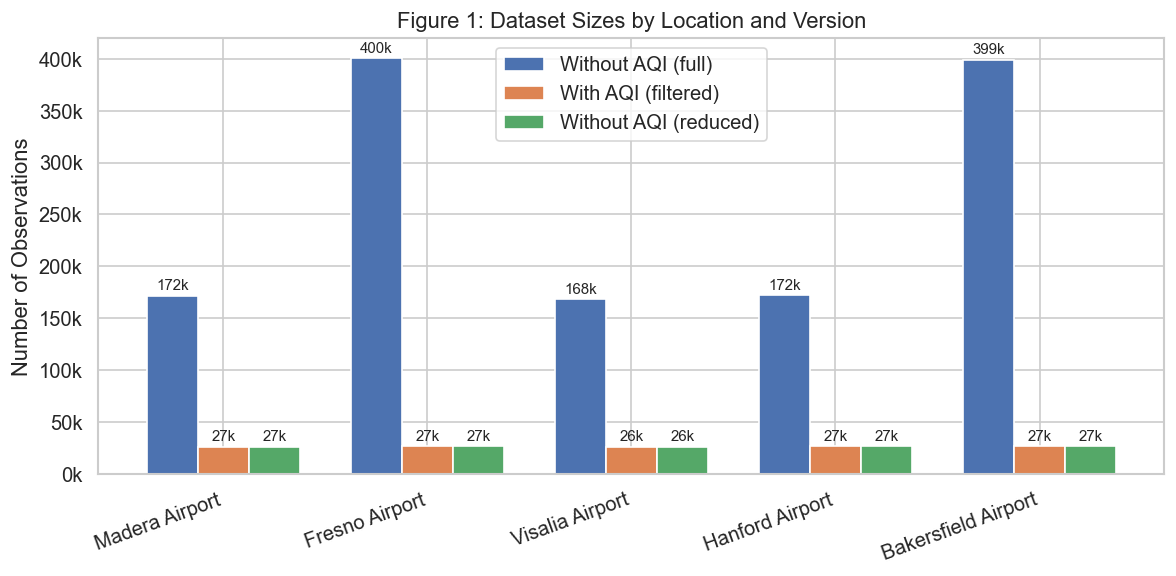
\includegraphics[keepaspectratio]{report_files/figure-pdf/cell-3-output-1.png}}

\subsection{Fog Frequency Over Time}\label{fog-frequency-over-time}

Central California's San Joaquin Valley has historically been one of the
foggiest regions in the United States, but observational evidence
suggests a long-term decline in fog occurrence. The following charts
show the annual percentage of hours classified as fog (visibility
\textless{} 1,610 m) for each monitoring location based on the
accumulated METAR-based datasets.

\pandocbounded{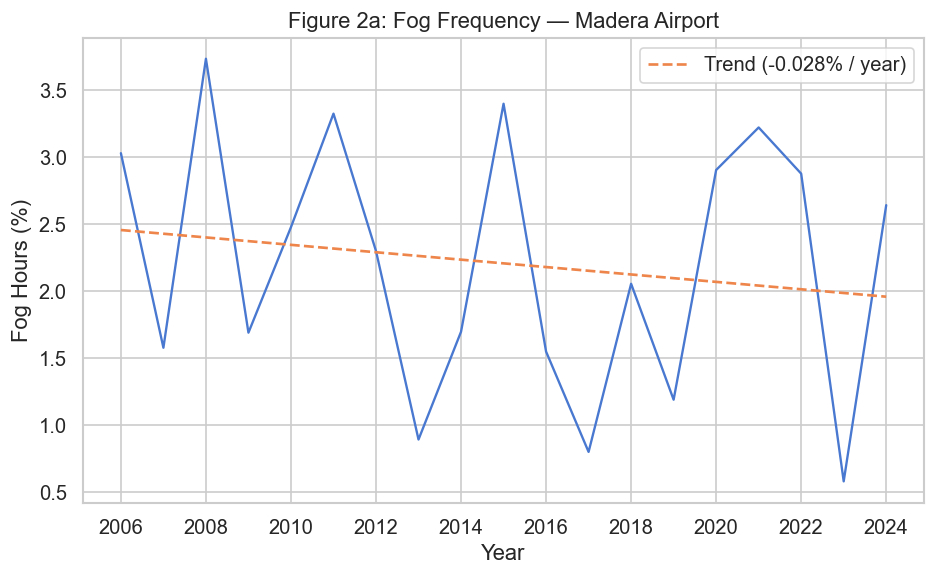
\includegraphics[keepaspectratio]{report_files/figure-pdf/cell-4-output-1.png}}

\pandocbounded{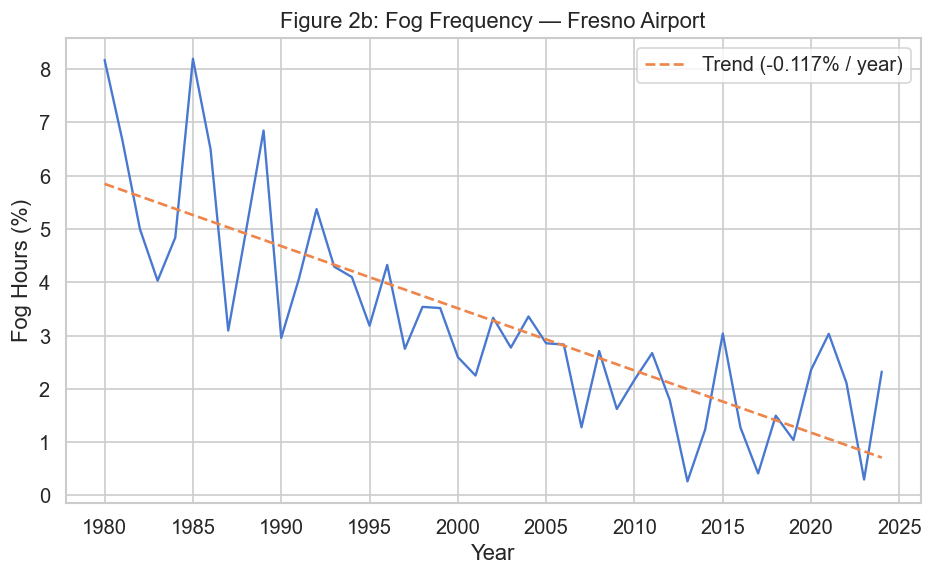
\includegraphics[keepaspectratio]{report_files/figure-pdf/cell-4-output-2.png}}

\pandocbounded{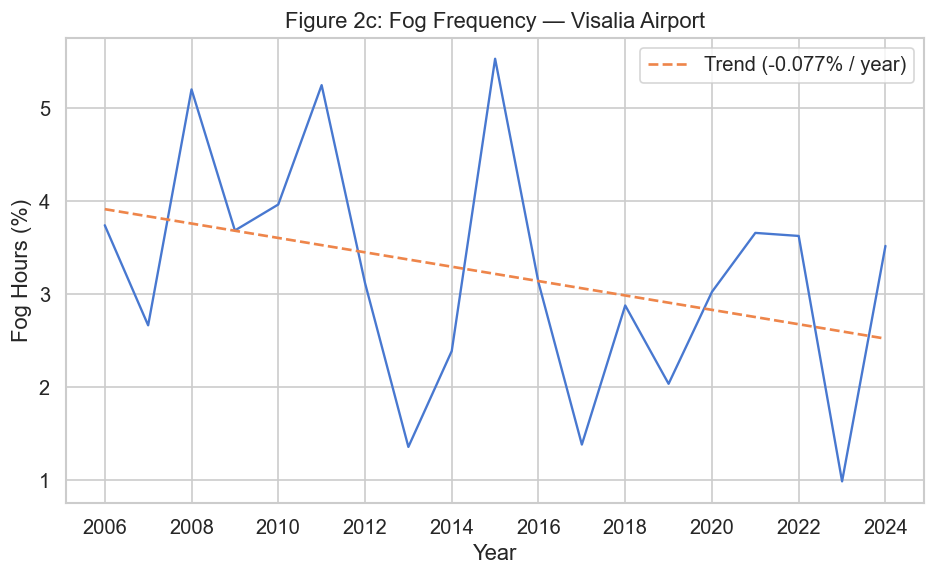
\includegraphics[keepaspectratio]{report_files/figure-pdf/cell-4-output-4.png}}

\pandocbounded{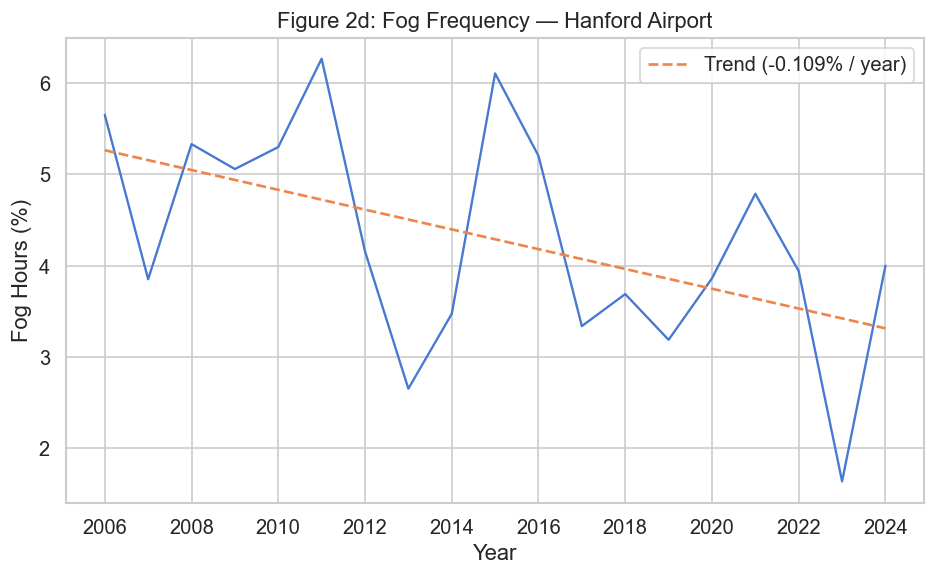
\includegraphics[keepaspectratio]{report_files/figure-pdf/cell-4-output-5.png}}

\pandocbounded{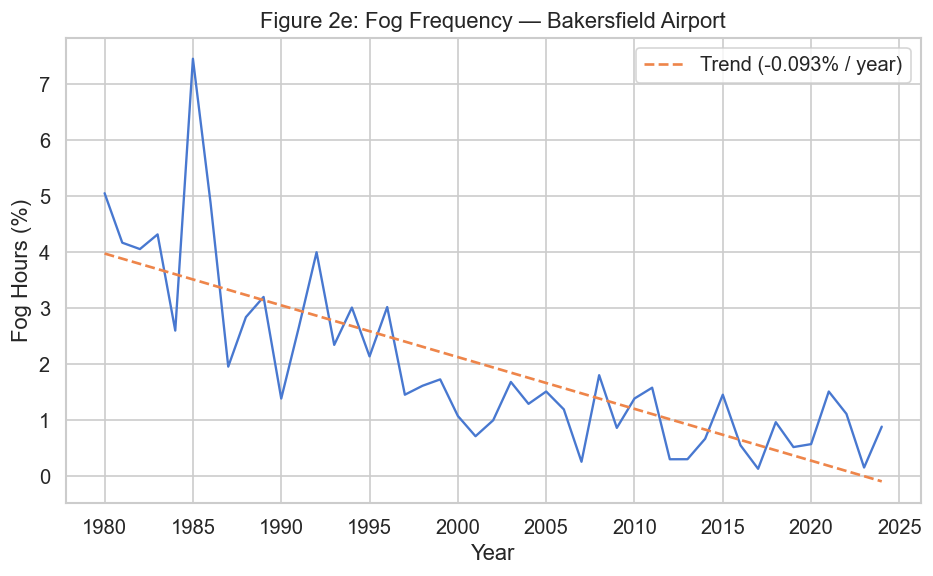
\includegraphics[keepaspectratio]{report_files/figure-pdf/cell-4-output-7.png}}

The declining fog frequency trends observed across all locations present
a significant challenge for model development and analysis, particularly
when working with the limited AQI datasets. As fog events become less
frequent over time, the number of positive fog cases available for
training and testing decreases proportionally, resulting in increasingly
imbalanced datasets. This class imbalance reduces the observable signal
strength and makes it more difficult for models to learn the
distinguishing characteristics of fog formation conditions.

The impact is especially pronounced for the AQI datasets, which are
already constrained by:

\begin{enumerate}
\def\labelenumi{\arabic{enumi}.}
\tightlist
\item
  \textbf{Temporal limitations}: AQI measurements are only available
  from 2022 onwards, providing a much shorter observation window
  compared to the weather-based datasets that span decades
\item
  \textbf{Reduced fog instances}: With fog frequency declining, the 2-3
  year AQI observation period captures fewer fog events than earlier
  periods would have
\item
  \textbf{Statistical power}: The combination of limited temporal
  coverage and declining fog frequency means there may be insufficient
  positive cases to robustly identify relationships between air quality
  variables and fog formation
\end{enumerate}

This declining signal is particularly problematic for evaluating the
predictive value of AQI variables. While these air quality measurements
may theoretically influence fog formation through their effects on
condensation nuclei availability, the limited number of fog events in
the AQI observation window makes it challenging to distinguish genuine
causal relationships from noise in the data. Consequently, any
conclusions about the importance of AQI variables for fog prediction
must be interpreted cautiously, recognizing that the observable signal
strength may be insufficient to detect moderate effects even if they
exist.

\subsection{AQI Over Time}\label{aqi-over-time}

Understanding the temporal patterns of air quality variables is
essential for contextualizing their potential role in fog formation.
Below monthly mean concentrations of four key air quality indicators are
presented: particulate matter (PM10 and PM2.5), dust, and nitrogen
dioxide. Each of these pollutants can influence atmospheric visibility
and potentially fog formation through distinct physical mechanisms.

\pandocbounded{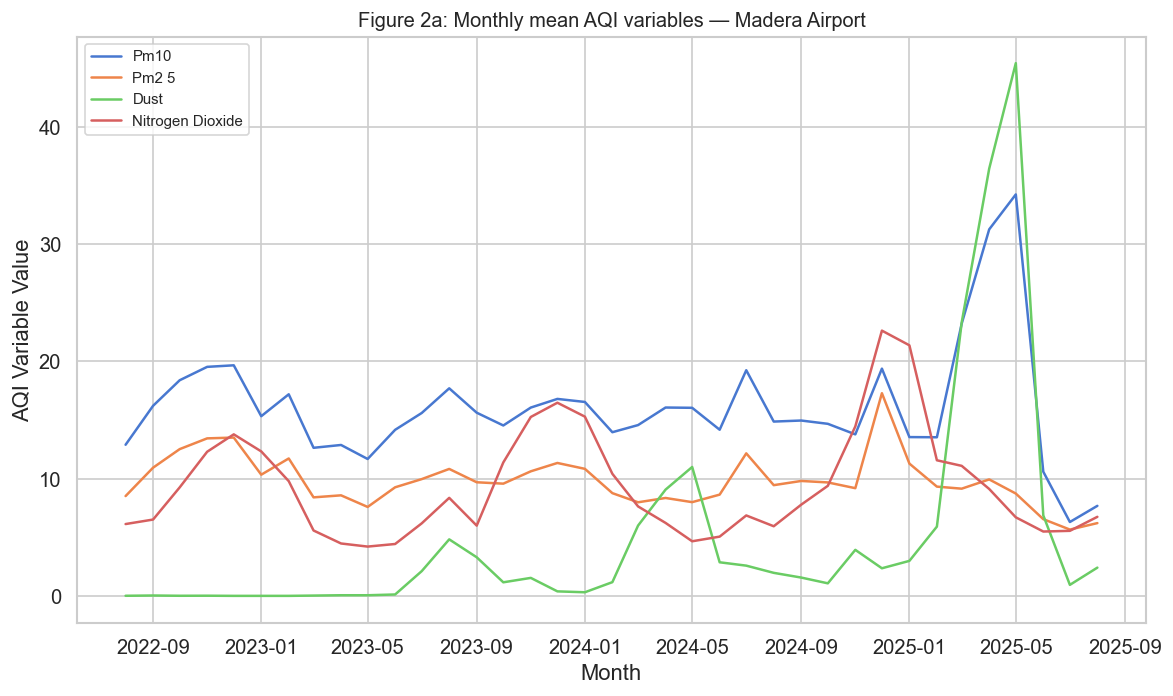
\includegraphics[keepaspectratio]{report_files/figure-pdf/cell-5-output-1.png}}

\pandocbounded{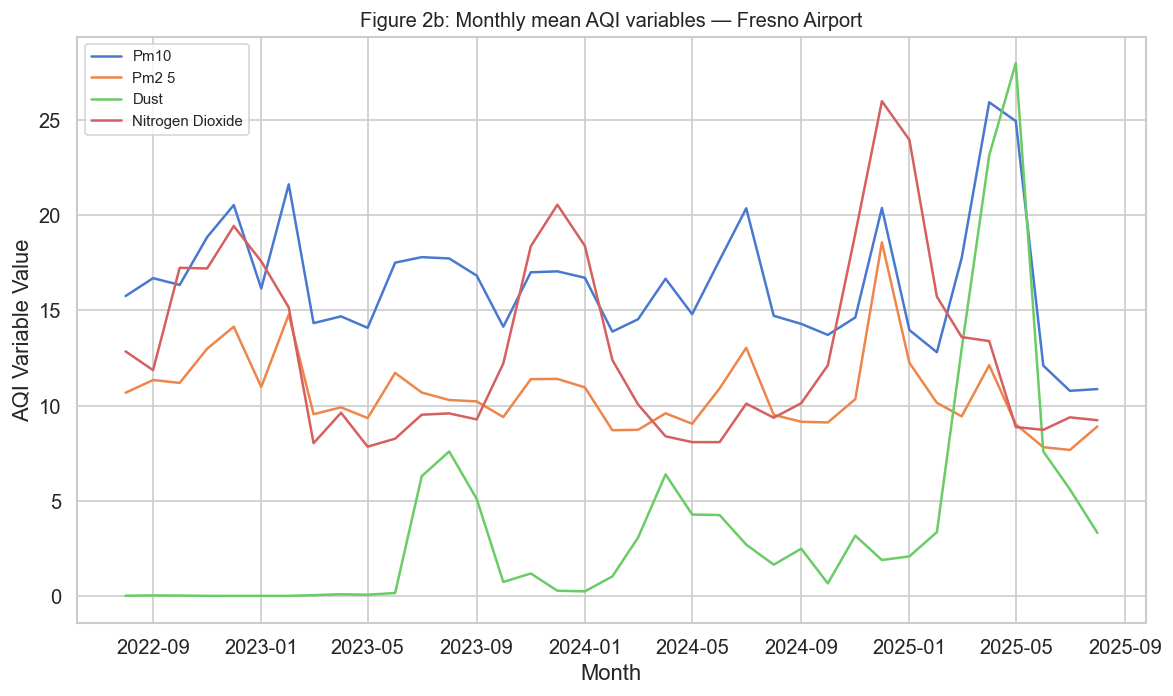
\includegraphics[keepaspectratio]{report_files/figure-pdf/cell-5-output-2.png}}

\pandocbounded{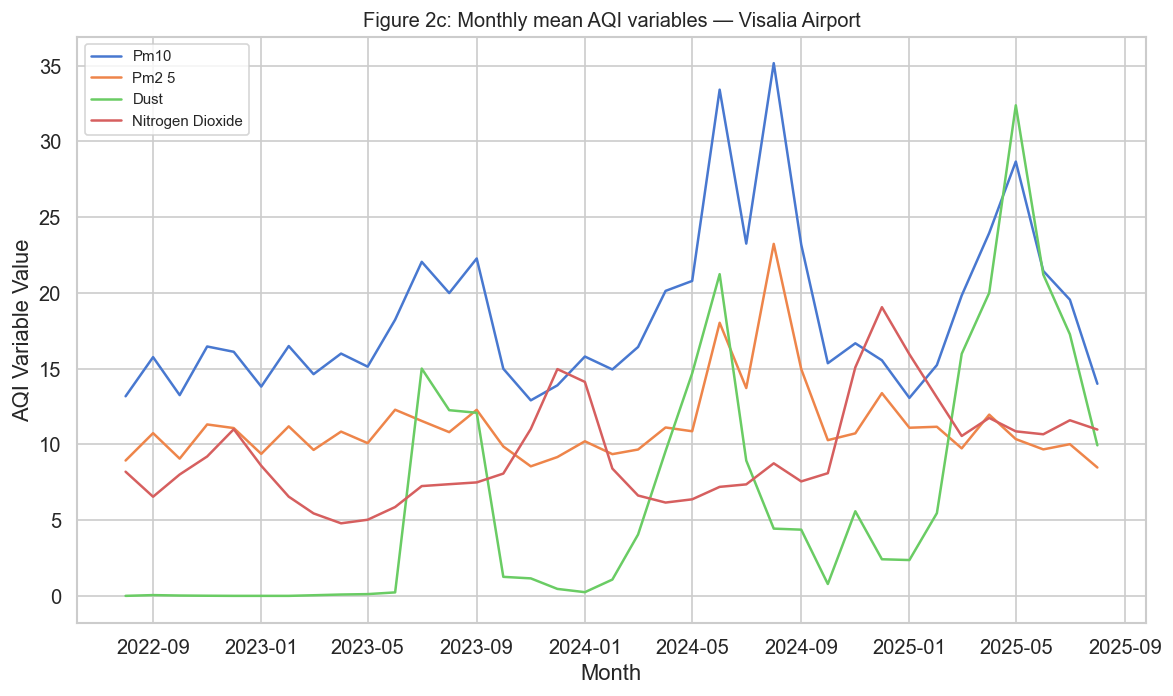
\includegraphics[keepaspectratio]{report_files/figure-pdf/cell-5-output-4.png}}

\pandocbounded{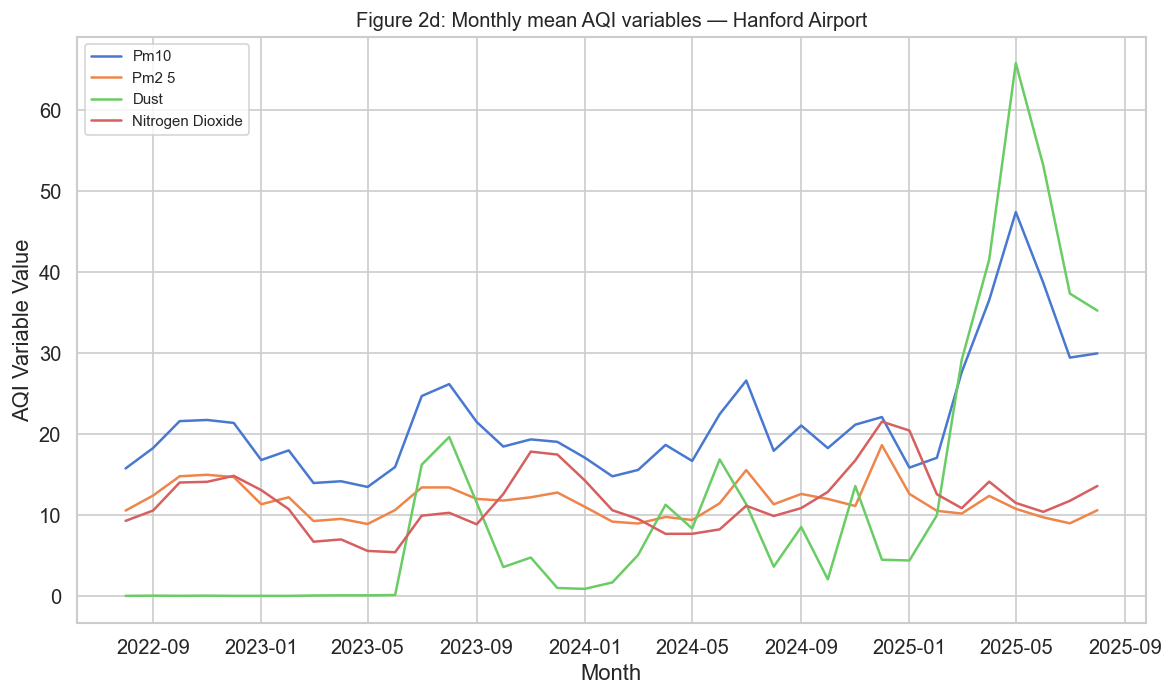
\includegraphics[keepaspectratio]{report_files/figure-pdf/cell-5-output-5.png}}

\pandocbounded{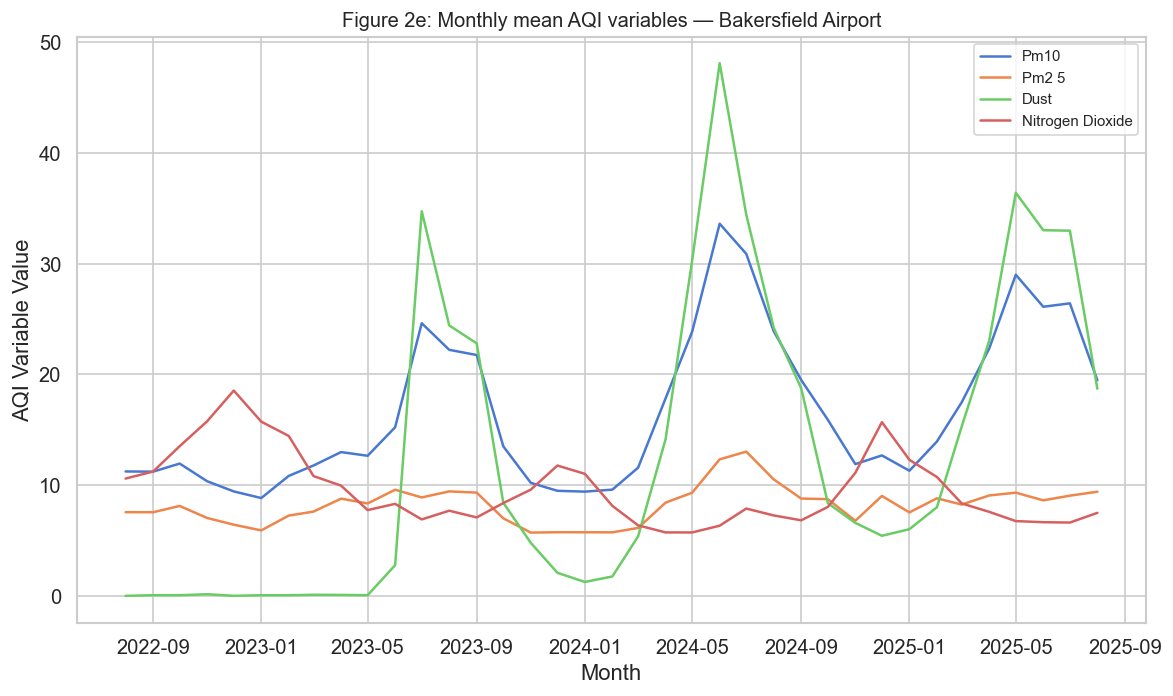
\includegraphics[keepaspectratio]{report_files/figure-pdf/cell-5-output-7.png}}

\pandocbounded{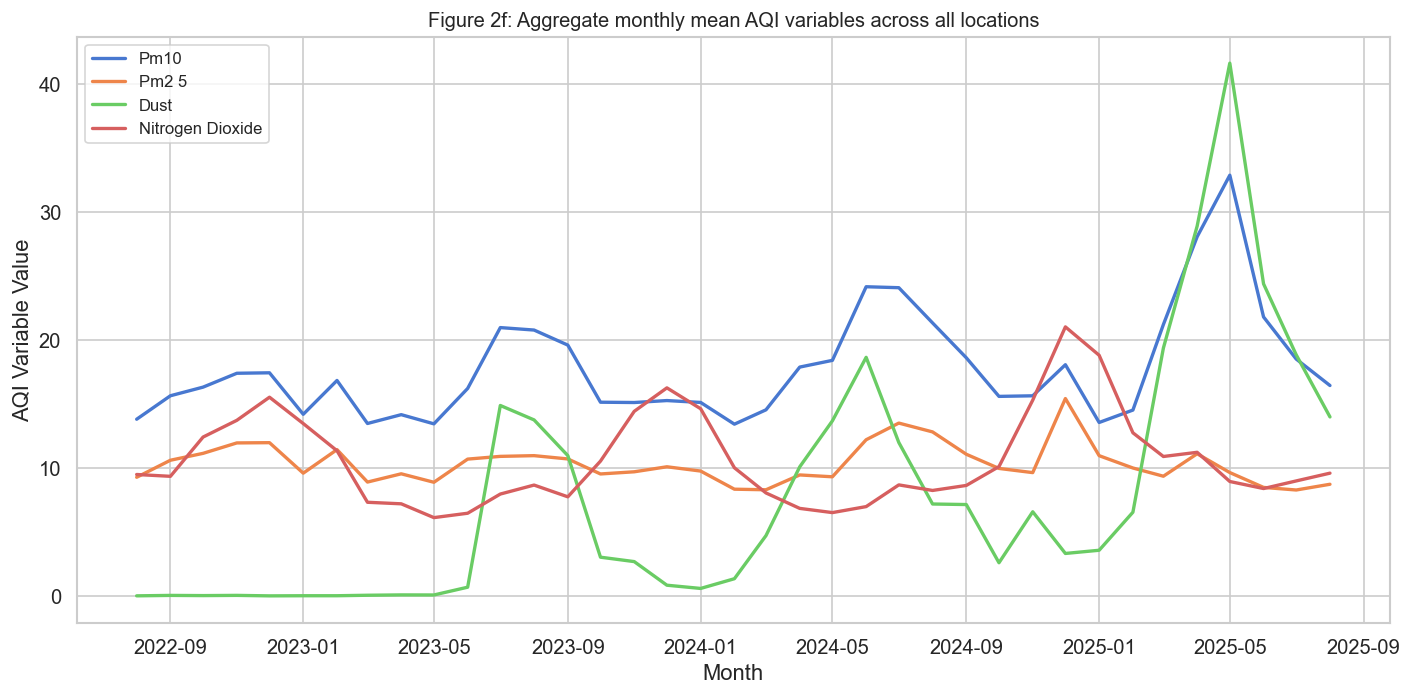
\includegraphics[keepaspectratio]{report_files/figure-pdf/cell-5-output-8.png}}

Examination of the monthly mean time series for PM10, PM2.5, dust, and
nitrogen dioxide across the five airport locations reveals no strong
systematic temporal trends over the 2022-present observation period.
While the plots exhibit month-to-month variability consistent with
meteorological influences, emission patterns, and measurement
uncertainty, there are no obvious monotonic increases or decreases that
would suggest fundamental shifts in air quality conditions during this
timeframe. The absence of pronounced trends indicates that any
year-to-year changes in air quality are relatively modest compared to
the seasonal and short-term fluctuations inherent in these measurements.

This lack of strong temporal trends is methodologically advantageous for
this fog prediction analysis. Had there been significant upward or
downward drifts in pollutant concentrations coinciding with the
declining fog frequency, this would have possibly introduced noise into
the dataset, thereby undercutting model efficiency. This risk is
especially exacerbated by the low amount of availably AQI data. In
latter portions of this analysis, the limitations of the test/train
split are discussed. Specifically, the limitation of the AQI-reliant
dataset size results in only two full, complete years being available
for analysis. Had there been a significant monotonic drifts in AQI
variability, this would have possibly polluted one or both of the
test/train datasets.

\subsection{Predictor Correlations with
Visibility}\label{predictor-correlations-with-visibility}

To assess the linear relationships between predictor variables and
visibility, Pearson correlation coefficients were computed for each
variable group: \textbf{weather}, \textbf{AQI}, and \textbf{inferred}.
The bar charts below present the average absolute correlation strength
by variable category across all five airport locations; these values are
sorted in descending order. These aggregated visualizations provide a
high-level comparison of which variable groups exhibit the strongest
relationships with visibility. Complete per-location Pearson correlation
tables, showing individual correlation coefficients for each predictor
at each airport, are available in \textbf{Appendix A}.

\pandocbounded{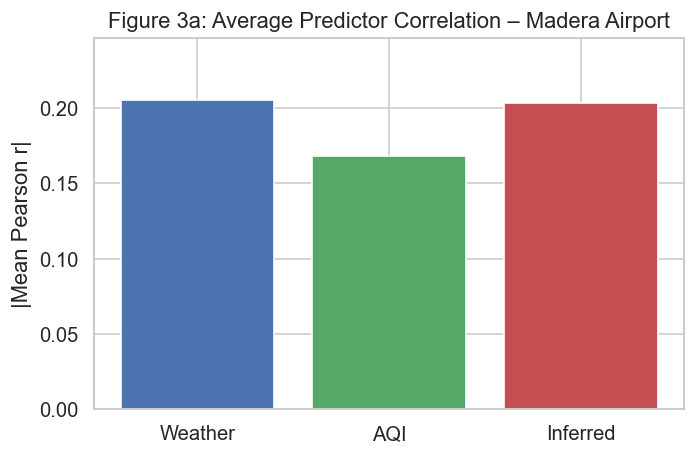
\includegraphics[keepaspectratio]{report_files/figure-pdf/cell-7-output-1.png}}

\pandocbounded{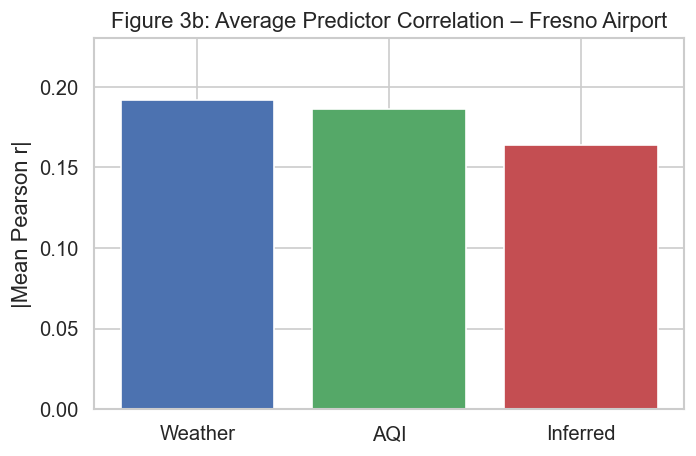
\includegraphics[keepaspectratio]{report_files/figure-pdf/cell-7-output-2.png}}

\pandocbounded{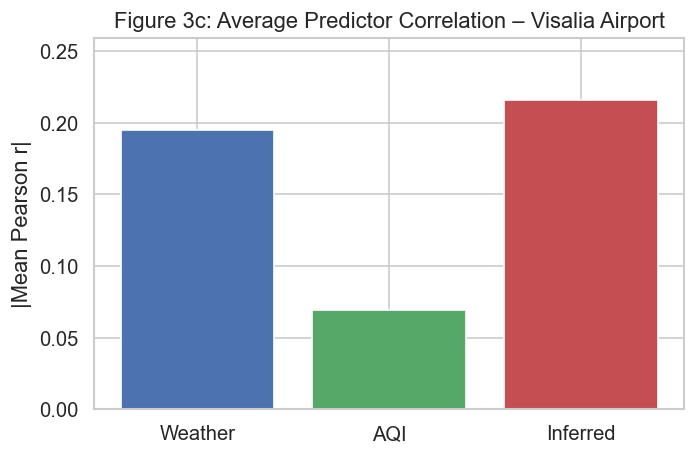
\includegraphics[keepaspectratio]{report_files/figure-pdf/cell-7-output-4.png}}

\pandocbounded{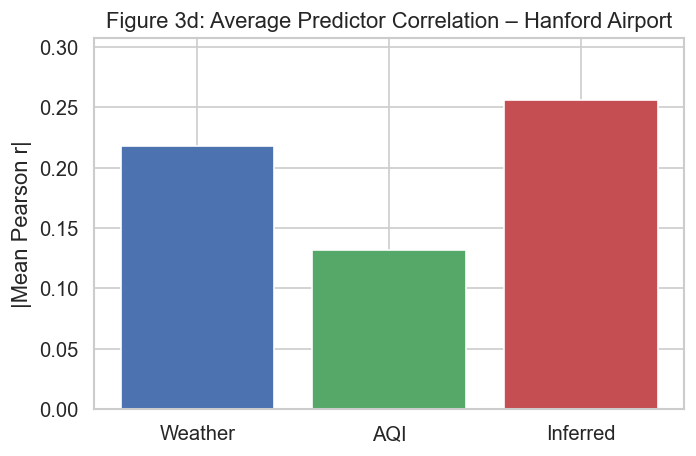
\includegraphics[keepaspectratio]{report_files/figure-pdf/cell-7-output-5.png}}

\pandocbounded{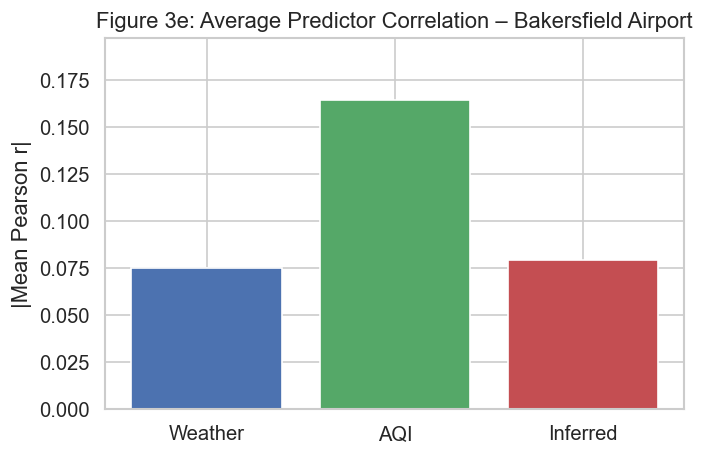
\includegraphics[keepaspectratio]{report_files/figure-pdf/cell-7-output-7.png}}

\pandocbounded{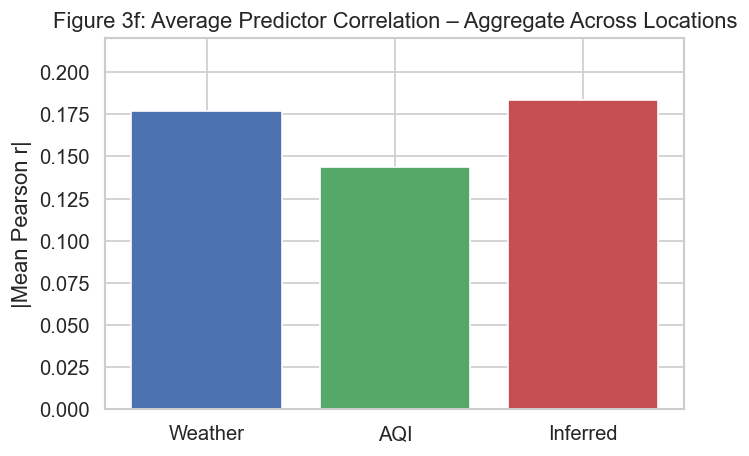
\includegraphics[keepaspectratio]{report_files/figure-pdf/cell-7-output-8.png}}

The aggregate correlation analysis reveals that raw weather and inferred
variables exhibit the strongest average linear relationship with
visibility, followed by AQI variables showing the weakest but still
meaningful correlations. Despite AQI variables having lower average
absolute Pearson correlation coefficients compared to the weather and
inferred predictors, their correlations remain statistically relevant
and justify their inclusion as candidate features in fog prediction
models. The reduced correlation strength is expected given the limited
temporal coverage of AQI data compared to the multi-decadal weather
records, which constrains the sample size available for estimating these
relationships.

Importantly, the correlation strength of AQI variables exhibits
substantial spatial heterogeneity across the five airport locations. The
enhanced AQI signal at Bakersfield may reflect local emission patterns,
topographic influences on pollutant accumulation, or site-specific
meteorological regimes that amplify the relationship between air quality
and visibility conditions. These location-dependent differences
underscore the value of training separate models for each airport rather
than pooling data across sites.

\section{Feature Distributions: Fog
vs.~Non-Fog}\label{feature-distributions-fog-vs.-non-fog}

\subsection{Examination of Weather
Variables}\label{examination-of-weather-variables}

To understand how individual predictors differ between fog and non-fog
conditions, their distributions were compared using box plots. Features
are z-score standardized to allow comparison on a common axis. Separate
plots are shown for \textbf{weather variables}, \textbf{AQI variables},
and \textbf{inferred variables} at each airport and in aggregate.

\pandocbounded{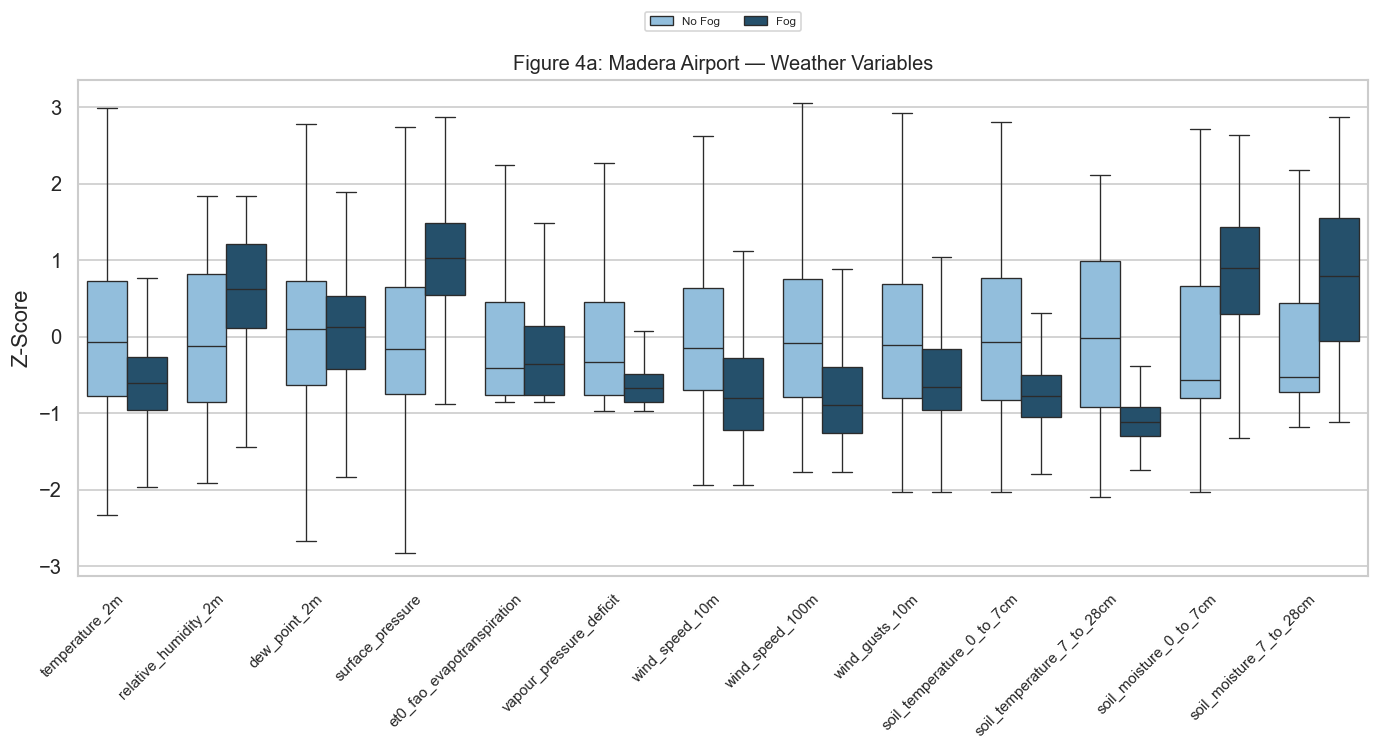
\includegraphics[keepaspectratio]{report_files/figure-pdf/cell-8-output-1.png}}

\pandocbounded{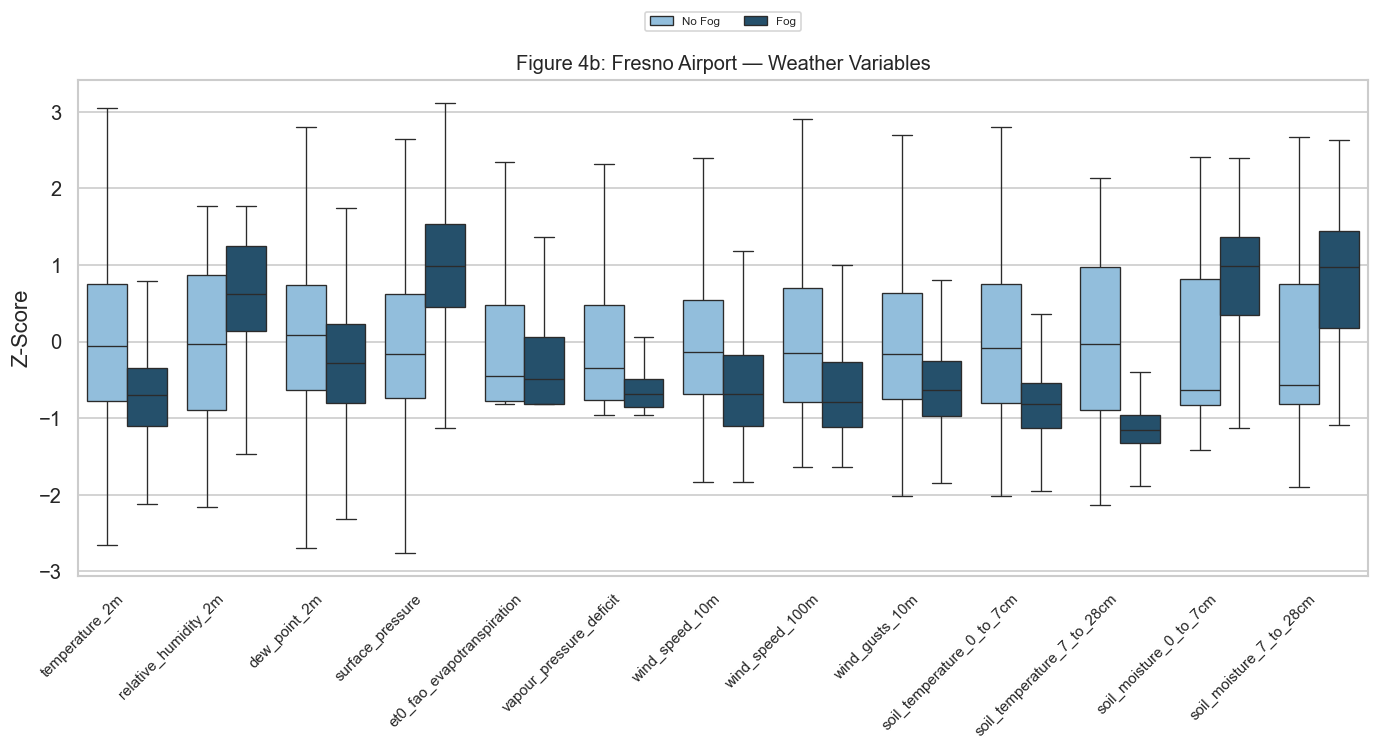
\includegraphics[keepaspectratio]{report_files/figure-pdf/cell-8-output-2.png}}

\pandocbounded{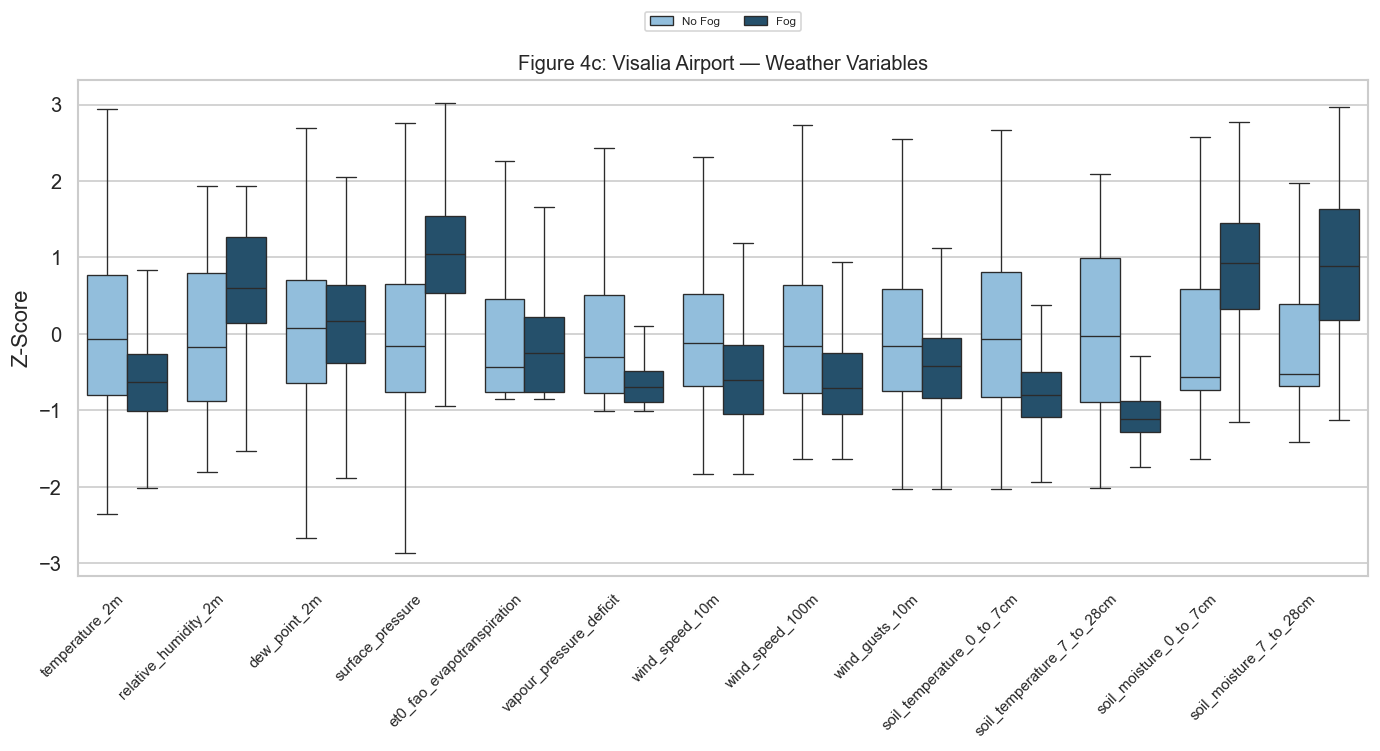
\includegraphics[keepaspectratio]{report_files/figure-pdf/cell-8-output-3.png}}

\pandocbounded{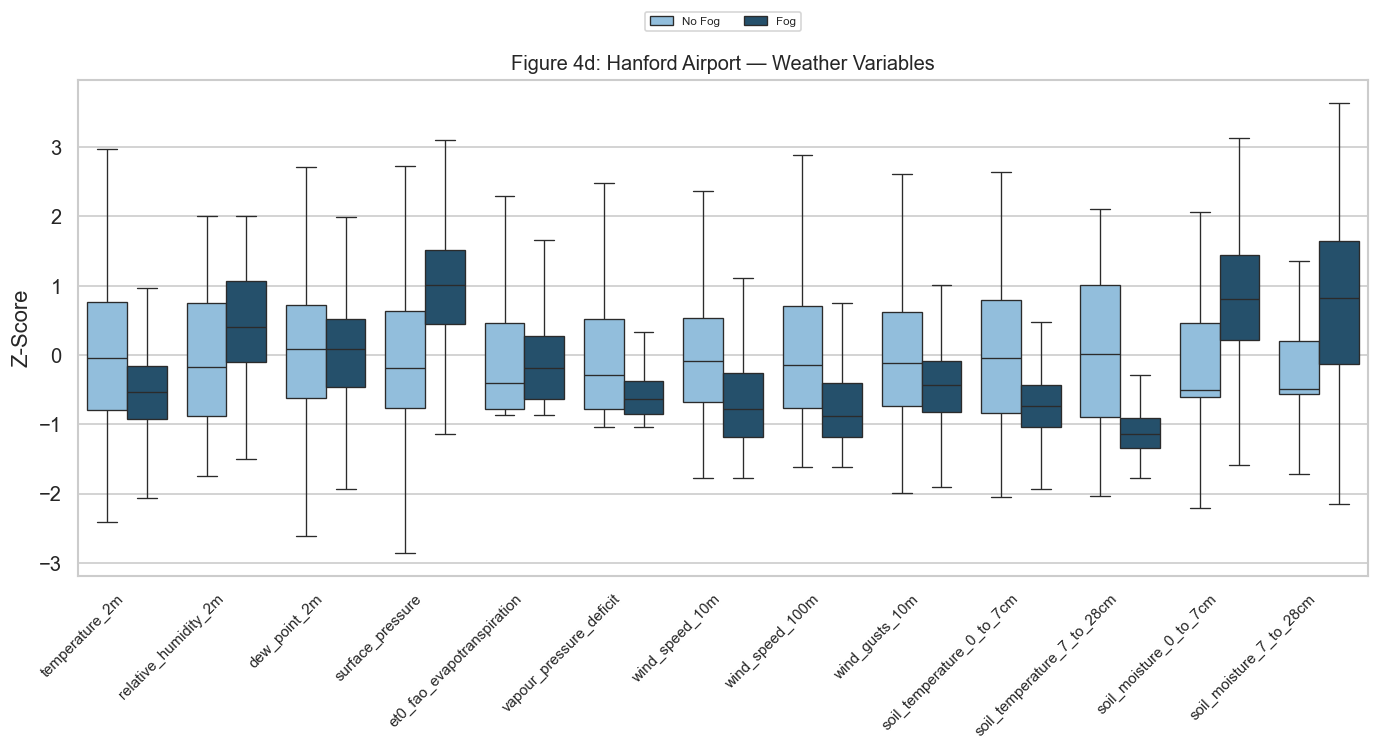
\includegraphics[keepaspectratio]{report_files/figure-pdf/cell-8-output-5.png}}

\pandocbounded{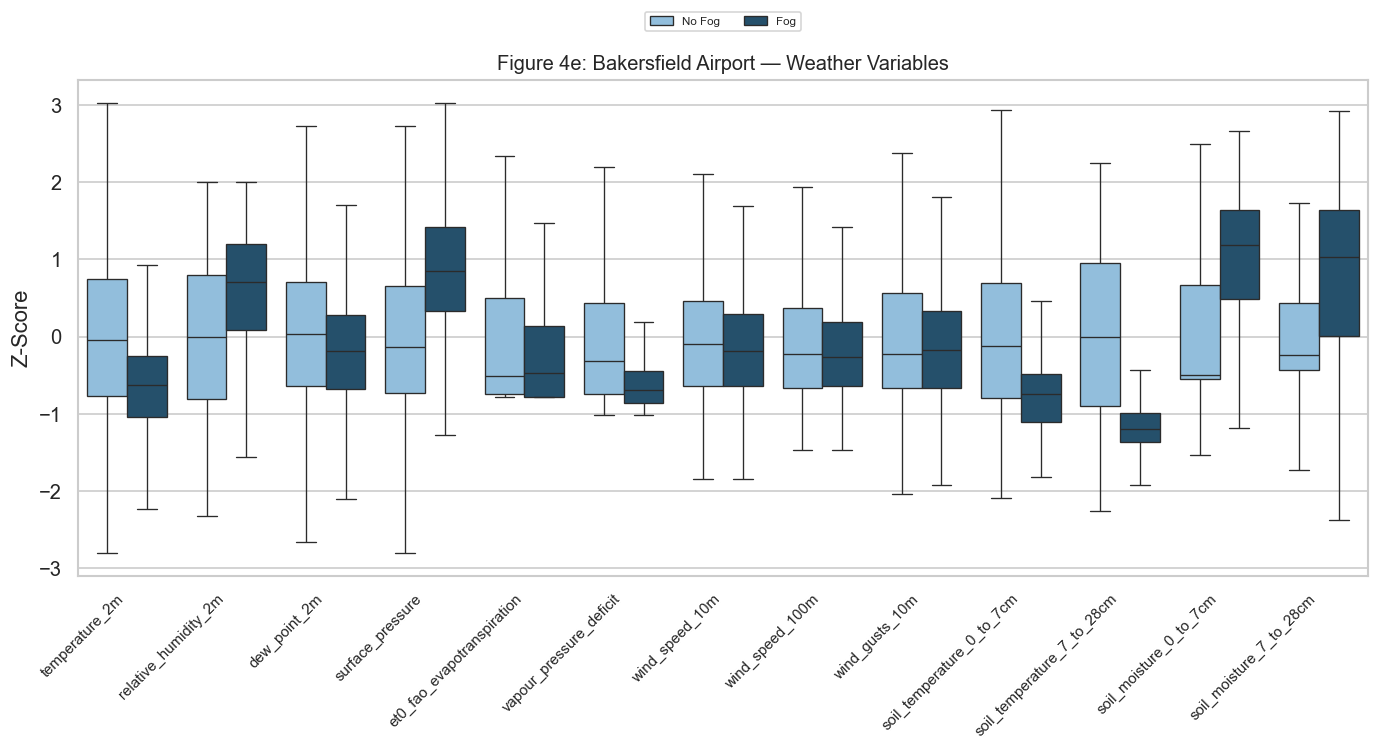
\includegraphics[keepaspectratio]{report_files/figure-pdf/cell-8-output-6.png}}

\pandocbounded{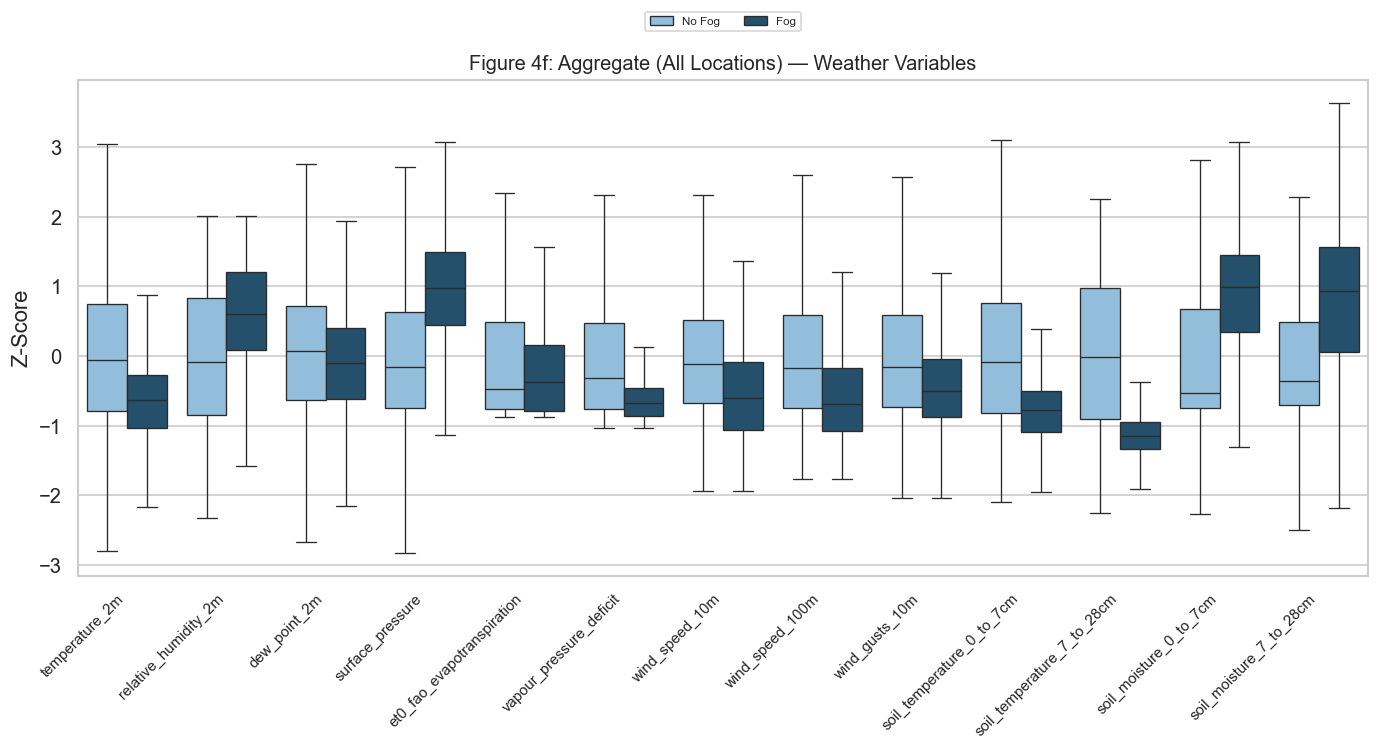
\includegraphics[keepaspectratio]{report_files/figure-pdf/cell-8-output-7.png}}

The box plot distributions reveal systematic differences in predictor
values between fog and non-fog conditions that align with the
fundamental physics of radiation fog formation. Fog events exhibit
significantly higher standardized values for relative humidity, surface
pressure, evapotranspiration, and soil moisture at both the 0-7 cm and
7-28 cm depths. Conversely, fog conditions are associated with lower
values for temperature, dew point depression, wind speeds, wind gusts,
soil temperature at both measurement depths, and vapor pressure deficit.
These distributional patterns are strongly consistent with the
established meteorological conditions that promote radiation fog
development. Overall, there appears a distinct, measurable signal within
all variables that should promote binary classification via machine
learning.

\subsection{Examination of Rain \&
Precipitation}\label{examination-of-rain-precipitation}

The precipitation and rain variables were intentionally excluded from
the weather variable box plots presented above due to their extremely
low incidence rates across all locations. As shown in the table below,
these variables have zero values for the vast majority of observations
(\textgreater95\% across all locations). This reflects the semi-arid
climate of the San Joaquin Valley where precipitation events are rare.
When included in the standardized box plots alongside other weather
variables, the high frequency of zero values causes the interquartile
ranges to collapse near zero, producing compressed box plots that are
visually uninformative and difficult to interpret relative to the other
predictors.

To meaningfully examine the distributions of precipitation and rain
during fog versus non-fog conditions, a conditional analysis was applied
that filters the dataset to include only observations where
precipitation or rain values are strictly greater than zero. This subset
provides a more interpretable comparison of how these variables behave
when precipitation is actually occurring. The filtered box plots below
present the fog versus non-fog distributions for this
precipitation-active subset of the data.

\begin{longtable}[]{@{}llll@{}}
\toprule\noalign{}
& Location & Precipitation = 0 (\%) & Rain = 0 (\%) \\
\midrule\noalign{}
\endhead
\bottomrule\noalign{}
\endlastfoot
0 & Madera Airport & 0.95 & 0.95 \\
1 & Fresno Airport & 0.94 & 0.94 \\
2 & Visalia Airport & 0.95 & 0.95 \\
3 & Hanford Airport & 0.96 & 0.96 \\
4 & Bakersfield Airport & 0.94 & 0.94 \\
\end{longtable}

\pandocbounded{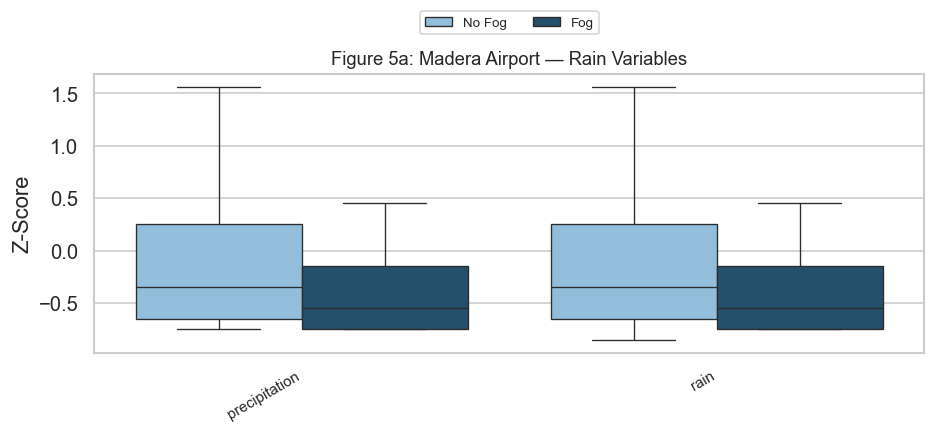
\includegraphics[keepaspectratio]{report_files/figure-pdf/cell-10-output-1.png}}

\pandocbounded{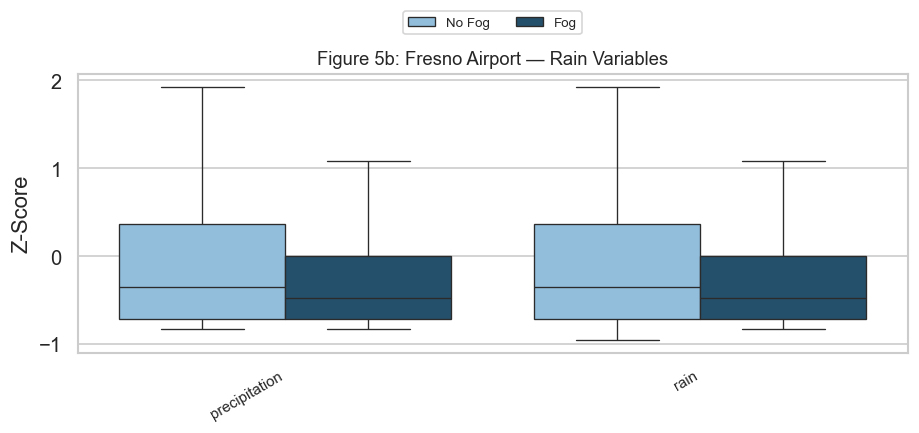
\includegraphics[keepaspectratio]{report_files/figure-pdf/cell-10-output-2.png}}

\pandocbounded{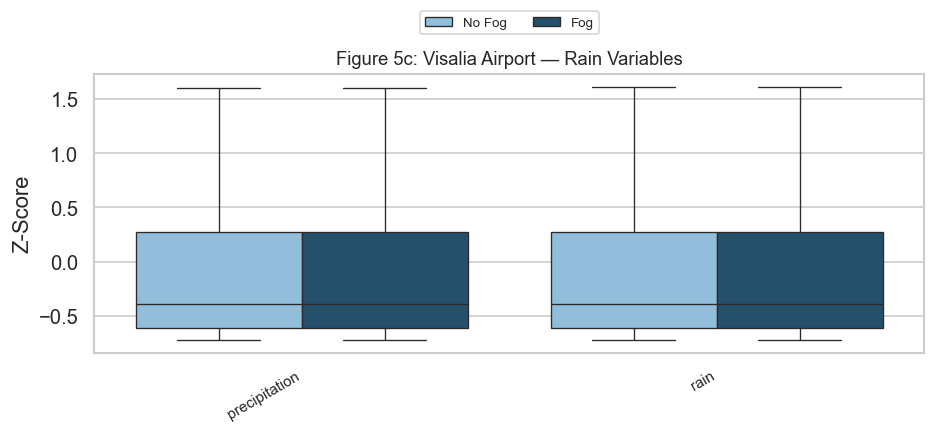
\includegraphics[keepaspectratio]{report_files/figure-pdf/cell-10-output-3.png}}

\pandocbounded{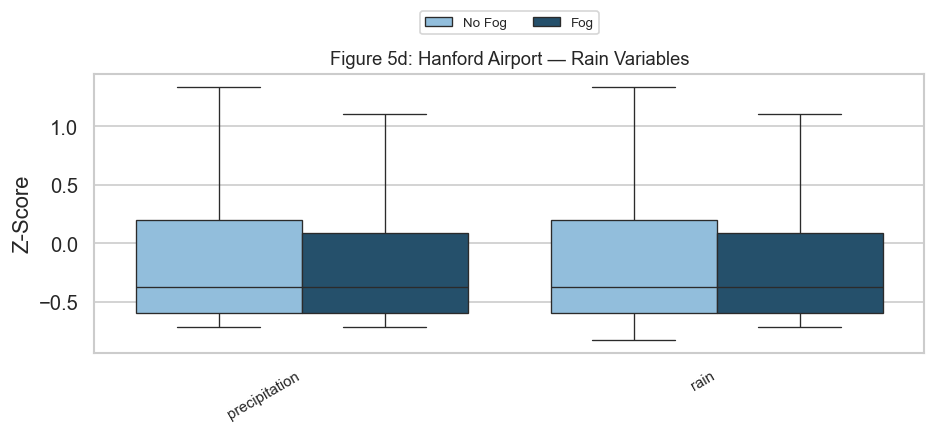
\includegraphics[keepaspectratio]{report_files/figure-pdf/cell-10-output-5.png}}

\pandocbounded{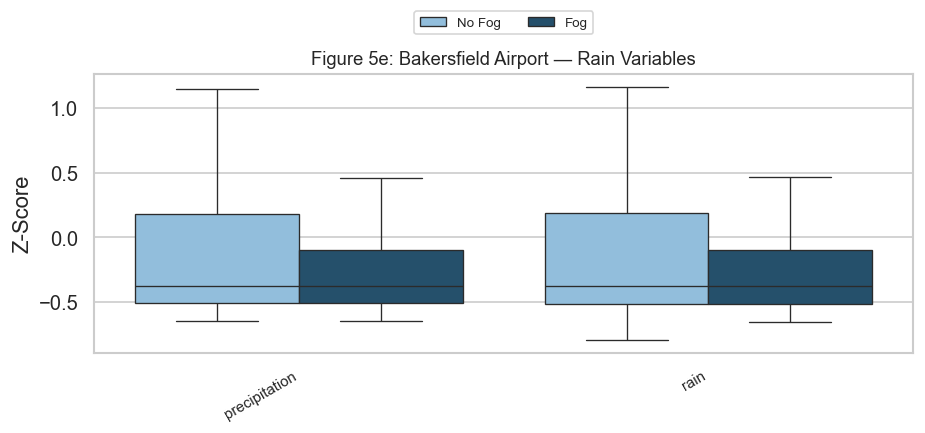
\includegraphics[keepaspectratio]{report_files/figure-pdf/cell-10-output-6.png}}

\pandocbounded{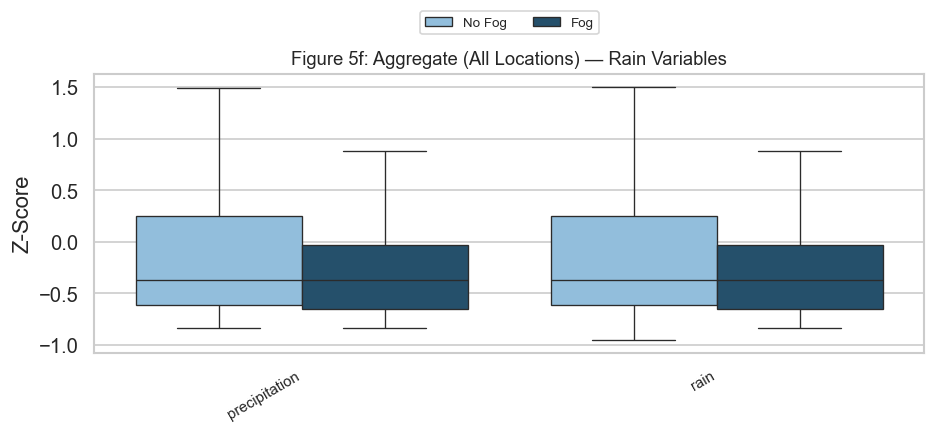
\includegraphics[keepaspectratio]{report_files/figure-pdf/cell-10-output-7.png}}

When examining only observations with non-zero precipitation or rain,
the box plot distributions show subtle albeit meaningful differences
between fog and non-fog conditions despite having similar mean values.
The central tendencies of precipitation during fog versus non-fog events
appear comparable, suggesting that precipitation intensity alone may not
strongly differentiate these conditions. However, the box plots
consistently show differences in the interquartile ranges, whisker
extents, and overall distributional shapes between the two classes
across locations.

These distributional differences are particularly relevant because
precipitation and rain variables exhibit strongly left-skewed
distributions when filtered to non-zero values. This skewness implies
that summary statistics like the mean can be misleading, as they do not
fully capture the shape of the distribution. however, the box plots,
when considered within their contexts, reveal that fog and non-fog
conditions differ not just in average precipitation amount, but in the
spread and quantile structure of the distributions. These shape
differences may reflect distinct meteorological processes: fog
associated with lighter, more persistent drizzle versus non-fog
conditions experiencing heavier, convective-type precipitation.
Consequently, even modest distributional shifts visible in the box plots
represent physically meaningful differences in precipitation
characteristics that could inform model predictions, despite the
similarity in mean values.

An important caveat in the above analysis is the possibility of causal
ambiguity in the relationship between precipitation and observed fog
events. In the above analysis, the conditions are categorized as ``fog''
when the reduced visibility is less than the 1-mile (1610 m) threshold,
without regard to the underlying meteorological process. The larger
context in which this analysis is performed deals with the phenomenon of
radiation fog, while precipitation can result in reduced visibility
through several mechanisms. This implies the possibility that the
conditions categorized as ``fog'' in the data could be the result of
reduced visibility caused by precipitation, as opposed to the
traditional phenomenon of radiation fog. This, however, does not detract
from the categorization as ``fog,'' as reduced visibility is a genuine
operational hazard, irrespective of the underlying process. However,
this implies that the models using precipitation features could be
improved by including this as an additional type of fog, even though
this could be a small percentage of the total number of fog events in
the semi-arid region of the San Joaquin Valley.

\subsection{Examination of AQI
Variables}\label{examination-of-aqi-variables}

The following analysis examines the distributions of air quality
variables (PM10, PM2.5, dust, and nitrogen dioxide) during fog versus
non-fog conditions using the same z-score standardization and box plot
methodology applied to the weather variables. These box plots are based
on the subset of data where AQI measurements are available
(2022-present).

\pandocbounded{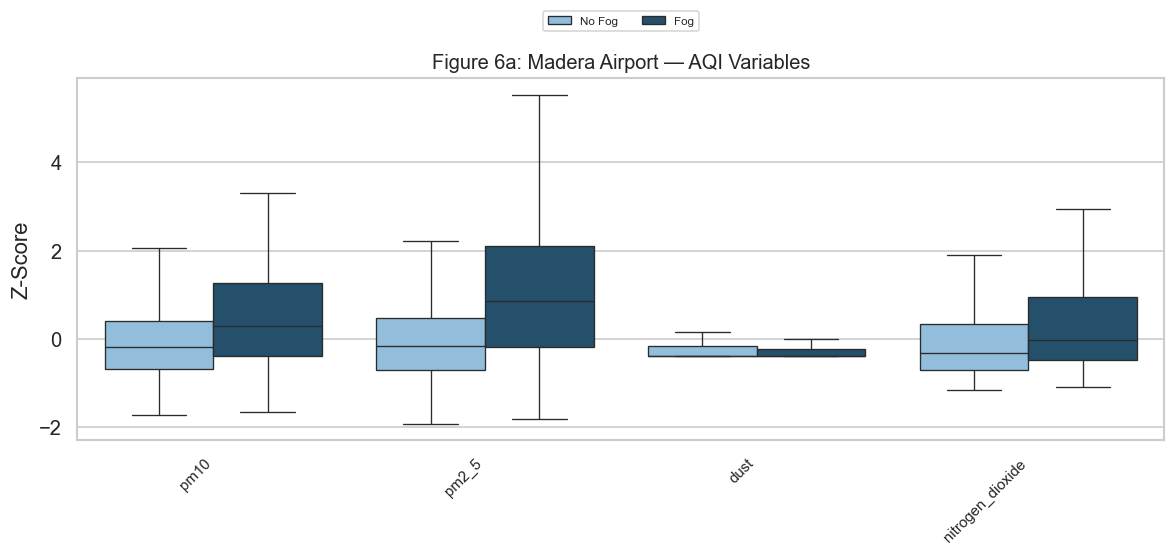
\includegraphics[keepaspectratio]{report_files/figure-pdf/cell-11-output-1.png}}

\pandocbounded{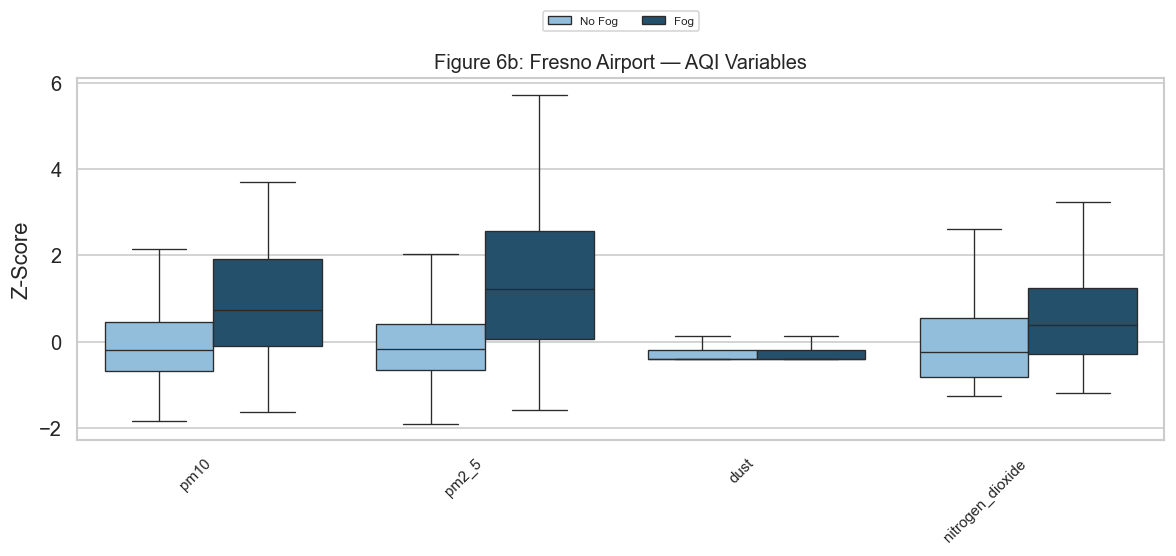
\includegraphics[keepaspectratio]{report_files/figure-pdf/cell-11-output-2.png}}

\pandocbounded{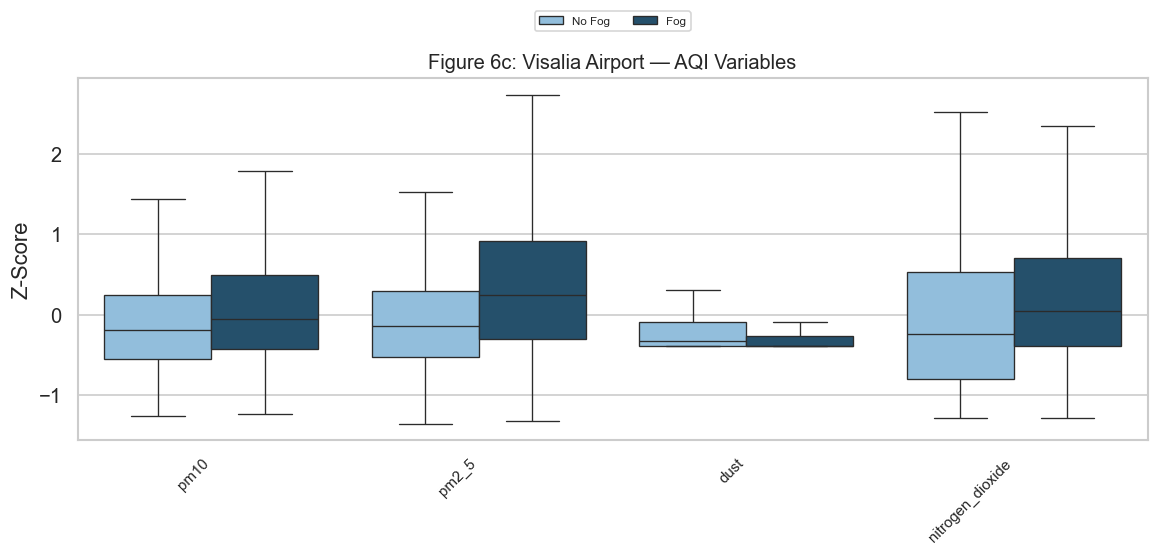
\includegraphics[keepaspectratio]{report_files/figure-pdf/cell-11-output-3.png}}

\pandocbounded{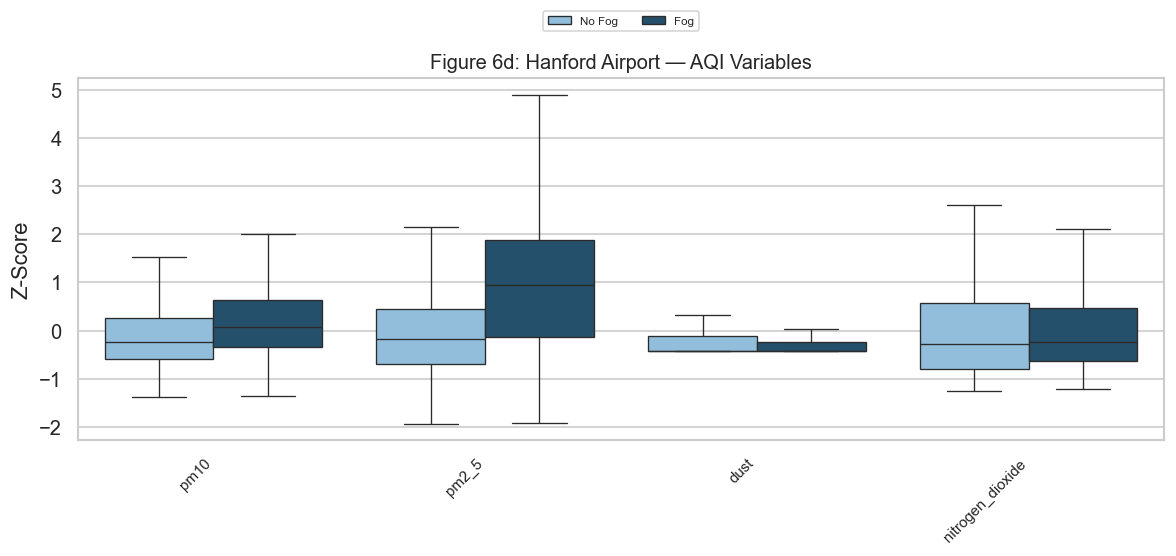
\includegraphics[keepaspectratio]{report_files/figure-pdf/cell-11-output-5.png}}

\pandocbounded{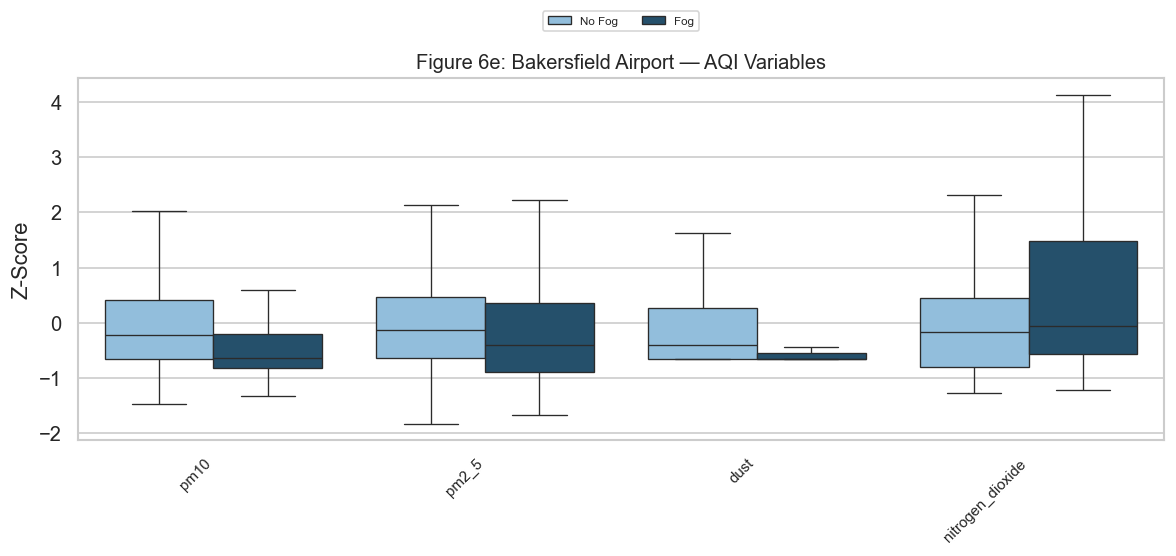
\includegraphics[keepaspectratio]{report_files/figure-pdf/cell-11-output-6.png}}

\pandocbounded{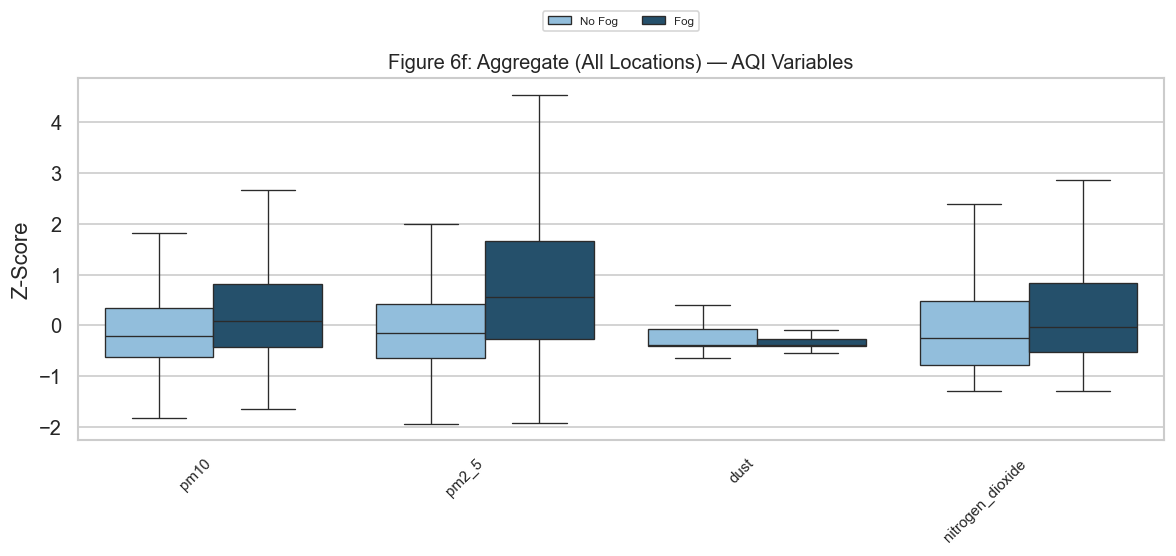
\includegraphics[keepaspectratio]{report_files/figure-pdf/cell-11-output-7.png}}

The variable box plots for the AQI data indicate clear patterns in the
distributions that differentiate fog from non-fog conditions. This
indicates that air quality data contains a useful signal for predicting
fog, even with the limited time period. Of interest is the fact that fog
is characterized by increased standardized values for PM10, PM2.5, and
nitrogen dioxide at most sites. This is consistent with the expectation
that increased concentrations of particulate matter will increase the
number of condensation nuclei available for fog formation in saturated
conditions. The consistency in the direction of difference also supports
the possibility that anthropogenic and natural aerosols may play a role
in modulating fog formation in the SJV region, especially during the
winter months when both fog formation and pollutant concentrations are
likely to be maximized due to temperature inversions.

Unlike in the case of other AQI metrics, dust concentration does not
have a clear distributional difference between the two classes. In the
box plots provided for dust concentration, it is evident that the
interquartile ranges overlap significantly and that the median values
are comparable between the two classes. However, it is important to note
that unlike in the case of other metrics such as PM2.5, PM10, and
nitrogen dioxide, the interquartile range for dust concentration is
relatively smaller in size. This may be due to the fact that dust
concentration does not vary as widely across observations as in the case
of other metrics under consideration. In this case, it is evident that
dust concentration may have a more consistent regional background level
and that dust transport events may be less dependent upon local fog
formation mechanisms. However, it is evident that PM2.5, PM10, and
nitrogen dioxide have a greater impact upon the AQI and that dust
concentration may have a lower impact upon AQI in the context of a model
designed to predict fog formation.

\subsection{Examination of Inferred
Variables}\label{examination-of-inferred-variables}

The following analysis will look at the distributions of the four
engineered inferred variables: dewpoint depression, cooling rate 6 hour,
cooling rate 12 hour, and previous night low temperature. These inferred
variables were designed to identify thermodynamic and temporal
characteristics that are particularly relevant to nocturnal radiation
fog formation. Again, a z-score normalization is used for visualization
purposes across these inferred variables that have different scale
types.

On the basis of the physical processes that lead to radiation fog, these
variables were expected to show the strongest differences in their
distributions between fog and non-fog situations. A lower dewpoint
depression, indicating saturation of air, and a more negative cooling
rate, indicating efficient radiative cooling, together with lower
previous night minimum temperatures, all point towards fog.

\pandocbounded{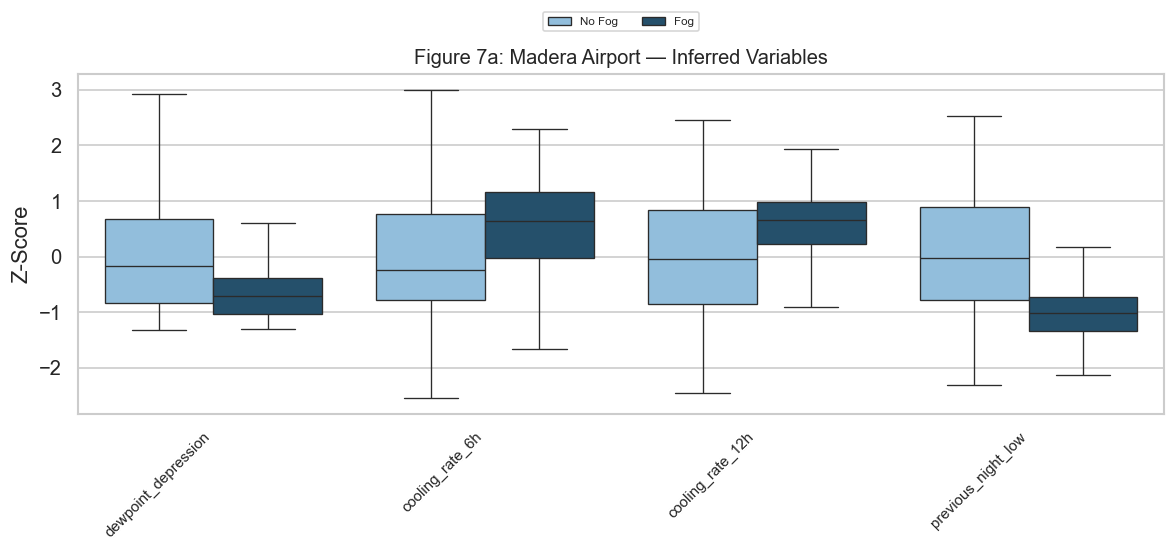
\includegraphics[keepaspectratio]{report_files/figure-pdf/cell-12-output-1.png}}

\pandocbounded{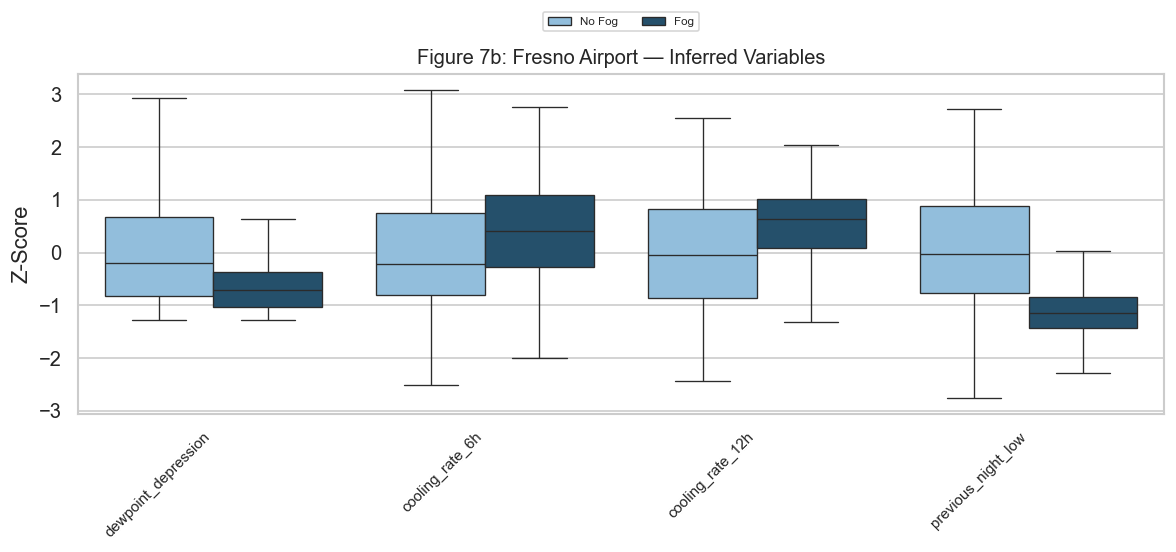
\includegraphics[keepaspectratio]{report_files/figure-pdf/cell-12-output-2.png}}

\pandocbounded{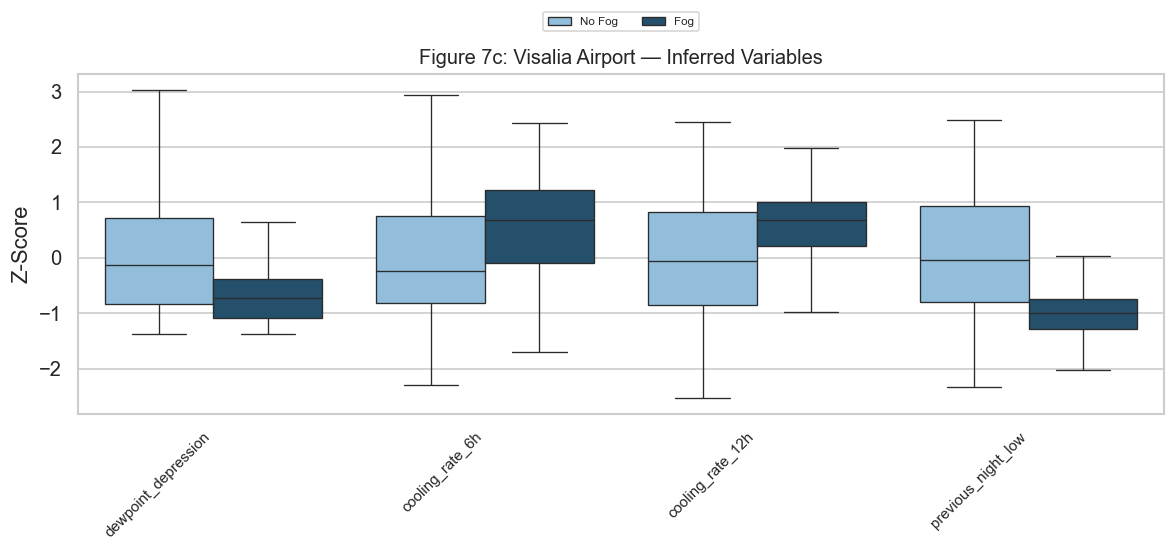
\includegraphics[keepaspectratio]{report_files/figure-pdf/cell-12-output-3.png}}

\pandocbounded{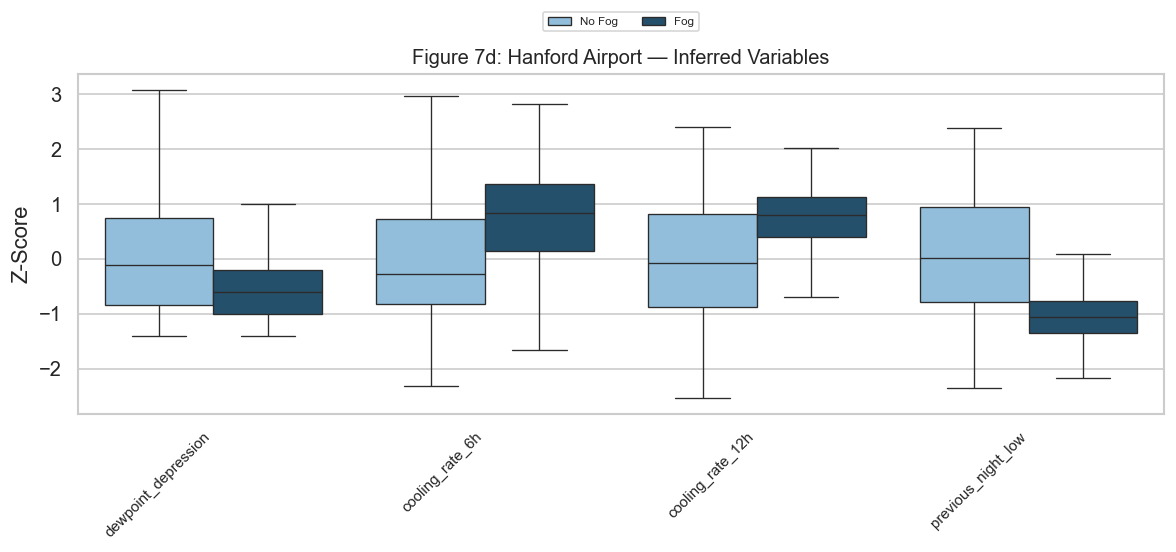
\includegraphics[keepaspectratio]{report_files/figure-pdf/cell-12-output-5.png}}

\pandocbounded{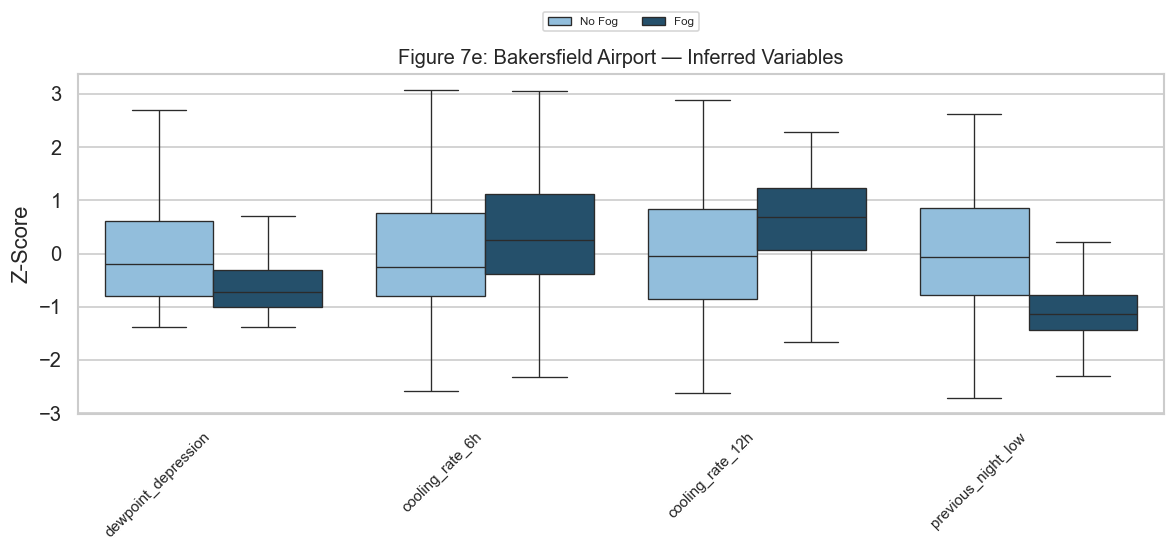
\includegraphics[keepaspectratio]{report_files/figure-pdf/cell-12-output-6.png}}

\pandocbounded{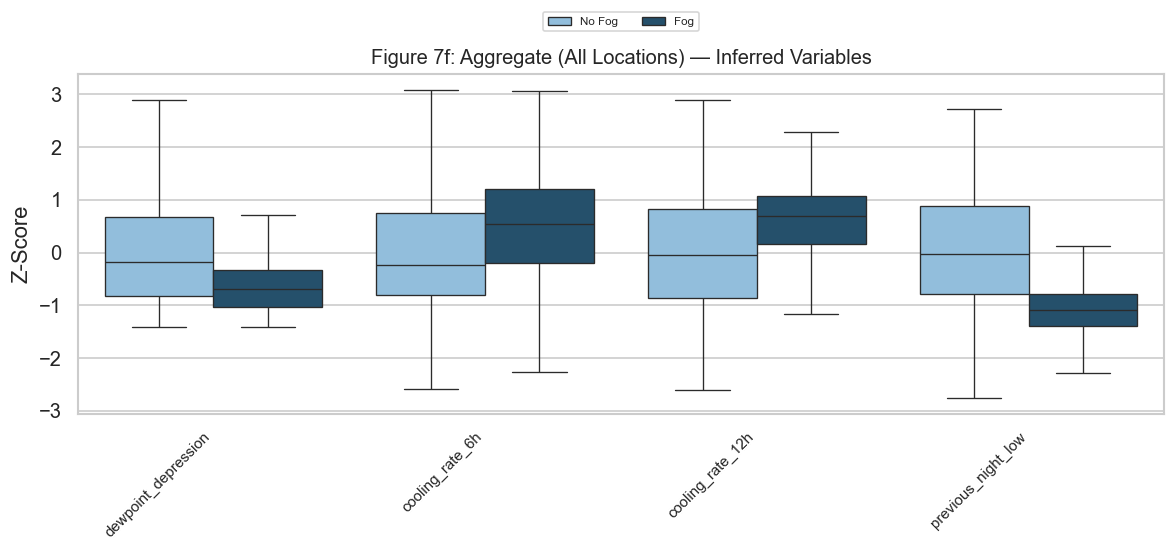
\includegraphics[keepaspectratio]{report_files/figure-pdf/cell-12-output-7.png}}

The box plot distributions for the inferred variables show good
agreement with theoretical expectations for the formation of radiation
fog. This proves the effectiveness of the engineered features. As
expected, the dewpoint depression for the fog conditions is
significantly lower compared to the non-fog conditions for all the
locations. Furthermore, the dewpoint depression results show saturated
air masses that are favorable for condensation processes. The
significant difference between the fog and non-fog conditions for this
variable proves the dominance of the predictor for the presence of fog
since the basic requirement for the formation of fog is for the relative
humidity to approach 100\%.

The cooling rate variables also show the expected distributional
characteristics, with fog events having more negative values for both
6-hour and 12-hour cooling rates. More negative values in this case
reflect efficient nocturnal radiative cooling that acts to decrease the
air temperature to a dew point and thereby produce fog under clear-sky
and calm conditions. The consistency in the sign of these differences
across locations serves to reinforce the physical relevance of cooling
rate as a predictor for fog and illustrates the benefits that come from
including temporal temperature evolution in the feature set. Similarly,
lower values for low temperature from the previous night are observed
during fog events due to the fact that fog often lingers from overnight
formation into the morning hours and that lower overnight low
temperatures are associated with more efficient radiative cooling and
greater probability for saturation.

These findings verify the presence of the inferred variables as
important mechanistic aspects of the development of radiation fog beyond
the information contained in instantaneous weather data. The significant
separation observed in the fog and non-fog distributions implies that
the engineered features are expected to contribute significantly to the
performance of the model and may perform better than the raw weather
data in terms of prediction potential, despite being based on the same
temperature and humidity data.

\subsection{K-Means Sensitivity
Analysis}\label{k-means-sensitivity-analysis}

To further evaluate the impact of AQI features on the underlying
structure of the data, an unsupervised k-means analysis was conducted
with \(k = 8\) clusters (optimized \(k = n\) via elbow method). This
analysis quantifies how the addition or removal of AQI features affects
feature importance and dataset homogeneity.

K-means partitions the data into \(k\) clusters by minimizing the
within-cluster sum of squares (inertia):

\[\text{Inertia} = \sum_{i=1}^{k} \sum_{\mathbf{x} \in C_i} \|\mathbf{x} - \boldsymbol{\mu}_i\|^2\]

where \(C_i\) is cluster \(i\) and \(\boldsymbol{\mu}_i\) is its
centroid.

\begin{itemize}
\tightlist
\item
  \textbf{Silhouette Score}: Measures how similar an observation is to
  its own cluster compared to other clusters. Ranges from -1 to 1, with
  higher values indicating better separation.
\item
  \textbf{Davies-Bouldin Index}: Measures average similarity between
  clusters. Lower values indicate better clustering.
\end{itemize}

For each dataset variant, \textbf{feature variance across clusters} was
calculated to identify which variables contribute most to cluster
separation. This is calculated as the variance of cluster centroids for
each feature, normalized to sum to 100\%.

The analysis was performed separately on each location's three dataset
variants: Without AQI (full), With AQI (filtered + AQI features), and
Without AQI Reduced (filtered, no AQI).

The k-means analysis code can be found in
\texttt{/eda/k-means\ clustering} within the codebase.

\pandocbounded{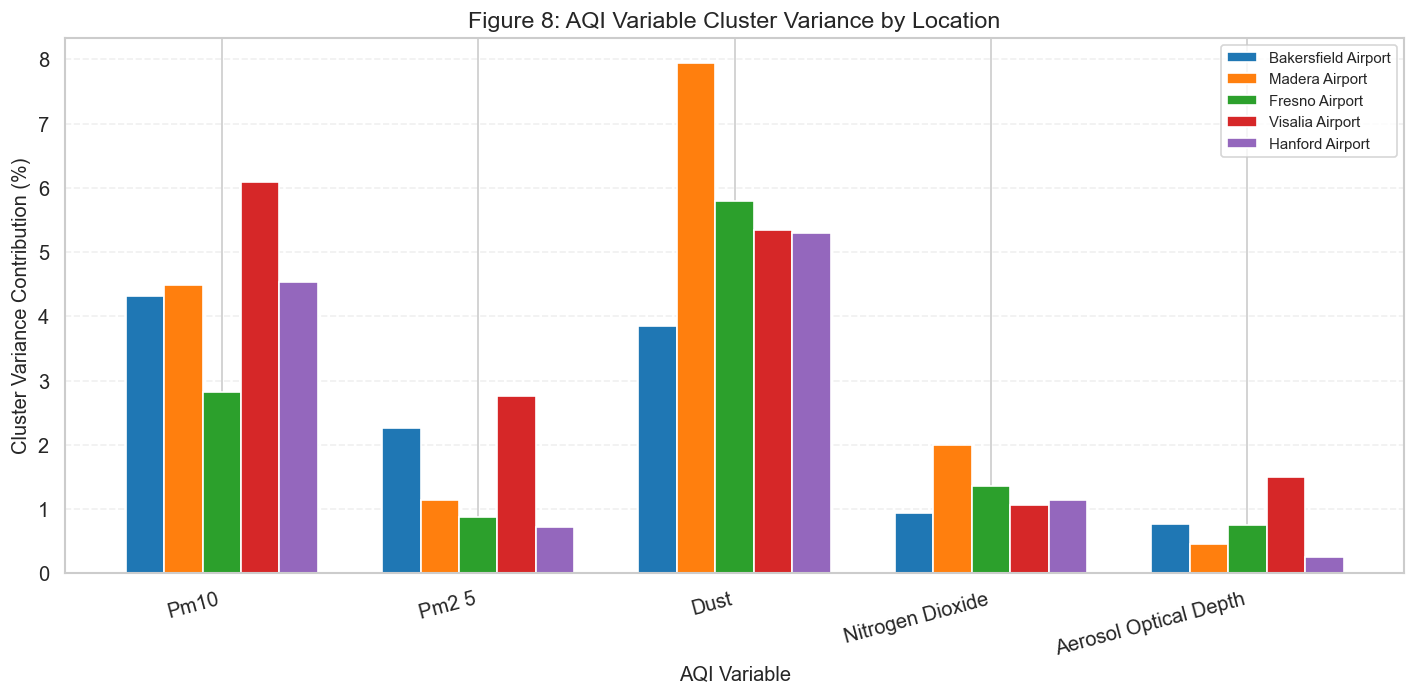
\includegraphics[keepaspectratio]{report_files/figure-pdf/cell-13-output-1.png}}

Dust and PM10 are clearly the dominant factors in contributing to the
variance in the clusters, with the majority of the contributions coming
from these factors on average across the sites. However, the
contribution of these factors is quite variable across the sites. For
Madera, Fresno, Visalia, and Hanford, the contribution of dust is
relatively high, ranging from 5-8\%. In contrast, the contribution of
PM10 is the highest in Bakersfield, with a value of 4.3\%, while the
contribution of dust is relatively low in this location.

On the other hand, PM2.5, nitrogen dioxide, and aerosol optical depth
contribute much less to cluster variance across all locations, ranging
between 1-3\% or lower. These lower variance contributions of finer
particulate matter and gaseous air pollutants indicate that, even though
these air pollutants have stronger correlations with visibility, as
found in previous analyses, these air pollutants do not help define
distinct boundaries between clusters, which is a result of the k-means
clustering process. This difference between stronger correlations with
visibility and lower contributions to defining cluster boundaries
between air quality states indicates that PM2.5 and nitrogen dioxide
vary continuously rather than showing sharp distinctions between air
quality states. The low contribution to cluster variance of aerosol
optical depth across all locations further supports that this
column-integrated aerosol property is not helpful in distinguishing
fog-related air quality states from all other air quality states
included in the 2022-present AQI dataset.

\pandocbounded{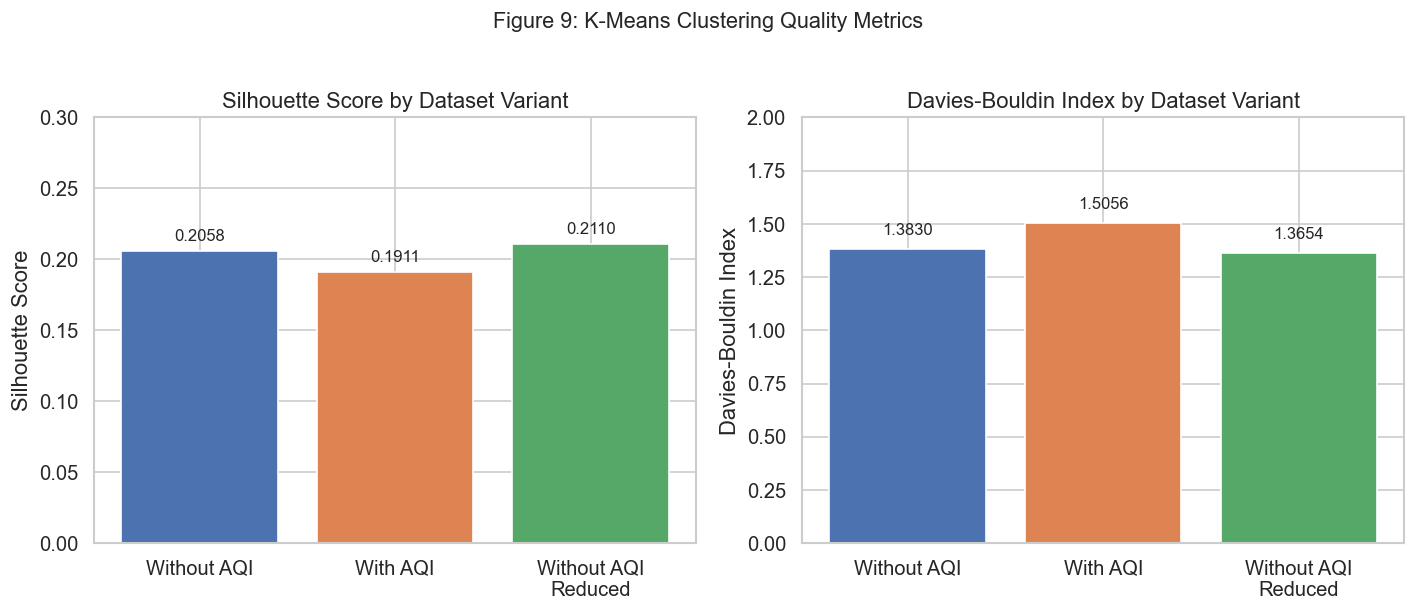
\includegraphics[keepaspectratio]{report_files/figure-pdf/cell-14-output-1.png}}

\pandocbounded{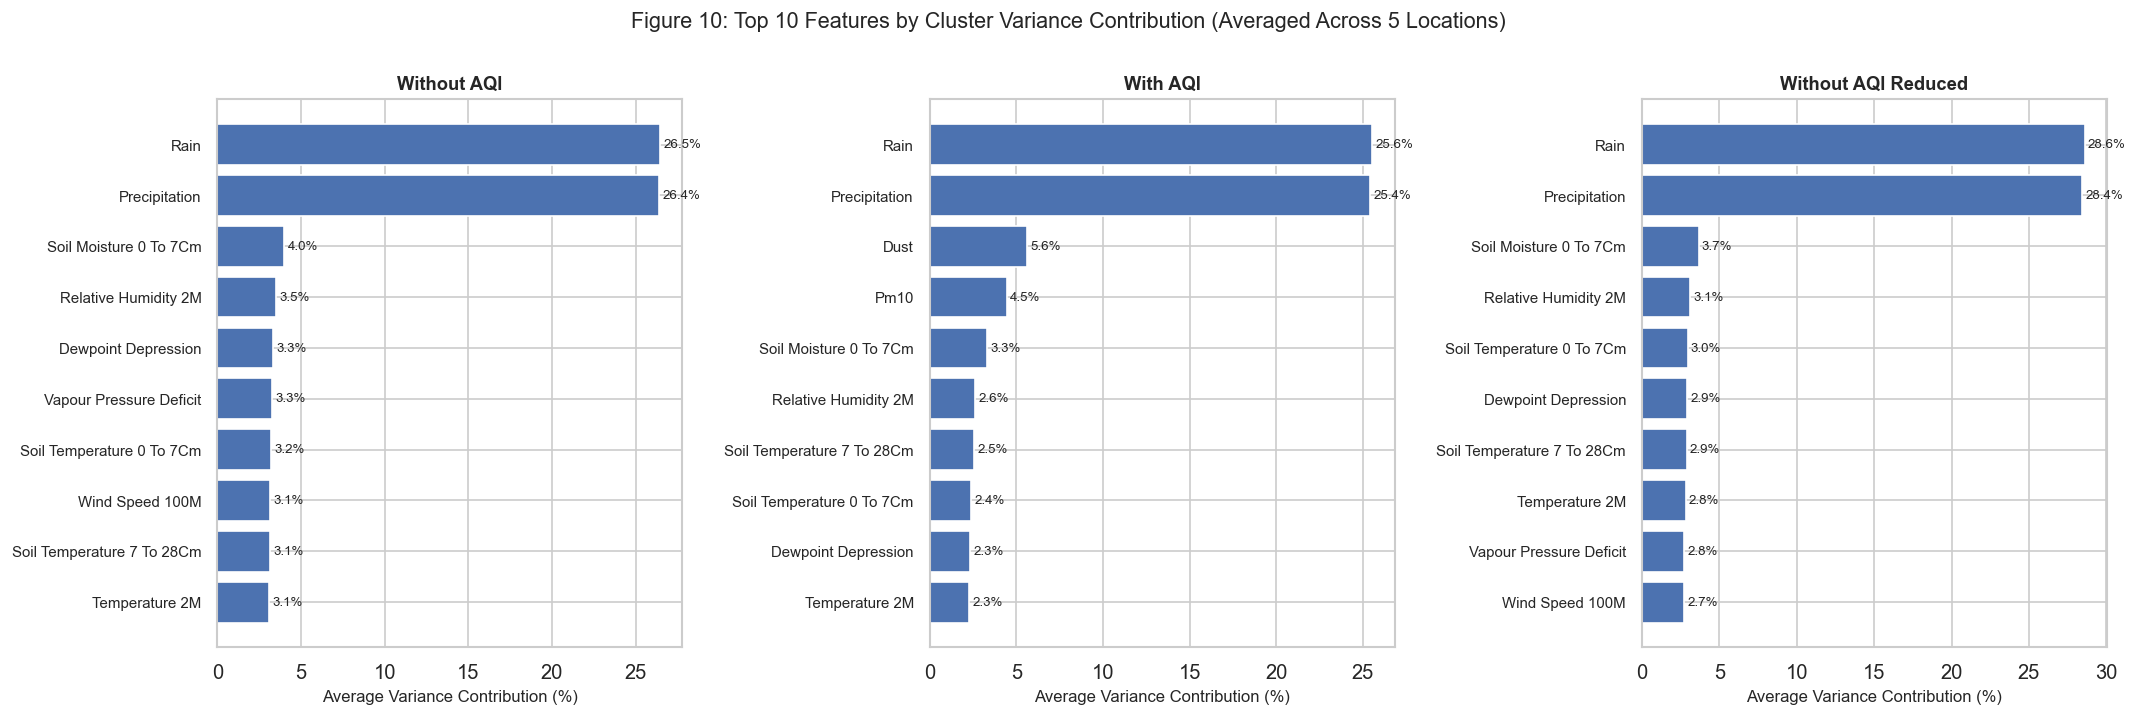
\includegraphics[keepaspectratio]{report_files/figure-pdf/cell-14-output-2.png}}

The clustering quality metrics show that there is a general trend across
variants in which the addition of AQI features negatively impacted the
quality of unsupervised clustering. The \textbf{With AQI} variant has
the lowest Silhouette Score at 0.1911 and highest Davies-Bouldin Index
at 1.5056, which suggests that this variant has clusters that are less
distinct internally and more prone to overlap with neighboring clusters
compared to other variants. On the other hand, the \textbf{Without AQI
Reduced} variant shows a better clustering quality with a Silhouette
Score of 0.2110 and Davies-Bouldin Index of 1.3654. This analysis
specifically targets the effect of AQI features by comparing variants
and demonstrates that AQI features indeed contribute noise and not
meaningful clustering in the atmospheric state space. However, it must
be noted that the \textbf{Without AQI} variant with 15-20 times more
data points and covering 45 years still manages to have a clustering
quality that is in between and competitive with the \textbf{Without AQI
Reduced} variant in terms of Silhouette Scores and Davies-Bouldin
Indices, with a Silhouette Score of 0.2058 and Davies-Bouldin Index of
1.3830.

The feature variance contributions also highlight the dominance of
precipitation-related features in defining cluster boundaries. Across
all three variants of the datasets, rain and precipitation combined
account for 50-60\% of total cluster variance, with individual features
contributing 25-30\%. This is due to the binary nature of rain and
precipitation in the semi-arid environment of the San Joaquin Valley.
Hours with rain or precipitation have categorically different clusters
compared to the vast majority of hours without rain or precipitation,
even as temperature, humidity, pressure, or air quality may vary. The
discrete nature of rainfall leads to natural cluster separations that
dwarf the differences in other meteorological features. The k-means
algorithm is thus seen to partition the data along the
rain/precipitation axis, with a secondary partitioning based on soil
moisture and humidity conditions.

In the presence of features in AQI, dust and PM10 emerge as the third
and fourth most important features in the \textbf{With AQI} variant.
They contribute 5.65\% and 4.45\% to the total variance in the data.
This is much higher than the importance of weather-related features such
as temperature, wind speed, and surface pressure. This indicates that
dust and PM10 are important features in the data. Although dust and PM10
are individually important features in the data, the overall quality of
clustering is reduced in the presence of features in AQI. This indicates
that dust and PM10 define the axes orthogonal to the weather-related
structure in the data relevant for fog classification. This is
consistent with the previous analysis that suggested that features in
AQI have low predictive power for the classification task. This is
because features in AQI contribute to the overall structure in the data
but not to the structure relevant for the classification task.

\section{Methods and Results}\label{methods-and-results}

This section describes each classification model used to predict fog
events and reports comparative performance across dataset variants and
locations. All models were evaluated using a \textbf{temporal train/test
split}: data from \textbf{1980--2023 + 2025} for training and
\textbf{2024} for testing. The year 2024 was selected as the test set to
maintain consistency across all models and establish a fair baseline for
comparison. Given that the AQI-enhanced dataset spans only
\textbf{2022--2025}, and within this window \textbf{only 2023 and 2024
represent complete calendar years}, using 2024 as the held-out test year
ensures that model evaluation captures the full range of seasonal fog
patterns and avoids biases introduced by partial-year data.

Three dataset configurations were tested for each model:

\begin{longtable}[]{@{}
  >{\raggedright\arraybackslash}p{(\linewidth - 6\tabcolsep) * \real{0.2368}}
  >{\raggedright\arraybackslash}p{(\linewidth - 6\tabcolsep) * \real{0.1579}}
  >{\raggedright\arraybackslash}p{(\linewidth - 6\tabcolsep) * \real{0.2632}}
  >{\raggedright\arraybackslash}p{(\linewidth - 6\tabcolsep) * \real{0.3421}}@{}}
\toprule\noalign{}
\begin{minipage}[b]{\linewidth}\raggedright
Variant
\end{minipage} & \begin{minipage}[b]{\linewidth}\raggedright
Rows
\end{minipage} & \begin{minipage}[b]{\linewidth}\raggedright
Features
\end{minipage} & \begin{minipage}[b]{\linewidth}\raggedright
Description
\end{minipage} \\
\midrule\noalign{}
\endhead
\bottomrule\noalign{}
\endlastfoot
\textbf{Without AQI} & ≈ 168-400k & 20 weather & Full 45-year record, no
air quality columns \\
\textbf{With AQI} & ≈ 27k & 25 (weather + AQI) & Restricted to rows with
valid AQI data (Aug 2022+) \\
\textbf{Without AQI Reduced} & ≈ 27k & 20 weather & Same rows as With
AQI, but AQI columns removed (control) \\
\end{longtable}

Fog: \(< 1{,}610\) m (1 mile)

No Fog: Otherwise

Performance metrics reported are \textbf{accuracy}, \textbf{precision},
\textbf{recall}, \textbf{F1-score}, and \textbf{ROC-AUC}, averaged
across five locations.

\textbf{All models and results can be found and re-used within
\texttt{/models} in the codebase.}

\textbf{Appendixes B - G contain raw results, per location, for all
model outputs.}

\subsection{Logistic Regression}\label{logistic-regression}

Logistic Regression models the probability of fog as a sigmoid function
of a linear combination of input features. Given feature vector
\(\mathbf{x} \in \mathbb{R}^d\) with learned weights \(\mathbf{w}\) and
bias \(b\):

\[P(y = 1 \mid \mathbf{x}) = \sigma(\mathbf{w}^T \mathbf{x} + b) = \frac{1}{1 + e^{-(\mathbf{w}^T \mathbf{x} + b)}}\]

The model minimizes the regularized binary cross-entropy loss:

\[\mathcal{L} = -\frac{1}{N} \sum_{i=1}^{N} \left[ y_i \log(\hat{y}_i) + (1 - y_i) \log(1 - \hat{y}_i) \right] + \frac{1}{2C} \|\mathbf{w}\|_2^2\]

where \(C\) is the inverse regularization strength. Features are
standardized via \texttt{StandardScaler} and the
\texttt{class\_weight=\textquotesingle{}balanced\textquotesingle{}}
parameter adjusts the loss to up-weight the minority (fog) class
proportionally. The solver used is L-BFGS with a maximum of 1,000
iterations.

Logistic regression serves as the baseline model for this study due to
its simplicity. Its strength lies in its ability to provide linear
decision boundaries that are easy to interpret, becase each feature's
coefficient directly represents its contribution to the log-odds of fog
occurrence.

However, there are considerable limitations to using logistic
regression, especially with complex weather phenomena such as fog
formation. To start with, logistic regression is a linear method that is
not well suited to handle non-linear relationships between variables,
such as the combined effects of humidity and temperature, or threshold
effects, such as fog formation depending on whether the depression is
above or below a certain critical value. Since fog is known to form
through complex non-linear processes, such as temperature inversion,
radiative cooling, and convergence of moisture, logistic regression may
not effectively identify the complex, high-dimensional patterns that
distinguish fog from near-fog situations. Also, there is considerable
multicollinearity between weather variables such as temperature and
dewpoint, which may affect the performance of logistic regression,
especially if there is class imbalance, despite class weights.

Given these characteristics, it was expected that the logistic
regression algorithm would have low performance success in the task of
predicting fog. It was expected that the algorithm would be successful
in identifying broad trends, such as the strong negative relationship
between visibility and high relative humidity/precipitation, although it
was expected that the algorithm would perform reasonably well in
clear-cut cases in which the atmospheric conditions are clearly
favorable or unfavorable for the occurrence of fog. However, it was
expected that the algorithm would have lower recall compared to
precision, as the algorithm would be unable to detect the occurrence of
fog in nonlinear meteorological conditions.

\pandocbounded{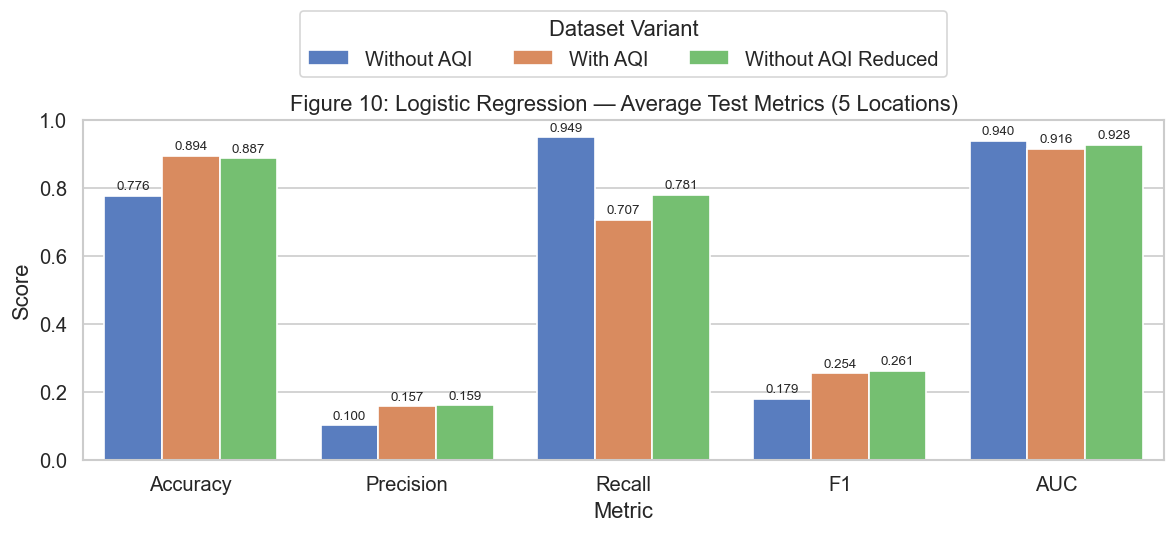
\includegraphics[keepaspectratio]{report_files/figure-pdf/cell-16-output-1.png}}

The logistic regression results reveal performance patterns that
directly reflect the model's fundamental limitations when applied to fog
prediction. Across all three dataset variants, the model exhibits
severely imbalanced precision-recall tradeoffs: precision ranges from
just 10.04\% to 15.92\%, while recall reaches 70.71\% to 94.91\%. This
disparity indicates that the linear decision boundary is unable to
tightly delineate the complex, high-dimensional region where fog
conditions occur. Instead, the model compensates by casting an
excessively wide net and classifying many non-fog hours as fog in order
to capture most actual fog events. The \textbf{Without AQI} variant
demonstrates this effect most dramatically, achieving 94.91\% recall at
the cost of 10.04\% precision, meaning that for every correct fog
prediction, approximately nine false alarms are generated.

This poor precision-recall balance arises from logistic regression's
inability to model the nonlinear interactions and threshold effects that
govern radiation fog formation. The linear model cannot effectively
distinguish between marginal conditions (e.g., high humidity but
insufficient cooling) and true fog-forming scenarios without creating a
decision boundary so conservative that it misses many fog events. The
class imbalance problem exacerbates this issue, as even with balanced
class weights, the model's linear structure limits its capacity to
define a narrow, precise boundary around the minority class.
Consequently, the model sacrifices specificity to maintain sensitivity,
resulting in F1-scores below 0.27 across all variants despite strong AUC
values (0.92--0.94) indicating reasonable rank-ordering ability.

The inclusion of AQI features produces marginal improvements in
precision (+5.6\%) and F1-score (+7.5) compared to the \textbf{Without
AQI} variant, but this comes at the expense of reduced recall (−24.2\%).
This shift suggests that AQI variables introduce some discriminative
signal that helps the model avoid certain false positives, though the
overall precision remains low for operational use. The \textbf{Without
AQI Reduced} variant shows nearly identical performance to \textbf{With
AQI}, confirming that the primary driver of improved precision is the
reduced dataset size and temporal scope (2022--2024) rather than AQI
features themselves. The shorter, more recent time window may contain
fewer edge cases or data anomalies that confused the model trained on 45
years of data.

\subsection{Random Forest}\label{random-forest}

Random Forest constructs an ensemble of \(B\) decision trees, each
trained on a bootstrapped sample. For classification, each tree casts a
vote and the final prediction is determined by majority:

\[\hat{y} = \text{mode}\left\{ h_b(\mathbf{x}) \right\}_{b=1}^{B}\]

Each tree splits nodes by maximizing the Gini impurity reduction:

\[\Delta G = G(\text{parent}) - \sum_{k \in \{\text{left}, \text{right}\}} \frac{n_k}{n} G_k, \quad G = 1 - \sum_{c=1}^{C} p_c^2\]

The model uses \(B = 500\) trees, \texttt{max\_depth=10}, and
\texttt{class\_weight=\textquotesingle{}balanced\textquotesingle{}}. An
F1-optimized probability threshold (searched over 0.01--0.50) replaces
the default 0.5 cutoff.

Random Forestleverages an ensemble of decision trees to capture
nonlinear relationships and complex feature interactions inherent to fog
formation. Its primary strength lies in its ability to automatically
discover threshold effects and interaction terms without explicit
feature engineering. The ensemble structure provides robustness through
variance reduction: by averaging predictions across hundreds of trees
trained on bootstrapped samples with random feature subsets, the model
mitigates overfitting and reduces sensitivity to individual noisy
observations or outliers in the 45-year weather record. Additionally,
Random Forest handles class imbalance more effectively than single
models when combined with balanced class weights, as different trees in
the ensemble can specialize in different regions of the feature space,
allowing some to focus on rare fog events while others model the
dominant clear-weather patterns.

However, Random Forest has notable limitations that may constrain its
effectiveness for fog prediction. The model lacks temporal awareness
since each hourly observation is treated independently, ignoring the
sequential nature of atmospheric evolution leading up to fog formation.
This temporal blindness means the model cannot directly learn that fog
often follows a specific progression of conditions, potentially missing
fog events that arise from dynamic processes rather than instantaneous
snapshots. Furthermore, the fixed tree depth represents a tradeoff
between model capacity and overfitting risk. While shallower trees
prevent memorization of useless patterns in the training data, they may
also limit the model's ability to capture highly intricate,
multi-condition rules that characterize fog formation in diverse
microclimates across the five airports. The bagging procedure and random
feature sampling introduce additional variance that can reduce precision
if the most discriminative features are occasionally excluded from
critical splits.

Given these characteristics, it was expected for Random Forest to
substantially outperform logistic regression by providing a better
precision-recall tradeoff. The model should be able to identify
nonlinear thresholds (e.g., critical values for dewpoint depression) and
interaction effects (e.g., the combined effect of low temperature and
high humidity), resulting in high precision while maintaining or
slightly decreasing recall compared to logistic regression. However, it
was not expected for Random Forest to have achieved an operationally
viable performance for this task, as the failure to account for time
dependencies means that the model cannot exploit the leading indicators
present in the atmospheric signal prior to fog formation.

\pandocbounded{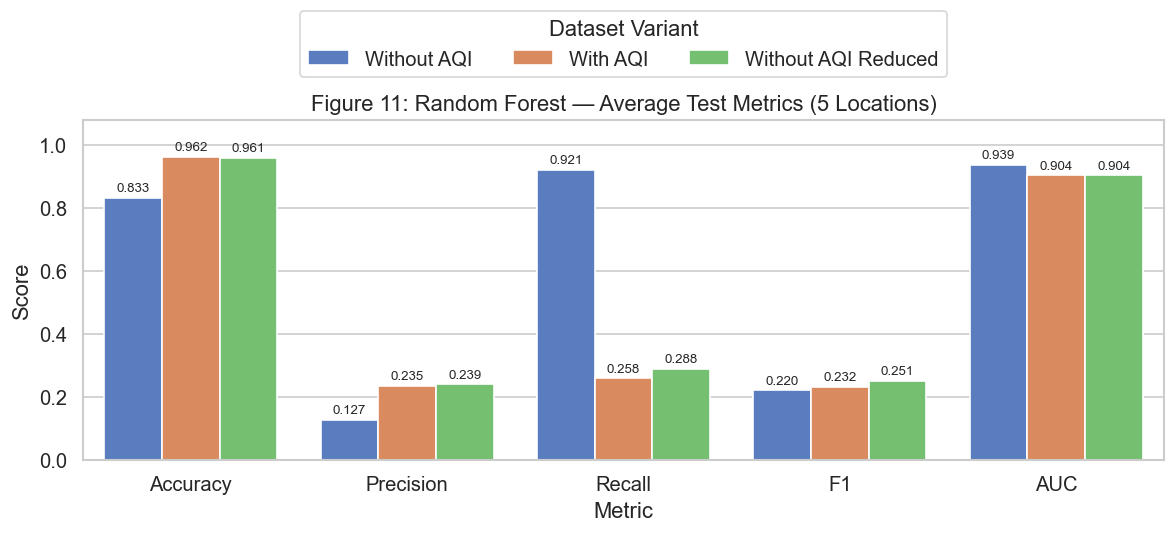
\includegraphics[keepaspectratio]{report_files/figure-pdf/cell-17-output-1.png}}

The Random Forest results demonstrate improvements over logistic
regression in precision, but reveal the model's inability to incorporate
temporal context. The \textbf{Without AQI} variant achieves 12.68\%
precision and 92.13\% recall. This is a minor improvement in precision
(+2.6\%) over logistic regression while maintaining comparably high
recall. However, the \textbf{With AQI} and \textbf{Without AQI Reduced}
variants exhibit a dramatic behavioral shift: precision nearly doubles
to 23\%.48\% and 23.90\% respectively, but recall collapses to just
25.78\% and 28.78\%. This indicates that Random Forest, when trained on
the smaller 2022--2024 dataset, adopts a far more conservative decision
boundary that sacrifices sensitivity for specificity and thereby misses
approximately 70--75\% of fog events to reduce false positives. The
result of this tradeoff are F1-scores (0.22--0.25) that fail to
substantially exceed logistic regression, despite Random Forest's
capacity for nonlinear modeling.

This performance stems from Random Forest's lack of temporal awareness.
Fog formation is inherently a dynamic process characterized by gradual
atmospheric evolution, such as nocturnal cooling, gradual humidity
increases, and wind speed decreases. By treating each hourly observation
as independent, Random Forest cannot learn these sequential precursor
signals. Instead, it must rely solely on instantaneous snapshots of
atmospheric conditions, many of which are ambiguous when considered in
isolation. For instance, an hour with 90\% relative humidity and 2°C
dewpoint depression might represent an imminent fog event if preceded by
sustained cooling and moisture accumulation, or a transient state that
quickly dissipates if followed by increasing temperatures or winds.
Without access to temporal context, the model cannot distinguish between
these scenarios, forcing it to either overpredict (high recall, low
precision) or underpredict (low recall, high precision) depending on the
decision threshold and dataset characteristics.

The dramatic precision-recall shift between the \textbf{Without AQI}
variant and the \textbf{AQI-inclusive variants} further illustrates this
limitation. The shorter time period likely contains fewer marginal or
ambiguous cases---perhaps due to reduced climatic variability or data
collection improvements in recent years, therefore allowing Random
Forest to adopt a more selective threshold without catastrophically
sacrificing recall. However, even with this advantage, the model still
misses 70\% of fog events in the \textbf{With AQI} variant, suggesting
that instantaneous meteorological features alone are insufficient to
precisely characterize fog formation. The nearly identical performance
between \textbf{With AQI} (F1 = 0.2317) and \textbf{Without AQI Reduced}
(F1 = 0.2511) confirms that AQI features provide minimal additional
predictive power beyond what is already captured by weather variables,
reinforcing earlier exploratory findings.

\subsection{XGBoost}\label{xgboost}

XGBoost (eXtreme Gradient Boosting) builds an additive ensemble of
regression trees, where each new tree \(f_t\) minimizes a regularized
objective:

\[\mathcal{L}^{(t)} = \sum_{i=1}^{N} l\left(y_i, \hat{y}_i^{(t-1)} + f_t(\mathbf{x}_i)\right) + \Omega(f_t)\]

\[\Omega(f) = \gamma T + \frac{1}{2} \lambda \sum_{j=1}^{T} w_j^2\]

where \(T\) is the number of leaves, \(w_j\) are leaf weights, and
\(\gamma\), \(\lambda\) are regularization parameters. A second-order
Taylor expansion of the loss yields optimal leaf weights:

\[w_j^* = -\frac{\sum_{i \in I_j} g_i}{\sum_{i \in I_j} h_i + \lambda}\]

where \(g_i\) and \(h_i\) are the first and second derivatives of the
loss at each sample.

Configuration: - \texttt{n\_estimators=10000} - \texttt{max\_depth=5} -
\texttt{learning\_rate=0.05} - \texttt{early\_stopping\_rounds=1000} -
\texttt{scale\_pos\_weight} - \texttt{+F1\ optimized\ threshold}

XGBoost is a refinement of the Random Forest approach through gradient
boosting, where trees are added sequentially to correct errors made by
previous iterations rather than being trained independently. This
iterative error-correction mechanism is XGBoost's primary strength: each
new tree focuses on the residuals (misclassified or poorly predicted
instances) from the ensemble built so far, allowing the model to
progressively refine decision boundaries in regions of feature space
where classification is most difficult. For fog prediction, this means
XGBoost can allocate modeling capacity to the challenging marginal cases
rather than repeatedly modeling the easy, clear-cut distinctions that
Random Forest's bagging approach may redundantly capture across many
trees. Additionally, XGBoost's second-order gradient optimization and
sophisticated regularization (\(\gamma\), \(\lambda\)) provide
fine-grained control over model complexity, enabling deeper learning of
intricate meteorological patterns while mitigating overfitting through
early stopping and penalization of overly complex trees.

However, XGBoost shares Random Forest's fundamental limitation: it lacks
temporal awareness and treats each hourly observation as independent.
While the boosting mechanism allows for more precise decision boundaries
than bagging, it does not enable the model to learn sequential
atmospheric evolution patterns. Although XGBoost's regularization and
early stopping mitigate this risk, the shallow tree depth and
conservative learning rate represent necessary compromises that may
limit the model's ability to capture extremely complex, high-order
feature interactions. The sequential nature of boosting also makes
XGBoost more sensitive to class imbalance than Random Forest.
Specifically, if early trees in the sequence consistently underpredict
the minority fog class, later trees inherit this bias and may struggle
to recover despite the usage of \texttt{scale\_pos\_weight} adjustments.

Given these characteristics, it was expected that XGBoost outperforms
both logistic regression and Random Forest by achieving the best
precision-recall balance among the non-temporal models. The iterative
refinement should yield higher precision while maintaining reasonable
recall, resulting in F1-scores improvements. It was theorized that
XGBoost would particularly excel in the \textbf{Without AQI} variant
where the large 45-year dataset provides ample training signal for the
boosting process to refine decision boundaries, while performance may
degrade slightly in the \textbf{AQI-inclusive} variants where the
smaller sample size limits the benefit of iterative error correction.

\pandocbounded{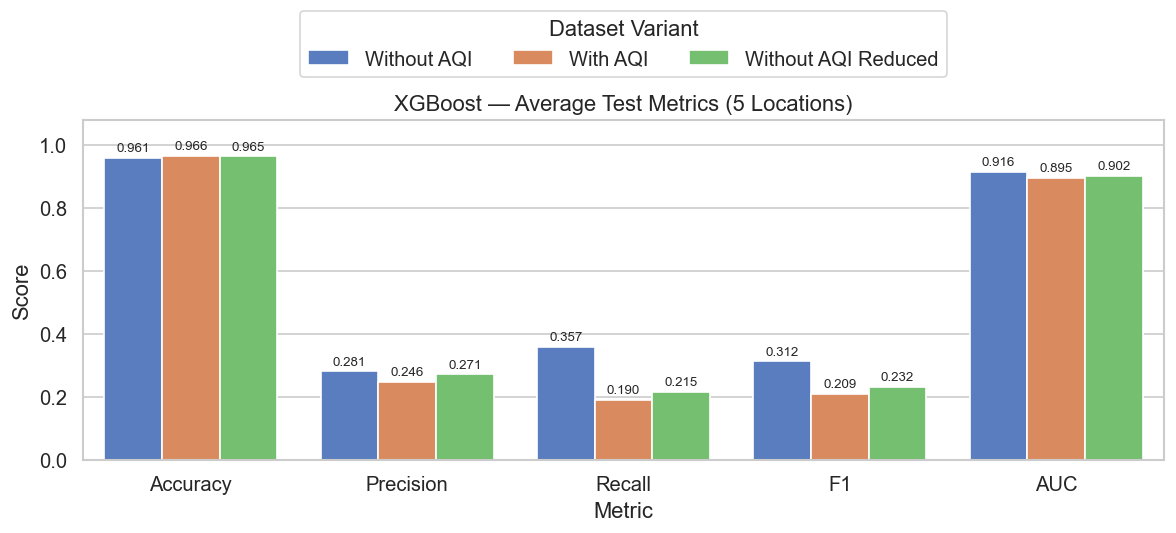
\includegraphics[keepaspectratio]{report_files/figure-pdf/cell-18-output-1.png}}

XGBoost delivers the strongest performance among the non-temporal models
as expected, achieving the best precision-recall balance and the highest
F1-score across most variants. The \textbf{Without AQI} variant
demonstrates this most clearly: 28.07\% precision and 35.72\% recall
yield an F1-score of 0.3120, outperforming both logistic regression (F1
= 0.1793) and Random Forest (F1 = 0.2201). This improvement confirms
that gradient boosting's iterative error-correction mechanism
successfully refines decision boundaries in the challenging regions of
feature space where atmospheric conditions are ambiguous. By
progressively focusing on misclassified fog events and near-miss
predictions, XGBoost learns more nuanced decision rules than Random
Forest's independent trees or logistic regression's linear boundary,
resulting in fewer false positives.

However, XGBoost's performance degrades significantly when applied to
the AQI-inclusive datasets, revealing the model's shared limitation with
other non-temporal approaches: inability to leverage sequential
atmospheric evolution. The \textbf{With AQI} variant exhibits 24.65\%
precision and only 18.95\% recall (F1 = 0.2091). This is worse than the
\textbf{Without AQI} variant despite having access to five additional
air quality features. This counterintuitive degradation arises from two
factors. First, the much smaller training dataset provides insufficient
examples for gradient boosting's iterative refinement to converge on
robust decision boundaries, particularly for the rare fog class. Second,
the AQI features introduce orthogonal variance that is not aligned with
fog-relevant atmospheric structure (shown in k-means analysis), dust and
PM10 capture substantial data variance but along dimensions that do not
necessarily discriminate between fog and non-fog conditions. XGBoost's
boosting process may overfit to these patterns in the limited training
data, leading to decision rules that generalize poorly to the 2024 test
set.

The \textbf{Without AQI Reduced} variant provides a controlled
comparison that isolates the dataset size effect: with 27.07\%
precision, 21.52\% recall, and F1 = 0.2321, this variant performs
slightly better than \textbf{With AQI} but still worse than
\textbf{Without AQI}. This confirms that the smaller temporal window
(2022--2024) is the primary driver of performance degradation, not the
AQI features themselves. The shorter time period offers fewer training
examples and likely less climatic diversity limiting XGBoost's ability
to learn generalizable fog formation patterns. Even with the best
performance in the \textbf{Without AQI} variant, XGBoost still misses
nearly two-thirds of fog events (recall 35.72\%), demonstrating that
instantaneous meteorological snapshots, regardless of how they are
modeled through gradient boosting, are insufficient to fully
characterize fog occurrence. Fog formation depends on temporal
trajectories of cooling, moisture accumulation, and wind decay over
preceding hours.

\subsection{Temporal Convolutional Neural
Network}\label{temporal-convolutional-neural-network}

The Temporal CNN processes sequences of \(L = 24\) consecutive hourly
observations to capture atmospheric evolution patterns leading to fog
formation. Each input is a matrix
\(\mathbf{X} \in \mathbb{R}^{L \times d}\) where \(d\) is the number of
features. The architecture consists of three 1D convolutional blocks
with progressively increasing filter counts, followed by global max
pooling and two fully connected layers:

\textbf{Convolutional Blocks:} Each block applies 1D convolution, batch
normalization, and pooling with dropout:

\[\mathbf{z}_l^{(k)} = \text{Dropout}\left(\text{Pool}\left(\text{ReLU}\left(\text{BN}\left(\mathbf{W}^{(k)} * \mathbf{z}_{l-1} + \mathbf{b}^{(k)}\right)\right)\right)\right)\]

where \(*\) denotes 1D convolution with kernel size 3 and \texttt{same}
padding. The filter counts are 64, 128, and 256 for \(k = 1, 2, 3\)
respectively. The first two blocks use MaxPooling1D(2) while the third
uses GlobalMaxPooling1D to extract the most salient temporal features.

\textbf{Dense Layers:} After global pooling, two fully connected layers
with L2 regularization refine the representation:

\[\mathbf{h}_1 = \text{Dropout}_{0.55}\left(\text{BN}\left(\text{ReLU}(\mathbf{W}_1 \mathbf{h}_0 + \mathbf{b}_1)\right)\right), \quad \mathbf{W}_1 \in \mathbb{R}^{128 \times 256}\]

\[\mathbf{h}_2 = \text{Dropout}_{0.5}\left(\text{BN}\left(\text{ReLU}(\mathbf{W}_2 \mathbf{h}_1 + \mathbf{b}_2)\right)\right), \quad \mathbf{W}_2 \in \mathbb{R}^{64 \times 128}\]

\[\hat{y} = \sigma(\mathbf{W}_o \mathbf{h}_2 + b_o)\]

Both dense layers use L2 regularization with \(\lambda = 0.01\):
\(\Omega(\mathbf{W}) = 0.01 \|\mathbf{W}\|_2^2\). The model is trained
for up to 50 epochs using the Adam optimizer (learning rate 0.001),
binary cross-entropy loss, class weights inversely proportional to class
frequencies, and early stopping with patience 10 on validation loss.

The Temporal CNN's fundamental strength lies in its ability to model the
sequential atmospheric evolution that precedes fog formation. By
processing 24-hour lookback windows, the network can learn temporal
patterns such as sustained nocturnal cooling, gradual moisture
accumulation, and persistent calm wind conditions that collectively
signal fog onset. The 1D convolutional filters act as learnable temporal
pattern detectors: early layers capture short-range features like
hour-to-hour temperature changes or humidity fluctuations, while deeper
layers with larger receptive fields integrate these into longer-range
patterns that span multiple hours. This hierarchical temporal feature
extraction allows the model to distinguish between transient atmospheric
states and sustained conditions that lead to fog. Additionally, the
architecture's use of batch normalization, dropout (0.5-0.55), and L2
regularization provides strong regularization to prevent overfitting on
the 45-year dataset's historical idiosyncrasies.

However, the Temporal CNN faces significant challenges related to data
imbalance, sequence construction limitations, and model complexity. The
fixed 24-hour window represents a rigid assumption about the timescale
of fog formation: some fog events may develop on shorter timescales
(e.g., 6-12 hours of rapid cooling) while others may require longer
contextual windows (e.g., multi-day synoptic patterns). The architecture
cannot adaptively adjust its temporal receptivity to different fog
formation scenarios. The model's deep structure (3 convolutional blocks
+ 2 dense layers) also introduces substantial parameters
(\textasciitilde500k-1M depending on input dimensions) that must be
learned from a limited number of fog sequences, increasing the risk of
overfitting despite regularization. The max pooling operations, while
providing translation invariance and computational efficiency, discard
temporal position information that may be relevant. For example, if peak
humidity occurs at midnight versus 4am could be diagnostic of fog
timing.

Nonetheless, it was expected that the Temporal CNN outperforms all other
models by leveraging sequential atmospheric signals, but the degree of
improvement may be constrained by class imbalance and sequence
construction challenges. Improved recall compared to XGBoost was
expected as the model learned to recognize the temporal precursor
patterns that consistently precede fog formation, though precision may
remain modest due to high class imbalance in the datasets. On the other
hand, F1-scores should represent meaningful progress over non-temporal
baselines, particularly if recall improves substantially. Performance on
the \textbf{Without AQI} variant should theoretically be strongest due
to the large 45-year training set providing diverse examples of
fog-forming sequences across different seasons and climatic conditions.

\pandocbounded{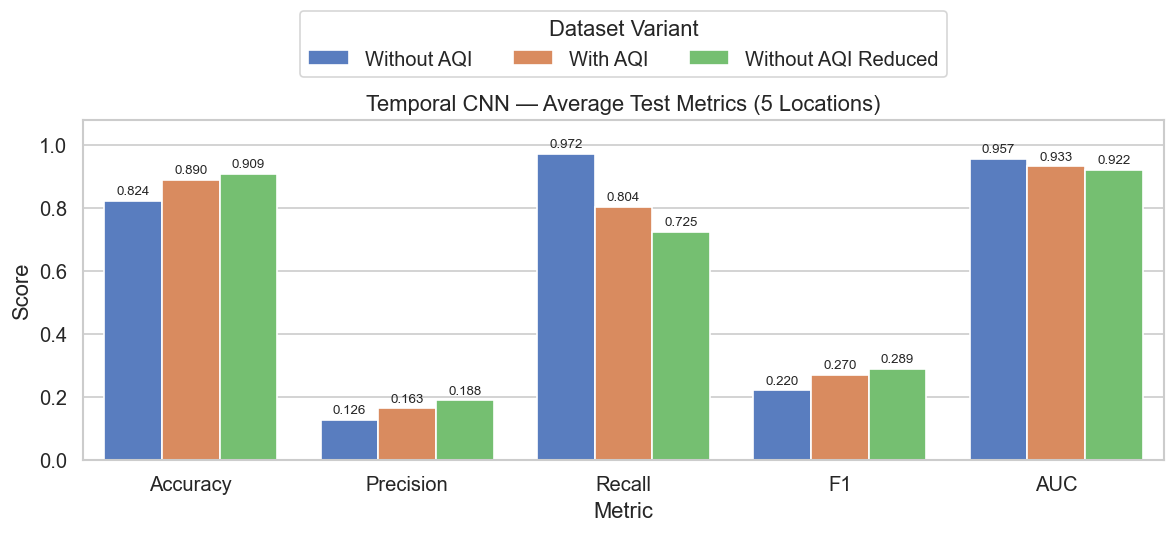
\includegraphics[keepaspectratio]{report_files/figure-pdf/cell-19-output-1.png}}

The Temporal CNN results reveal a mixed outcome: despite having explicit
access to 24-hour atmospheric evolution sequences, the model fails to
translate this temporal awareness into improved classification
performance relative to simpler, non-temporal approaches. The
\textbf{Without AQI} variant exhibits 97.22\% recall paired with only
12.61\% precision, yielding an F1-score of 0.2201. This is identical to
Random Forest and only marginally better than logistic regression (F1 =
0.1793). This extreme recall-precision imbalance mirrors the behavior of
logistic regression from the baseline analysis, indicating that the
Temporal CNN has adopted a similarly aggressive decision threshold that
classifies a vast majority of ambiguous hours as fog in order to capture
nearly all true fog events. For every correct fog prediction, the model
generates approximately 7-8 false alarms.

This performance directly \textbf{reflects the model's struggle with the
severe class imbalance problem}. With fog events representing
\textless5\% of observations, the training signal appears to be too
sparse for the Temporal CNN to adequately outperform other approaches.
The model's response with 97\% recall and 13\% precision suggests it
learned to recognize broad atmospheric patterns associated with fog
formation (high humidity, low temperature, calm winds sustained over
multiple hours) but failed to learn the subtle distinctions that
separate true fog-forming sequences from similar-but-non-fog sequences.
The high AUC (0.9567) confirms that the model produces well-calibrated
probability scores that correctly rank fog events higher than non-fog
events, but the poor precision indicates the model's probability
threshold cannot be adjusted to achieve acceptable specificity without
sacrificing sensitivity.

The performance trends across dataset variants further expose the
model's limitations. The \textbf{With AQI} variant shows improved
precision (16.29\%) but reduced recall (80.39\%, F1 = 0.2697), while the
\textbf{Without AQI Reduced} variant continues this pattern (18.78\%
precision, 72.48\% recall, F1 = 0.2894). These results suggest that the
smaller 2022-2024 dataset, while containing fewer training sequences
overall, may present less ambiguous cases or benefit from more
consistent modern data collection practices, allowing the model to adopt
a more selective threshold. However, even the best F1-score (0.2894)
barely exceeds logistic regression's performance on the same data (F1 =
0.2605) and falls well of XGBoost's \textbf{Without AQI} performance (F1
= 0.3120). This reveals that the theoretical advantage of temporal
modeling is largely negated in practice by the compound challenges of
extreme class imbalance and thus the model's inability to learn
sufficiently discriminative temporal patterns from such an intensely
sparse training signal.

\subsection{Sequential Stacking
Ensemble}\label{sequential-stacking-ensemble}

The ensemble combines all four base models in a sequential stacking
architecture where each layer augments the input for the next:

\textbf{Layer 1 --- Logistic Regression:} Trained on standardized
features. Produces probability \(p_1 = P_{\text{LR}}(\mathbf{x})\).

\textbf{Layer 2 --- Random Forest:} Trained on original features
concatenated with \(p_1\). Produces
\(p_2 = P_{\text{RF}}(\mathbf{x} \| p_1)\).

\textbf{Layer 3 --- XGBoost:} Trained on original features concatenated
with \(p_1\) and \(p_2\). Produces
\(p_3 = P_{\text{XGB}}(\mathbf{x} \| p_1 \| p_2)\).

\textbf{Layer 4 --- Temporal CNN:} Trained on standardized features
concatenated with \(p_1\), \(p_2\), and \(p_3\), reshaped into 24-step
sequences. Produces
\(p_4 = P_{\text{CNN}}(\mathbf{X}_{24} \| p_1 \| p_2 \| p_3)\).

The final prediction is a weighted average:

\[\hat{p} = 0.10 \cdot p_1 + 0.20 \cdot p_2 + 0.30 \cdot p_3 + 0.40 \cdot p_4\]

An F1-optimized threshold \(\tau^*\) converts \(\hat{p}\) to binary
predictions:

\[\hat{y} = \mathbb{1}[\hat{p} \geq \tau^*], \quad \tau^* = \arg\max_{\tau \in [0.01, 0.50]} F_1(\tau)\]

The stacking ensemble's fundamental strength lies in its ability to
synthesize complementary modeling perspectives through a hierarchical
architecture that progressively enriches the feature representation at
each layer. By allowing later models to condition on the predictions of
earlier models, the ensemble creates opportunities for deep error
correction and pattern refinement that single models are unable to
achieve. Logistic regression provides a simple, interpretable baseline
that captures linear relationships; Random Forest adds the predictions
from this linear perspective as a meta-feature while introducing
nonlinear decision boundaries through its tree ensemble; XGBoost refines
these boundaries by accessing both the logistic and Random Forest
predictions; finally, the Temporal CNN integrates all three prior
predictions along with the full 24-hour temporal context, potentially
learning to weight different base models differently depending on
atmospheric evolution patterns. The weighted averaging scheme
(10\%-20\%-30\%-40\%) explicitly encodes a preference for more
sophisticated models while preventing any single component from
dominating, providing regularization through model diversity.

However, the ensemble faces significant challenges related to error
propagation, complexity, and the fundamental data limitations that
constrained individual models. The sequential architecture creates a
dependency chain where errors from early layers compound through
subsequent stages: if logistic regression consistently overpredicts fog
(as observed, with 95\% recall and 10\% precision), its noisy
probability estimates become input features for Random Forest,
potentially misleading the tree-building process. Similarly, if both
logistic regression and Random Forest produce overconfident predictions
in ambiguous regions of feature space, XGBoost inherits a biased
representation that may be difficult to correct through gradient
boosting alone. The Temporal CNN, positioned at the final layer, must
somehow untangle these accumulated errors while simultaneously
processing 24-hour sequences. The fixed weighting scheme
(10\%-20\%-30\%-40\%) represents a manual design choice rather than a
learned meta-model, potentially suboptimal if the relative strengths of
base models vary across different atmospheric conditions or locations.
Most importantly, the ensemble cannot overcome the fundamental class
imbalance and sparse fog signal that plagued individual models: stacking
provides new perspectives on existing data but does not generate new
training signal for the minority fog class.

Given these characteristics, it was expected that the stacking ensemble
acieves the best overall performance across all models by successfully
combining each component's strengths while mitigating weaknesses through
diversification. The ensemble should achieve better precision-recall
balance than individual models by leveraging XGBoost's precise
boundaries to reduce false positives while relying on the Temporal CNN's
high sensitivity to maintain detection of complex fog events. The
strongest performance should occur in the \textbf{Without AQI} variant
where the large 45-year dataset provides robust training for all base
models, while AQI-inclusive variants may show degraded performance as
individual model weaknesses (particularly XGBoost's struggle with small
datasets and the CNN's precision issues) propagate through the stacking
layers. However, it is not anticipated that the ensemble to deliver
transformative performance beyond the 0.40 F1-score ceiling, as the
fundamental challenges of an insufficiently strong signal impose a hard
performance ceiling that no combination of models can overcome.

\pandocbounded{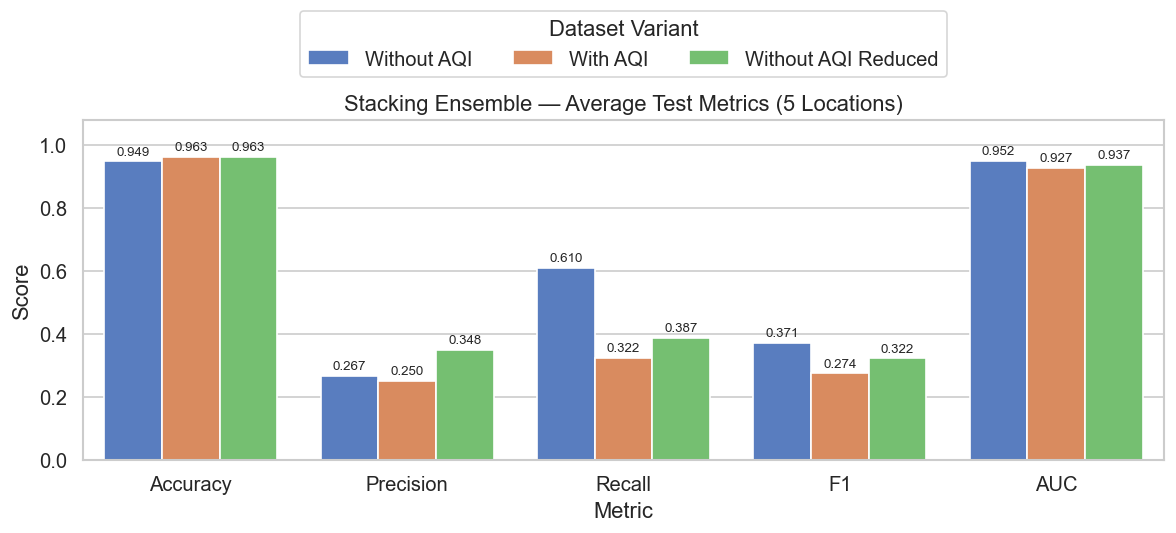
\includegraphics[keepaspectratio]{report_files/figure-pdf/cell-20-output-1.png}}

The stacking ensemble achieves the strongest overall performance of all
models, confirming that multi-model synthesis provides meaningful value
beyond individual approaches. The \textbf{Without AQI} variant delivers
F1 = 0.3706 with 26.68\% precision and 61.04\% recall, which vastly
exceeds XGBoost's standalone result (F1 = 0.3120, precision 28.07\%,
recall 35.72\%) and doubling the logistic regression baseline (F1 =
0.1793). This improvement demonstrates that the hierarchical stacking
architecture successfully leverages complementary strengths: XGBoost
contributes precise decision boundaries that reduce false positives,
while the Temporal CNN's high sensitivity (97\% recall standalone) helps
maintain fog detection coverage, and the intermediate models provide
regularization through diversity. The 61\% recall represents a practical
compromise. Detection of roughly three-fifths of fog events while
generating approximately 2.7 false alarms per correct prediction (down
from XGBoost's 2.6 but far better than the CNN's \textasciitilde7.9)
places this hybrid approach as the best-fit candidate for further
development. The strong AUC (0.9515) confirms good probability
calibration across the full range of atmospheric conditions.

However, the ensemble's performance continues to reflect the challenges
presented by the sparse minority fog class. First, the precision ceiling
of 27\% remains operationally problematic: even with sophisticated
multi-model fusion, the system cannot reliably distinguish fog-forming
conditions from superficially similar atmospheric states, generating
roughly three false alarms for every correct detection. This suggests
that the hourly meteorological features themselves contain insufficient
signal to precisely characterize fog occurrence at the time of
prediction. Second, the \textbf{With AQI} variant exhibits dramatic
performance degradation (F1 = 0.2742), falling below even XGBoost's
standalone performance on the same data (F1 = 0.2091 for XGBoost With
AQI, though note XGBoost Without AQI was 0.3120). This result indicates
error propagation through the stacking layers: the small 2.5-year AQI
dataset causes individual base models to produce noisy, overconfident
predictions that mislead subsequent layers, with errors compounding
through the sequential architecture. The Temporal CNN at the final layer
then inherits these corrupted probability estimates and fails to
untangle them.

ON the other hand, the \textbf{Without AQI Reduced} variant demonstrates
the ensemble's best precision (34.77\%) though with modest recall
(38.73\%, F1 = 0.3218). This pattern of higher precision achieved
through the same stacking architecture suggests that when base models
are trained on cleaner, more recent data (2022-2024) they produce more
reliable probability estimates that the ensemble can effectively
synthesize. The improved precision indicates fewer false alarms (roughly
1.9 per correct detection versus 2.7 for Without AQI), though this comes
at the cost of missing 61\% of fog events. The tradeoff reflects the
fundamental tension in fog prediction: atmospheric conditions can be
ambiguous even with perfect data, and the model must choose between
casting a wide net (high recall, many false positives) or being
selective (high precision, many missed events). In the context of this
problem where missed events can result in catastrophic outcomes,
prioritization of models with high recall, such as the standalone CNN,
emerge as the better choice in practical usage.

Overall, the stacking ensemble results establish the practical
performance ceiling for conventional machine learning approaches on this
fog prediction task: F1-scores around 0.35-0.37 with precision 27-35\%
and recall 39-61\% depending on dataset characteristics and
precision-recall preference. These results represent meaningful progress
over simpler baselines (reducing false alarms or improving detection
coverage) but fall short of the practical reliability required for
real-world fog warning systems. The persistent precision limitations
across all variants, including the sophisticated ensemble, suggest that
further improvements will require either (1) additional data sources
beyond hourly meteorological observations (e.g., satellite imagery,
radar, upstream weather station networks), (2) longer temporal context
beyond 24-hour windows to capture multi-day synoptic patterns, or (3)
physics-informed modeling approaches that explicitly incorporate
atmospheric process understanding rather than treating fog prediction as
a purely statistical pattern recognition problem.

\subsection{Model Comparison}\label{model-comparison}

The following figure provides a direct comparison of all five models on
key metrics. The \textbf{Without AQI} dataset was chosen as the baseline
due to the higher performance of all models on this variant.

\pandocbounded{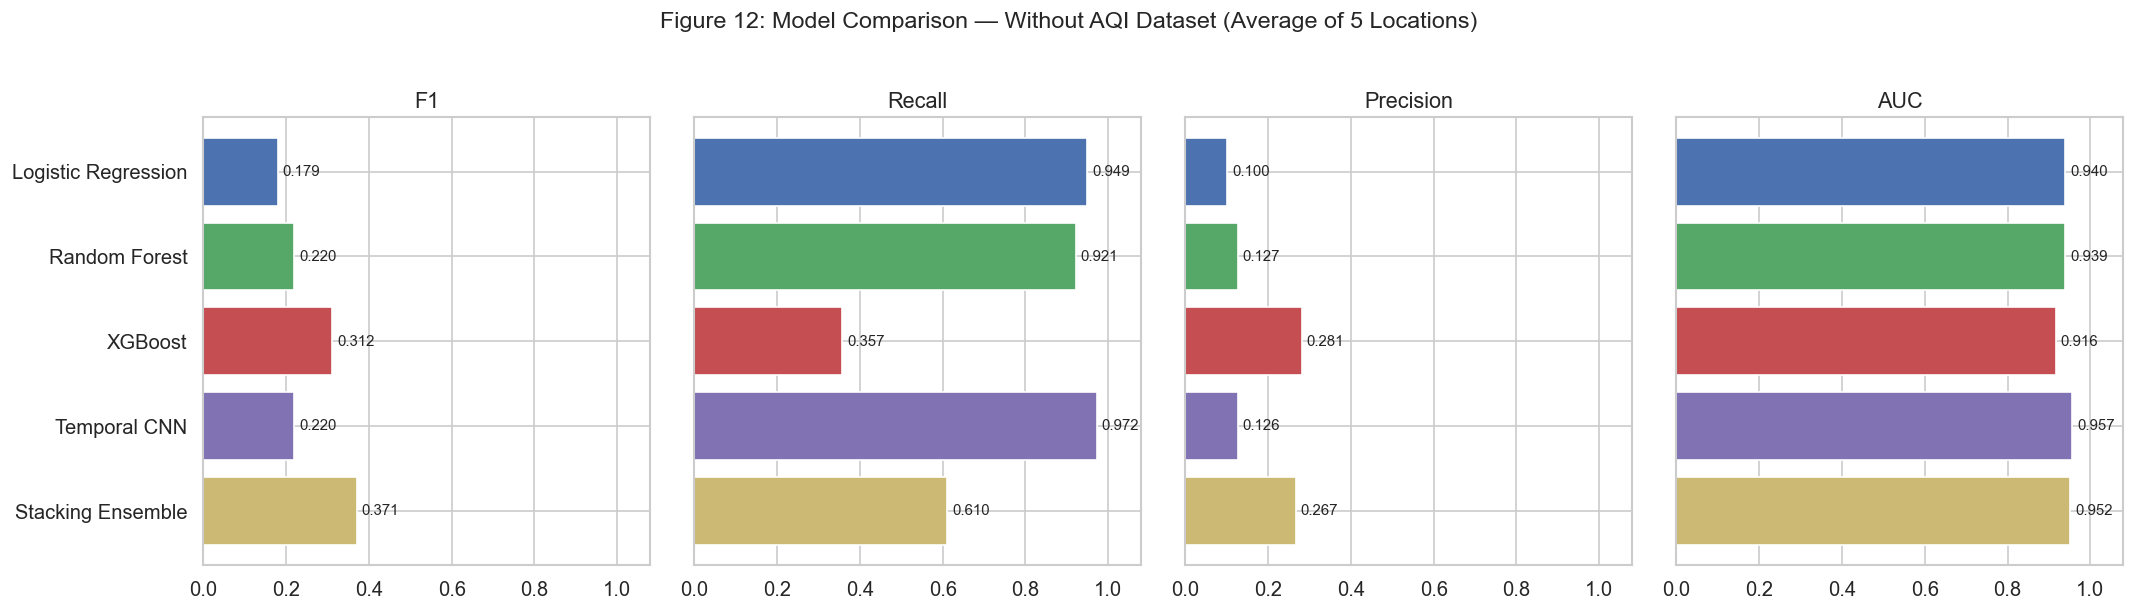
\includegraphics[keepaspectratio]{report_files/figure-pdf/cell-21-output-1.png}}

The following figure compares F1-scores for each model across the
datasets. Note how the \textbf{Without AQI} variant consistently
achieves the highest F1-scores for XGBoost and the Stacking Ensemble due
to its substantially larger training set, while the AQI-inclusive
variants show mixed results with performance degradation across most
models.

\pandocbounded{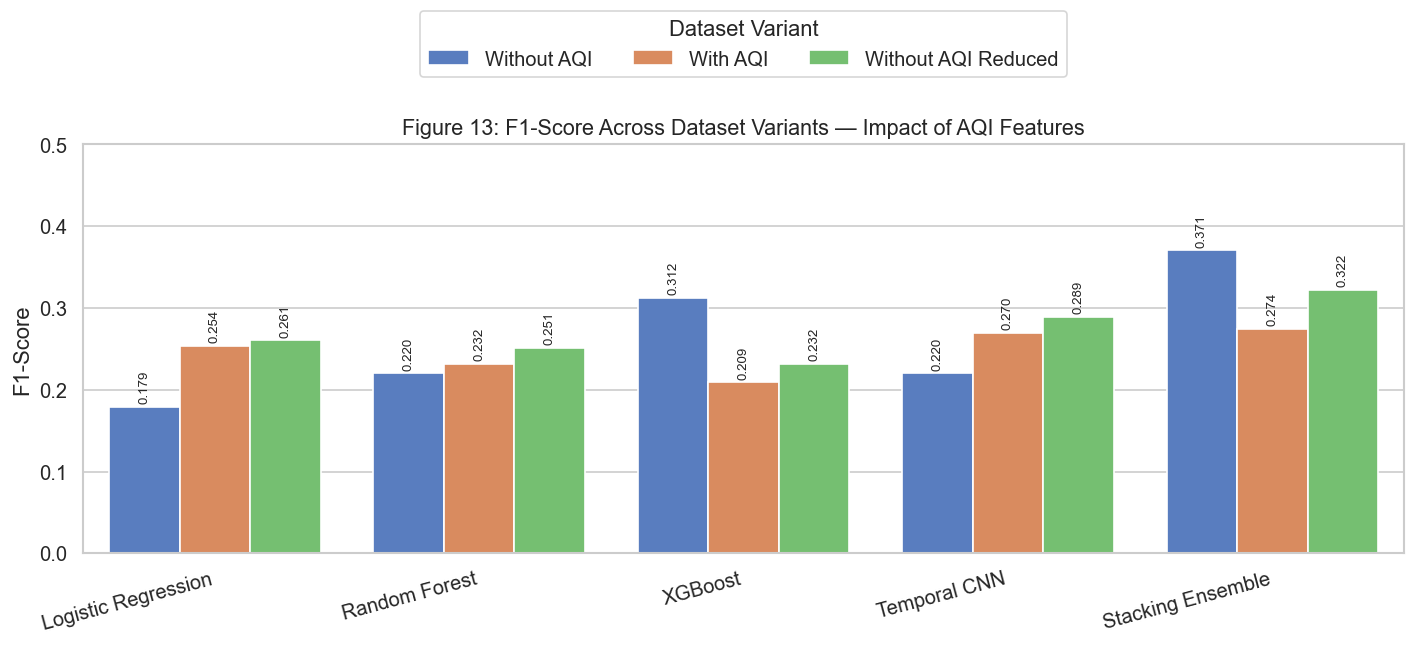
\includegraphics[keepaspectratio]{report_files/figure-pdf/cell-22-output-1.png}}

\section{Discussion \& Conclusion}\label{discussion-conclusion}

\textbf{1. The Stacking Ensemble achieves the highest F1-score (0.371).}
By combining predictions from all four base models in a sequential
pipeline, the ensemble balances recall (0.610) and precision (0.267)
more effectively than any individual model. This confirms that model
diversity and hierarchical feature augmentation provide complementary
predictive signal.

\textbf{2. The Temporal CNN achieves the highest recall (0.972) but the
lowest precision (0.126).} The CNN's ability to process 24-hour
sequences allows it to detect nearly all fog events, but it
over-predicts fog substantially.

\textbf{3. XGBoost provides the best precision-recall balance among
individual models (F1 = 0.312).} Its regularized gradient boosting and
F1-optimized threshold allow it to avoid many false positives while
maintaining moderate recall (0.357).

\textbf{4. AQI features provide no net benefit and lower performance.}
Across all five models, the \textbf{Without AQI} variant outperforms or
matches the \textbf{With AQI} variant. The controlled variant
outperforms the \textbf{With AQI} as well. This indicates that, at this
current time, the available volume of non-AQI based data provides a
clearer signal for predictive modeling approaches.

In conclusion, all modeling approaches faced the same significant
challenge: an inadequate positive class which resulted in a class
imbalance too dense to overcome. This challenge was further exacerbated
within the \textbf{With AQI} dataset variant, which was limited in size
by several order of magnitude compared to its historical, non-AQI
counterpart. Despite these limitations, this study demonstrates that
machine learning approaches can detect fog events with meaningful
recall, and that ensemble methods offer the best path forward for
balancing precision and recall. Future work should prioritize expanding
the dataset with additional fog observations, exploring advanced
resampling techniques such as SMOTE or focal loss to better address
class imbalance, and investigating real-time prediction systems that
incorporate satellite imagery and localized weather station data. With
California's Central Valley continuing to experience hazardous fog
conditions, the development of accurate predictive models remains
critical for improving public safety and reducing traffic-related
incidents.

\section{References}\label{references}

{[}1{]} E. Navarro, M. A. Lopez, and G. Ferris, ``Highway 99 in Tulare
County reopens after 59-vehicle pileup, CHP says,'' ABC30 Fresno
(KFSN-TV), Feb.~1, 2026. {[}Online{]}. Available:
https://abc30.com/post/150-vehicle-pileup-forces-total-closure-highway-99-tulare-county-officials-say/18516483/

{[}2{]} California Office of Traffic Safety, California FY2023 Annual
Report. Washington, DC, USA: National Highway Traffic Safety
Administration, May 2024. {[}Online{]}. Available:
https://www.nhtsa.gov/sites/nhtsa.gov/files/2024-05/CA\%20FY23\%20Annual\%20Report-tag.pdf

{[}3{]} L. Doermann, ``An unrelenting tule fog,'' NASA Earth
Observatory, National Aeronautics and Space Administration, Dec.~11,
2025. {[}Online{]}. Available:
https://science.nasa.gov/earth/earth-observatory/an-unrelenting-tule-fog/

{[}4{]} E. Gray, S. Gilardoni, D. Baldocchi, B. C. McDonald, M. C.
Facchini, and A. H. Goldstein, ``Impact of air pollution controls on
radiation fog frequency in the Central Valley of California,'' J.
Geophys. Res. Atmos., vol.~124, no. 10, pp.~5872--5895, Jun.~2019, doi:
10.1029/2018JD029419.

{[}5{]} K. Lakra and K. Avishek, ``A review on factors influencing fog
formation, classification, forecasting, detection and impacts,'' Rend.
Lincei Sci. Fis. Nat., vol.~33, no. 2, pp.~319--353, Mar.~2022, doi:
10.1007/s12210-022-01060-1.

{[}6{]} Open-Meteo, ``Free weather API,'' Open-Meteo.com. {[}Online{]}.
Available: https://open-meteo.com/. {[}Accessed: Mar.~16, 2026{]}.

{[}7{]} National Centers for Environmental Information, ``Data Access,''
NOAA NCEI. {[}Online{]}. Available:
https://www.ncei.noaa.gov/access/search/index. {[}Accessed: Mar.~16,
2026{]}.

{[}8{]} I. Gultepe et al., ``Fog research: A review of past achievements
and future perspectives,'' Pure Appl. Geophys., vol.~164,
pp.~1121--1159, Jun.~2007, doi: 10.1007/s00024-007-0211-x.

\section{Appendix A --- Pearson Coefficients for
Predictors}\label{appendix-a-pearson-coefficients-for-predictors}

\begin{longtable}[]{@{}llll@{}}
\toprule\noalign{}
& Weather Variable Correlations for Madera Airport & Pearson r &
\textbar r\textbar{} \\
\midrule\noalign{}
\endhead
\bottomrule\noalign{}
\endlastfoot
0 & soil\_temperature\_7\_to\_28cm & 0.377078 & 0.377078 \\
1 & surface\_pressure & -0.300592 & 0.300592 \\
2 & soil\_temperature\_0\_to\_7cm & 0.299374 & 0.299374 \\
3 & temperature\_2m & 0.256116 & 0.256116 \\
4 & relative\_humidity\_2m & -0.253132 & 0.253132 \\
5 & soil\_moisture\_0\_to\_7cm & -0.248368 & 0.248368 \\
6 & wind\_speed\_100m & 0.245728 & 0.245728 \\
7 & wind\_speed\_10m & 0.234854 & 0.234854 \\
8 & vapour\_pressure\_deficit & 0.220354 & 0.220354 \\
9 & wind\_gusts\_10m & 0.219550 & 0.219550 \\
10 & soil\_moisture\_7\_to\_28cm & -0.214151 & 0.214151 \\
11 & et0\_fao\_evapotranspiration & 0.135174 & 0.135174 \\
12 & dew\_point\_2m & 0.058017 & 0.058017 \\
13 & rain & -0.012212 & 0.012212 \\
14 & precipitation & -0.012071 & 0.012071 \\
\end{longtable}

\begin{longtable}[]{@{}llll@{}}
\toprule\noalign{}
& Weather Variable Correlations for Fresno Airport & Pearson r &
\textbar r\textbar{} \\
\midrule\noalign{}
\endhead
\bottomrule\noalign{}
\endlastfoot
0 & soil\_temperature\_7\_to\_28cm & 0.341873 & 0.341873 \\
1 & surface\_pressure & -0.288860 & 0.288860 \\
2 & soil\_temperature\_0\_to\_7cm & 0.281448 & 0.281448 \\
3 & temperature\_2m & 0.248664 & 0.248664 \\
4 & soil\_moisture\_0\_to\_7cm & -0.221295 & 0.221295 \\
5 & relative\_humidity\_2m & -0.215724 & 0.215724 \\
6 & wind\_gusts\_10m & 0.197985 & 0.197985 \\
7 & wind\_speed\_100m & 0.187792 & 0.187792 \\
8 & soil\_moisture\_7\_to\_28cm & -0.183458 & 0.183458 \\
9 & vapour\_pressure\_deficit & 0.182892 & 0.182892 \\
10 & wind\_speed\_10m & 0.178481 & 0.178481 \\
11 & dew\_point\_2m & 0.168501 & 0.168501 \\
12 & et0\_fao\_evapotranspiration & 0.149888 & 0.149888 \\
13 & precipitation & -0.016309 & 0.016309 \\
14 & rain & -0.016234 & 0.016234 \\
\end{longtable}

\begin{longtable}[]{@{}llll@{}}
\toprule\noalign{}
& Weather Variable Correlations for Visalia Airport & Pearson r &
\textbar r\textbar{} \\
\midrule\noalign{}
\endhead
\bottomrule\noalign{}
\endlastfoot
0 & soil\_temperature\_7\_to\_28cm & 0.372283 & 0.372283 \\
1 & surface\_pressure & -0.332688 & 0.332688 \\
2 & soil\_temperature\_0\_to\_7cm & 0.295677 & 0.295677 \\
3 & temperature\_2m & 0.243090 & 0.243090 \\
4 & relative\_humidity\_2m & -0.242687 & 0.242687 \\
5 & soil\_moisture\_0\_to\_7cm & -0.237460 & 0.237460 \\
6 & vapour\_pressure\_deficit & 0.222804 & 0.222804 \\
7 & soil\_moisture\_7\_to\_28cm & -0.220782 & 0.220782 \\
8 & wind\_speed\_10m & 0.200542 & 0.200542 \\
9 & wind\_speed\_100m & 0.198285 & 0.198285 \\
10 & wind\_gusts\_10m & 0.190970 & 0.190970 \\
11 & et0\_fao\_evapotranspiration & 0.116088 & 0.116088 \\
12 & dew\_point\_2m & 0.026175 & 0.026175 \\
13 & precipitation & 0.011267 & 0.011267 \\
14 & rain & 0.011156 & 0.011156 \\
\end{longtable}

\begin{longtable}[]{@{}llll@{}}
\toprule\noalign{}
& Weather Variable Correlations for Hanford Airport & Pearson r &
\textbar r\textbar{} \\
\midrule\noalign{}
\endhead
\bottomrule\noalign{}
\endlastfoot
0 & soil\_temperature\_7\_to\_28cm & 0.439807 & 0.439807 \\
1 & surface\_pressure & -0.356521 & 0.356521 \\
2 & soil\_temperature\_0\_to\_7cm & 0.324951 & 0.324951 \\
3 & wind\_speed\_100m & 0.279575 & 0.279575 \\
4 & wind\_speed\_10m & 0.261422 & 0.261422 \\
5 & temperature\_2m & 0.258619 & 0.258619 \\
6 & soil\_moisture\_0\_to\_7cm & -0.249494 & 0.249494 \\
7 & relative\_humidity\_2m & -0.231988 & 0.231988 \\
8 & vapour\_pressure\_deficit & 0.228645 & 0.228645 \\
9 & wind\_gusts\_10m & 0.226981 & 0.226981 \\
10 & soil\_moisture\_7\_to\_28cm & -0.223145 & 0.223145 \\
11 & et0\_fao\_evapotranspiration & 0.110157 & 0.110157 \\
12 & dew\_point\_2m & 0.067935 & 0.067935 \\
13 & precipitation & -0.005423 & 0.005423 \\
14 & rain & -0.005373 & 0.005373 \\
\end{longtable}

\begin{longtable}[]{@{}llll@{}}
\toprule\noalign{}
& Weather Variable Correlations for Bakersfield Airport & Pearson r &
\textbar r\textbar{} \\
\midrule\noalign{}
\endhead
\bottomrule\noalign{}
\endlastfoot
0 & soil\_temperature\_7\_to\_28cm & 0.183249 & 0.183249 \\
1 & surface\_pressure & -0.179847 & 0.179847 \\
2 & soil\_temperature\_0\_to\_7cm & 0.132013 & 0.132013 \\
3 & dew\_point\_2m & 0.120460 & 0.120460 \\
4 & temperature\_2m & 0.111254 & 0.111254 \\
5 & et0\_fao\_evapotranspiration & 0.083865 & 0.083865 \\
6 & relative\_humidity\_2m & -0.077174 & 0.077174 \\
7 & vapour\_pressure\_deficit & 0.060658 & 0.060658 \\
8 & soil\_moisture\_0\_to\_7cm & -0.056180 & 0.056180 \\
9 & soil\_moisture\_7\_to\_28cm & 0.037038 & 0.037038 \\
10 & wind\_speed\_100m & -0.033747 & 0.033747 \\
11 & wind\_speed\_10m & -0.033663 & 0.033663 \\
12 & wind\_gusts\_10m & 0.014346 & 0.014346 \\
13 & precipitation & 0.001574 & 0.001574 \\
14 & rain & 0.001512 & 0.001512 \\
\end{longtable}

\begin{longtable}[]{@{}llll@{}}
\toprule\noalign{}
& Weather Variable & Mean Pearson r & Mean \textbar r\textbar{} \\
\midrule\noalign{}
\endhead
\bottomrule\noalign{}
\endlastfoot
0 & soil\_temperature\_7\_to\_28cm & 0.342858 & 0.342858 \\
1 & surface\_pressure & -0.291702 & 0.291702 \\
2 & soil\_temperature\_0\_to\_7cm & 0.266693 & 0.266693 \\
3 & temperature\_2m & 0.223549 & 0.223549 \\
4 & relative\_humidity\_2m & -0.204141 & 0.204141 \\
5 & soil\_moisture\_0\_to\_7cm & -0.202559 & 0.202559 \\
6 & vapour\_pressure\_deficit & 0.183071 & 0.183071 \\
7 & wind\_speed\_100m & 0.175527 & 0.175527 \\
8 & wind\_gusts\_10m & 0.169967 & 0.169967 \\
9 & wind\_speed\_10m & 0.168327 & 0.168327 \\
10 & soil\_moisture\_7\_to\_28cm & -0.160900 & 0.160900 \\
11 & et0\_fao\_evapotranspiration & 0.119034 & 0.119034 \\
12 & dew\_point\_2m & 0.088217 & 0.088217 \\
13 & rain & -0.004230 & 0.004230 \\
14 & precipitation & -0.004193 & 0.004193 \\
\end{longtable}

\begin{longtable}[]{@{}llll@{}}
\toprule\noalign{}
& AQI Variable Correlations for Madera Airport & Pearson r &
\textbar r\textbar{} \\
\midrule\noalign{}
\endhead
\bottomrule\noalign{}
\endlastfoot
0 & pm2\_5 & -0.295918 & 0.295918 \\
1 & nitrogen\_dioxide & -0.162904 & 0.162904 \\
2 & pm10 & -0.125993 & 0.125993 \\
3 & dust & 0.087987 & 0.087987 \\
4 & aerosol\_optical\_depth & 0.022863 & 0.022863 \\
\end{longtable}

\begin{longtable}[]{@{}llll@{}}
\toprule\noalign{}
& AQI Variable Correlations for Fresno Airport & Pearson r &
\textbar r\textbar{} \\
\midrule\noalign{}
\endhead
\bottomrule\noalign{}
\endlastfoot
0 & pm2\_5 & -0.292328 & 0.292328 \\
1 & nitrogen\_dioxide & -0.199038 & 0.199038 \\
2 & pm10 & -0.163293 & 0.163293 \\
3 & dust & 0.089979 & 0.089979 \\
4 & aerosol\_optical\_depth & 0.020832 & 0.020832 \\
\end{longtable}

\begin{longtable}[]{@{}llll@{}}
\toprule\noalign{}
& AQI Variable Correlations for Visalia Airport & Pearson r &
\textbar r\textbar{} \\
\midrule\noalign{}
\endhead
\bottomrule\noalign{}
\endlastfoot
0 & dust & 0.104135 & 0.104135 \\
1 & nitrogen\_dioxide & -0.089018 & 0.089018 \\
2 & pm2\_5 & -0.061064 & 0.061064 \\
3 & aerosol\_optical\_depth & 0.036598 & 0.036598 \\
4 & pm10 & 0.022434 & 0.022434 \\
\end{longtable}

\begin{longtable}[]{@{}llll@{}}
\toprule\noalign{}
& AQI Variable Correlations for Hanford Airport & Pearson r &
\textbar r\textbar{} \\
\midrule\noalign{}
\endhead
\bottomrule\noalign{}
\endlastfoot
0 & pm2\_5 & -0.298534 & 0.298534 \\
1 & dust & 0.126767 & 0.126767 \\
2 & nitrogen\_dioxide & -0.067320 & 0.067320 \\
3 & pm10 & -0.032928 & 0.032928 \\
4 & aerosol\_optical\_depth & 0.021583 & 0.021583 \\
\end{longtable}

\begin{longtable}[]{@{}llll@{}}
\toprule\noalign{}
& AQI Variable Correlations for Bakersfield Airport & Pearson r &
\textbar r\textbar{} \\
\midrule\noalign{}
\endhead
\bottomrule\noalign{}
\endlastfoot
0 & dust & 0.212256 & 0.212256 \\
1 & pm10 & 0.189819 & 0.189819 \\
2 & nitrogen\_dioxide & -0.185887 & 0.185887 \\
3 & aerosol\_optical\_depth & 0.148394 & 0.148394 \\
4 & pm2\_5 & 0.069993 & 0.069993 \\
\end{longtable}

\begin{longtable}[]{@{}llll@{}}
\toprule\noalign{}
& AQI Variable & Mean Pearson r & Mean \textbar r\textbar{} \\
\midrule\noalign{}
\endhead
\bottomrule\noalign{}
\endlastfoot
0 & pm2\_5 & -0.175570 & 0.175570 \\
1 & nitrogen\_dioxide & -0.140834 & 0.140834 \\
2 & dust & 0.124225 & 0.124225 \\
3 & aerosol\_optical\_depth & 0.050054 & 0.050054 \\
4 & pm10 & -0.021992 & 0.021992 \\
\end{longtable}

\begin{longtable}[]{@{}llll@{}}
\toprule\noalign{}
& Inferred Variable Correlations for Madera Airport & Pearson r &
\textbar r\textbar{} \\
\midrule\noalign{}
\endhead
\bottomrule\noalign{}
\endlastfoot
0 & previous\_night\_low & 0.360346 & 0.360346 \\
1 & dewpoint\_depression & 0.237296 & 0.237296 \\
2 & cooling\_rate\_6h & -0.109337 & 0.109337 \\
3 & cooling\_rate\_12h & -0.106983 & 0.106983 \\
\end{longtable}

\begin{longtable}[]{@{}llll@{}}
\toprule\noalign{}
& Inferred Variable Correlations for Fresno Airport & Pearson r &
\textbar r\textbar{} \\
\midrule\noalign{}
\endhead
\bottomrule\noalign{}
\endlastfoot
0 & previous\_night\_low & 0.328798 & 0.328798 \\
1 & dewpoint\_depression & 0.188694 & 0.188694 \\
2 & cooling\_rate\_12h & -0.085631 & 0.085631 \\
3 & cooling\_rate\_6h & -0.051198 & 0.051198 \\
\end{longtable}

\begin{longtable}[]{@{}llll@{}}
\toprule\noalign{}
& Inferred Variable Correlations for Visalia Airport & Pearson r &
\textbar r\textbar{} \\
\midrule\noalign{}
\endhead
\bottomrule\noalign{}
\endlastfoot
0 & previous\_night\_low & 0.352691 & 0.352691 \\
1 & dewpoint\_depression & 0.235897 & 0.235897 \\
2 & cooling\_rate\_12h & -0.140694 & 0.140694 \\
3 & cooling\_rate\_6h & -0.135416 & 0.135416 \\
\end{longtable}

\begin{longtable}[]{@{}llll@{}}
\toprule\noalign{}
& Inferred Variable Correlations for Hanford Airport & Pearson r &
\textbar r\textbar{} \\
\midrule\noalign{}
\endhead
\bottomrule\noalign{}
\endlastfoot
0 & previous\_night\_low & 0.417615 & 0.417615 \\
1 & dewpoint\_depression & 0.227464 & 0.227464 \\
2 & cooling\_rate\_12h & -0.193214 & 0.193214 \\
3 & cooling\_rate\_6h & -0.187136 & 0.187136 \\
\end{longtable}

\begin{longtable}[]{@{}llll@{}}
\toprule\noalign{}
& Inferred Variable Correlations for Bakersfield Airport & Pearson r &
\textbar r\textbar{} \\
\midrule\noalign{}
\endhead
\bottomrule\noalign{}
\endlastfoot
0 & previous\_night\_low & 0.184777 & 0.184777 \\
1 & cooling\_rate\_12h & -0.079690 & 0.079690 \\
2 & dewpoint\_depression & 0.050397 & 0.050397 \\
3 & cooling\_rate\_6h & -0.001806 & 0.001806 \\
\end{longtable}

\begin{longtable}[]{@{}llll@{}}
\toprule\noalign{}
& Inferred Variable & Mean Pearson r & Mean \textbar r\textbar{} \\
\midrule\noalign{}
\endhead
\bottomrule\noalign{}
\endlastfoot
0 & previous\_night\_low & 0.328846 & 0.328846 \\
1 & dewpoint\_depression & 0.187950 & 0.187950 \\
2 & cooling\_rate\_12h & -0.121242 & 0.121242 \\
3 & cooling\_rate\_6h & -0.096979 & 0.096979 \\
\end{longtable}

\section{Appendix B --- K-Means Clustering Raw
Results}\label{appendix-b-k-means-clustering-raw-results}

\begin{Shaded}
\begin{Highlighting}[]
\NormalTok{LOCATION }\DecValTok{10}
\OperatorTok{{-}{-}{-}{-}{-}{-}{-}{-}{-}{-}{-}{-}{-}{-}{-}{-}{-}{-}{-}{-}{-}{-}{-}{-}{-}{-}{-}{-}{-}{-}{-}{-}{-}{-}{-}{-}{-}{-}{-}{-}{-}{-}{-}{-}{-}{-}{-}{-}{-}{-}{-}{-}{-}{-}{-}{-}{-}{-}{-}{-}{-}{-}{-}{-}{-}{-}{-}{-}{-}{-}{-}{-}{-}{-}{-}{-}{-}{-}{-}{-}}
\NormalTok{WITHOUT AQI (}\BuiltInTok{all}\NormalTok{ rows, no AQI features):}
\NormalTok{  Records: }\DecValTok{365120}
\NormalTok{  Inertia: }\FloatTok{2617205.83}
\NormalTok{  Silhouette Score: }\FloatTok{0.2016}
\NormalTok{  Davies}\OperatorTok{{-}}\NormalTok{Bouldin Index: }\FloatTok{1.4035}

\NormalTok{  Feature Variance Across Clusters (}\BuiltInTok{sorted}\NormalTok{, }\DecValTok{19}\NormalTok{ features):}
\NormalTok{    rain: }\FloatTok{26.34}\OperatorTok{\%}
\NormalTok{    precipitation: }\FloatTok{26.16}\OperatorTok{\%}
\NormalTok{    vapour\_pressure\_deficit: }\FloatTok{4.23}\OperatorTok{\%}
\NormalTok{    dewpoint\_depression: }\FloatTok{3.95}\OperatorTok{\%}
\NormalTok{    wind\_speed\_100m: }\FloatTok{3.88}\OperatorTok{\%}
\NormalTok{    relative\_humidity\_2m: }\FloatTok{3.51}\OperatorTok{\%}
\NormalTok{    soil\_temperature\_0\_to\_7cm: }\FloatTok{3.38}\OperatorTok{\%}
\NormalTok{    wind\_speed\_10m: }\FloatTok{3.38}\OperatorTok{\%}
\NormalTok{    temperature\_2m: }\FloatTok{3.29}\OperatorTok{\%}
\NormalTok{    wind\_gusts\_10m: }\FloatTok{3.23}\OperatorTok{\%}
\NormalTok{    soil\_moisture\_0\_to\_7cm: }\FloatTok{3.09}\OperatorTok{\%}
\NormalTok{    et0\_fao\_evapotranspiration: }\FloatTok{2.79}\OperatorTok{\%}
\NormalTok{    soil\_temperature\_7\_to\_28cm: }\FloatTok{2.75}\OperatorTok{\%}
\NormalTok{    previous\_night\_low: }\FloatTok{2.28}\OperatorTok{\%}
\NormalTok{    soil\_moisture\_7\_to\_28cm: }\FloatTok{1.91}\OperatorTok{\%}
\NormalTok{    cooling\_rate\_6h: }\FloatTok{1.83}\OperatorTok{\%}
\NormalTok{    cooling\_rate\_12h: }\FloatTok{1.79}\OperatorTok{\%}
\NormalTok{    surface\_pressure: }\FloatTok{1.39}\OperatorTok{\%}
\NormalTok{    dew\_point\_2m: }\FloatTok{0.82}\OperatorTok{\%}

\NormalTok{WITH AQI (filtered rows, }\ControlFlowTok{with}\NormalTok{ AQI features):}
\NormalTok{  Records: }\DecValTok{25691}
\NormalTok{  Inertia: }\FloatTok{268380.45}
\NormalTok{  Silhouette Score: }\FloatTok{0.1826}
\NormalTok{  Davies}\OperatorTok{{-}}\NormalTok{Bouldin Index: }\FloatTok{1.5409}

\NormalTok{  Feature Variance Across Clusters (}\BuiltInTok{sorted}\NormalTok{, }\DecValTok{24}\NormalTok{ features):}
\NormalTok{    rain: }\FloatTok{27.58}\OperatorTok{\%}
\NormalTok{    precipitation: }\FloatTok{26.96}\OperatorTok{\%}
\NormalTok{    pm10: }\FloatTok{4.32}\OperatorTok{\%}
\NormalTok{    dust: }\FloatTok{3.85}\OperatorTok{\%}
\NormalTok{    soil\_moisture\_0\_to\_7cm: }\FloatTok{2.84}\OperatorTok{\%}
\NormalTok{    relative\_humidity\_2m: }\FloatTok{2.50}\OperatorTok{\%}
\NormalTok{    wind\_speed\_10m: }\FloatTok{2.29}\OperatorTok{\%}
\NormalTok{    soil\_temperature\_7\_to\_28cm: }\FloatTok{2.29}\OperatorTok{\%}
\NormalTok{    wind\_speed\_100m: }\FloatTok{2.29}\OperatorTok{\%}
\NormalTok{    wind\_gusts\_10m: }\FloatTok{2.29}\OperatorTok{\%}
\NormalTok{    pm2\_5: }\FloatTok{2.27}\OperatorTok{\%}
\NormalTok{    soil\_temperature\_0\_to\_7cm: }\FloatTok{2.23}\OperatorTok{\%}
\NormalTok{    dewpoint\_depression: }\FloatTok{2.21}\OperatorTok{\%}
\NormalTok{    temperature\_2m: }\FloatTok{2.20}\OperatorTok{\%}
\NormalTok{    previous\_night\_low: }\FloatTok{2.11}\OperatorTok{\%}
\NormalTok{    vapour\_pressure\_deficit: }\FloatTok{2.05}\OperatorTok{\%}
\NormalTok{    et0\_fao\_evapotranspiration: }\FloatTok{1.80}\OperatorTok{\%}
\NormalTok{    cooling\_rate\_6h: }\FloatTok{1.59}\OperatorTok{\%}
\NormalTok{    soil\_moisture\_7\_to\_28cm: }\FloatTok{1.46}\OperatorTok{\%}
\NormalTok{    surface\_pressure: }\FloatTok{1.38}\OperatorTok{\%}
\NormalTok{    cooling\_rate\_12h: }\FloatTok{1.29}\OperatorTok{\%}
\NormalTok{    nitrogen\_dioxide: }\FloatTok{0.94}\OperatorTok{\%}
\NormalTok{    aerosol\_optical\_depth: }\FloatTok{0.77}\OperatorTok{\%}
\NormalTok{    dew\_point\_2m: }\FloatTok{0.48}\OperatorTok{\%}

\NormalTok{WITHOUT AQI REDUCED (filtered rows, no AQI features):}
\NormalTok{  Records: }\DecValTok{25691}
\NormalTok{  Inertia: }\FloatTok{166323.66}
\NormalTok{  Silhouette Score: }\FloatTok{0.2233}
\NormalTok{  Davies}\OperatorTok{{-}}\NormalTok{Bouldin Index: }\FloatTok{1.3952}

\NormalTok{  Feature Variance Across Clusters (}\BuiltInTok{sorted}\NormalTok{, }\DecValTok{19}\NormalTok{ features):}
\NormalTok{    rain: }\FloatTok{30.67}\OperatorTok{\%}
\NormalTok{    precipitation: }\FloatTok{30.07}\OperatorTok{\%}
\NormalTok{    soil\_moisture\_0\_to\_7cm: }\FloatTok{2.93}\OperatorTok{\%}
\NormalTok{    relative\_humidity\_2m: }\FloatTok{2.87}\OperatorTok{\%}
\NormalTok{    wind\_speed\_100m: }\FloatTok{2.86}\OperatorTok{\%}
\NormalTok{    dewpoint\_depression: }\FloatTok{2.84}\OperatorTok{\%}
\NormalTok{    soil\_temperature\_0\_to\_7cm: }\FloatTok{2.81}\OperatorTok{\%}
\NormalTok{    vapour\_pressure\_deficit: }\FloatTok{2.75}\OperatorTok{\%}
\NormalTok{    wind\_speed\_10m: }\FloatTok{2.75}\OperatorTok{\%}
\NormalTok{    temperature\_2m: }\FloatTok{2.71}\OperatorTok{\%}
\NormalTok{    wind\_gusts\_10m: }\FloatTok{2.54}\OperatorTok{\%}
\NormalTok{    soil\_temperature\_7\_to\_28cm: }\FloatTok{2.43}\OperatorTok{\%}
\NormalTok{    et0\_fao\_evapotranspiration: }\FloatTok{2.41}\OperatorTok{\%}
\NormalTok{    previous\_night\_low: }\FloatTok{2.17}\OperatorTok{\%}
\NormalTok{    cooling\_rate\_6h: }\FloatTok{1.89}\OperatorTok{\%}
\NormalTok{    soil\_moisture\_7\_to\_28cm: }\FloatTok{1.62}\OperatorTok{\%}
\NormalTok{    cooling\_rate\_12h: }\FloatTok{1.61}\OperatorTok{\%}
\NormalTok{    surface\_pressure: }\FloatTok{1.50}\OperatorTok{\%}
\NormalTok{    dew\_point\_2m: }\FloatTok{0.57}\OperatorTok{\%}

\OperatorTok{================================================================================}

\NormalTok{LOCATION }\DecValTok{6}
\OperatorTok{{-}{-}{-}{-}{-}{-}{-}{-}{-}{-}{-}{-}{-}{-}{-}{-}{-}{-}{-}{-}{-}{-}{-}{-}{-}{-}{-}{-}{-}{-}{-}{-}{-}{-}{-}{-}{-}{-}{-}{-}{-}{-}{-}{-}{-}{-}{-}{-}{-}{-}{-}{-}{-}{-}{-}{-}{-}{-}{-}{-}{-}{-}{-}{-}{-}{-}{-}{-}{-}{-}{-}{-}{-}{-}{-}{-}{-}{-}{-}{-}}
\NormalTok{WITHOUT AQI (}\BuiltInTok{all}\NormalTok{ rows, no AQI features):}
\NormalTok{  Records: }\DecValTok{164421}
\NormalTok{  Inertia: }\FloatTok{1063459.57}
\NormalTok{  Silhouette Score: }\FloatTok{0.2088}
\NormalTok{  Davies}\OperatorTok{{-}}\NormalTok{Bouldin Index: }\FloatTok{1.3889}

\NormalTok{  Feature Variance Across Clusters (}\BuiltInTok{sorted}\NormalTok{, }\DecValTok{19}\NormalTok{ features):}
\NormalTok{    rain: }\FloatTok{25.95}\OperatorTok{\%}
\NormalTok{    precipitation: }\FloatTok{25.94}\OperatorTok{\%}
\NormalTok{    soil\_moisture\_0\_to\_7cm: }\FloatTok{4.35}\OperatorTok{\%}
\NormalTok{    relative\_humidity\_2m: }\FloatTok{3.49}\OperatorTok{\%}
\NormalTok{    soil\_temperature\_0\_to\_7cm: }\FloatTok{3.31}\OperatorTok{\%}
\NormalTok{    soil\_temperature\_7\_to\_28cm: }\FloatTok{3.30}\OperatorTok{\%}
\NormalTok{    dewpoint\_depression: }\FloatTok{3.26}\OperatorTok{\%}
\NormalTok{    soil\_moisture\_7\_to\_28cm: }\FloatTok{3.24}\OperatorTok{\%}
\NormalTok{    temperature\_2m: }\FloatTok{3.15}\OperatorTok{\%}
\NormalTok{    vapour\_pressure\_deficit: }\FloatTok{3.11}\OperatorTok{\%}
\NormalTok{    wind\_speed\_100m: }\FloatTok{3.02}\OperatorTok{\%}
\NormalTok{    et0\_fao\_evapotranspiration: }\FloatTok{2.80}\OperatorTok{\%}
\NormalTok{    wind\_speed\_10m: }\FloatTok{2.75}\OperatorTok{\%}
\NormalTok{    wind\_gusts\_10m: }\FloatTok{2.73}\OperatorTok{\%}
\NormalTok{    previous\_night\_low: }\FloatTok{2.65}\OperatorTok{\%}
\NormalTok{    cooling\_rate\_6h: }\FloatTok{2.32}\OperatorTok{\%}
\NormalTok{    cooling\_rate\_12h: }\FloatTok{2.07}\OperatorTok{\%}
\NormalTok{    surface\_pressure: }\FloatTok{1.84}\OperatorTok{\%}
\NormalTok{    dew\_point\_2m: }\FloatTok{0.73}\OperatorTok{\%}

\NormalTok{WITH AQI (filtered rows, }\ControlFlowTok{with}\NormalTok{ AQI features):}
\NormalTok{  Records: }\DecValTok{25558}
\NormalTok{  Inertia: }\FloatTok{262365.04}
\NormalTok{  Silhouette Score: }\FloatTok{0.2087}
\NormalTok{  Davies}\OperatorTok{{-}}\NormalTok{Bouldin Index: }\FloatTok{1.4584}

\NormalTok{  Feature Variance Across Clusters (}\BuiltInTok{sorted}\NormalTok{, }\DecValTok{24}\NormalTok{ features):}
\NormalTok{    rain: }\FloatTok{23.10}\OperatorTok{\%}
\NormalTok{    precipitation: }\FloatTok{23.01}\OperatorTok{\%}
\NormalTok{    dust: }\FloatTok{7.94}\OperatorTok{\%}
\NormalTok{    pm10: }\FloatTok{4.48}\OperatorTok{\%}
\NormalTok{    soil\_moisture\_0\_to\_7cm: }\FloatTok{3.41}\OperatorTok{\%}
\NormalTok{    relative\_humidity\_2m: }\FloatTok{2.63}\OperatorTok{\%}
\NormalTok{    wind\_gusts\_10m: }\FloatTok{2.62}\OperatorTok{\%}
\NormalTok{    wind\_speed\_100m: }\FloatTok{2.61}\OperatorTok{\%}
\NormalTok{    wind\_speed\_10m: }\FloatTok{2.57}\OperatorTok{\%}
\NormalTok{    soil\_temperature\_0\_to\_7cm: }\FloatTok{2.54}\OperatorTok{\%}
\NormalTok{    temperature\_2m: }\FloatTok{2.47}\OperatorTok{\%}
\NormalTok{    dewpoint\_depression: }\FloatTok{2.43}\OperatorTok{\%}
\NormalTok{    soil\_temperature\_7\_to\_28cm: }\FloatTok{2.42}\OperatorTok{\%}
\NormalTok{    vapour\_pressure\_deficit: }\FloatTok{2.31}\OperatorTok{\%}
\NormalTok{    et0\_fao\_evapotranspiration: }\FloatTok{2.21}\OperatorTok{\%}
\NormalTok{    soil\_moisture\_7\_to\_28cm: }\FloatTok{2.05}\OperatorTok{\%}
\NormalTok{    previous\_night\_low: }\FloatTok{2.04}\OperatorTok{\%}
\NormalTok{    nitrogen\_dioxide: }\FloatTok{2.00}\OperatorTok{\%}
\NormalTok{    cooling\_rate\_6h: }\FloatTok{1.76}\OperatorTok{\%}
\NormalTok{    cooling\_rate\_12h: }\FloatTok{1.56}\OperatorTok{\%}
\NormalTok{    surface\_pressure: }\FloatTok{1.56}\OperatorTok{\%}
\NormalTok{    pm2\_5: }\FloatTok{1.14}\OperatorTok{\%}
\NormalTok{    dew\_point\_2m: }\FloatTok{0.68}\OperatorTok{\%}
\NormalTok{    aerosol\_optical\_depth: }\FloatTok{0.46}\OperatorTok{\%}

\NormalTok{WITHOUT AQI REDUCED (filtered rows, no AQI features):}
\NormalTok{  Records: }\DecValTok{25558}
\NormalTok{  Inertia: }\FloatTok{164047.65}
\NormalTok{  Silhouette Score: }\FloatTok{0.2087}
\NormalTok{  Davies}\OperatorTok{{-}}\NormalTok{Bouldin Index: }\FloatTok{1.3686}

\NormalTok{  Feature Variance Across Clusters (}\BuiltInTok{sorted}\NormalTok{, }\DecValTok{19}\NormalTok{ features):}
\NormalTok{    rain: }\FloatTok{26.36}\OperatorTok{\%}
\NormalTok{    precipitation: }\FloatTok{26.27}\OperatorTok{\%}
\NormalTok{    soil\_moisture\_0\_to\_7cm: }\FloatTok{4.18}\OperatorTok{\%}
\NormalTok{    relative\_humidity\_2m: }\FloatTok{3.38}\OperatorTok{\%}
\NormalTok{    soil\_temperature\_7\_to\_28cm: }\FloatTok{3.31}\OperatorTok{\%}
\NormalTok{    soil\_temperature\_0\_to\_7cm: }\FloatTok{3.30}\OperatorTok{\%}
\NormalTok{    soil\_moisture\_7\_to\_28cm: }\FloatTok{3.28}\OperatorTok{\%}
\NormalTok{    dewpoint\_depression: }\FloatTok{3.20}\OperatorTok{\%}
\NormalTok{    temperature\_2m: }\FloatTok{3.13}\OperatorTok{\%}
\NormalTok{    vapour\_pressure\_deficit: }\FloatTok{2.99}\OperatorTok{\%}
\NormalTok{    et0\_fao\_evapotranspiration: }\FloatTok{2.83}\OperatorTok{\%}
\NormalTok{    wind\_speed\_100m: }\FloatTok{2.78}\OperatorTok{\%}
\NormalTok{    previous\_night\_low: }\FloatTok{2.70}\OperatorTok{\%}
\NormalTok{    wind\_gusts\_10m: }\FloatTok{2.67}\OperatorTok{\%}
\NormalTok{    wind\_speed\_10m: }\FloatTok{2.63}\OperatorTok{\%}
\NormalTok{    cooling\_rate\_6h: }\FloatTok{2.36}\OperatorTok{\%}
\NormalTok{    cooling\_rate\_12h: }\FloatTok{1.93}\OperatorTok{\%}
\NormalTok{    surface\_pressure: }\FloatTok{1.83}\OperatorTok{\%}
\NormalTok{    dew\_point\_2m: }\FloatTok{0.87}\OperatorTok{\%}

\OperatorTok{================================================================================}

\NormalTok{LOCATION }\DecValTok{7}
\OperatorTok{{-}{-}{-}{-}{-}{-}{-}{-}{-}{-}{-}{-}{-}{-}{-}{-}{-}{-}{-}{-}{-}{-}{-}{-}{-}{-}{-}{-}{-}{-}{-}{-}{-}{-}{-}{-}{-}{-}{-}{-}{-}{-}{-}{-}{-}{-}{-}{-}{-}{-}{-}{-}{-}{-}{-}{-}{-}{-}{-}{-}{-}{-}{-}{-}{-}{-}{-}{-}{-}{-}{-}{-}{-}{-}{-}{-}{-}{-}{-}{-}}
\NormalTok{WITHOUT AQI (}\BuiltInTok{all}\NormalTok{ rows, no AQI features):}
\NormalTok{  Records: }\DecValTok{392427}
\NormalTok{  Inertia: }\FloatTok{2526989.85}
\NormalTok{  Silhouette Score: }\FloatTok{0.2119}
\NormalTok{  Davies}\OperatorTok{{-}}\NormalTok{Bouldin Index: }\FloatTok{1.3617}

\NormalTok{  Feature Variance Across Clusters (}\BuiltInTok{sorted}\NormalTok{, }\DecValTok{19}\NormalTok{ features):}
\NormalTok{    precipitation: }\FloatTok{23.50}\OperatorTok{\%}
\NormalTok{    rain: }\FloatTok{23.49}\OperatorTok{\%}
\NormalTok{    soil\_moisture\_0\_to\_7cm: }\FloatTok{4.72}\OperatorTok{\%}
\NormalTok{    relative\_humidity\_2m: }\FloatTok{3.88}\OperatorTok{\%}
\NormalTok{    soil\_temperature\_7\_to\_28cm: }\FloatTok{3.64}\OperatorTok{\%}
\NormalTok{    soil\_temperature\_0\_to\_7cm: }\FloatTok{3.56}\OperatorTok{\%}
\NormalTok{    soil\_moisture\_7\_to\_28cm: }\FloatTok{3.56}\OperatorTok{\%}
\NormalTok{    dewpoint\_depression: }\FloatTok{3.51}\OperatorTok{\%}
\NormalTok{    wind\_speed\_100m: }\FloatTok{3.44}\OperatorTok{\%}
\NormalTok{    temperature\_2m: }\FloatTok{3.40}\OperatorTok{\%}
\NormalTok{    vapour\_pressure\_deficit: }\FloatTok{3.32}\OperatorTok{\%}
\NormalTok{    wind\_gusts\_10m: }\FloatTok{3.12}\OperatorTok{\%}
\NormalTok{    wind\_speed\_10m: }\FloatTok{3.08}\OperatorTok{\%}
\NormalTok{    et0\_fao\_evapotranspiration: }\FloatTok{3.02}\OperatorTok{\%}
\NormalTok{    previous\_night\_low: }\FloatTok{2.93}\OperatorTok{\%}
\NormalTok{    cooling\_rate\_6h: }\FloatTok{2.62}\OperatorTok{\%}
\NormalTok{    cooling\_rate\_12h: }\FloatTok{2.28}\OperatorTok{\%}
\NormalTok{    surface\_pressure: }\FloatTok{1.89}\OperatorTok{\%}
\NormalTok{    dew\_point\_2m: }\FloatTok{1.04}\OperatorTok{\%}

\NormalTok{WITH AQI (filtered rows, }\ControlFlowTok{with}\NormalTok{ AQI features):}
\NormalTok{  Records: }\DecValTok{25748}
\NormalTok{  Inertia: }\FloatTok{259556.46}
\NormalTok{  Silhouette Score: }\FloatTok{0.1905}
\NormalTok{  Davies}\OperatorTok{{-}}\NormalTok{Bouldin Index: }\FloatTok{1.4757}

\NormalTok{  Feature Variance Across Clusters (}\BuiltInTok{sorted}\NormalTok{, }\DecValTok{24}\NormalTok{ features):}
\NormalTok{    precipitation: }\FloatTok{25.13}\OperatorTok{\%}
\NormalTok{    rain: }\FloatTok{25.09}\OperatorTok{\%}
\NormalTok{    dust: }\FloatTok{5.79}\OperatorTok{\%}
\NormalTok{    soil\_moisture\_0\_to\_7cm: }\FloatTok{3.67}\OperatorTok{\%}
\NormalTok{    soil\_temperature\_7\_to\_28cm: }\FloatTok{2.84}\OperatorTok{\%}
\NormalTok{    pm10: }\FloatTok{2.83}\OperatorTok{\%}
\NormalTok{    relative\_humidity\_2m: }\FloatTok{2.70}\OperatorTok{\%}
\NormalTok{    soil\_temperature\_0\_to\_7cm: }\FloatTok{2.63}\OperatorTok{\%}
\NormalTok{    dewpoint\_depression: }\FloatTok{2.44}\OperatorTok{\%}
\NormalTok{    temperature\_2m: }\FloatTok{2.43}\OperatorTok{\%}
\NormalTok{    soil\_moisture\_7\_to\_28cm: }\FloatTok{2.39}\OperatorTok{\%}
\NormalTok{    wind\_speed\_100m: }\FloatTok{2.32}\OperatorTok{\%}
\NormalTok{    previous\_night\_low: }\FloatTok{2.30}\OperatorTok{\%}
\NormalTok{    vapour\_pressure\_deficit: }\FloatTok{2.28}\OperatorTok{\%}
\NormalTok{    et0\_fao\_evapotranspiration: }\FloatTok{2.24}\OperatorTok{\%}
\NormalTok{    cooling\_rate\_6h: }\FloatTok{2.10}\OperatorTok{\%}
\NormalTok{    wind\_gusts\_10m: }\FloatTok{1.94}\OperatorTok{\%}
\NormalTok{    wind\_speed\_10m: }\FloatTok{1.93}\OperatorTok{\%}
\NormalTok{    cooling\_rate\_12h: }\FloatTok{1.67}\OperatorTok{\%}
\NormalTok{    surface\_pressure: }\FloatTok{1.52}\OperatorTok{\%}
\NormalTok{    nitrogen\_dioxide: }\FloatTok{1.36}\OperatorTok{\%}
\NormalTok{    pm2\_5: }\FloatTok{0.88}\OperatorTok{\%}
\NormalTok{    dew\_point\_2m: }\FloatTok{0.77}\OperatorTok{\%}
\NormalTok{    aerosol\_optical\_depth: }\FloatTok{0.75}\OperatorTok{\%}

\NormalTok{WITHOUT AQI REDUCED (filtered rows, no AQI features):}
\NormalTok{  Records: }\DecValTok{25748}
\NormalTok{  Inertia: }\FloatTok{159702.68}
\NormalTok{  Silhouette Score: }\FloatTok{0.2038}
\NormalTok{  Davies}\OperatorTok{{-}}\NormalTok{Bouldin Index: }\FloatTok{1.3619}

\NormalTok{  Feature Variance Across Clusters (}\BuiltInTok{sorted}\NormalTok{, }\DecValTok{19}\NormalTok{ features):}
\NormalTok{    precipitation: }\FloatTok{27.12}\OperatorTok{\%}
\NormalTok{    rain: }\FloatTok{27.09}\OperatorTok{\%}
\NormalTok{    soil\_moisture\_0\_to\_7cm: }\FloatTok{3.98}\OperatorTok{\%}
\NormalTok{    relative\_humidity\_2m: }\FloatTok{3.21}\OperatorTok{\%}
\NormalTok{    soil\_temperature\_7\_to\_28cm: }\FloatTok{3.14}\OperatorTok{\%}
\NormalTok{    soil\_temperature\_0\_to\_7cm: }\FloatTok{3.11}\OperatorTok{\%}
\NormalTok{    wind\_speed\_100m: }\FloatTok{3.04}\OperatorTok{\%}
\NormalTok{    temperature\_2m: }\FloatTok{2.97}\OperatorTok{\%}
\NormalTok{    dewpoint\_depression: }\FloatTok{2.97}\OperatorTok{\%}
\NormalTok{    soil\_moisture\_7\_to\_28cm: }\FloatTok{2.88}\OperatorTok{\%}
\NormalTok{    vapour\_pressure\_deficit: }\FloatTok{2.78}\OperatorTok{\%}
\NormalTok{    wind\_speed\_10m: }\FloatTok{2.72}\OperatorTok{\%}
\NormalTok{    et0\_fao\_evapotranspiration: }\FloatTok{2.71}\OperatorTok{\%}
\NormalTok{    wind\_gusts\_10m: }\FloatTok{2.69}\OperatorTok{\%}
\NormalTok{    previous\_night\_low: }\FloatTok{2.62}\OperatorTok{\%}
\NormalTok{    cooling\_rate\_6h: }\FloatTok{2.35}\OperatorTok{\%}
\NormalTok{    cooling\_rate\_12h: }\FloatTok{1.91}\OperatorTok{\%}
\NormalTok{    surface\_pressure: }\FloatTok{1.75}\OperatorTok{\%}
\NormalTok{    dew\_point\_2m: }\FloatTok{0.95}\OperatorTok{\%}

\OperatorTok{================================================================================}

\NormalTok{LOCATION }\DecValTok{8}
\OperatorTok{{-}{-}{-}{-}{-}{-}{-}{-}{-}{-}{-}{-}{-}{-}{-}{-}{-}{-}{-}{-}{-}{-}{-}{-}{-}{-}{-}{-}{-}{-}{-}{-}{-}{-}{-}{-}{-}{-}{-}{-}{-}{-}{-}{-}{-}{-}{-}{-}{-}{-}{-}{-}{-}{-}{-}{-}{-}{-}{-}{-}{-}{-}{-}{-}{-}{-}{-}{-}{-}{-}{-}{-}{-}{-}{-}{-}{-}{-}{-}{-}}
\NormalTok{WITHOUT AQI (}\BuiltInTok{all}\NormalTok{ rows, no AQI features):}
\NormalTok{  Records: }\DecValTok{166085}
\NormalTok{  Inertia: }\FloatTok{1107510.98}
\NormalTok{  Silhouette Score: }\FloatTok{0.2018}
\NormalTok{  Davies}\OperatorTok{{-}}\NormalTok{Bouldin Index: }\FloatTok{1.3904}

\NormalTok{  Feature Variance Across Clusters (}\BuiltInTok{sorted}\NormalTok{, }\DecValTok{19}\NormalTok{ features):}
\NormalTok{    rain: }\FloatTok{27.32}\OperatorTok{\%}
\NormalTok{    precipitation: }\FloatTok{27.24}\OperatorTok{\%}
\NormalTok{    soil\_moisture\_0\_to\_7cm: }\FloatTok{4.13}\OperatorTok{\%}
\NormalTok{    relative\_humidity\_2m: }\FloatTok{3.54}\OperatorTok{\%}
\NormalTok{    dewpoint\_depression: }\FloatTok{3.17}\OperatorTok{\%}
\NormalTok{    soil\_temperature\_7\_to\_28cm: }\FloatTok{3.08}\OperatorTok{\%}
\NormalTok{    soil\_temperature\_0\_to\_7cm: }\FloatTok{3.04}\OperatorTok{\%}
\NormalTok{    vapour\_pressure\_deficit: }\FloatTok{3.00}\OperatorTok{\%}
\NormalTok{    temperature\_2m: }\FloatTok{2.98}\OperatorTok{\%}
\NormalTok{    soil\_moisture\_7\_to\_28cm: }\FloatTok{2.89}\OperatorTok{\%}
\NormalTok{    wind\_speed\_100m: }\FloatTok{2.79}\OperatorTok{\%}
\NormalTok{    previous\_night\_low: }\FloatTok{2.61}\OperatorTok{\%}
\NormalTok{    wind\_speed\_10m: }\FloatTok{2.56}\OperatorTok{\%}
\NormalTok{    wind\_gusts\_10m: }\FloatTok{2.55}\OperatorTok{\%}
\NormalTok{    et0\_fao\_evapotranspiration: }\FloatTok{2.54}\OperatorTok{\%}
\NormalTok{    cooling\_rate\_6h: }\FloatTok{2.31}\OperatorTok{\%}
\NormalTok{    cooling\_rate\_12h: }\FloatTok{1.81}\OperatorTok{\%}
\NormalTok{    surface\_pressure: }\FloatTok{1.70}\OperatorTok{\%}
\NormalTok{    dew\_point\_2m: }\FloatTok{0.73}\OperatorTok{\%}

\NormalTok{WITH AQI (filtered rows, }\ControlFlowTok{with}\NormalTok{ AQI features):}
\NormalTok{  Records: }\DecValTok{25587}
\NormalTok{  Inertia: }\FloatTok{263735.98}
\NormalTok{  Silhouette Score: }\FloatTok{0.1897}
\NormalTok{  Davies}\OperatorTok{{-}}\NormalTok{Bouldin Index: }\FloatTok{1.4858}

\NormalTok{  Feature Variance Across Clusters (}\BuiltInTok{sorted}\NormalTok{, }\DecValTok{24}\NormalTok{ features):}
\NormalTok{    rain: }\FloatTok{25.15}\OperatorTok{\%}
\NormalTok{    precipitation: }\FloatTok{25.10}\OperatorTok{\%}
\NormalTok{    pm10: }\FloatTok{6.09}\OperatorTok{\%}
\NormalTok{    dust: }\FloatTok{5.35}\OperatorTok{\%}
\NormalTok{    soil\_moisture\_0\_to\_7cm: }\FloatTok{3.10}\OperatorTok{\%}
\NormalTok{    pm2\_5: }\FloatTok{2.76}\OperatorTok{\%}
\NormalTok{    soil\_temperature\_7\_to\_28cm: }\FloatTok{2.59}\OperatorTok{\%}
\NormalTok{    relative\_humidity\_2m: }\FloatTok{2.56}\OperatorTok{\%}
\NormalTok{    soil\_temperature\_0\_to\_7cm: }\FloatTok{2.29}\OperatorTok{\%}
\NormalTok{    dewpoint\_depression: }\FloatTok{2.25}\OperatorTok{\%}
\NormalTok{    temperature\_2m: }\FloatTok{2.12}\OperatorTok{\%}
\NormalTok{    previous\_night\_low: }\FloatTok{2.12}\OperatorTok{\%}
\NormalTok{    vapour\_pressure\_deficit: }\FloatTok{2.02}\OperatorTok{\%}
\NormalTok{    cooling\_rate\_6h: }\FloatTok{1.93}\OperatorTok{\%}
\NormalTok{    et0\_fao\_evapotranspiration: }\FloatTok{1.91}\OperatorTok{\%}
\NormalTok{    wind\_speed\_100m: }\FloatTok{1.86}\OperatorTok{\%}
\NormalTok{    soil\_moisture\_7\_to\_28cm: }\FloatTok{1.80}\OperatorTok{\%}
\NormalTok{    cooling\_rate\_12h: }\FloatTok{1.53}\OperatorTok{\%}
\NormalTok{    wind\_gusts\_10m: }\FloatTok{1.51}\OperatorTok{\%}
\NormalTok{    aerosol\_optical\_depth: }\FloatTok{1.50}\OperatorTok{\%}
\NormalTok{    wind\_speed\_10m: }\FloatTok{1.46}\OperatorTok{\%}
\NormalTok{    surface\_pressure: }\FloatTok{1.27}\OperatorTok{\%}
\NormalTok{    nitrogen\_dioxide: }\FloatTok{1.06}\OperatorTok{\%}
\NormalTok{    dew\_point\_2m: }\FloatTok{0.66}\OperatorTok{\%}

\NormalTok{WITHOUT AQI REDUCED (filtered rows, no AQI features):}
\NormalTok{  Records: }\DecValTok{25587}
\NormalTok{  Inertia: }\FloatTok{162539.09}
\NormalTok{  Silhouette Score: }\FloatTok{0.2042}
\NormalTok{  Davies}\OperatorTok{{-}}\NormalTok{Bouldin Index: }\FloatTok{1.3461}

\NormalTok{  Feature Variance Across Clusters (}\BuiltInTok{sorted}\NormalTok{, }\DecValTok{19}\NormalTok{ features):}
\NormalTok{    rain: }\FloatTok{28.87}\OperatorTok{\%}
\NormalTok{    precipitation: }\FloatTok{28.81}\OperatorTok{\%}
\NormalTok{    soil\_moisture\_0\_to\_7cm: }\FloatTok{3.74}\OperatorTok{\%}
\NormalTok{    relative\_humidity\_2m: }\FloatTok{3.20}\OperatorTok{\%}
\NormalTok{    dewpoint\_depression: }\FloatTok{2.98}\OperatorTok{\%}
\NormalTok{    soil\_temperature\_0\_to\_7cm: }\FloatTok{2.90}\OperatorTok{\%}
\NormalTok{    soil\_temperature\_7\_to\_28cm: }\FloatTok{2.90}\OperatorTok{\%}
\NormalTok{    temperature\_2m: }\FloatTok{2.83}\OperatorTok{\%}
\NormalTok{    vapour\_pressure\_deficit: }\FloatTok{2.77}\OperatorTok{\%}
\NormalTok{    soil\_moisture\_7\_to\_28cm: }\FloatTok{2.59}\OperatorTok{\%}
\NormalTok{    et0\_fao\_evapotranspiration: }\FloatTok{2.58}\OperatorTok{\%}
\NormalTok{    previous\_night\_low: }\FloatTok{2.49}\OperatorTok{\%}
\NormalTok{    wind\_speed\_100m: }\FloatTok{2.49}\OperatorTok{\%}
\NormalTok{    wind\_gusts\_10m: }\FloatTok{2.25}\OperatorTok{\%}
\NormalTok{    cooling\_rate\_6h: }\FloatTok{2.24}\OperatorTok{\%}
\NormalTok{    wind\_speed\_10m: }\FloatTok{2.08}\OperatorTok{\%}
\NormalTok{    cooling\_rate\_12h: }\FloatTok{1.72}\OperatorTok{\%}
\NormalTok{    surface\_pressure: }\FloatTok{1.59}\OperatorTok{\%}
\NormalTok{    dew\_point\_2m: }\FloatTok{0.96}\OperatorTok{\%}

\OperatorTok{================================================================================}

\NormalTok{LOCATION }\DecValTok{9}
\OperatorTok{{-}{-}{-}{-}{-}{-}{-}{-}{-}{-}{-}{-}{-}{-}{-}{-}{-}{-}{-}{-}{-}{-}{-}{-}{-}{-}{-}{-}{-}{-}{-}{-}{-}{-}{-}{-}{-}{-}{-}{-}{-}{-}{-}{-}{-}{-}{-}{-}{-}{-}{-}{-}{-}{-}{-}{-}{-}{-}{-}{-}{-}{-}{-}{-}{-}{-}{-}{-}{-}{-}{-}{-}{-}{-}{-}{-}{-}{-}{-}{-}}
\NormalTok{WITHOUT AQI (}\BuiltInTok{all}\NormalTok{ rows, no AQI features):}
\NormalTok{  Records: }\DecValTok{164009}
\NormalTok{  Inertia: }\FloatTok{1087580.17}
\NormalTok{  Silhouette Score: }\FloatTok{0.2049}
\NormalTok{  Davies}\OperatorTok{{-}}\NormalTok{Bouldin Index: }\FloatTok{1.3703}

\NormalTok{  Feature Variance Across Clusters (}\BuiltInTok{sorted}\NormalTok{, }\DecValTok{19}\NormalTok{ features):}
\NormalTok{    rain: }\FloatTok{29.26}\OperatorTok{\%}
\NormalTok{    precipitation: }\FloatTok{29.26}\OperatorTok{\%}
\NormalTok{    soil\_moisture\_0\_to\_7cm: }\FloatTok{3.66}\OperatorTok{\%}
\NormalTok{    relative\_humidity\_2m: }\FloatTok{3.16}\OperatorTok{\%}
\NormalTok{    soil\_temperature\_7\_to\_28cm: }\FloatTok{2.83}\OperatorTok{\%}
\NormalTok{    dewpoint\_depression: }\FloatTok{2.81}\OperatorTok{\%}
\NormalTok{    soil\_temperature\_0\_to\_7cm: }\FloatTok{2.75}\OperatorTok{\%}
\NormalTok{    temperature\_2m: }\FloatTok{2.68}\OperatorTok{\%}
\NormalTok{    vapour\_pressure\_deficit: }\FloatTok{2.65}\OperatorTok{\%}
\NormalTok{    soil\_moisture\_7\_to\_28cm: }\FloatTok{2.59}\OperatorTok{\%}
\NormalTok{    wind\_gusts\_10m: }\FloatTok{2.57}\OperatorTok{\%}
\NormalTok{    wind\_speed\_100m: }\FloatTok{2.56}\OperatorTok{\%}
\NormalTok{    wind\_speed\_10m: }\FloatTok{2.50}\OperatorTok{\%}
\NormalTok{    previous\_night\_low: }\FloatTok{2.39}\OperatorTok{\%}
\NormalTok{    et0\_fao\_evapotranspiration: }\FloatTok{2.28}\OperatorTok{\%}
\NormalTok{    cooling\_rate\_6h: }\FloatTok{2.07}\OperatorTok{\%}
\NormalTok{    cooling\_rate\_12h: }\FloatTok{1.67}\OperatorTok{\%}
\NormalTok{    surface\_pressure: }\FloatTok{1.61}\OperatorTok{\%}
\NormalTok{    dew\_point\_2m: }\FloatTok{0.71}\OperatorTok{\%}

\NormalTok{WITH AQI (filtered rows, }\ControlFlowTok{with}\NormalTok{ AQI features):}
\NormalTok{  Records: }\DecValTok{25677}
\NormalTok{  Inertia: }\FloatTok{260666.12}
\NormalTok{  Silhouette Score: }\FloatTok{0.1837}
\NormalTok{  Davies}\OperatorTok{{-}}\NormalTok{Bouldin Index: }\FloatTok{1.5671}

\NormalTok{  Feature Variance Across Clusters (}\BuiltInTok{sorted}\NormalTok{, }\DecValTok{24}\NormalTok{ features):}
\NormalTok{    precipitation: }\FloatTok{26.86}\OperatorTok{\%}
\NormalTok{    rain: }\FloatTok{26.86}\OperatorTok{\%}
\NormalTok{    dust: }\FloatTok{5.30}\OperatorTok{\%}
\NormalTok{    pm10: }\FloatTok{4.53}\OperatorTok{\%}
\NormalTok{    soil\_moisture\_0\_to\_7cm: }\FloatTok{3.48}\OperatorTok{\%}
\NormalTok{    relative\_humidity\_2m: }\FloatTok{2.71}\OperatorTok{\%}
\NormalTok{    soil\_temperature\_7\_to\_28cm: }\FloatTok{2.61}\OperatorTok{\%}
\NormalTok{    soil\_temperature\_0\_to\_7cm: }\FloatTok{2.38}\OperatorTok{\%}
\NormalTok{    dewpoint\_depression: }\FloatTok{2.36}\OperatorTok{\%}
\NormalTok{    temperature\_2m: }\FloatTok{2.22}\OperatorTok{\%}
\NormalTok{    previous\_night\_low: }\FloatTok{2.20}\OperatorTok{\%}
\NormalTok{    soil\_moisture\_7\_to\_28cm: }\FloatTok{2.11}\OperatorTok{\%}
\NormalTok{    vapour\_pressure\_deficit: }\FloatTok{2.05}\OperatorTok{\%}
\NormalTok{    cooling\_rate\_6h: }\FloatTok{2.03}\OperatorTok{\%}
\NormalTok{    et0\_fao\_evapotranspiration: }\FloatTok{1.96}\OperatorTok{\%}
\NormalTok{    wind\_speed\_100m: }\FloatTok{1.71}\OperatorTok{\%}
\NormalTok{    cooling\_rate\_12h: }\FloatTok{1.49}\OperatorTok{\%}
\NormalTok{    wind\_gusts\_10m: }\FloatTok{1.46}\OperatorTok{\%}
\NormalTok{    surface\_pressure: }\FloatTok{1.42}\OperatorTok{\%}
\NormalTok{    wind\_speed\_10m: }\FloatTok{1.32}\OperatorTok{\%}
\NormalTok{    nitrogen\_dioxide: }\FloatTok{1.15}\OperatorTok{\%}
\NormalTok{    dew\_point\_2m: }\FloatTok{0.79}\OperatorTok{\%}
\NormalTok{    pm2\_5: }\FloatTok{0.73}\OperatorTok{\%}
\NormalTok{    aerosol\_optical\_depth: }\FloatTok{0.26}\OperatorTok{\%}

\NormalTok{WITHOUT AQI REDUCED (filtered rows, no AQI features):}
\NormalTok{  Records: }\DecValTok{25677}
\NormalTok{  Inertia: }\FloatTok{163830.21}
\NormalTok{  Silhouette Score: }\FloatTok{0.2150}
\NormalTok{  Davies}\OperatorTok{{-}}\NormalTok{Bouldin Index: }\FloatTok{1.3551}

\NormalTok{  Feature Variance Across Clusters (}\BuiltInTok{sorted}\NormalTok{, }\DecValTok{19}\NormalTok{ features):}
\NormalTok{    precipitation: }\FloatTok{29.96}\OperatorTok{\%}
\NormalTok{    rain: }\FloatTok{29.96}\OperatorTok{\%}
\NormalTok{    soil\_moisture\_0\_to\_7cm: }\FloatTok{3.56}\OperatorTok{\%}
\NormalTok{    relative\_humidity\_2m: }\FloatTok{2.97}\OperatorTok{\%}
\NormalTok{    soil\_temperature\_7\_to\_28cm: }\FloatTok{2.77}\OperatorTok{\%}
\NormalTok{    dewpoint\_depression: }\FloatTok{2.71}\OperatorTok{\%}
\NormalTok{    soil\_temperature\_0\_to\_7cm: }\FloatTok{2.71}\OperatorTok{\%}
\NormalTok{    temperature\_2m: }\FloatTok{2.59}\OperatorTok{\%}
\NormalTok{    soil\_moisture\_7\_to\_28cm: }\FloatTok{2.50}\OperatorTok{\%}
\NormalTok{    vapour\_pressure\_deficit: }\FloatTok{2.46}\OperatorTok{\%}
\NormalTok{    wind\_speed\_100m: }\FloatTok{2.46}\OperatorTok{\%}
\NormalTok{    previous\_night\_low: }\FloatTok{2.35}\OperatorTok{\%}
\NormalTok{    wind\_gusts\_10m: }\FloatTok{2.33}\OperatorTok{\%}
\NormalTok{    et0\_fao\_evapotranspiration: }\FloatTok{2.27}\OperatorTok{\%}
\NormalTok{    wind\_speed\_10m: }\FloatTok{2.25}\OperatorTok{\%}
\NormalTok{    cooling\_rate\_6h: }\FloatTok{2.06}\OperatorTok{\%}
\NormalTok{    cooling\_rate\_12h: }\FloatTok{1.63}\OperatorTok{\%}
\NormalTok{    surface\_pressure: }\FloatTok{1.53}\OperatorTok{\%}
\NormalTok{    dew\_point\_2m: }\FloatTok{0.94}\OperatorTok{\%}

\OperatorTok{================================================================================}

\NormalTok{AVERAGE METRICS}
\OperatorTok{{-}{-}{-}{-}{-}{-}{-}{-}{-}{-}{-}{-}{-}{-}{-}{-}{-}{-}{-}{-}{-}{-}{-}{-}{-}{-}{-}{-}{-}{-}{-}{-}{-}{-}{-}{-}{-}{-}{-}{-}{-}{-}{-}{-}{-}{-}{-}{-}{-}{-}{-}{-}{-}{-}{-}{-}{-}{-}{-}{-}{-}{-}{-}{-}{-}{-}{-}{-}{-}{-}{-}{-}{-}{-}{-}{-}{-}{-}{-}{-}}
\NormalTok{WITHOUT AQI (}\BuiltInTok{all}\NormalTok{ rows, no AQI features) }\OperatorTok{{-}}\NormalTok{ Average across }\DecValTok{5}\NormalTok{ locations:}
\NormalTok{  Inertia: }\FloatTok{1680549.28}
\NormalTok{  Silhouette Score: }\FloatTok{0.2058}
\NormalTok{  Davies}\OperatorTok{{-}}\NormalTok{Bouldin Index: }\FloatTok{1.3830}

\NormalTok{AVERAGE FEATURE VARIANCE WITHOUT AQI (across }\DecValTok{5}\NormalTok{ locations):}
\NormalTok{  rain: }\FloatTok{26.47}\OperatorTok{\%}
\NormalTok{  precipitation: }\FloatTok{26.42}\OperatorTok{\%}
\NormalTok{  soil\_moisture\_0\_to\_7cm: }\FloatTok{3.99}\OperatorTok{\%}
\NormalTok{  relative\_humidity\_2m: }\FloatTok{3.52}\OperatorTok{\%}
\NormalTok{  dewpoint\_depression: }\FloatTok{3.34}\OperatorTok{\%}
\NormalTok{  vapour\_pressure\_deficit: }\FloatTok{3.26}\OperatorTok{\%}
\NormalTok{  soil\_temperature\_0\_to\_7cm: }\FloatTok{3.21}\OperatorTok{\%}
\NormalTok{  wind\_speed\_100m: }\FloatTok{3.14}\OperatorTok{\%}
\NormalTok{  soil\_temperature\_7\_to\_28cm: }\FloatTok{3.12}\OperatorTok{\%}
\NormalTok{  temperature\_2m: }\FloatTok{3.10}\OperatorTok{\%}
\NormalTok{  wind\_speed\_10m: }\FloatTok{2.85}\OperatorTok{\%}
\NormalTok{  wind\_gusts\_10m: }\FloatTok{2.84}\OperatorTok{\%}
\NormalTok{  soil\_moisture\_7\_to\_28cm: }\FloatTok{2.84}\OperatorTok{\%}
\NormalTok{  et0\_fao\_evapotranspiration: }\FloatTok{2.69}\OperatorTok{\%}
\NormalTok{  previous\_night\_low: }\FloatTok{2.57}\OperatorTok{\%}
\NormalTok{  cooling\_rate\_6h: }\FloatTok{2.23}\OperatorTok{\%}
\NormalTok{  cooling\_rate\_12h: }\FloatTok{1.92}\OperatorTok{\%}
\NormalTok{  surface\_pressure: }\FloatTok{1.69}\OperatorTok{\%}
\NormalTok{  dew\_point\_2m: }\FloatTok{0.81}\OperatorTok{\%}

\NormalTok{WITH AQI (filtered rows, }\ControlFlowTok{with}\NormalTok{ AQI features) }\OperatorTok{{-}}\NormalTok{ Average across }\DecValTok{5}\NormalTok{ locations:}
\NormalTok{  Inertia: }\FloatTok{262940.81}
\NormalTok{  Silhouette Score: }\FloatTok{0.1911}
\NormalTok{  Davies}\OperatorTok{{-}}\NormalTok{Bouldin Index: }\FloatTok{1.5056}

\NormalTok{AVERAGE FEATURE VARIANCE WITH AQI (across }\DecValTok{5}\NormalTok{ locations):}
\NormalTok{  rain: }\FloatTok{25.55}\OperatorTok{\%}
\NormalTok{  precipitation: }\FloatTok{25.41}\OperatorTok{\%}
\NormalTok{  dust: }\FloatTok{5.65}\OperatorTok{\%}
\NormalTok{  pm10: }\FloatTok{4.45}\OperatorTok{\%}
\NormalTok{  soil\_moisture\_0\_to\_7cm: }\FloatTok{3.30}\OperatorTok{\%}
\NormalTok{  relative\_humidity\_2m: }\FloatTok{2.62}\OperatorTok{\%}
\NormalTok{  soil\_temperature\_7\_to\_28cm: }\FloatTok{2.55}\OperatorTok{\%}
\NormalTok{  soil\_temperature\_0\_to\_7cm: }\FloatTok{2.41}\OperatorTok{\%}
\NormalTok{  dewpoint\_depression: }\FloatTok{2.34}\OperatorTok{\%}
\NormalTok{  temperature\_2m: }\FloatTok{2.29}\OperatorTok{\%}
\NormalTok{  wind\_speed\_100m: }\FloatTok{2.16}\OperatorTok{\%}
\NormalTok{  previous\_night\_low: }\FloatTok{2.16}\OperatorTok{\%}
\NormalTok{  vapour\_pressure\_deficit: }\FloatTok{2.15}\OperatorTok{\%}
\NormalTok{  et0\_fao\_evapotranspiration: }\FloatTok{2.02}\OperatorTok{\%}
\NormalTok{  wind\_gusts\_10m: }\FloatTok{1.96}\OperatorTok{\%}
\NormalTok{  soil\_moisture\_7\_to\_28cm: }\FloatTok{1.96}\OperatorTok{\%}
\NormalTok{  wind\_speed\_10m: }\FloatTok{1.91}\OperatorTok{\%}
\NormalTok{  cooling\_rate\_6h: }\FloatTok{1.88}\OperatorTok{\%}
\NormalTok{  pm2\_5: }\FloatTok{1.56}\OperatorTok{\%}
\NormalTok{  cooling\_rate\_12h: }\FloatTok{1.51}\OperatorTok{\%}
\NormalTok{  surface\_pressure: }\FloatTok{1.43}\OperatorTok{\%}
\NormalTok{  nitrogen\_dioxide: }\FloatTok{1.30}\OperatorTok{\%}
\NormalTok{  aerosol\_optical\_depth: }\FloatTok{0.75}\OperatorTok{\%}
\NormalTok{  dew\_point\_2m: }\FloatTok{0.68}\OperatorTok{\%}

\NormalTok{WITHOUT AQI REDUCED (filtered rows, no AQI features) }\OperatorTok{{-}}\NormalTok{ Average across }\DecValTok{5}\NormalTok{ locations:}
\NormalTok{  Inertia: }\FloatTok{163288.66}
\NormalTok{  Silhouette Score: }\FloatTok{0.2110}
\NormalTok{  Davies}\OperatorTok{{-}}\NormalTok{Bouldin Index: }\FloatTok{1.3654}

\NormalTok{AVERAGE FEATURE VARIANCE WITHOUT AQI REDUCED (across }\DecValTok{5}\NormalTok{ locations):}
\NormalTok{  rain: }\FloatTok{28.59}\OperatorTok{\%}
\NormalTok{  precipitation: }\FloatTok{28.45}\OperatorTok{\%}
\NormalTok{  soil\_moisture\_0\_to\_7cm: }\FloatTok{3.68}\OperatorTok{\%}
\NormalTok{  relative\_humidity\_2m: }\FloatTok{3.13}\OperatorTok{\%}
\NormalTok{  soil\_temperature\_0\_to\_7cm: }\FloatTok{2.97}\OperatorTok{\%}
\NormalTok{  dewpoint\_depression: }\FloatTok{2.94}\OperatorTok{\%}
\NormalTok{  soil\_temperature\_7\_to\_28cm: }\FloatTok{2.91}\OperatorTok{\%}
\NormalTok{  temperature\_2m: }\FloatTok{2.85}\OperatorTok{\%}
\NormalTok{  vapour\_pressure\_deficit: }\FloatTok{2.75}\OperatorTok{\%}
\NormalTok{  wind\_speed\_100m: }\FloatTok{2.72}\OperatorTok{\%}
\NormalTok{  soil\_moisture\_7\_to\_28cm: }\FloatTok{2.58}\OperatorTok{\%}
\NormalTok{  et0\_fao\_evapotranspiration: }\FloatTok{2.56}\OperatorTok{\%}
\NormalTok{  wind\_gusts\_10m: }\FloatTok{2.50}\OperatorTok{\%}
\NormalTok{  wind\_speed\_10m: }\FloatTok{2.49}\OperatorTok{\%}
\NormalTok{  previous\_night\_low: }\FloatTok{2.47}\OperatorTok{\%}
\NormalTok{  cooling\_rate\_6h: }\FloatTok{2.18}\OperatorTok{\%}
\NormalTok{  cooling\_rate\_12h: }\FloatTok{1.76}\OperatorTok{\%}
\NormalTok{  surface\_pressure: }\FloatTok{1.64}\OperatorTok{\%}
\NormalTok{  dew\_point\_2m: }\FloatTok{0.86}\OperatorTok{\%}
\end{Highlighting}
\end{Shaded}

\section{Appendix C --- Logistic Regression Raw
Results}\label{appendix-c-logistic-regression-raw-results}

\begin{Shaded}
\begin{Highlighting}[]
\NormalTok{LOCATION }\DecValTok{10}
\OperatorTok{{-}{-}{-}{-}{-}{-}{-}{-}{-}{-}{-}{-}{-}{-}{-}{-}{-}{-}{-}{-}{-}{-}{-}{-}{-}{-}{-}{-}{-}{-}{-}{-}{-}{-}{-}{-}{-}{-}{-}{-}{-}{-}{-}{-}{-}{-}{-}{-}{-}{-}{-}{-}{-}{-}{-}{-}{-}{-}{-}{-}{-}{-}{-}{-}{-}{-}{-}{-}{-}{-}{-}{-}{-}{-}{-}{-}{-}{-}{-}{-}}
\NormalTok{WITHOUT AQI (}\BuiltInTok{all}\NormalTok{ rows, no AQI features):}
\NormalTok{  Records: }\DecValTok{398764}\NormalTok{ (Train: }\DecValTok{390001}\NormalTok{, Test: }\DecValTok{8763}\NormalTok{)}
\NormalTok{  Fog }\OperatorTok{\%}\NormalTok{: Train}\OperatorTok{=}\FloatTok{1.93}\OperatorTok{\%}\NormalTok{, Test}\OperatorTok{=}\FloatTok{0.88}\OperatorTok{\%}
\NormalTok{  Accuracy: Train}\OperatorTok{=}\FloatTok{0.7691}\NormalTok{, Test}\OperatorTok{=}\FloatTok{0.7840}
\NormalTok{  Precision: Train}\OperatorTok{=}\FloatTok{0.0708}\NormalTok{, Test}\OperatorTok{=}\FloatTok{0.0367}
\NormalTok{  Recall: Train}\OperatorTok{=}\FloatTok{0.9046}\NormalTok{, Test}\OperatorTok{=}\FloatTok{0.9351}
\NormalTok{  F1: Train}\OperatorTok{=}\FloatTok{0.1313}\NormalTok{, Test}\OperatorTok{=}\FloatTok{0.0707}
\NormalTok{  AUC: Train}\OperatorTok{=}\FloatTok{0.9068}\NormalTok{, Test}\OperatorTok{=}\FloatTok{0.9309}

\NormalTok{  Feature Importance (}\BuiltInTok{sorted}\NormalTok{ by coefficient magnitude, }\DecValTok{19}\NormalTok{ features):}
\NormalTok{    soil\_temperature\_7\_to\_28cm: }\FloatTok{33.12}\OperatorTok{\%}
\NormalTok{    vapour\_pressure\_deficit: }\FloatTok{12.41}\OperatorTok{\%}
\NormalTok{    et0\_fao\_evapotranspiration: }\FloatTok{11.94}\OperatorTok{\%}
\NormalTok{    soil\_temperature\_0\_to\_7cm: }\FloatTok{9.04}\OperatorTok{\%}
\NormalTok{    dew\_point\_2m: }\FloatTok{7.48}\OperatorTok{\%}
\NormalTok{    wind\_speed\_100m: }\FloatTok{4.22}\OperatorTok{\%}
\NormalTok{    dewpoint\_depression: }\FloatTok{3.87}\OperatorTok{\%}
\NormalTok{    wind\_gusts\_10m: }\FloatTok{2.75}\OperatorTok{\%}
\NormalTok{    wind\_speed\_10m: }\FloatTok{2.41}\OperatorTok{\%}
\NormalTok{    cooling\_rate\_6h: }\FloatTok{2.34}\OperatorTok{\%}
\NormalTok{    previous\_night\_low: }\FloatTok{1.85}\OperatorTok{\%}
\NormalTok{    relative\_humidity\_2m: }\FloatTok{1.85}\OperatorTok{\%}
\NormalTok{    soil\_moisture\_0\_to\_7cm: }\FloatTok{1.76}\OperatorTok{\%}
\NormalTok{    cooling\_rate\_12h: }\FloatTok{1.51}\OperatorTok{\%}
\NormalTok{    soil\_moisture\_7\_to\_28cm: }\FloatTok{0.95}\OperatorTok{\%}
\NormalTok{    temperature\_2m: }\FloatTok{0.84}\OperatorTok{\%}
\NormalTok{    rain: }\FloatTok{0.74}\OperatorTok{\%}
\NormalTok{    surface\_pressure: }\FloatTok{0.73}\OperatorTok{\%}
\NormalTok{    precipitation: }\FloatTok{0.18}\OperatorTok{\%}

\NormalTok{WITH AQI (filtered rows, }\ControlFlowTok{with}\NormalTok{ AQI features):}
\NormalTok{  Records: }\DecValTok{26829}\NormalTok{ (Train: }\DecValTok{18066}\NormalTok{, Test: }\DecValTok{8763}\NormalTok{)}
\NormalTok{  Fog }\OperatorTok{\%}\NormalTok{: Train}\OperatorTok{=}\FloatTok{0.44}\OperatorTok{\%}\NormalTok{, Test}\OperatorTok{=}\FloatTok{0.88}\OperatorTok{\%}
\NormalTok{  Accuracy: Train}\OperatorTok{=}\FloatTok{0.9242}\NormalTok{, Test}\OperatorTok{=}\FloatTok{0.9340}
\NormalTok{  Precision: Train}\OperatorTok{=}\FloatTok{0.0540}\NormalTok{, Test}\OperatorTok{=}\FloatTok{0.0718}
\NormalTok{  Recall: Train}\OperatorTok{=}\FloatTok{0.9750}\NormalTok{, Test}\OperatorTok{=}\FloatTok{0.5455}
\NormalTok{  F1: Train}\OperatorTok{=}\FloatTok{0.1023}\NormalTok{, Test}\OperatorTok{=}\FloatTok{0.1269}
\NormalTok{  AUC: Train}\OperatorTok{=}\FloatTok{0.9862}\NormalTok{, Test}\OperatorTok{=}\FloatTok{0.9091}

\NormalTok{  Feature Importance (}\BuiltInTok{sorted}\NormalTok{ by coefficient magnitude, }\DecValTok{24}\NormalTok{ features):}
\NormalTok{    soil\_temperature\_7\_to\_28cm: }\FloatTok{22.48}\OperatorTok{\%}
\NormalTok{    soil\_temperature\_0\_to\_7cm: }\FloatTok{11.12}\OperatorTok{\%}
\NormalTok{    vapour\_pressure\_deficit: }\FloatTok{9.57}\OperatorTok{\%}
\NormalTok{    dewpoint\_depression: }\FloatTok{8.50}\OperatorTok{\%}
\NormalTok{    temperature\_2m: }\FloatTok{7.90}\OperatorTok{\%}
\NormalTok{    cooling\_rate\_12h: }\FloatTok{7.48}\OperatorTok{\%}
\NormalTok{    previous\_night\_low: }\FloatTok{6.89}\OperatorTok{\%}
\NormalTok{    dust: }\FloatTok{6.63}\OperatorTok{\%}
\NormalTok{    wind\_gusts\_10m: }\FloatTok{2.47}\OperatorTok{\%}
\NormalTok{    wind\_speed\_100m: }\FloatTok{2.38}\OperatorTok{\%}
\NormalTok{    et0\_fao\_evapotranspiration: }\FloatTok{1.95}\OperatorTok{\%}
\NormalTok{    cooling\_rate\_6h: }\FloatTok{1.92}\OperatorTok{\%}
\NormalTok{    precipitation: }\FloatTok{1.83}\OperatorTok{\%}
\NormalTok{    rain: }\FloatTok{1.54}\OperatorTok{\%}
\NormalTok{    soil\_moisture\_7\_to\_28cm: }\FloatTok{1.53}\OperatorTok{\%}
\NormalTok{    dew\_point\_2m: }\FloatTok{1.42}\OperatorTok{\%}
\NormalTok{    nitrogen\_dioxide: }\FloatTok{1.05}\OperatorTok{\%}
\NormalTok{    wind\_speed\_10m: }\FloatTok{0.87}\OperatorTok{\%}
\NormalTok{    pm10: }\FloatTok{0.54}\OperatorTok{\%}
\NormalTok{    pm2\_5: }\FloatTok{0.47}\OperatorTok{\%}
\NormalTok{    surface\_pressure: }\FloatTok{0.46}\OperatorTok{\%}
\NormalTok{    soil\_moisture\_0\_to\_7cm: }\FloatTok{0.45}\OperatorTok{\%}
\NormalTok{    relative\_humidity\_2m: }\FloatTok{0.35}\OperatorTok{\%}
\NormalTok{    aerosol\_optical\_depth: }\FloatTok{0.19}\OperatorTok{\%}

\NormalTok{WITHOUT AQI REDUCED (filtered rows, no AQI features):}
\NormalTok{  Records: }\DecValTok{26829}\NormalTok{ (Train: }\DecValTok{18066}\NormalTok{, Test: }\DecValTok{8763}\NormalTok{)}
\NormalTok{  Fog }\OperatorTok{\%}\NormalTok{: Train}\OperatorTok{=}\FloatTok{0.44}\OperatorTok{\%}\NormalTok{, Test}\OperatorTok{=}\FloatTok{0.88}\OperatorTok{\%}
\NormalTok{  Accuracy: Train}\OperatorTok{=}\FloatTok{0.9189}\NormalTok{, Test}\OperatorTok{=}\FloatTok{0.9232}
\NormalTok{  Precision: Train}\OperatorTok{=}\FloatTok{0.0506}\NormalTok{, Test}\OperatorTok{=}\FloatTok{0.0718}
\NormalTok{  Recall: Train}\OperatorTok{=}\FloatTok{0.9750}\NormalTok{, Test}\OperatorTok{=}\FloatTok{0.6494}
\NormalTok{  F1: Train}\OperatorTok{=}\FloatTok{0.0962}\NormalTok{, Test}\OperatorTok{=}\FloatTok{0.1294}
\NormalTok{  AUC: Train}\OperatorTok{=}\FloatTok{0.9850}\NormalTok{, Test}\OperatorTok{=}\FloatTok{0.9188}

\NormalTok{  Feature Importance (}\BuiltInTok{sorted}\NormalTok{ by coefficient magnitude, }\DecValTok{19}\NormalTok{ features):}
\NormalTok{    soil\_temperature\_7\_to\_28cm: }\FloatTok{26.44}\OperatorTok{\%}
\NormalTok{    vapour\_pressure\_deficit: }\FloatTok{12.58}\OperatorTok{\%}
\NormalTok{    soil\_temperature\_0\_to\_7cm: }\FloatTok{9.28}\OperatorTok{\%}
\NormalTok{    cooling\_rate\_12h: }\FloatTok{8.93}\OperatorTok{\%}
\NormalTok{    dewpoint\_depression: }\FloatTok{8.13}\OperatorTok{\%}
\NormalTok{    temperature\_2m: }\FloatTok{7.32}\OperatorTok{\%}
\NormalTok{    previous\_night\_low: }\FloatTok{7.28}\OperatorTok{\%}
\NormalTok{    wind\_speed\_100m: }\FloatTok{2.91}\OperatorTok{\%}
\NormalTok{    wind\_gusts\_10m: }\FloatTok{2.57}\OperatorTok{\%}
\NormalTok{    precipitation: }\FloatTok{2.49}\OperatorTok{\%}
\NormalTok{    soil\_moisture\_7\_to\_28cm: }\FloatTok{2.33}\OperatorTok{\%}
\NormalTok{    rain: }\FloatTok{2.32}\OperatorTok{\%}
\NormalTok{    et0\_fao\_evapotranspiration: }\FloatTok{2.21}\OperatorTok{\%}
\NormalTok{    dew\_point\_2m: }\FloatTok{1.92}\OperatorTok{\%}
\NormalTok{    wind\_speed\_10m: }\FloatTok{1.63}\OperatorTok{\%}
\NormalTok{    cooling\_rate\_6h: }\FloatTok{0.83}\OperatorTok{\%}
\NormalTok{    surface\_pressure: }\FloatTok{0.66}\OperatorTok{\%}
\NormalTok{    soil\_moisture\_0\_to\_7cm: }\FloatTok{0.11}\OperatorTok{\%}
\NormalTok{    relative\_humidity\_2m: }\FloatTok{0.06}\OperatorTok{\%}

\OperatorTok{================================================================================}

\NormalTok{LOCATION }\DecValTok{6}
\OperatorTok{{-}{-}{-}{-}{-}{-}{-}{-}{-}{-}{-}{-}{-}{-}{-}{-}{-}{-}{-}{-}{-}{-}{-}{-}{-}{-}{-}{-}{-}{-}{-}{-}{-}{-}{-}{-}{-}{-}{-}{-}{-}{-}{-}{-}{-}{-}{-}{-}{-}{-}{-}{-}{-}{-}{-}{-}{-}{-}{-}{-}{-}{-}{-}{-}{-}{-}{-}{-}{-}{-}{-}{-}{-}{-}{-}{-}{-}{-}{-}{-}}
\NormalTok{WITHOUT AQI (}\BuiltInTok{all}\NormalTok{ rows, no AQI features):}
\NormalTok{  Records: }\DecValTok{171970}\NormalTok{ (Train: }\DecValTok{163189}\NormalTok{, Test: }\DecValTok{8781}\NormalTok{)}
\NormalTok{  Fog }\OperatorTok{\%}\NormalTok{: Train}\OperatorTok{=}\FloatTok{2.15}\OperatorTok{\%}\NormalTok{, Test}\OperatorTok{=}\FloatTok{2.64}\OperatorTok{\%}
\NormalTok{  Accuracy: Train}\OperatorTok{=}\FloatTok{0.8118}\NormalTok{, Test}\OperatorTok{=}\FloatTok{0.7739}
\NormalTok{  Precision: Train}\OperatorTok{=}\FloatTok{0.0929}\NormalTok{, Test}\OperatorTok{=}\FloatTok{0.1021}
\NormalTok{  Recall: Train}\OperatorTok{=}\FloatTok{0.8866}\NormalTok{, Test}\OperatorTok{=}\FloatTok{0.9698}
\NormalTok{  F1: Train}\OperatorTok{=}\FloatTok{0.1682}\NormalTok{, Test}\OperatorTok{=}\FloatTok{0.1848}
\NormalTok{  AUC: Train}\OperatorTok{=}\FloatTok{0.9226}\NormalTok{, Test}\OperatorTok{=}\FloatTok{0.9444}

\NormalTok{  Feature Importance (}\BuiltInTok{sorted}\NormalTok{ by coefficient magnitude, }\DecValTok{19}\NormalTok{ features):}
\NormalTok{    soil\_temperature\_0\_to\_7cm: }\FloatTok{18.97}\OperatorTok{\%}
\NormalTok{    soil\_temperature\_7\_to\_28cm: }\FloatTok{15.26}\OperatorTok{\%}
\NormalTok{    dewpoint\_depression: }\FloatTok{13.17}\OperatorTok{\%}
\NormalTok{    temperature\_2m: }\FloatTok{11.51}\OperatorTok{\%}
\NormalTok{    vapour\_pressure\_deficit: }\FloatTok{8.84}\OperatorTok{\%}
\NormalTok{    et0\_fao\_evapotranspiration: }\FloatTok{7.76}\OperatorTok{\%}
\NormalTok{    cooling\_rate\_12h: }\FloatTok{6.14}\OperatorTok{\%}
\NormalTok{    cooling\_rate\_6h: }\FloatTok{5.43}\OperatorTok{\%}
\NormalTok{    wind\_speed\_100m: }\FloatTok{2.74}\OperatorTok{\%}
\NormalTok{    dew\_point\_2m: }\FloatTok{2.56}\OperatorTok{\%}
\NormalTok{    soil\_moisture\_7\_to\_28cm: }\FloatTok{1.63}\OperatorTok{\%}
\NormalTok{    precipitation: }\FloatTok{1.45}\OperatorTok{\%}
\NormalTok{    wind\_speed\_10m: }\FloatTok{1.31}\OperatorTok{\%}
\NormalTok{    rain: }\FloatTok{0.99}\OperatorTok{\%}
\NormalTok{    wind\_gusts\_10m: }\FloatTok{0.78}\OperatorTok{\%}
\NormalTok{    relative\_humidity\_2m: }\FloatTok{0.70}\OperatorTok{\%}
\NormalTok{    surface\_pressure: }\FloatTok{0.51}\OperatorTok{\%}
\NormalTok{    previous\_night\_low: }\FloatTok{0.26}\OperatorTok{\%}
\NormalTok{    soil\_moisture\_0\_to\_7cm: }\FloatTok{0.01}\OperatorTok{\%}

\NormalTok{WITH AQI (filtered rows, }\ControlFlowTok{with}\NormalTok{ AQI features):}
\NormalTok{  Records: }\DecValTok{26739}\NormalTok{ (Train: }\DecValTok{17958}\NormalTok{, Test: }\DecValTok{8781}\NormalTok{)}
\NormalTok{  Fog }\OperatorTok{\%}\NormalTok{: Train}\OperatorTok{=}\FloatTok{1.34}\OperatorTok{\%}\NormalTok{, Test}\OperatorTok{=}\FloatTok{2.64}\OperatorTok{\%}
\NormalTok{  Accuracy: Train}\OperatorTok{=}\FloatTok{0.8788}\NormalTok{, Test}\OperatorTok{=}\FloatTok{0.8833}
\NormalTok{  Precision: Train}\OperatorTok{=}\FloatTok{0.0960}\NormalTok{, Test}\OperatorTok{=}\FloatTok{0.1637}
\NormalTok{  Recall: Train}\OperatorTok{=}\FloatTok{0.9544}\NormalTok{, Test}\OperatorTok{=}\FloatTok{0.8319}
\NormalTok{  F1: Train}\OperatorTok{=}\FloatTok{0.1745}\NormalTok{, Test}\OperatorTok{=}\FloatTok{0.2736}
\NormalTok{  AUC: Train}\OperatorTok{=}\FloatTok{0.9600}\NormalTok{, Test}\OperatorTok{=}\FloatTok{0.9385}

\NormalTok{  Feature Importance (}\BuiltInTok{sorted}\NormalTok{ by coefficient magnitude, }\DecValTok{24}\NormalTok{ features):}
\NormalTok{    soil\_temperature\_7\_to\_28cm: }\FloatTok{19.83}\OperatorTok{\%}
\NormalTok{    soil\_temperature\_0\_to\_7cm: }\FloatTok{19.38}\OperatorTok{\%}
\NormalTok{    rain: }\FloatTok{9.75}\OperatorTok{\%}
\NormalTok{    precipitation: }\FloatTok{9.75}\OperatorTok{\%}
\NormalTok{    dewpoint\_depression: }\FloatTok{7.97}\OperatorTok{\%}
\NormalTok{    temperature\_2m: }\FloatTok{7.18}\OperatorTok{\%}
\NormalTok{    previous\_night\_low: }\FloatTok{3.58}\OperatorTok{\%}
\NormalTok{    relative\_humidity\_2m: }\FloatTok{2.39}\OperatorTok{\%}
\NormalTok{    aerosol\_optical\_depth: }\FloatTok{2.01}\OperatorTok{\%}
\NormalTok{    et0\_fao\_evapotranspiration: }\FloatTok{1.97}\OperatorTok{\%}
\NormalTok{    soil\_moisture\_7\_to\_28cm: }\FloatTok{1.77}\OperatorTok{\%}
\NormalTok{    pm10: }\FloatTok{1.77}\OperatorTok{\%}
\NormalTok{    dust: }\FloatTok{1.75}\OperatorTok{\%}
\NormalTok{    cooling\_rate\_6h: }\FloatTok{1.65}\OperatorTok{\%}
\NormalTok{    surface\_pressure: }\FloatTok{1.43}\OperatorTok{\%}
\NormalTok{    wind\_speed\_100m: }\FloatTok{1.43}\OperatorTok{\%}
\NormalTok{    nitrogen\_dioxide: }\FloatTok{1.39}\OperatorTok{\%}
\NormalTok{    pm2\_5: }\FloatTok{1.17}\OperatorTok{\%}
\NormalTok{    dew\_point\_2m: }\FloatTok{0.97}\OperatorTok{\%}
\NormalTok{    wind\_gusts\_10m: }\FloatTok{0.93}\OperatorTok{\%}
\NormalTok{    vapour\_pressure\_deficit: }\FloatTok{0.86}\OperatorTok{\%}
\NormalTok{    wind\_speed\_10m: }\FloatTok{0.60}\OperatorTok{\%}
\NormalTok{    cooling\_rate\_12h: }\FloatTok{0.33}\OperatorTok{\%}
\NormalTok{    soil\_moisture\_0\_to\_7cm: }\FloatTok{0.15}\OperatorTok{\%}

\NormalTok{WITHOUT AQI REDUCED (filtered rows, no AQI features):}
\NormalTok{  Records: }\DecValTok{26739}\NormalTok{ (Train: }\DecValTok{17958}\NormalTok{, Test: }\DecValTok{8781}\NormalTok{)}
\NormalTok{  Fog }\OperatorTok{\%}\NormalTok{: Train}\OperatorTok{=}\FloatTok{1.34}\OperatorTok{\%}\NormalTok{, Test}\OperatorTok{=}\FloatTok{2.64}\OperatorTok{\%}
\NormalTok{  Accuracy: Train}\OperatorTok{=}\FloatTok{0.8633}\NormalTok{, Test}\OperatorTok{=}\FloatTok{0.8635}
\NormalTok{  Precision: Train}\OperatorTok{=}\FloatTok{0.0867}\NormalTok{, Test}\OperatorTok{=}\FloatTok{0.1499}
\NormalTok{  Recall: Train}\OperatorTok{=}\FloatTok{0.9627}\NormalTok{, Test}\OperatorTok{=}\FloatTok{0.8922}
\NormalTok{  F1: Train}\OperatorTok{=}\FloatTok{0.1590}\NormalTok{, Test}\OperatorTok{=}\FloatTok{0.2567}
\NormalTok{  AUC: Train}\OperatorTok{=}\FloatTok{0.9582}\NormalTok{, Test}\OperatorTok{=}\FloatTok{0.9407}

\NormalTok{  Feature Importance (}\BuiltInTok{sorted}\NormalTok{ by coefficient magnitude, }\DecValTok{19}\NormalTok{ features):}
\NormalTok{    soil\_temperature\_7\_to\_28cm: }\FloatTok{20.77}\OperatorTok{\%}
\NormalTok{    soil\_temperature\_0\_to\_7cm: }\FloatTok{16.07}\OperatorTok{\%}
\NormalTok{    rain: }\FloatTok{11.18}\OperatorTok{\%}
\NormalTok{    precipitation: }\FloatTok{11.18}\OperatorTok{\%}
\NormalTok{    dewpoint\_depression: }\FloatTok{8.14}\OperatorTok{\%}
\NormalTok{    temperature\_2m: }\FloatTok{7.03}\OperatorTok{\%}
\NormalTok{    vapour\_pressure\_deficit: }\FloatTok{5.41}\OperatorTok{\%}
\NormalTok{    previous\_night\_low: }\FloatTok{2.82}\OperatorTok{\%}
\NormalTok{    et0\_fao\_evapotranspiration: }\FloatTok{2.69}\OperatorTok{\%}
\NormalTok{    wind\_speed\_100m: }\FloatTok{2.34}\OperatorTok{\%}
\NormalTok{    relative\_humidity\_2m: }\FloatTok{2.19}\OperatorTok{\%}
\NormalTok{    cooling\_rate\_6h: }\FloatTok{2.18}\OperatorTok{\%}
\NormalTok{    soil\_moisture\_7\_to\_28cm: }\FloatTok{1.97}\OperatorTok{\%}
\NormalTok{    dew\_point\_2m: }\FloatTok{1.73}\OperatorTok{\%}
\NormalTok{    wind\_speed\_10m: }\FloatTok{1.50}\OperatorTok{\%}
\NormalTok{    surface\_pressure: }\FloatTok{1.25}\OperatorTok{\%}
\NormalTok{    wind\_gusts\_10m: }\FloatTok{0.67}\OperatorTok{\%}
\NormalTok{    soil\_moisture\_0\_to\_7cm: }\FloatTok{0.65}\OperatorTok{\%}
\NormalTok{    cooling\_rate\_12h: }\FloatTok{0.23}\OperatorTok{\%}

\OperatorTok{================================================================================}

\NormalTok{LOCATION }\DecValTok{7}
\OperatorTok{{-}{-}{-}{-}{-}{-}{-}{-}{-}{-}{-}{-}{-}{-}{-}{-}{-}{-}{-}{-}{-}{-}{-}{-}{-}{-}{-}{-}{-}{-}{-}{-}{-}{-}{-}{-}{-}{-}{-}{-}{-}{-}{-}{-}{-}{-}{-}{-}{-}{-}{-}{-}{-}{-}{-}{-}{-}{-}{-}{-}{-}{-}{-}{-}{-}{-}{-}{-}{-}{-}{-}{-}{-}{-}{-}{-}{-}{-}{-}{-}}
\NormalTok{WITHOUT AQI (}\BuiltInTok{all}\NormalTok{ rows, no AQI features):}
\NormalTok{  Records: }\DecValTok{400168}\NormalTok{ (Train: }\DecValTok{391385}\NormalTok{, Test: }\DecValTok{8783}\NormalTok{)}
\NormalTok{  Fog }\OperatorTok{\%}\NormalTok{: Train}\OperatorTok{=}\FloatTok{3.26}\OperatorTok{\%}\NormalTok{, Test}\OperatorTok{=}\FloatTok{2.32}\OperatorTok{\%}
\NormalTok{  Accuracy: Train}\OperatorTok{=}\FloatTok{0.8011}\NormalTok{, Test}\OperatorTok{=}\FloatTok{0.7752}
\NormalTok{  Precision: Train}\OperatorTok{=}\FloatTok{0.1299}\NormalTok{, Test}\OperatorTok{=}\FloatTok{0.0907}
\NormalTok{  Recall: Train}\OperatorTok{=}\FloatTok{0.8949}\NormalTok{, Test}\OperatorTok{=}\FloatTok{0.9608}
\NormalTok{  F1: Train}\OperatorTok{=}\FloatTok{0.2269}\NormalTok{, Test}\OperatorTok{=}\FloatTok{0.1657}
\NormalTok{  AUC: Train}\OperatorTok{=}\FloatTok{0.9195}\NormalTok{, Test}\OperatorTok{=}\FloatTok{0.9510}

\NormalTok{  Feature Importance (}\BuiltInTok{sorted}\NormalTok{ by coefficient magnitude, }\DecValTok{19}\NormalTok{ features):}
\NormalTok{    soil\_temperature\_7\_to\_28cm: }\FloatTok{17.39}\OperatorTok{\%}
\NormalTok{    soil\_temperature\_0\_to\_7cm: }\FloatTok{16.22}\OperatorTok{\%}
\NormalTok{    dewpoint\_depression: }\FloatTok{12.34}\OperatorTok{\%}
\NormalTok{    vapour\_pressure\_deficit: }\FloatTok{9.50}\OperatorTok{\%}
\NormalTok{    et0\_fao\_evapotranspiration: }\FloatTok{9.49}\OperatorTok{\%}
\NormalTok{    temperature\_2m: }\FloatTok{9.48}\OperatorTok{\%}
\NormalTok{    cooling\_rate\_12h: }\FloatTok{5.91}\OperatorTok{\%}
\NormalTok{    cooling\_rate\_6h: }\FloatTok{4.03}\OperatorTok{\%}
\NormalTok{    dew\_point\_2m: }\FloatTok{3.23}\OperatorTok{\%}
\NormalTok{    wind\_speed\_100m: }\FloatTok{2.78}\OperatorTok{\%}
\NormalTok{    previous\_night\_low: }\FloatTok{1.86}\OperatorTok{\%}
\NormalTok{    soil\_moisture\_0\_to\_7cm: }\FloatTok{1.78}\OperatorTok{\%}
\NormalTok{    precipitation: }\FloatTok{1.46}\OperatorTok{\%}
\NormalTok{    wind\_speed\_10m: }\FloatTok{1.31}\OperatorTok{\%}
\NormalTok{    soil\_moisture\_7\_to\_28cm: }\FloatTok{0.83}\OperatorTok{\%}
\NormalTok{    surface\_pressure: }\FloatTok{0.65}\OperatorTok{\%}
\NormalTok{    rain: }\FloatTok{0.63}\OperatorTok{\%}
\NormalTok{    relative\_humidity\_2m: }\FloatTok{0.56}\OperatorTok{\%}
\NormalTok{    wind\_gusts\_10m: }\FloatTok{0.54}\OperatorTok{\%}

\NormalTok{WITH AQI (filtered rows, }\ControlFlowTok{with}\NormalTok{ AQI features):}
\NormalTok{  Records: }\DecValTok{26869}\NormalTok{ (Train: }\DecValTok{18086}\NormalTok{, Test: }\DecValTok{8783}\NormalTok{)}
\NormalTok{  Fog }\OperatorTok{\%}\NormalTok{: Train}\OperatorTok{=}\FloatTok{0.90}\OperatorTok{\%}\NormalTok{, Test}\OperatorTok{=}\FloatTok{2.32}\OperatorTok{\%}
\NormalTok{  Accuracy: Train}\OperatorTok{=}\FloatTok{0.8948}\NormalTok{, Test}\OperatorTok{=}\FloatTok{0.8912}
\NormalTok{  Precision: Train}\OperatorTok{=}\FloatTok{0.0748}\NormalTok{, Test}\OperatorTok{=}\FloatTok{0.1328}
\NormalTok{  Recall: Train}\OperatorTok{=}\FloatTok{0.9444}\NormalTok{, Test}\OperatorTok{=}\FloatTok{0.6667}
\NormalTok{  F1: Train}\OperatorTok{=}\FloatTok{0.1386}\NormalTok{, Test}\OperatorTok{=}\FloatTok{0.2215}
\NormalTok{  AUC: Train}\OperatorTok{=}\FloatTok{0.9725}\NormalTok{, Test}\OperatorTok{=}\FloatTok{0.9047}

\NormalTok{  Feature Importance (}\BuiltInTok{sorted}\NormalTok{ by coefficient magnitude, }\DecValTok{24}\NormalTok{ features):}
\NormalTok{    soil\_temperature\_0\_to\_7cm: }\FloatTok{27.49}\OperatorTok{\%}
\NormalTok{    soil\_temperature\_7\_to\_28cm: }\FloatTok{17.10}\OperatorTok{\%}
\NormalTok{    dewpoint\_depression: }\FloatTok{12.89}\OperatorTok{\%}
\NormalTok{    temperature\_2m: }\FloatTok{12.37}\OperatorTok{\%}
\NormalTok{    pm10: }\FloatTok{3.86}\OperatorTok{\%}
\NormalTok{    cooling\_rate\_6h: }\FloatTok{2.94}\OperatorTok{\%}
\NormalTok{    dust: }\FloatTok{2.76}\OperatorTok{\%}
\NormalTok{    relative\_humidity\_2m: }\FloatTok{2.70}\OperatorTok{\%}
\NormalTok{    pm2\_5: }\FloatTok{2.30}\OperatorTok{\%}
\NormalTok{    et0\_fao\_evapotranspiration: }\FloatTok{2.14}\OperatorTok{\%}
\NormalTok{    previous\_night\_low: }\FloatTok{2.13}\OperatorTok{\%}
\NormalTok{    wind\_speed\_100m: }\FloatTok{1.71}\OperatorTok{\%}
\NormalTok{    wind\_gusts\_10m: }\FloatTok{1.70}\OperatorTok{\%}
\NormalTok{    soil\_moisture\_7\_to\_28cm: }\FloatTok{1.49}\OperatorTok{\%}
\NormalTok{    soil\_moisture\_0\_to\_7cm: }\FloatTok{1.04}\OperatorTok{\%}
\NormalTok{    cooling\_rate\_12h: }\FloatTok{1.02}\OperatorTok{\%}
\NormalTok{    precipitation: }\FloatTok{0.91}\OperatorTok{\%}
\NormalTok{    surface\_pressure: }\FloatTok{0.73}\OperatorTok{\%}
\NormalTok{    wind\_speed\_10m: }\FloatTok{0.61}\OperatorTok{\%}
\NormalTok{    aerosol\_optical\_depth: }\FloatTok{0.58}\OperatorTok{\%}
\NormalTok{    nitrogen\_dioxide: }\FloatTok{0.58}\OperatorTok{\%}
\NormalTok{    dew\_point\_2m: }\FloatTok{0.49}\OperatorTok{\%}
\NormalTok{    rain: }\FloatTok{0.46}\OperatorTok{\%}
\NormalTok{    vapour\_pressure\_deficit: }\FloatTok{0.01}\OperatorTok{\%}

\NormalTok{WITHOUT AQI REDUCED (filtered rows, no AQI features):}
\NormalTok{  Records: }\DecValTok{26869}\NormalTok{ (Train: }\DecValTok{18086}\NormalTok{, Test: }\DecValTok{8783}\NormalTok{)}
\NormalTok{  Fog }\OperatorTok{\%}\NormalTok{: Train}\OperatorTok{=}\FloatTok{0.90}\OperatorTok{\%}\NormalTok{, Test}\OperatorTok{=}\FloatTok{2.32}\OperatorTok{\%}
\NormalTok{  Accuracy: Train}\OperatorTok{=}\FloatTok{0.8845}\NormalTok{, Test}\OperatorTok{=}\FloatTok{0.8867}
\NormalTok{  Precision: Train}\OperatorTok{=}\FloatTok{0.0701}\NormalTok{, Test}\OperatorTok{=}\FloatTok{0.1453}
\NormalTok{  Recall: Train}\OperatorTok{=}\FloatTok{0.9691}\NormalTok{, Test}\OperatorTok{=}\FloatTok{0.7941}
\NormalTok{  F1: Train}\OperatorTok{=}\FloatTok{0.1307}\NormalTok{, Test}\OperatorTok{=}\FloatTok{0.2456}
\NormalTok{  AUC: Train}\OperatorTok{=}\FloatTok{0.9695}\NormalTok{, Test}\OperatorTok{=}\FloatTok{0.9310}

\NormalTok{  Feature Importance (}\BuiltInTok{sorted}\NormalTok{ by coefficient magnitude, }\DecValTok{19}\NormalTok{ features):}
\NormalTok{    soil\_temperature\_0\_to\_7cm: }\FloatTok{28.64}\OperatorTok{\%}
\NormalTok{    soil\_temperature\_7\_to\_28cm: }\FloatTok{21.69}\OperatorTok{\%}
\NormalTok{    dewpoint\_depression: }\FloatTok{13.28}\OperatorTok{\%}
\NormalTok{    temperature\_2m: }\FloatTok{12.51}\OperatorTok{\%}
\NormalTok{    wind\_speed\_100m: }\FloatTok{2.91}\OperatorTok{\%}
\NormalTok{    vapour\_pressure\_deficit: }\FloatTok{2.88}\OperatorTok{\%}
\NormalTok{    et0\_fao\_evapotranspiration: }\FloatTok{2.73}\OperatorTok{\%}
\NormalTok{    cooling\_rate\_6h: }\FloatTok{2.57}\OperatorTok{\%}
\NormalTok{    cooling\_rate\_12h: }\FloatTok{1.80}\OperatorTok{\%}
\NormalTok{    wind\_speed\_10m: }\FloatTok{1.55}\OperatorTok{\%}
\NormalTok{    wind\_gusts\_10m: }\FloatTok{1.53}\OperatorTok{\%}
\NormalTok{    soil\_moisture\_7\_to\_28cm: }\FloatTok{1.51}\OperatorTok{\%}
\NormalTok{    precipitation: }\FloatTok{1.43}\OperatorTok{\%}
\NormalTok{    previous\_night\_low: }\FloatTok{1.21}\OperatorTok{\%}
\NormalTok{    relative\_humidity\_2m: }\FloatTok{1.02}\OperatorTok{\%}
\NormalTok{    surface\_pressure: }\FloatTok{0.92}\OperatorTok{\%}
\NormalTok{    rain: }\FloatTok{0.90}\OperatorTok{\%}
\NormalTok{    soil\_moisture\_0\_to\_7cm: }\FloatTok{0.88}\OperatorTok{\%}
\NormalTok{    dew\_point\_2m: }\FloatTok{0.06}\OperatorTok{\%}

\OperatorTok{================================================================================}

\NormalTok{LOCATION }\DecValTok{8}
\OperatorTok{{-}{-}{-}{-}{-}{-}{-}{-}{-}{-}{-}{-}{-}{-}{-}{-}{-}{-}{-}{-}{-}{-}{-}{-}{-}{-}{-}{-}{-}{-}{-}{-}{-}{-}{-}{-}{-}{-}{-}{-}{-}{-}{-}{-}{-}{-}{-}{-}{-}{-}{-}{-}{-}{-}{-}{-}{-}{-}{-}{-}{-}{-}{-}{-}{-}{-}{-}{-}{-}{-}{-}{-}{-}{-}{-}{-}{-}{-}{-}{-}}
\NormalTok{WITHOUT AQI (}\BuiltInTok{all}\NormalTok{ rows, no AQI features):}
\NormalTok{  Records: }\DecValTok{168456}\NormalTok{ (Train: }\DecValTok{159863}\NormalTok{, Test: }\DecValTok{8593}\NormalTok{)}
\NormalTok{  Fog }\OperatorTok{\%}\NormalTok{: Train}\OperatorTok{=}\FloatTok{3.11}\OperatorTok{\%}\NormalTok{, Test}\OperatorTok{=}\FloatTok{3.51}\OperatorTok{\%}
\NormalTok{  Accuracy: Train}\OperatorTok{=}\FloatTok{0.8146}\NormalTok{, Test}\OperatorTok{=}\FloatTok{0.7607}
\NormalTok{  Precision: Train}\OperatorTok{=}\FloatTok{0.1326}\NormalTok{, Test}\OperatorTok{=}\FloatTok{0.1239}
\NormalTok{  Recall: Train}\OperatorTok{=}\FloatTok{0.8958}\NormalTok{, Test}\OperatorTok{=}\FloatTok{0.9570}
\NormalTok{  F1: Train}\OperatorTok{=}\FloatTok{0.2310}\NormalTok{, Test}\OperatorTok{=}\FloatTok{0.2194}
\NormalTok{  AUC: Train}\OperatorTok{=}\FloatTok{0.9251}\NormalTok{, Test}\OperatorTok{=}\FloatTok{0.9305}

\NormalTok{  Feature Importance (}\BuiltInTok{sorted}\NormalTok{ by coefficient magnitude, }\DecValTok{19}\NormalTok{ features):}
\NormalTok{    dewpoint\_depression: }\FloatTok{13.33}\OperatorTok{\%}
\NormalTok{    soil\_temperature\_0\_to\_7cm: }\FloatTok{13.32}\OperatorTok{\%}
\NormalTok{    et0\_fao\_evapotranspiration: }\FloatTok{11.17}\OperatorTok{\%}
\NormalTok{    cooling\_rate\_6h: }\FloatTok{10.86}\OperatorTok{\%}
\NormalTok{    temperature\_2m: }\FloatTok{10.84}\OperatorTok{\%}
\NormalTok{    cooling\_rate\_12h: }\FloatTok{8.63}\OperatorTok{\%}
\NormalTok{    soil\_temperature\_7\_to\_28cm: }\FloatTok{7.28}\OperatorTok{\%}
\NormalTok{    vapour\_pressure\_deficit: }\FloatTok{6.30}\OperatorTok{\%}
\NormalTok{    previous\_night\_low: }\FloatTok{5.11}\OperatorTok{\%}
\NormalTok{    dew\_point\_2m: }\FloatTok{4.67}\OperatorTok{\%}
\NormalTok{    surface\_pressure: }\FloatTok{1.93}\OperatorTok{\%}
\NormalTok{    soil\_moisture\_0\_to\_7cm: }\FloatTok{1.65}\OperatorTok{\%}
\NormalTok{    relative\_humidity\_2m: }\FloatTok{1.28}\OperatorTok{\%}
\NormalTok{    precipitation: }\FloatTok{1.17}\OperatorTok{\%}
\NormalTok{    rain: }\FloatTok{0.81}\OperatorTok{\%}
\NormalTok{    wind\_gusts\_10m: }\FloatTok{0.75}\OperatorTok{\%}
\NormalTok{    soil\_moisture\_7\_to\_28cm: }\FloatTok{0.39}\OperatorTok{\%}
\NormalTok{    wind\_speed\_100m: }\FloatTok{0.34}\OperatorTok{\%}
\NormalTok{    wind\_speed\_10m: }\FloatTok{0.19}\OperatorTok{\%}

\NormalTok{WITH AQI (filtered rows, }\ControlFlowTok{with}\NormalTok{ AQI features):}
\NormalTok{  Records: }\DecValTok{26404}\NormalTok{ (Train: }\DecValTok{17811}\NormalTok{, Test: }\DecValTok{8593}\NormalTok{)}
\NormalTok{  Fog }\OperatorTok{\%}\NormalTok{: Train}\OperatorTok{=}\FloatTok{1.68}\OperatorTok{\%}\NormalTok{, Test}\OperatorTok{=}\FloatTok{3.51}\OperatorTok{\%}
\NormalTok{  Accuracy: Train}\OperatorTok{=}\FloatTok{0.8639}\NormalTok{, Test}\OperatorTok{=}\FloatTok{0.8602}
\NormalTok{  Precision: Train}\OperatorTok{=}\FloatTok{0.1037}\NormalTok{, Test}\OperatorTok{=}\FloatTok{0.1507}
\NormalTok{  Recall: Train}\OperatorTok{=}\FloatTok{0.9267}\NormalTok{, Test}\OperatorTok{=}\FloatTok{0.6424}
\NormalTok{  F1: Train}\OperatorTok{=}\FloatTok{0.1866}\NormalTok{, Test}\OperatorTok{=}\FloatTok{0.2442}
\NormalTok{  AUC: Train}\OperatorTok{=}\FloatTok{0.9528}\NormalTok{, Test}\OperatorTok{=}\FloatTok{0.8734}

\NormalTok{  Feature Importance (}\BuiltInTok{sorted}\NormalTok{ by coefficient magnitude, }\DecValTok{24}\NormalTok{ features):}
\NormalTok{    soil\_temperature\_0\_to\_7cm: }\FloatTok{12.03}\OperatorTok{\%}
\NormalTok{    soil\_temperature\_7\_to\_28cm: }\FloatTok{11.60}\OperatorTok{\%}
\NormalTok{    vapour\_pressure\_deficit: }\FloatTok{9.49}\OperatorTok{\%}
\NormalTok{    dust: }\FloatTok{5.98}\OperatorTok{\%}
\NormalTok{    pm10: }\FloatTok{5.78}\OperatorTok{\%}
\NormalTok{    wind\_speed\_100m: }\FloatTok{5.62}\OperatorTok{\%}
\NormalTok{    previous\_night\_low: }\FloatTok{5.60}\OperatorTok{\%}
\NormalTok{    relative\_humidity\_2m: }\FloatTok{5.56}\OperatorTok{\%}
\NormalTok{    et0\_fao\_evapotranspiration: }\FloatTok{5.12}\OperatorTok{\%}
\NormalTok{    dewpoint\_depression: }\FloatTok{4.84}\OperatorTok{\%}
\NormalTok{    cooling\_rate\_6h: }\FloatTok{4.40}\OperatorTok{\%}
\NormalTok{    temperature\_2m: }\FloatTok{4.09}\OperatorTok{\%}
\NormalTok{    wind\_speed\_10m: }\FloatTok{3.03}\OperatorTok{\%}
\NormalTok{    pm2\_5: }\FloatTok{2.80}\OperatorTok{\%}
\NormalTok{    cooling\_rate\_12h: }\FloatTok{2.68}\OperatorTok{\%}
\NormalTok{    wind\_gusts\_10m: }\FloatTok{2.27}\OperatorTok{\%}
\NormalTok{    precipitation: }\FloatTok{1.91}\OperatorTok{\%}
\NormalTok{    soil\_moisture\_7\_to\_28cm: }\FloatTok{1.79}\OperatorTok{\%}
\NormalTok{    rain: }\FloatTok{1.56}\OperatorTok{\%}
\NormalTok{    dew\_point\_2m: }\FloatTok{1.53}\OperatorTok{\%}
\NormalTok{    soil\_moisture\_0\_to\_7cm: }\FloatTok{1.19}\OperatorTok{\%}
\NormalTok{    aerosol\_optical\_depth: }\FloatTok{0.61}\OperatorTok{\%}
\NormalTok{    surface\_pressure: }\FloatTok{0.51}\OperatorTok{\%}
\NormalTok{    nitrogen\_dioxide: }\FloatTok{0.02}\OperatorTok{\%}

\NormalTok{WITHOUT AQI REDUCED (filtered rows, no AQI features):}
\NormalTok{  Records: }\DecValTok{26404}\NormalTok{ (Train: }\DecValTok{17811}\NormalTok{, Test: }\DecValTok{8593}\NormalTok{)}
\NormalTok{  Fog }\OperatorTok{\%}\NormalTok{: Train}\OperatorTok{=}\FloatTok{1.68}\OperatorTok{\%}\NormalTok{, Test}\OperatorTok{=}\FloatTok{3.51}\OperatorTok{\%}
\NormalTok{  Accuracy: Train}\OperatorTok{=}\FloatTok{0.8507}\NormalTok{, Test}\OperatorTok{=}\FloatTok{0.8638}
\NormalTok{  Precision: Train}\OperatorTok{=}\FloatTok{0.0951}\NormalTok{, Test}\OperatorTok{=}\FloatTok{0.1697}
\NormalTok{  Recall: Train}\OperatorTok{=}\FloatTok{0.9233}\NormalTok{, Test}\OperatorTok{=}\FloatTok{0.7384}
\NormalTok{  F1: Train}\OperatorTok{=}\FloatTok{0.1724}\NormalTok{, Test}\OperatorTok{=}\FloatTok{0.2760}
\NormalTok{  AUC: Train}\OperatorTok{=}\FloatTok{0.9490}\NormalTok{, Test}\OperatorTok{=}\FloatTok{0.9076}

\NormalTok{  Feature Importance (}\BuiltInTok{sorted}\NormalTok{ by coefficient magnitude, }\DecValTok{19}\NormalTok{ features):}
\NormalTok{    vapour\_pressure\_deficit: }\FloatTok{13.01}\OperatorTok{\%}
\NormalTok{    soil\_temperature\_7\_to\_28cm: }\FloatTok{10.58}\OperatorTok{\%}
\NormalTok{    soil\_temperature\_0\_to\_7cm: }\FloatTok{9.40}\OperatorTok{\%}
\NormalTok{    previous\_night\_low: }\FloatTok{8.95}\OperatorTok{\%}
\NormalTok{    wind\_speed\_100m: }\FloatTok{8.28}\OperatorTok{\%}
\NormalTok{    relative\_humidity\_2m: }\FloatTok{7.95}\OperatorTok{\%}
\NormalTok{    et0\_fao\_evapotranspiration: }\FloatTok{6.32}\OperatorTok{\%}
\NormalTok{    wind\_speed\_10m: }\FloatTok{4.68}\OperatorTok{\%}
\NormalTok{    cooling\_rate\_6h: }\FloatTok{4.60}\OperatorTok{\%}
\NormalTok{    cooling\_rate\_12h: }\FloatTok{4.50}\OperatorTok{\%}
\NormalTok{    dewpoint\_depression: }\FloatTok{4.44}\OperatorTok{\%}
\NormalTok{    temperature\_2m: }\FloatTok{3.41}\OperatorTok{\%}
\NormalTok{    precipitation: }\FloatTok{3.00}\OperatorTok{\%}
\NormalTok{    wind\_gusts\_10m: }\FloatTok{2.87}\OperatorTok{\%}
\NormalTok{    rain: }\FloatTok{2.40}\OperatorTok{\%}
\NormalTok{    dew\_point\_2m: }\FloatTok{2.27}\OperatorTok{\%}
\NormalTok{    soil\_moisture\_7\_to\_28cm: }\FloatTok{1.81}\OperatorTok{\%}
\NormalTok{    soil\_moisture\_0\_to\_7cm: }\FloatTok{1.01}\OperatorTok{\%}
\NormalTok{    surface\_pressure: }\FloatTok{0.52}\OperatorTok{\%}

\OperatorTok{================================================================================}

\NormalTok{LOCATION }\DecValTok{9}
\OperatorTok{{-}{-}{-}{-}{-}{-}{-}{-}{-}{-}{-}{-}{-}{-}{-}{-}{-}{-}{-}{-}{-}{-}{-}{-}{-}{-}{-}{-}{-}{-}{-}{-}{-}{-}{-}{-}{-}{-}{-}{-}{-}{-}{-}{-}{-}{-}{-}{-}{-}{-}{-}{-}{-}{-}{-}{-}{-}{-}{-}{-}{-}{-}{-}{-}{-}{-}{-}{-}{-}{-}{-}{-}{-}{-}{-}{-}{-}{-}{-}{-}}
\NormalTok{WITHOUT AQI (}\BuiltInTok{all}\NormalTok{ rows, no AQI features):}
\NormalTok{  Records: }\DecValTok{172165}\NormalTok{ (Train: }\DecValTok{163387}\NormalTok{, Test: }\DecValTok{8778}\NormalTok{)}
\NormalTok{  Fog }\OperatorTok{\%}\NormalTok{: Train}\OperatorTok{=}\FloatTok{4.20}\OperatorTok{\%}\NormalTok{, Test}\OperatorTok{=}\FloatTok{4.00}\OperatorTok{\%}
\NormalTok{  Accuracy: Train}\OperatorTok{=}\FloatTok{0.8368}\NormalTok{, Test}\OperatorTok{=}\FloatTok{0.7856}
\NormalTok{  Precision: Train}\OperatorTok{=}\FloatTok{0.1919}\NormalTok{, Test}\OperatorTok{=}\FloatTok{0.1487}
\NormalTok{  Recall: Train}\OperatorTok{=}\FloatTok{0.8985}\NormalTok{, Test}\OperatorTok{=}\FloatTok{0.9231}
\NormalTok{  F1: Train}\OperatorTok{=}\FloatTok{0.3163}\NormalTok{, Test}\OperatorTok{=}\FloatTok{0.2561}
\NormalTok{  AUC: Train}\OperatorTok{=}\FloatTok{0.9357}\NormalTok{, Test}\OperatorTok{=}\FloatTok{0.9406}

\NormalTok{  Feature Importance (}\BuiltInTok{sorted}\NormalTok{ by coefficient magnitude, }\DecValTok{19}\NormalTok{ features):}
\NormalTok{    soil\_temperature\_7\_to\_28cm: }\FloatTok{18.94}\OperatorTok{\%}
\NormalTok{    soil\_temperature\_0\_to\_7cm: }\FloatTok{15.65}\OperatorTok{\%}
\NormalTok{    et0\_fao\_evapotranspiration: }\FloatTok{10.23}\OperatorTok{\%}
\NormalTok{    dewpoint\_depression: }\FloatTok{10.03}\OperatorTok{\%}
\NormalTok{    cooling\_rate\_6h: }\FloatTok{8.98}\OperatorTok{\%}
\NormalTok{    temperature\_2m: }\FloatTok{8.03}\OperatorTok{\%}
\NormalTok{    cooling\_rate\_12h: }\FloatTok{7.05}\OperatorTok{\%}
\NormalTok{    vapour\_pressure\_deficit: }\FloatTok{6.88}\OperatorTok{\%}
\NormalTok{    dew\_point\_2m: }\FloatTok{4.12}\OperatorTok{\%}
\NormalTok{    relative\_humidity\_2m: }\FloatTok{2.07}\OperatorTok{\%}
\NormalTok{    wind\_gusts\_10m: }\FloatTok{1.50}\OperatorTok{\%}
\NormalTok{    wind\_speed\_100m: }\FloatTok{1.44}\OperatorTok{\%}
\NormalTok{    soil\_moisture\_0\_to\_7cm: }\FloatTok{1.27}\OperatorTok{\%}
\NormalTok{    surface\_pressure: }\FloatTok{1.20}\OperatorTok{\%}
\NormalTok{    wind\_speed\_10m: }\FloatTok{0.90}\OperatorTok{\%}
\NormalTok{    precipitation: }\FloatTok{0.78}\OperatorTok{\%}
\NormalTok{    rain: }\FloatTok{0.70}\OperatorTok{\%}
\NormalTok{    soil\_moisture\_7\_to\_28cm: }\FloatTok{0.18}\OperatorTok{\%}
\NormalTok{    previous\_night\_low: }\FloatTok{0.06}\OperatorTok{\%}

\NormalTok{WITH AQI (filtered rows, }\ControlFlowTok{with}\NormalTok{ AQI features):}
\NormalTok{  Records: }\DecValTok{26863}\NormalTok{ (Train: }\DecValTok{18085}\NormalTok{, Test: }\DecValTok{8778}\NormalTok{)}
\NormalTok{  Fog }\OperatorTok{\%}\NormalTok{: Train}\OperatorTok{=}\FloatTok{2.06}\OperatorTok{\%}\NormalTok{, Test}\OperatorTok{=}\FloatTok{4.00}\OperatorTok{\%}
\NormalTok{  Accuracy: Train}\OperatorTok{=}\FloatTok{0.8895}\NormalTok{, Test}\OperatorTok{=}\FloatTok{0.8995}
\NormalTok{  Precision: Train}\OperatorTok{=}\FloatTok{0.1517}\NormalTok{, Test}\OperatorTok{=}\FloatTok{0.2644}
\NormalTok{  Recall: Train}\OperatorTok{=}\FloatTok{0.9491}\NormalTok{, Test}\OperatorTok{=}\FloatTok{0.8490}
\NormalTok{  F1: Train}\OperatorTok{=}\FloatTok{0.2616}\NormalTok{, Test}\OperatorTok{=}\FloatTok{0.4032}
\NormalTok{  AUC: Train}\OperatorTok{=}\FloatTok{0.9680}\NormalTok{, Test}\OperatorTok{=}\FloatTok{0.9535}

\NormalTok{  Feature Importance (}\BuiltInTok{sorted}\NormalTok{ by coefficient magnitude, }\DecValTok{24}\NormalTok{ features):}
\NormalTok{    soil\_temperature\_0\_to\_7cm: }\FloatTok{21.55}\OperatorTok{\%}
\NormalTok{    soil\_temperature\_7\_to\_28cm: }\FloatTok{16.28}\OperatorTok{\%}
\NormalTok{    dewpoint\_depression: }\FloatTok{10.31}\OperatorTok{\%}
\NormalTok{    temperature\_2m: }\FloatTok{9.87}\OperatorTok{\%}
\NormalTok{    vapour\_pressure\_deficit: }\FloatTok{7.24}\OperatorTok{\%}
\NormalTok{    et0\_fao\_evapotranspiration: }\FloatTok{6.32}\OperatorTok{\%}
\NormalTok{    cooling\_rate\_12h: }\FloatTok{6.01}\OperatorTok{\%}
\NormalTok{    cooling\_rate\_6h: }\FloatTok{5.09}\OperatorTok{\%}
\NormalTok{    wind\_speed\_100m: }\FloatTok{3.07}\OperatorTok{\%}
\NormalTok{    pm2\_5: }\FloatTok{2.20}\OperatorTok{\%}
\NormalTok{    previous\_night\_low: }\FloatTok{2.18}\OperatorTok{\%}
\NormalTok{    relative\_humidity\_2m: }\FloatTok{1.90}\OperatorTok{\%}
\NormalTok{    pm10: }\FloatTok{1.39}\OperatorTok{\%}
\NormalTok{    wind\_speed\_10m: }\FloatTok{1.22}\OperatorTok{\%}
\NormalTok{    nitrogen\_dioxide: }\FloatTok{1.13}\OperatorTok{\%}
\NormalTok{    surface\_pressure: }\FloatTok{0.74}\OperatorTok{\%}
\NormalTok{    soil\_moisture\_7\_to\_28cm: }\FloatTok{0.71}\OperatorTok{\%}
\NormalTok{    precipitation: }\FloatTok{0.68}\OperatorTok{\%}
\NormalTok{    wind\_gusts\_10m: }\FloatTok{0.64}\OperatorTok{\%}
\NormalTok{    dust: }\FloatTok{0.52}\OperatorTok{\%}
\NormalTok{    aerosol\_optical\_depth: }\FloatTok{0.39}\OperatorTok{\%}
\NormalTok{    soil\_moisture\_0\_to\_7cm: }\FloatTok{0.24}\OperatorTok{\%}
\NormalTok{    dew\_point\_2m: }\FloatTok{0.20}\OperatorTok{\%}
\NormalTok{    rain: }\FloatTok{0.12}\OperatorTok{\%}

\NormalTok{WITHOUT AQI REDUCED (filtered rows, no AQI features):}
\NormalTok{  Records: }\DecValTok{26863}\NormalTok{ (Train: }\DecValTok{18085}\NormalTok{, Test: }\DecValTok{8778}\NormalTok{)}
\NormalTok{  Fog }\OperatorTok{\%}\NormalTok{: Train}\OperatorTok{=}\FloatTok{2.06}\OperatorTok{\%}\NormalTok{, Test}\OperatorTok{=}\FloatTok{4.00}\OperatorTok{\%}
\NormalTok{  Accuracy: Train}\OperatorTok{=}\FloatTok{0.8874}\NormalTok{, Test}\OperatorTok{=}\FloatTok{0.8984}
\NormalTok{  Precision: Train}\OperatorTok{=}\FloatTok{0.1502}\NormalTok{, Test}\OperatorTok{=}\FloatTok{0.2591}
\NormalTok{  Recall: Train}\OperatorTok{=}\FloatTok{0.9571}\NormalTok{, Test}\OperatorTok{=}\FloatTok{0.8291}
\NormalTok{  F1: Train}\OperatorTok{=}\FloatTok{0.2596}\NormalTok{, Test}\OperatorTok{=}\FloatTok{0.3948}
\NormalTok{  AUC: Train}\OperatorTok{=}\FloatTok{0.9667}\NormalTok{, Test}\OperatorTok{=}\FloatTok{0.9422}

\NormalTok{  Feature Importance (}\BuiltInTok{sorted}\NormalTok{ by coefficient magnitude, }\DecValTok{19}\NormalTok{ features):}
\NormalTok{    soil\_temperature\_0\_to\_7cm: }\FloatTok{20.96}\OperatorTok{\%}
\NormalTok{    soil\_temperature\_7\_to\_28cm: }\FloatTok{16.73}\OperatorTok{\%}
\NormalTok{    vapour\_pressure\_deficit: }\FloatTok{9.58}\OperatorTok{\%}
\NormalTok{    dewpoint\_depression: }\FloatTok{9.58}\OperatorTok{\%}
\NormalTok{    temperature\_2m: }\FloatTok{9.10}\OperatorTok{\%}
\NormalTok{    et0\_fao\_evapotranspiration: }\FloatTok{6.34}\OperatorTok{\%}
\NormalTok{    cooling\_rate\_12h: }\FloatTok{6.22}\OperatorTok{\%}
\NormalTok{    cooling\_rate\_6h: }\FloatTok{5.37}\OperatorTok{\%}
\NormalTok{    previous\_night\_low: }\FloatTok{4.36}\OperatorTok{\%}
\NormalTok{    wind\_speed\_100m: }\FloatTok{3.64}\OperatorTok{\%}
\NormalTok{    relative\_humidity\_2m: }\FloatTok{3.36}\OperatorTok{\%}
\NormalTok{    wind\_speed\_10m: }\FloatTok{1.54}\OperatorTok{\%}
\NormalTok{    precipitation: }\FloatTok{0.89}\OperatorTok{\%}
\NormalTok{    surface\_pressure: }\FloatTok{0.64}\OperatorTok{\%}
\NormalTok{    wind\_gusts\_10m: }\FloatTok{0.63}\OperatorTok{\%}
\NormalTok{    soil\_moisture\_7\_to\_28cm: }\FloatTok{0.55}\OperatorTok{\%}
\NormalTok{    dew\_point\_2m: }\FloatTok{0.37}\OperatorTok{\%}
\NormalTok{    soil\_moisture\_0\_to\_7cm: }\FloatTok{0.14}\OperatorTok{\%}
\NormalTok{    rain: }\FloatTok{0.01}\OperatorTok{\%}

\OperatorTok{================================================================================}

\NormalTok{AVERAGE METRICS}
\OperatorTok{{-}{-}{-}{-}{-}{-}{-}{-}{-}{-}{-}{-}{-}{-}{-}{-}{-}{-}{-}{-}{-}{-}{-}{-}{-}{-}{-}{-}{-}{-}{-}{-}{-}{-}{-}{-}{-}{-}{-}{-}{-}{-}{-}{-}{-}{-}{-}{-}{-}{-}{-}{-}{-}{-}{-}{-}{-}{-}{-}{-}{-}{-}{-}{-}{-}{-}{-}{-}{-}{-}{-}{-}{-}{-}{-}{-}{-}{-}{-}{-}}
\NormalTok{WITHOUT AQI (}\BuiltInTok{all}\NormalTok{ rows, no AQI features) }\OperatorTok{{-}}\NormalTok{ Average across }\DecValTok{5}\NormalTok{ locations:}
\NormalTok{  Test Accuracy: }\FloatTok{0.7759}
\NormalTok{  Test Precision: }\FloatTok{0.1004}
\NormalTok{  Test Recall: }\FloatTok{0.9491}
\NormalTok{  Test F1: }\FloatTok{0.1793}
\NormalTok{  Test AUC: }\FloatTok{0.9395}

\NormalTok{WITH AQI (filtered rows, }\ControlFlowTok{with}\NormalTok{ AQI features) }\OperatorTok{{-}}\NormalTok{ Average across }\DecValTok{5}\NormalTok{ locations:}
\NormalTok{  Test Accuracy: }\FloatTok{0.8936}
\NormalTok{  Test Precision: }\FloatTok{0.1567}
\NormalTok{  Test Recall: }\FloatTok{0.7071}
\NormalTok{  Test F1: }\FloatTok{0.2539}
\NormalTok{  Test AUC: }\FloatTok{0.9158}

\NormalTok{WITHOUT AQI REDUCED (filtered rows, no AQI features) }\OperatorTok{{-}}\NormalTok{ Average across }\DecValTok{5}\NormalTok{ locations:}
\NormalTok{  Test Accuracy: }\FloatTok{0.8871}
\NormalTok{  Test Precision: }\FloatTok{0.1592}
\NormalTok{  Test Recall: }\FloatTok{0.7806}
\NormalTok{  Test F1: }\FloatTok{0.2605}
\NormalTok{  Test AUC: }\FloatTok{0.9280}

\NormalTok{AVERAGE FEATURE IMPORTANCE WITHOUT AQI (across }\DecValTok{5}\NormalTok{ locations):}
\NormalTok{  soil\_temperature\_7\_to\_28cm: }\FloatTok{18.40}\OperatorTok{\%}
\NormalTok{  soil\_temperature\_0\_to\_7cm: }\FloatTok{14.64}\OperatorTok{\%}
\NormalTok{  dewpoint\_depression: }\FloatTok{10.55}\OperatorTok{\%}
\NormalTok{  et0\_fao\_evapotranspiration: }\FloatTok{10.12}\OperatorTok{\%}
\NormalTok{  vapour\_pressure\_deficit: }\FloatTok{8.79}\OperatorTok{\%}
\NormalTok{  temperature\_2m: }\FloatTok{8.14}\OperatorTok{\%}
\NormalTok{  cooling\_rate\_6h: }\FloatTok{6.33}\OperatorTok{\%}
\NormalTok{  cooling\_rate\_12h: }\FloatTok{5.85}\OperatorTok{\%}
\NormalTok{  dew\_point\_2m: }\FloatTok{4.41}\OperatorTok{\%}
\NormalTok{  wind\_speed\_100m: }\FloatTok{2.30}\OperatorTok{\%}
\NormalTok{  previous\_night\_low: }\FloatTok{1.83}\OperatorTok{\%}
\NormalTok{  soil\_moisture\_0\_to\_7cm: }\FloatTok{1.29}\OperatorTok{\%}
\NormalTok{  relative\_humidity\_2m: }\FloatTok{1.29}\OperatorTok{\%}
\NormalTok{  wind\_gusts\_10m: }\FloatTok{1.26}\OperatorTok{\%}
\NormalTok{  wind\_speed\_10m: }\FloatTok{1.22}\OperatorTok{\%}
\NormalTok{  precipitation: }\FloatTok{1.01}\OperatorTok{\%}
\NormalTok{  surface\_pressure: }\FloatTok{1.00}\OperatorTok{\%}
\NormalTok{  soil\_moisture\_7\_to\_28cm: }\FloatTok{0.80}\OperatorTok{\%}
\NormalTok{  rain: }\FloatTok{0.77}\OperatorTok{\%}

\NormalTok{AVERAGE FEATURE IMPORTANCE WITH AQI (across }\DecValTok{5}\NormalTok{ locations):}
\NormalTok{  soil\_temperature\_0\_to\_7cm: }\FloatTok{18.31}\OperatorTok{\%}
\NormalTok{  soil\_temperature\_7\_to\_28cm: }\FloatTok{17.46}\OperatorTok{\%}
\NormalTok{  dewpoint\_depression: }\FloatTok{8.90}\OperatorTok{\%}
\NormalTok{  temperature\_2m: }\FloatTok{8.28}\OperatorTok{\%}
\NormalTok{  vapour\_pressure\_deficit: }\FloatTok{5.43}\OperatorTok{\%}
\NormalTok{  previous\_night\_low: }\FloatTok{4.07}\OperatorTok{\%}
\NormalTok{  dust: }\FloatTok{3.53}\OperatorTok{\%}
\NormalTok{  cooling\_rate\_12h: }\FloatTok{3.51}\OperatorTok{\%}
\NormalTok{  et0\_fao\_evapotranspiration: }\FloatTok{3.50}\OperatorTok{\%}
\NormalTok{  cooling\_rate\_6h: }\FloatTok{3.20}\OperatorTok{\%}
\NormalTok{  precipitation: }\FloatTok{3.01}\OperatorTok{\%}
\NormalTok{  wind\_speed\_100m: }\FloatTok{2.84}\OperatorTok{\%}
\NormalTok{  rain: }\FloatTok{2.69}\OperatorTok{\%}
\NormalTok{  pm10: }\FloatTok{2.67}\OperatorTok{\%}
\NormalTok{  relative\_humidity\_2m: }\FloatTok{2.58}\OperatorTok{\%}
\NormalTok{  pm2\_5: }\FloatTok{1.79}\OperatorTok{\%}
\NormalTok{  wind\_gusts\_10m: }\FloatTok{1.60}\OperatorTok{\%}
\NormalTok{  soil\_moisture\_7\_to\_28cm: }\FloatTok{1.46}\OperatorTok{\%}
\NormalTok{  wind\_speed\_10m: }\FloatTok{1.27}\OperatorTok{\%}
\NormalTok{  dew\_point\_2m: }\FloatTok{0.92}\OperatorTok{\%}
\NormalTok{  nitrogen\_dioxide: }\FloatTok{0.83}\OperatorTok{\%}
\NormalTok{  surface\_pressure: }\FloatTok{0.77}\OperatorTok{\%}
\NormalTok{  aerosol\_optical\_depth: }\FloatTok{0.76}\OperatorTok{\%}
\NormalTok{  soil\_moisture\_0\_to\_7cm: }\FloatTok{0.61}\OperatorTok{\%}
\end{Highlighting}
\end{Shaded}

\section{Appendix D --- Random Forest Raw
Results}\label{appendix-d-random-forest-raw-results}

\begin{Shaded}
\begin{Highlighting}[]
\NormalTok{LOCATION }\DecValTok{10}
\OperatorTok{{-}{-}{-}{-}{-}{-}{-}{-}{-}{-}{-}{-}{-}{-}{-}{-}{-}{-}{-}{-}{-}{-}{-}{-}{-}{-}{-}{-}{-}{-}{-}{-}{-}{-}{-}{-}{-}{-}{-}{-}{-}{-}{-}{-}{-}{-}{-}{-}{-}{-}{-}{-}{-}{-}{-}{-}{-}{-}{-}{-}{-}{-}{-}{-}{-}{-}{-}{-}{-}{-}{-}{-}{-}{-}{-}{-}{-}{-}{-}{-}}
\NormalTok{WITHOUT AQI (}\BuiltInTok{all}\NormalTok{ rows, no AQI features):}
\NormalTok{  Records: }\DecValTok{398764}\NormalTok{ (Train: }\DecValTok{390001}\NormalTok{, Test: }\DecValTok{8763}\NormalTok{)}
\NormalTok{  Accuracy: Train}\OperatorTok{=}\FloatTok{0.8495}\NormalTok{, Test}\OperatorTok{=}\FloatTok{0.8595}
\NormalTok{  Precision: Train}\OperatorTok{=}\FloatTok{0.1082}\NormalTok{, Test}\OperatorTok{=}\FloatTok{0.0513}
\NormalTok{  Recall: Train}\OperatorTok{=}\FloatTok{0.9394}\NormalTok{, Test}\OperatorTok{=}\FloatTok{0.8571}
\NormalTok{  F1 Score: Train}\OperatorTok{=}\FloatTok{0.1940}\NormalTok{, Test}\OperatorTok{=}\FloatTok{0.0968}
\NormalTok{  ROC}\OperatorTok{{-}}\NormalTok{AUC: Train}\OperatorTok{=}\FloatTok{0.9480}\NormalTok{, Test}\OperatorTok{=}\FloatTok{0.9361}

\NormalTok{  Feature Importance (}\BuiltInTok{sorted}\NormalTok{ by Gini importance, }\DecValTok{19}\NormalTok{ features):}
\NormalTok{    soil\_temperature\_7\_to\_28cm: }\FloatTok{26.90}\OperatorTok{\%}
\NormalTok{    soil\_moisture\_0\_to\_7cm: }\FloatTok{14.73}\OperatorTok{\%}
\NormalTok{    previous\_night\_low: }\FloatTok{12.03}\OperatorTok{\%}
\NormalTok{    cooling\_rate\_12h: }\FloatTok{7.92}\OperatorTok{\%}
\NormalTok{    soil\_temperature\_0\_to\_7cm: }\FloatTok{7.91}\OperatorTok{\%}
\NormalTok{    soil\_moisture\_7\_to\_28cm: }\FloatTok{6.96}\OperatorTok{\%}
\NormalTok{    temperature\_2m: }\FloatTok{4.62}\OperatorTok{\%}
\NormalTok{    dew\_point\_2m: }\FloatTok{3.26}\OperatorTok{\%}
\NormalTok{    surface\_pressure: }\FloatTok{3.14}\OperatorTok{\%}
\NormalTok{    et0\_fao\_evapotranspiration: }\FloatTok{2.44}\OperatorTok{\%}
\NormalTok{    vapour\_pressure\_deficit: }\FloatTok{2.09}\OperatorTok{\%}
\NormalTok{    dewpoint\_depression: }\FloatTok{2.06}\OperatorTok{\%}
\NormalTok{    cooling\_rate\_6h: }\FloatTok{1.79}\OperatorTok{\%}
\NormalTok{    relative\_humidity\_2m: }\FloatTok{1.60}\OperatorTok{\%}
\NormalTok{    wind\_gusts\_10m: }\FloatTok{1.01}\OperatorTok{\%}
\NormalTok{    wind\_speed\_100m: }\FloatTok{0.78}\OperatorTok{\%}
\NormalTok{    wind\_speed\_10m: }\FloatTok{0.50}\OperatorTok{\%}
\NormalTok{    rain: }\FloatTok{0.14}\OperatorTok{\%}
\NormalTok{    precipitation: }\FloatTok{0.13}\OperatorTok{\%}

\NormalTok{WITH AQI (filtered rows, }\ControlFlowTok{with}\NormalTok{ AQI features):}
\NormalTok{  Records: }\DecValTok{26829}\NormalTok{ (Train: }\DecValTok{18066}\NormalTok{, Test: }\DecValTok{8763}\NormalTok{)}
\NormalTok{  Accuracy: Train}\OperatorTok{=}\FloatTok{0.9956}\NormalTok{, Test}\OperatorTok{=}\FloatTok{0.9912}
\NormalTok{  Precision: Train}\OperatorTok{=}\FloatTok{0.5000}\NormalTok{, Test}\OperatorTok{=}\FloatTok{0.0000}
\NormalTok{  Recall: Train}\OperatorTok{=}\FloatTok{1.0000}\NormalTok{, Test}\OperatorTok{=}\FloatTok{0.0000}
\NormalTok{  F1 Score: Train}\OperatorTok{=}\FloatTok{0.6667}\NormalTok{, Test}\OperatorTok{=}\FloatTok{0.0000}
\NormalTok{  ROC}\OperatorTok{{-}}\NormalTok{AUC: Train}\OperatorTok{=}\FloatTok{0.9993}\NormalTok{, Test}\OperatorTok{=}\FloatTok{0.8980}

\NormalTok{  Feature Importance (}\BuiltInTok{sorted}\NormalTok{ by Gini importance, }\DecValTok{24}\NormalTok{ features):}
\NormalTok{    soil\_temperature\_7\_to\_28cm: }\FloatTok{16.14}\OperatorTok{\%}
\NormalTok{    previous\_night\_low: }\FloatTok{15.67}\OperatorTok{\%}
\NormalTok{    soil\_moisture\_0\_to\_7cm: }\FloatTok{12.90}\OperatorTok{\%}
\NormalTok{    cooling\_rate\_12h: }\FloatTok{6.48}\OperatorTok{\%}
\NormalTok{    soil\_temperature\_0\_to\_7cm: }\FloatTok{6.47}\OperatorTok{\%}
\NormalTok{    soil\_moisture\_7\_to\_28cm: }\FloatTok{5.68}\OperatorTok{\%}
\NormalTok{    vapour\_pressure\_deficit: }\FloatTok{5.09}\OperatorTok{\%}
\NormalTok{    relative\_humidity\_2m: }\FloatTok{4.81}\OperatorTok{\%}
\NormalTok{    dewpoint\_depression: }\FloatTok{4.38}\OperatorTok{\%}
\NormalTok{    temperature\_2m: }\FloatTok{3.99}\OperatorTok{\%}
\NormalTok{    surface\_pressure: }\FloatTok{3.27}\OperatorTok{\%}
\NormalTok{    dust: }\FloatTok{2.78}\OperatorTok{\%}
\NormalTok{    cooling\_rate\_6h: }\FloatTok{2.24}\OperatorTok{\%}
\NormalTok{    dew\_point\_2m: }\FloatTok{2.07}\OperatorTok{\%}
\NormalTok{    pm10: }\FloatTok{1.38}\OperatorTok{\%}
\NormalTok{    nitrogen\_dioxide: }\FloatTok{1.30}\OperatorTok{\%}
\NormalTok{    et0\_fao\_evapotranspiration: }\FloatTok{1.27}\OperatorTok{\%}
\NormalTok{    pm2\_5: }\FloatTok{1.16}\OperatorTok{\%}
\NormalTok{    wind\_speed\_100m: }\FloatTok{0.71}\OperatorTok{\%}
\NormalTok{    aerosol\_optical\_depth: }\FloatTok{0.61}\OperatorTok{\%}
\NormalTok{    wind\_speed\_10m: }\FloatTok{0.54}\OperatorTok{\%}
\NormalTok{    wind\_gusts\_10m: }\FloatTok{0.48}\OperatorTok{\%}
\NormalTok{    rain: }\FloatTok{0.35}\OperatorTok{\%}
\NormalTok{    precipitation: }\FloatTok{0.26}\OperatorTok{\%}

\NormalTok{WITHOUT AQI REDUCED (filtered rows, no AQI features):}
\NormalTok{  Records: }\DecValTok{26829}\NormalTok{ (Train: }\DecValTok{18066}\NormalTok{, Test: }\DecValTok{8763}\NormalTok{)}
\NormalTok{  Accuracy: Train}\OperatorTok{=}\FloatTok{0.9962}\NormalTok{, Test}\OperatorTok{=}\FloatTok{0.9898}
\NormalTok{  Precision: Train}\OperatorTok{=}\FloatTok{0.5405}\NormalTok{, Test}\OperatorTok{=}\FloatTok{0.0000}
\NormalTok{  Recall: Train}\OperatorTok{=}\FloatTok{1.0000}\NormalTok{, Test}\OperatorTok{=}\FloatTok{0.0000}
\NormalTok{  F1 Score: Train}\OperatorTok{=}\FloatTok{0.7018}\NormalTok{, Test}\OperatorTok{=}\FloatTok{0.0000}
\NormalTok{  ROC}\OperatorTok{{-}}\NormalTok{AUC: Train}\OperatorTok{=}\FloatTok{0.9993}\NormalTok{, Test}\OperatorTok{=}\FloatTok{0.8657}

\NormalTok{  Feature Importance (}\BuiltInTok{sorted}\NormalTok{ by Gini importance, }\DecValTok{19}\NormalTok{ features):}
\NormalTok{    soil\_temperature\_7\_to\_28cm: }\FloatTok{19.98}\OperatorTok{\%}
\NormalTok{    previous\_night\_low: }\FloatTok{15.33}\OperatorTok{\%}
\NormalTok{    soil\_moisture\_0\_to\_7cm: }\FloatTok{14.88}\OperatorTok{\%}
\NormalTok{    soil\_temperature\_0\_to\_7cm: }\FloatTok{7.45}\OperatorTok{\%}
\NormalTok{    soil\_moisture\_7\_to\_28cm: }\FloatTok{6.76}\OperatorTok{\%}
\NormalTok{    cooling\_rate\_12h: }\FloatTok{6.30}\OperatorTok{\%}
\NormalTok{    vapour\_pressure\_deficit: }\FloatTok{5.69}\OperatorTok{\%}
\NormalTok{    temperature\_2m: }\FloatTok{5.09}\OperatorTok{\%}
\NormalTok{    dewpoint\_depression: }\FloatTok{4.29}\OperatorTok{\%}
\NormalTok{    relative\_humidity\_2m: }\FloatTok{3.00}\OperatorTok{\%}
\NormalTok{    surface\_pressure: }\FloatTok{2.66}\OperatorTok{\%}
\NormalTok{    cooling\_rate\_6h: }\FloatTok{2.55}\OperatorTok{\%}
\NormalTok{    dew\_point\_2m: }\FloatTok{2.36}\OperatorTok{\%}
\NormalTok{    et0\_fao\_evapotranspiration: }\FloatTok{1.18}\OperatorTok{\%}
\NormalTok{    wind\_speed\_100m: }\FloatTok{0.68}\OperatorTok{\%}
\NormalTok{    wind\_gusts\_10m: }\FloatTok{0.56}\OperatorTok{\%}
\NormalTok{    wind\_speed\_10m: }\FloatTok{0.53}\OperatorTok{\%}
\NormalTok{    precipitation: }\FloatTok{0.40}\OperatorTok{\%}
\NormalTok{    rain: }\FloatTok{0.32}\OperatorTok{\%}

\OperatorTok{================================================================================}

\NormalTok{LOCATION }\DecValTok{6}
\OperatorTok{{-}{-}{-}{-}{-}{-}{-}{-}{-}{-}{-}{-}{-}{-}{-}{-}{-}{-}{-}{-}{-}{-}{-}{-}{-}{-}{-}{-}{-}{-}{-}{-}{-}{-}{-}{-}{-}{-}{-}{-}{-}{-}{-}{-}{-}{-}{-}{-}{-}{-}{-}{-}{-}{-}{-}{-}{-}{-}{-}{-}{-}{-}{-}{-}{-}{-}{-}{-}{-}{-}{-}{-}{-}{-}{-}{-}{-}{-}{-}{-}}
\NormalTok{WITHOUT AQI (}\BuiltInTok{all}\NormalTok{ rows, no AQI features):}
\NormalTok{  Records: }\DecValTok{171970}\NormalTok{ (Train: }\DecValTok{163189}\NormalTok{, Test: }\DecValTok{8781}\NormalTok{)}
\NormalTok{  Accuracy: Train}\OperatorTok{=}\FloatTok{0.8932}\NormalTok{, Test}\OperatorTok{=}\FloatTok{0.8505}
\NormalTok{  Precision: Train}\OperatorTok{=}\FloatTok{0.1602}\NormalTok{, Test}\OperatorTok{=}\FloatTok{0.1385}
\NormalTok{  Recall: Train}\OperatorTok{=}\FloatTok{0.9375}\NormalTok{, Test}\OperatorTok{=}\FloatTok{0.8922}
\NormalTok{  F1 Score: Train}\OperatorTok{=}\FloatTok{0.2737}\NormalTok{, Test}\OperatorTok{=}\FloatTok{0.2397}
\NormalTok{  ROC}\OperatorTok{{-}}\NormalTok{AUC: Train}\OperatorTok{=}\FloatTok{0.9596}\NormalTok{, Test}\OperatorTok{=}\FloatTok{0.9330}

\NormalTok{  Feature Importance (}\BuiltInTok{sorted}\NormalTok{ by Gini importance, }\DecValTok{19}\NormalTok{ features):}
\NormalTok{    soil\_temperature\_7\_to\_28cm: }\FloatTok{17.96}\OperatorTok{\%}
\NormalTok{    previous\_night\_low: }\FloatTok{12.53}\OperatorTok{\%}
\NormalTok{    soil\_moisture\_0\_to\_7cm: }\FloatTok{10.39}\OperatorTok{\%}
\NormalTok{    cooling\_rate\_12h: }\FloatTok{8.94}\OperatorTok{\%}
\NormalTok{    soil\_moisture\_7\_to\_28cm: }\FloatTok{7.72}\OperatorTok{\%}
\NormalTok{    cooling\_rate\_6h: }\FloatTok{5.88}\OperatorTok{\%}
\NormalTok{    surface\_pressure: }\FloatTok{5.71}\OperatorTok{\%}
\NormalTok{    soil\_temperature\_0\_to\_7cm: }\FloatTok{4.86}\OperatorTok{\%}
\NormalTok{    dewpoint\_depression: }\FloatTok{3.90}\OperatorTok{\%}
\NormalTok{    vapour\_pressure\_deficit: }\FloatTok{3.89}\OperatorTok{\%}
\NormalTok{    dew\_point\_2m: }\FloatTok{3.52}\OperatorTok{\%}
\NormalTok{    relative\_humidity\_2m: }\FloatTok{3.18}\OperatorTok{\%}
\NormalTok{    temperature\_2m: }\FloatTok{3.06}\OperatorTok{\%}
\NormalTok{    wind\_speed\_100m: }\FloatTok{2.94}\OperatorTok{\%}
\NormalTok{    et0\_fao\_evapotranspiration: }\FloatTok{2.17}\OperatorTok{\%}
\NormalTok{    wind\_speed\_10m: }\FloatTok{1.34}\OperatorTok{\%}
\NormalTok{    wind\_gusts\_10m: }\FloatTok{1.07}\OperatorTok{\%}
\NormalTok{    precipitation: }\FloatTok{0.49}\OperatorTok{\%}
\NormalTok{    rain: }\FloatTok{0.45}\OperatorTok{\%}

\NormalTok{WITH AQI (filtered rows, }\ControlFlowTok{with}\NormalTok{ AQI features):}
\NormalTok{  Records: }\DecValTok{26739}\NormalTok{ (Train: }\DecValTok{17958}\NormalTok{, Test: }\DecValTok{8781}\NormalTok{)}
\NormalTok{  Accuracy: Train}\OperatorTok{=}\FloatTok{0.9686}\NormalTok{, Test}\OperatorTok{=}\FloatTok{0.9547}
\NormalTok{  Precision: Train}\OperatorTok{=}\FloatTok{0.2969}\NormalTok{, Test}\OperatorTok{=}\FloatTok{0.2422}
\NormalTok{  Recall: Train}\OperatorTok{=}\FloatTok{0.9793}\NormalTok{, Test}\OperatorTok{=}\FloatTok{0.3362}
\NormalTok{  F1 Score: Train}\OperatorTok{=}\FloatTok{0.4556}\NormalTok{, Test}\OperatorTok{=}\FloatTok{0.2816}
\NormalTok{  ROC}\OperatorTok{{-}}\NormalTok{AUC: Train}\OperatorTok{=}\FloatTok{0.9940}\NormalTok{, Test}\OperatorTok{=}\FloatTok{0.9000}

\NormalTok{  Feature Importance (}\BuiltInTok{sorted}\NormalTok{ by Gini importance, }\DecValTok{24}\NormalTok{ features):}
\NormalTok{    soil\_temperature\_7\_to\_28cm: }\FloatTok{15.20}\OperatorTok{\%}
\NormalTok{    previous\_night\_low: }\FloatTok{12.45}\OperatorTok{\%}
\NormalTok{    surface\_pressure: }\FloatTok{9.54}\OperatorTok{\%}
\NormalTok{    soil\_moisture\_0\_to\_7cm: }\FloatTok{7.88}\OperatorTok{\%}
\NormalTok{    soil\_moisture\_7\_to\_28cm: }\FloatTok{7.60}\OperatorTok{\%}
\NormalTok{    soil\_temperature\_0\_to\_7cm: }\FloatTok{6.02}\OperatorTok{\%}
\NormalTok{    wind\_speed\_100m: }\FloatTok{5.34}\OperatorTok{\%}
\NormalTok{    cooling\_rate\_12h: }\FloatTok{4.86}\OperatorTok{\%}
\NormalTok{    cooling\_rate\_6h: }\FloatTok{4.70}\OperatorTok{\%}
\NormalTok{    temperature\_2m: }\FloatTok{3.22}\OperatorTok{\%}
\NormalTok{    dewpoint\_depression: }\FloatTok{2.61}\OperatorTok{\%}
\NormalTok{    pm2\_5: }\FloatTok{2.54}\OperatorTok{\%}
\NormalTok{    vapour\_pressure\_deficit: }\FloatTok{2.52}\OperatorTok{\%}
\NormalTok{    dew\_point\_2m: }\FloatTok{2.19}\OperatorTok{\%}
\NormalTok{    wind\_speed\_10m: }\FloatTok{2.08}\OperatorTok{\%}
\NormalTok{    et0\_fao\_evapotranspiration: }\FloatTok{2.04}\OperatorTok{\%}
\NormalTok{    relative\_humidity\_2m: }\FloatTok{1.98}\OperatorTok{\%}
\NormalTok{    nitrogen\_dioxide: }\FloatTok{1.73}\OperatorTok{\%}
\NormalTok{    pm10: }\FloatTok{1.61}\OperatorTok{\%}
\NormalTok{    wind\_gusts\_10m: }\FloatTok{1.17}\OperatorTok{\%}
\NormalTok{    aerosol\_optical\_depth: }\FloatTok{1.09}\OperatorTok{\%}
\NormalTok{    dust: }\FloatTok{0.78}\OperatorTok{\%}
\NormalTok{    precipitation: }\FloatTok{0.48}\OperatorTok{\%}
\NormalTok{    rain: }\FloatTok{0.39}\OperatorTok{\%}

\NormalTok{WITHOUT AQI REDUCED (filtered rows, no AQI features):}
\NormalTok{  Records: }\DecValTok{26739}\NormalTok{ (Train: }\DecValTok{17958}\NormalTok{, Test: }\DecValTok{8781}\NormalTok{)}
\NormalTok{  Accuracy: Train}\OperatorTok{=}\FloatTok{0.9692}\NormalTok{, Test}\OperatorTok{=}\FloatTok{0.9547}
\NormalTok{  Precision: Train}\OperatorTok{=}\FloatTok{0.3005}\NormalTok{, Test}\OperatorTok{=}\FloatTok{0.2544}
\NormalTok{  Recall: Train}\OperatorTok{=}\FloatTok{0.9751}\NormalTok{, Test}\OperatorTok{=}\FloatTok{0.3707}
\NormalTok{  F1 Score: Train}\OperatorTok{=}\FloatTok{0.4594}\NormalTok{, Test}\OperatorTok{=}\FloatTok{0.3018}
\NormalTok{  ROC}\OperatorTok{{-}}\NormalTok{AUC: Train}\OperatorTok{=}\FloatTok{0.9940}\NormalTok{, Test}\OperatorTok{=}\FloatTok{0.9065}

\NormalTok{  Feature Importance (}\BuiltInTok{sorted}\NormalTok{ by Gini importance, }\DecValTok{19}\NormalTok{ features):}
\NormalTok{    soil\_temperature\_7\_to\_28cm: }\FloatTok{19.55}\OperatorTok{\%}
\NormalTok{    previous\_night\_low: }\FloatTok{11.63}\OperatorTok{\%}
\NormalTok{    soil\_moisture\_7\_to\_28cm: }\FloatTok{9.91}\OperatorTok{\%}
\NormalTok{    surface\_pressure: }\FloatTok{9.30}\OperatorTok{\%}
\NormalTok{    soil\_moisture\_0\_to\_7cm: }\FloatTok{8.61}\OperatorTok{\%}
\NormalTok{    wind\_speed\_100m: }\FloatTok{6.46}\OperatorTok{\%}
\NormalTok{    soil\_temperature\_0\_to\_7cm: }\FloatTok{6.37}\OperatorTok{\%}
\NormalTok{    cooling\_rate\_12h: }\FloatTok{5.06}\OperatorTok{\%}
\NormalTok{    cooling\_rate\_6h: }\FloatTok{4.73}\OperatorTok{\%}
\NormalTok{    temperature\_2m: }\FloatTok{3.58}\OperatorTok{\%}
\NormalTok{    dew\_point\_2m: }\FloatTok{2.52}\OperatorTok{\%}
\NormalTok{    dewpoint\_depression: }\FloatTok{2.26}\OperatorTok{\%}
\NormalTok{    et0\_fao\_evapotranspiration: }\FloatTok{2.16}\OperatorTok{\%}
\NormalTok{    vapour\_pressure\_deficit: }\FloatTok{2.12}\OperatorTok{\%}
\NormalTok{    relative\_humidity\_2m: }\FloatTok{1.85}\OperatorTok{\%}
\NormalTok{    wind\_gusts\_10m: }\FloatTok{1.48}\OperatorTok{\%}
\NormalTok{    wind\_speed\_10m: }\FloatTok{1.48}\OperatorTok{\%}
\NormalTok{    precipitation: }\FloatTok{0.55}\OperatorTok{\%}
\NormalTok{    rain: }\FloatTok{0.37}\OperatorTok{\%}

\OperatorTok{================================================================================}

\NormalTok{LOCATION }\DecValTok{7}
\OperatorTok{{-}{-}{-}{-}{-}{-}{-}{-}{-}{-}{-}{-}{-}{-}{-}{-}{-}{-}{-}{-}{-}{-}{-}{-}{-}{-}{-}{-}{-}{-}{-}{-}{-}{-}{-}{-}{-}{-}{-}{-}{-}{-}{-}{-}{-}{-}{-}{-}{-}{-}{-}{-}{-}{-}{-}{-}{-}{-}{-}{-}{-}{-}{-}{-}{-}{-}{-}{-}{-}{-}{-}{-}{-}{-}{-}{-}{-}{-}{-}{-}}
\NormalTok{WITHOUT AQI (}\BuiltInTok{all}\NormalTok{ rows, no AQI features):}
\NormalTok{  Records: }\DecValTok{400168}\NormalTok{ (Train: }\DecValTok{391385}\NormalTok{, Test: }\DecValTok{8783}\NormalTok{)}
\NormalTok{  Accuracy: Train}\OperatorTok{=}\FloatTok{0.8464}\NormalTok{, Test}\OperatorTok{=}\FloatTok{0.8181}
\NormalTok{  Precision: Train}\OperatorTok{=}\FloatTok{0.1664}\NormalTok{, Test}\OperatorTok{=}\FloatTok{0.1097}
\NormalTok{  Recall: Train}\OperatorTok{=}\FloatTok{0.9256}\NormalTok{, Test}\OperatorTok{=}\FloatTok{0.9608}
\NormalTok{  F1 Score: Train}\OperatorTok{=}\FloatTok{0.2820}\NormalTok{, Test}\OperatorTok{=}\FloatTok{0.1970}
\NormalTok{  ROC}\OperatorTok{{-}}\NormalTok{AUC: Train}\OperatorTok{=}\FloatTok{0.9431}\NormalTok{, Test}\OperatorTok{=}\FloatTok{0.9500}

\NormalTok{  Feature Importance (}\BuiltInTok{sorted}\NormalTok{ by Gini importance, }\DecValTok{19}\NormalTok{ features):}
\NormalTok{    soil\_temperature\_7\_to\_28cm: }\FloatTok{22.97}\OperatorTok{\%}
\NormalTok{    previous\_night\_low: }\FloatTok{15.40}\OperatorTok{\%}
\NormalTok{    soil\_moisture\_0\_to\_7cm: }\FloatTok{11.50}\OperatorTok{\%}
\NormalTok{    cooling\_rate\_12h: }\FloatTok{8.32}\OperatorTok{\%}
\NormalTok{    soil\_moisture\_7\_to\_28cm: }\FloatTok{6.97}\OperatorTok{\%}
\NormalTok{    soil\_temperature\_0\_to\_7cm: }\FloatTok{6.51}\OperatorTok{\%}
\NormalTok{    surface\_pressure: }\FloatTok{3.83}\OperatorTok{\%}
\NormalTok{    vapour\_pressure\_deficit: }\FloatTok{3.56}\OperatorTok{\%}
\NormalTok{    dewpoint\_depression: }\FloatTok{3.16}\OperatorTok{\%}
\NormalTok{    temperature\_2m: }\FloatTok{3.13}\OperatorTok{\%}
\NormalTok{    cooling\_rate\_6h: }\FloatTok{2.81}\OperatorTok{\%}
\NormalTok{    relative\_humidity\_2m: }\FloatTok{2.47}\OperatorTok{\%}
\NormalTok{    dew\_point\_2m: }\FloatTok{2.13}\OperatorTok{\%}
\NormalTok{    et0\_fao\_evapotranspiration: }\FloatTok{2.11}\OperatorTok{\%}
\NormalTok{    wind\_speed\_100m: }\FloatTok{1.69}\OperatorTok{\%}
\NormalTok{    wind\_speed\_10m: }\FloatTok{1.20}\OperatorTok{\%}
\NormalTok{    wind\_gusts\_10m: }\FloatTok{1.13}\OperatorTok{\%}
\NormalTok{    precipitation: }\FloatTok{0.56}\OperatorTok{\%}
\NormalTok{    rain: }\FloatTok{0.54}\OperatorTok{\%}

\NormalTok{WITH AQI (filtered rows, }\ControlFlowTok{with}\NormalTok{ AQI features):}
\NormalTok{  Records: }\DecValTok{26869}\NormalTok{ (Train: }\DecValTok{18086}\NormalTok{, Test: }\DecValTok{8783}\NormalTok{)}
\NormalTok{  Accuracy: Train}\OperatorTok{=}\FloatTok{0.9877}\NormalTok{, Test}\OperatorTok{=}\FloatTok{0.9736}
\NormalTok{  Precision: Train}\OperatorTok{=}\FloatTok{0.4198}\NormalTok{, Test}\OperatorTok{=}\FloatTok{0.2812}
\NormalTok{  Recall: Train}\OperatorTok{=}\FloatTok{0.9691}\NormalTok{, Test}\OperatorTok{=}\FloatTok{0.0882}
\NormalTok{  F1 Score: Train}\OperatorTok{=}\FloatTok{0.5858}\NormalTok{, Test}\OperatorTok{=}\FloatTok{0.1343}
\NormalTok{  ROC}\OperatorTok{{-}}\NormalTok{AUC: Train}\OperatorTok{=}\FloatTok{0.9965}\NormalTok{, Test}\OperatorTok{=}\FloatTok{0.8644}

\NormalTok{  Feature Importance (}\BuiltInTok{sorted}\NormalTok{ by Gini importance, }\DecValTok{24}\NormalTok{ features):}
\NormalTok{    soil\_moisture\_0\_to\_7cm: }\FloatTok{14.12}\OperatorTok{\%}
\NormalTok{    soil\_moisture\_7\_to\_28cm: }\FloatTok{13.76}\OperatorTok{\%}
\NormalTok{    soil\_temperature\_7\_to\_28cm: }\FloatTok{12.84}\OperatorTok{\%}
\NormalTok{    previous\_night\_low: }\FloatTok{9.40}\OperatorTok{\%}
\NormalTok{    surface\_pressure: }\FloatTok{6.03}\OperatorTok{\%}
\NormalTok{    soil\_temperature\_0\_to\_7cm: }\FloatTok{4.96}\OperatorTok{\%}
\NormalTok{    cooling\_rate\_12h: }\FloatTok{4.68}\OperatorTok{\%}
\NormalTok{    vapour\_pressure\_deficit: }\FloatTok{4.10}\OperatorTok{\%}
\NormalTok{    dewpoint\_depression: }\FloatTok{3.44}\OperatorTok{\%}
\NormalTok{    relative\_humidity\_2m: }\FloatTok{3.39}\OperatorTok{\%}
\NormalTok{    pm2\_5: }\FloatTok{3.30}\OperatorTok{\%}
\NormalTok{    temperature\_2m: }\FloatTok{2.90}\OperatorTok{\%}
\NormalTok{    cooling\_rate\_6h: }\FloatTok{2.71}\OperatorTok{\%}
\NormalTok{    pm10: }\FloatTok{2.50}\OperatorTok{\%}
\NormalTok{    wind\_speed\_100m: }\FloatTok{1.96}\OperatorTok{\%}
\NormalTok{    dew\_point\_2m: }\FloatTok{1.85}\OperatorTok{\%}
\NormalTok{    aerosol\_optical\_depth: }\FloatTok{1.53}\OperatorTok{\%}
\NormalTok{    nitrogen\_dioxide: }\FloatTok{1.52}\OperatorTok{\%}
\NormalTok{    et0\_fao\_evapotranspiration: }\FloatTok{1.51}\OperatorTok{\%}
\NormalTok{    wind\_gusts\_10m: }\FloatTok{1.08}\OperatorTok{\%}
\NormalTok{    wind\_speed\_10m: }\FloatTok{1.00}\OperatorTok{\%}
\NormalTok{    dust: }\FloatTok{0.86}\OperatorTok{\%}
\NormalTok{    precipitation: }\FloatTok{0.29}\OperatorTok{\%}
\NormalTok{    rain: }\FloatTok{0.27}\OperatorTok{\%}

\NormalTok{WITHOUT AQI REDUCED (filtered rows, no AQI features):}
\NormalTok{  Records: }\DecValTok{26869}\NormalTok{ (Train: }\DecValTok{18086}\NormalTok{, Test: }\DecValTok{8783}\NormalTok{)}
\NormalTok{  Accuracy: Train}\OperatorTok{=}\FloatTok{0.9859}\NormalTok{, Test}\OperatorTok{=}\FloatTok{0.9721}
\NormalTok{  Precision: Train}\OperatorTok{=}\FloatTok{0.3863}\NormalTok{, Test}\OperatorTok{=}\FloatTok{0.2929}
\NormalTok{  Recall: Train}\OperatorTok{=}\FloatTok{0.9753}\NormalTok{, Test}\OperatorTok{=}\FloatTok{0.1422}
\NormalTok{  F1 Score: Train}\OperatorTok{=}\FloatTok{0.5534}\NormalTok{, Test}\OperatorTok{=}\FloatTok{0.1914}
\NormalTok{  ROC}\OperatorTok{{-}}\NormalTok{AUC: Train}\OperatorTok{=}\FloatTok{0.9964}\NormalTok{, Test}\OperatorTok{=}\FloatTok{0.8997}

\NormalTok{  Feature Importance (}\BuiltInTok{sorted}\NormalTok{ by Gini importance, }\DecValTok{19}\NormalTok{ features):}
\NormalTok{    soil\_moisture\_7\_to\_28cm: }\FloatTok{17.68}\OperatorTok{\%}
\NormalTok{    soil\_moisture\_0\_to\_7cm: }\FloatTok{16.13}\OperatorTok{\%}
\NormalTok{    soil\_temperature\_7\_to\_28cm: }\FloatTok{14.64}\OperatorTok{\%}
\NormalTok{    previous\_night\_low: }\FloatTok{8.77}\OperatorTok{\%}
\NormalTok{    surface\_pressure: }\FloatTok{6.43}\OperatorTok{\%}
\NormalTok{    cooling\_rate\_12h: }\FloatTok{5.22}\OperatorTok{\%}
\NormalTok{    soil\_temperature\_0\_to\_7cm: }\FloatTok{5.18}\OperatorTok{\%}
\NormalTok{    temperature\_2m: }\FloatTok{3.75}\OperatorTok{\%}
\NormalTok{    dewpoint\_depression: }\FloatTok{3.73}\OperatorTok{\%}
\NormalTok{    vapour\_pressure\_deficit: }\FloatTok{3.62}\OperatorTok{\%}
\NormalTok{    relative\_humidity\_2m: }\FloatTok{2.82}\OperatorTok{\%}
\NormalTok{    cooling\_rate\_6h: }\FloatTok{2.58}\OperatorTok{\%}
\NormalTok{    dew\_point\_2m: }\FloatTok{2.40}\OperatorTok{\%}
\NormalTok{    wind\_speed\_100m: }\FloatTok{2.26}\OperatorTok{\%}
\NormalTok{    et0\_fao\_evapotranspiration: }\FloatTok{1.68}\OperatorTok{\%}
\NormalTok{    wind\_gusts\_10m: }\FloatTok{1.43}\OperatorTok{\%}
\NormalTok{    wind\_speed\_10m: }\FloatTok{0.98}\OperatorTok{\%}
\NormalTok{    rain: }\FloatTok{0.36}\OperatorTok{\%}
\NormalTok{    precipitation: }\FloatTok{0.35}\OperatorTok{\%}

\OperatorTok{================================================================================}

\NormalTok{LOCATION }\DecValTok{8}
\OperatorTok{{-}{-}{-}{-}{-}{-}{-}{-}{-}{-}{-}{-}{-}{-}{-}{-}{-}{-}{-}{-}{-}{-}{-}{-}{-}{-}{-}{-}{-}{-}{-}{-}{-}{-}{-}{-}{-}{-}{-}{-}{-}{-}{-}{-}{-}{-}{-}{-}{-}{-}{-}{-}{-}{-}{-}{-}{-}{-}{-}{-}{-}{-}{-}{-}{-}{-}{-}{-}{-}{-}{-}{-}{-}{-}{-}{-}{-}{-}{-}{-}}
\NormalTok{WITHOUT AQI (}\BuiltInTok{all}\NormalTok{ rows, no AQI features):}
\NormalTok{  Records: }\DecValTok{168456}\NormalTok{ (Train: }\DecValTok{159863}\NormalTok{, Test: }\DecValTok{8593}\NormalTok{)}
\NormalTok{  Accuracy: Train}\OperatorTok{=}\FloatTok{0.8819}\NormalTok{, Test}\OperatorTok{=}\FloatTok{0.7970}
\NormalTok{  Precision: Train}\OperatorTok{=}\FloatTok{0.2016}\NormalTok{, Test}\OperatorTok{=}\FloatTok{0.1424}
\NormalTok{  Recall: Train}\OperatorTok{=}\FloatTok{0.9451}\NormalTok{, Test}\OperatorTok{=}\FloatTok{0.9503}
\NormalTok{  F1 Score: Train}\OperatorTok{=}\FloatTok{0.3323}\NormalTok{, Test}\OperatorTok{=}\FloatTok{0.2476}
\NormalTok{  ROC}\OperatorTok{{-}}\NormalTok{AUC: Train}\OperatorTok{=}\FloatTok{0.9584}\NormalTok{, Test}\OperatorTok{=}\FloatTok{0.9305}

\NormalTok{  Feature Importance (}\BuiltInTok{sorted}\NormalTok{ by Gini importance, }\DecValTok{19}\NormalTok{ features):}
\NormalTok{    soil\_temperature\_7\_to\_28cm: }\FloatTok{16.87}\OperatorTok{\%}
\NormalTok{    soil\_moisture\_0\_to\_7cm: }\FloatTok{14.80}\OperatorTok{\%}
\NormalTok{    previous\_night\_low: }\FloatTok{11.45}\OperatorTok{\%}
\NormalTok{    cooling\_rate\_12h: }\FloatTok{8.68}\OperatorTok{\%}
\NormalTok{    soil\_moisture\_7\_to\_28cm: }\FloatTok{7.88}\OperatorTok{\%}
\NormalTok{    cooling\_rate\_6h: }\FloatTok{6.21}\OperatorTok{\%}
\NormalTok{    surface\_pressure: }\FloatTok{5.27}\OperatorTok{\%}
\NormalTok{    soil\_temperature\_0\_to\_7cm: }\FloatTok{4.70}\OperatorTok{\%}
\NormalTok{    dewpoint\_depression: }\FloatTok{3.59}\OperatorTok{\%}
\NormalTok{    vapour\_pressure\_deficit: }\FloatTok{3.39}\OperatorTok{\%}
\NormalTok{    et0\_fao\_evapotranspiration: }\FloatTok{3.19}\OperatorTok{\%}
\NormalTok{    relative\_humidity\_2m: }\FloatTok{3.03}\OperatorTok{\%}
\NormalTok{    dew\_point\_2m: }\FloatTok{2.93}\OperatorTok{\%}
\NormalTok{    temperature\_2m: }\FloatTok{2.62}\OperatorTok{\%}
\NormalTok{    wind\_speed\_100m: }\FloatTok{1.74}\OperatorTok{\%}
\NormalTok{    wind\_gusts\_10m: }\FloatTok{1.42}\OperatorTok{\%}
\NormalTok{    wind\_speed\_10m: }\FloatTok{1.01}\OperatorTok{\%}
\NormalTok{    precipitation: }\FloatTok{0.64}\OperatorTok{\%}
\NormalTok{    rain: }\FloatTok{0.59}\OperatorTok{\%}

\NormalTok{WITH AQI (filtered rows, }\ControlFlowTok{with}\NormalTok{ AQI features):}
\NormalTok{  Records: }\DecValTok{26404}\NormalTok{ (Train: }\DecValTok{17811}\NormalTok{, Test: }\DecValTok{8593}\NormalTok{)}
\NormalTok{  Accuracy: Train}\OperatorTok{=}\FloatTok{0.9725}\NormalTok{, Test}\OperatorTok{=}\FloatTok{0.9459}
\NormalTok{  Precision: Train}\OperatorTok{=}\FloatTok{0.3760}\NormalTok{, Test}\OperatorTok{=}\FloatTok{0.2978}
\NormalTok{  Recall: Train}\OperatorTok{=}\FloatTok{0.9600}\NormalTok{, Test}\OperatorTok{=}\FloatTok{0.3974}
\NormalTok{  F1 Score: Train}\OperatorTok{=}\FloatTok{0.5403}\NormalTok{, Test}\OperatorTok{=}\FloatTok{0.3404}
\NormalTok{  ROC}\OperatorTok{{-}}\NormalTok{AUC: Train}\OperatorTok{=}\FloatTok{0.9941}\NormalTok{, Test}\OperatorTok{=}\FloatTok{0.9220}

\NormalTok{  Feature Importance (}\BuiltInTok{sorted}\NormalTok{ by Gini importance, }\DecValTok{24}\NormalTok{ features):}
\NormalTok{    previous\_night\_low: }\FloatTok{16.04}\OperatorTok{\%}
\NormalTok{    soil\_temperature\_7\_to\_28cm: }\FloatTok{15.29}\OperatorTok{\%}
\NormalTok{    soil\_moisture\_0\_to\_7cm: }\FloatTok{11.50}\OperatorTok{\%}
\NormalTok{    soil\_moisture\_7\_to\_28cm: }\FloatTok{7.97}\OperatorTok{\%}
\NormalTok{    surface\_pressure: }\FloatTok{6.74}\OperatorTok{\%}
\NormalTok{    soil\_temperature\_0\_to\_7cm: }\FloatTok{6.62}\OperatorTok{\%}
\NormalTok{    cooling\_rate\_12h: }\FloatTok{4.36}\OperatorTok{\%}
\NormalTok{    temperature\_2m: }\FloatTok{4.31}\OperatorTok{\%}
\NormalTok{    cooling\_rate\_6h: }\FloatTok{3.25}\OperatorTok{\%}
\NormalTok{    vapour\_pressure\_deficit: }\FloatTok{3.16}\OperatorTok{\%}
\NormalTok{    dewpoint\_depression: }\FloatTok{2.71}\OperatorTok{\%}
\NormalTok{    dew\_point\_2m: }\FloatTok{2.45}\OperatorTok{\%}
\NormalTok{    relative\_humidity\_2m: }\FloatTok{2.43}\OperatorTok{\%}
\NormalTok{    wind\_speed\_100m: }\FloatTok{2.26}\OperatorTok{\%}
\NormalTok{    pm2\_5: }\FloatTok{2.00}\OperatorTok{\%}
\NormalTok{    et0\_fao\_evapotranspiration: }\FloatTok{1.69}\OperatorTok{\%}
\NormalTok{    pm10: }\FloatTok{1.47}\OperatorTok{\%}
\NormalTok{    wind\_gusts\_10m: }\FloatTok{1.29}\OperatorTok{\%}
\NormalTok{    aerosol\_optical\_depth: }\FloatTok{1.19}\OperatorTok{\%}
\NormalTok{    nitrogen\_dioxide: }\FloatTok{1.15}\OperatorTok{\%}
\NormalTok{    wind\_speed\_10m: }\FloatTok{1.04}\OperatorTok{\%}
\NormalTok{    dust: }\FloatTok{0.67}\OperatorTok{\%}
\NormalTok{    rain: }\FloatTok{0.21}\OperatorTok{\%}
\NormalTok{    precipitation: }\FloatTok{0.19}\OperatorTok{\%}

\NormalTok{WITHOUT AQI REDUCED (filtered rows, no AQI features):}
\NormalTok{  Records: }\DecValTok{26404}\NormalTok{ (Train: }\DecValTok{17811}\NormalTok{, Test: }\DecValTok{8593}\NormalTok{)}
\NormalTok{  Accuracy: Train}\OperatorTok{=}\FloatTok{0.9733}\NormalTok{, Test}\OperatorTok{=}\FloatTok{0.9444}
\NormalTok{  Precision: Train}\OperatorTok{=}\FloatTok{0.3817}\NormalTok{, Test}\OperatorTok{=}\FloatTok{0.2982}
\NormalTok{  Recall: Train}\OperatorTok{=}\FloatTok{0.9467}\NormalTok{, Test}\OperatorTok{=}\FloatTok{0.4305}
\NormalTok{  F1 Score: Train}\OperatorTok{=}\FloatTok{0.5441}\NormalTok{, Test}\OperatorTok{=}\FloatTok{0.3523}
\NormalTok{  ROC}\OperatorTok{{-}}\NormalTok{AUC: Train}\OperatorTok{=}\FloatTok{0.9933}\NormalTok{, Test}\OperatorTok{=}\FloatTok{0.9193}

\NormalTok{  Feature Importance (}\BuiltInTok{sorted}\NormalTok{ by Gini importance, }\DecValTok{19}\NormalTok{ features):}
\NormalTok{    soil\_temperature\_7\_to\_28cm: }\FloatTok{18.38}\OperatorTok{\%}
\NormalTok{    previous\_night\_low: }\FloatTok{15.78}\OperatorTok{\%}
\NormalTok{    soil\_moisture\_0\_to\_7cm: }\FloatTok{12.39}\OperatorTok{\%}
\NormalTok{    soil\_moisture\_7\_to\_28cm: }\FloatTok{9.78}\OperatorTok{\%}
\NormalTok{    soil\_temperature\_0\_to\_7cm: }\FloatTok{6.60}\OperatorTok{\%}
\NormalTok{    surface\_pressure: }\FloatTok{6.23}\OperatorTok{\%}
\NormalTok{    cooling\_rate\_12h: }\FloatTok{4.79}\OperatorTok{\%}
\NormalTok{    temperature\_2m: }\FloatTok{4.61}\OperatorTok{\%}
\NormalTok{    cooling\_rate\_6h: }\FloatTok{3.60}\OperatorTok{\%}
\NormalTok{    vapour\_pressure\_deficit: }\FloatTok{3.40}\OperatorTok{\%}
\NormalTok{    dew\_point\_2m: }\FloatTok{2.85}\OperatorTok{\%}
\NormalTok{    dewpoint\_depression: }\FloatTok{2.56}\OperatorTok{\%}
\NormalTok{    wind\_speed\_100m: }\FloatTok{2.39}\OperatorTok{\%}
\NormalTok{    relative\_humidity\_2m: }\FloatTok{1.97}\OperatorTok{\%}
\NormalTok{    et0\_fao\_evapotranspiration: }\FloatTok{1.72}\OperatorTok{\%}
\NormalTok{    wind\_gusts\_10m: }\FloatTok{1.43}\OperatorTok{\%}
\NormalTok{    wind\_speed\_10m: }\FloatTok{1.10}\OperatorTok{\%}
\NormalTok{    precipitation: }\FloatTok{0.22}\OperatorTok{\%}
\NormalTok{    rain: }\FloatTok{0.21}\OperatorTok{\%}

\OperatorTok{================================================================================}

\NormalTok{LOCATION }\DecValTok{9}
\OperatorTok{{-}{-}{-}{-}{-}{-}{-}{-}{-}{-}{-}{-}{-}{-}{-}{-}{-}{-}{-}{-}{-}{-}{-}{-}{-}{-}{-}{-}{-}{-}{-}{-}{-}{-}{-}{-}{-}{-}{-}{-}{-}{-}{-}{-}{-}{-}{-}{-}{-}{-}{-}{-}{-}{-}{-}{-}{-}{-}{-}{-}{-}{-}{-}{-}{-}{-}{-}{-}{-}{-}{-}{-}{-}{-}{-}{-}{-}{-}{-}{-}}
\NormalTok{WITHOUT AQI (}\BuiltInTok{all}\NormalTok{ rows, no AQI features):}
\NormalTok{  Records: }\DecValTok{172165}\NormalTok{ (Train: }\DecValTok{163387}\NormalTok{, Test: }\DecValTok{8778}\NormalTok{)}
\NormalTok{  Accuracy: Train}\OperatorTok{=}\FloatTok{0.8895}\NormalTok{, Test}\OperatorTok{=}\FloatTok{0.8388}
\NormalTok{  Precision: Train}\OperatorTok{=}\FloatTok{0.2661}\NormalTok{, Test}\OperatorTok{=}\FloatTok{0.1921}
\NormalTok{  Recall: Train}\OperatorTok{=}\FloatTok{0.9273}\NormalTok{, Test}\OperatorTok{=}\FloatTok{0.9459}
\NormalTok{  F1 Score: Train}\OperatorTok{=}\FloatTok{0.4135}\NormalTok{, Test}\OperatorTok{=}\FloatTok{0.3194}
\NormalTok{  ROC}\OperatorTok{{-}}\NormalTok{AUC: Train}\OperatorTok{=}\FloatTok{0.9595}\NormalTok{, Test}\OperatorTok{=}\FloatTok{0.9442}

\NormalTok{  Feature Importance (}\BuiltInTok{sorted}\NormalTok{ by Gini importance, }\DecValTok{19}\NormalTok{ features):}
\NormalTok{    soil\_temperature\_7\_to\_28cm: }\FloatTok{18.99}\OperatorTok{\%}
\NormalTok{    previous\_night\_low: }\FloatTok{12.60}\OperatorTok{\%}
\NormalTok{    soil\_moisture\_0\_to\_7cm: }\FloatTok{11.95}\OperatorTok{\%}
\NormalTok{    cooling\_rate\_12h: }\FloatTok{11.71}\OperatorTok{\%}
\NormalTok{    cooling\_rate\_6h: }\FloatTok{7.74}\OperatorTok{\%}
\NormalTok{    soil\_moisture\_7\_to\_28cm: }\FloatTok{5.86}\OperatorTok{\%}
\NormalTok{    soil\_temperature\_0\_to\_7cm: }\FloatTok{4.76}\OperatorTok{\%}
\NormalTok{    surface\_pressure: }\FloatTok{4.21}\OperatorTok{\%}
\NormalTok{    et0\_fao\_evapotranspiration: }\FloatTok{3.39}\OperatorTok{\%}
\NormalTok{    vapour\_pressure\_deficit: }\FloatTok{2.97}\OperatorTok{\%}
\NormalTok{    wind\_speed\_100m: }\FloatTok{2.83}\OperatorTok{\%}
\NormalTok{    temperature\_2m: }\FloatTok{2.28}\OperatorTok{\%}
\NormalTok{    dewpoint\_depression: }\FloatTok{2.27}\OperatorTok{\%}
\NormalTok{    dew\_point\_2m: }\FloatTok{2.25}\OperatorTok{\%}
\NormalTok{    relative\_humidity\_2m: }\FloatTok{2.13}\OperatorTok{\%}
\NormalTok{    wind\_gusts\_10m: }\FloatTok{1.93}\OperatorTok{\%}
\NormalTok{    wind\_speed\_10m: }\FloatTok{1.63}\OperatorTok{\%}
\NormalTok{    rain: }\FloatTok{0.26}\OperatorTok{\%}
\NormalTok{    precipitation: }\FloatTok{0.25}\OperatorTok{\%}

\NormalTok{WITH AQI (filtered rows, }\ControlFlowTok{with}\NormalTok{ AQI features):}
\NormalTok{  Records: }\DecValTok{26863}\NormalTok{ (Train: }\DecValTok{18085}\NormalTok{, Test: }\DecValTok{8778}\NormalTok{)}
\NormalTok{  Accuracy: Train}\OperatorTok{=}\FloatTok{0.9631}\NormalTok{, Test}\OperatorTok{=}\FloatTok{0.9444}
\NormalTok{  Precision: Train}\OperatorTok{=}\FloatTok{0.3567}\NormalTok{, Test}\OperatorTok{=}\FloatTok{0.3527}
\NormalTok{  Recall: Train}\OperatorTok{=}\FloatTok{0.9812}\NormalTok{, Test}\OperatorTok{=}\FloatTok{0.4672}
\NormalTok{  F1 Score: Train}\OperatorTok{=}\FloatTok{0.5232}\NormalTok{, Test}\OperatorTok{=}\FloatTok{0.4020}
\NormalTok{  ROC}\OperatorTok{{-}}\NormalTok{AUC: Train}\OperatorTok{=}\FloatTok{0.9930}\NormalTok{, Test}\OperatorTok{=}\FloatTok{0.9355}

\NormalTok{  Feature Importance (}\BuiltInTok{sorted}\NormalTok{ by Gini importance, }\DecValTok{24}\NormalTok{ features):}
\NormalTok{    previous\_night\_low: }\FloatTok{17.51}\OperatorTok{\%}
\NormalTok{    soil\_temperature\_7\_to\_28cm: }\FloatTok{15.51}\OperatorTok{\%}
\NormalTok{    soil\_moisture\_7\_to\_28cm: }\FloatTok{8.22}\OperatorTok{\%}
\NormalTok{    soil\_moisture\_0\_to\_7cm: }\FloatTok{7.81}\OperatorTok{\%}
\NormalTok{    surface\_pressure: }\FloatTok{7.47}\OperatorTok{\%}
\NormalTok{    cooling\_rate\_12h: }\FloatTok{7.20}\OperatorTok{\%}
\NormalTok{    soil\_temperature\_0\_to\_7cm: }\FloatTok{5.88}\OperatorTok{\%}
\NormalTok{    cooling\_rate\_6h: }\FloatTok{4.31}\OperatorTok{\%}
\NormalTok{    wind\_speed\_100m: }\FloatTok{3.77}\OperatorTok{\%}
\NormalTok{    temperature\_2m: }\FloatTok{3.55}\OperatorTok{\%}
\NormalTok{    vapour\_pressure\_deficit: }\FloatTok{2.91}\OperatorTok{\%}
\NormalTok{    wind\_speed\_10m: }\FloatTok{2.05}\OperatorTok{\%}
\NormalTok{    et0\_fao\_evapotranspiration: }\FloatTok{1.86}\OperatorTok{\%}
\NormalTok{    pm2\_5: }\FloatTok{1.80}\OperatorTok{\%}
\NormalTok{    dewpoint\_depression: }\FloatTok{1.70}\OperatorTok{\%}
\NormalTok{    relative\_humidity\_2m: }\FloatTok{1.50}\OperatorTok{\%}
\NormalTok{    pm10: }\FloatTok{1.49}\OperatorTok{\%}
\NormalTok{    nitrogen\_dioxide: }\FloatTok{1.28}\OperatorTok{\%}
\NormalTok{    wind\_gusts\_10m: }\FloatTok{1.19}\OperatorTok{\%}
\NormalTok{    dew\_point\_2m: }\FloatTok{1.18}\OperatorTok{\%}
\NormalTok{    aerosol\_optical\_depth: }\FloatTok{0.96}\OperatorTok{\%}
\NormalTok{    dust: }\FloatTok{0.45}\OperatorTok{\%}
\NormalTok{    precipitation: }\FloatTok{0.21}\OperatorTok{\%}
\NormalTok{    rain: }\FloatTok{0.17}\OperatorTok{\%}

\NormalTok{WITHOUT AQI REDUCED (filtered rows, no AQI features):}
\NormalTok{  Records: }\DecValTok{26863}\NormalTok{ (Train: }\DecValTok{18085}\NormalTok{, Test: }\DecValTok{8778}\NormalTok{)}
\NormalTok{  Accuracy: Train}\OperatorTok{=}\FloatTok{0.9636}\NormalTok{, Test}\OperatorTok{=}\FloatTok{0.9429}
\NormalTok{  Precision: Train}\OperatorTok{=}\FloatTok{0.3599}\NormalTok{, Test}\OperatorTok{=}\FloatTok{0.3494}
\NormalTok{  Recall: Train}\OperatorTok{=}\FloatTok{0.9812}\NormalTok{, Test}\OperatorTok{=}\FloatTok{0.4957}
\NormalTok{  F1 Score: Train}\OperatorTok{=}\FloatTok{0.5266}\NormalTok{, Test}\OperatorTok{=}\FloatTok{0.4099}
\NormalTok{  ROC}\OperatorTok{{-}}\NormalTok{AUC: Train}\OperatorTok{=}\FloatTok{0.9928}\NormalTok{, Test}\OperatorTok{=}\FloatTok{0.9296}

\NormalTok{  Feature Importance (}\BuiltInTok{sorted}\NormalTok{ by Gini importance, }\DecValTok{19}\NormalTok{ features):}
\NormalTok{    soil\_temperature\_7\_to\_28cm: }\FloatTok{18.80}\OperatorTok{\%}
\NormalTok{    previous\_night\_low: }\FloatTok{17.40}\OperatorTok{\%}
\NormalTok{    soil\_moisture\_7\_to\_28cm: }\FloatTok{10.40}\OperatorTok{\%}
\NormalTok{    soil\_moisture\_0\_to\_7cm: }\FloatTok{8.05}\OperatorTok{\%}
\NormalTok{    surface\_pressure: }\FloatTok{7.54}\OperatorTok{\%}
\NormalTok{    cooling\_rate\_12h: }\FloatTok{7.38}\OperatorTok{\%}
\NormalTok{    soil\_temperature\_0\_to\_7cm: }\FloatTok{5.65}\OperatorTok{\%}
\NormalTok{    cooling\_rate\_6h: }\FloatTok{4.58}\OperatorTok{\%}
\NormalTok{    temperature\_2m: }\FloatTok{4.14}\OperatorTok{\%}
\NormalTok{    wind\_speed\_100m: }\FloatTok{4.12}\OperatorTok{\%}
\NormalTok{    vapour\_pressure\_deficit: }\FloatTok{2.53}\OperatorTok{\%}
\NormalTok{    et0\_fao\_evapotranspiration: }\FloatTok{1.84}\OperatorTok{\%}
\NormalTok{    wind\_speed\_10m: }\FloatTok{1.68}\OperatorTok{\%}
\NormalTok{    dewpoint\_depression: }\FloatTok{1.59}\OperatorTok{\%}
\NormalTok{    dew\_point\_2m: }\FloatTok{1.48}\OperatorTok{\%}
\NormalTok{    relative\_humidity\_2m: }\FloatTok{1.20}\OperatorTok{\%}
\NormalTok{    wind\_gusts\_10m: }\FloatTok{1.15}\OperatorTok{\%}
\NormalTok{    precipitation: }\FloatTok{0.25}\OperatorTok{\%}
\NormalTok{    rain: }\FloatTok{0.23}\OperatorTok{\%}

\OperatorTok{================================================================================}

\NormalTok{AVERAGE METRICS}
\OperatorTok{{-}{-}{-}{-}{-}{-}{-}{-}{-}{-}{-}{-}{-}{-}{-}{-}{-}{-}{-}{-}{-}{-}{-}{-}{-}{-}{-}{-}{-}{-}{-}{-}{-}{-}{-}{-}{-}{-}{-}{-}{-}{-}{-}{-}{-}{-}{-}{-}{-}{-}{-}{-}{-}{-}{-}{-}{-}{-}{-}{-}{-}{-}{-}{-}{-}{-}{-}{-}{-}{-}{-}{-}{-}{-}{-}{-}{-}{-}{-}{-}}
\NormalTok{WITHOUT AQI (}\BuiltInTok{all}\NormalTok{ rows, no AQI features) }\OperatorTok{{-}}\NormalTok{ Average across }\DecValTok{5}\NormalTok{ locations:}
\NormalTok{  Test Accuracy: }\FloatTok{0.8328}
\NormalTok{  Test Precision: }\FloatTok{0.1268}
\NormalTok{  Test Recall: }\FloatTok{0.9213}
\NormalTok{  Test F1 Score: }\FloatTok{0.2201}
\NormalTok{  Test ROC}\OperatorTok{{-}}\NormalTok{AUC: }\FloatTok{0.9388}

\NormalTok{WITH AQI (filtered rows, }\ControlFlowTok{with}\NormalTok{ AQI features) }\OperatorTok{{-}}\NormalTok{ Average across }\DecValTok{5}\NormalTok{ locations:}
\NormalTok{  Test Accuracy: }\FloatTok{0.9620}
\NormalTok{  Test Precision: }\FloatTok{0.2348}
\NormalTok{  Test Recall: }\FloatTok{0.2578}
\NormalTok{  Test F1 Score: }\FloatTok{0.2317}
\NormalTok{  Test ROC}\OperatorTok{{-}}\NormalTok{AUC: }\FloatTok{0.9040}

\NormalTok{WITHOUT AQI REDUCED (filtered rows, no AQI features) }\OperatorTok{{-}}\NormalTok{ Average across }\DecValTok{5}\NormalTok{ locations:}
\NormalTok{  Test Accuracy: }\FloatTok{0.9608}
\NormalTok{  Test Precision: }\FloatTok{0.2390}
\NormalTok{  Test Recall: }\FloatTok{0.2878}
\NormalTok{  Test F1 Score: }\FloatTok{0.2511}
\NormalTok{  Test ROC}\OperatorTok{{-}}\NormalTok{AUC: }\FloatTok{0.9042}

\NormalTok{AVERAGE FEATURE IMPORTANCE WITHOUT AQI (across }\DecValTok{5}\NormalTok{ locations):}
\NormalTok{  soil\_temperature\_7\_to\_28cm: }\FloatTok{20.74}\OperatorTok{\%}
\NormalTok{  previous\_night\_low: }\FloatTok{12.80}\OperatorTok{\%}
\NormalTok{  soil\_moisture\_0\_to\_7cm: }\FloatTok{12.67}\OperatorTok{\%}
\NormalTok{  cooling\_rate\_12h: }\FloatTok{9.11}\OperatorTok{\%}
\NormalTok{  soil\_moisture\_7\_to\_28cm: }\FloatTok{7.08}\OperatorTok{\%}
\NormalTok{  soil\_temperature\_0\_to\_7cm: }\FloatTok{5.75}\OperatorTok{\%}
\NormalTok{  cooling\_rate\_6h: }\FloatTok{4.89}\OperatorTok{\%}
\NormalTok{  surface\_pressure: }\FloatTok{4.43}\OperatorTok{\%}
\NormalTok{  vapour\_pressure\_deficit: }\FloatTok{3.18}\OperatorTok{\%}
\NormalTok{  temperature\_2m: }\FloatTok{3.14}\OperatorTok{\%}
\NormalTok{  dewpoint\_depression: }\FloatTok{3.00}\OperatorTok{\%}
\NormalTok{  dew\_point\_2m: }\FloatTok{2.82}\OperatorTok{\%}
\NormalTok{  et0\_fao\_evapotranspiration: }\FloatTok{2.66}\OperatorTok{\%}
\NormalTok{  relative\_humidity\_2m: }\FloatTok{2.48}\OperatorTok{\%}
\NormalTok{  wind\_speed\_100m: }\FloatTok{2.00}\OperatorTok{\%}
\NormalTok{  wind\_gusts\_10m: }\FloatTok{1.31}\OperatorTok{\%}
\NormalTok{  wind\_speed\_10m: }\FloatTok{1.14}\OperatorTok{\%}
\NormalTok{  precipitation: }\FloatTok{0.41}\OperatorTok{\%}
\NormalTok{  rain: }\FloatTok{0.39}\OperatorTok{\%}

\NormalTok{AVERAGE FEATURE IMPORTANCE WITH AQI (across }\DecValTok{5}\NormalTok{ locations):}
\NormalTok{  soil\_temperature\_7\_to\_28cm: }\FloatTok{15.00}\OperatorTok{\%}
\NormalTok{  previous\_night\_low: }\FloatTok{14.21}\OperatorTok{\%}
\NormalTok{  soil\_moisture\_0\_to\_7cm: }\FloatTok{10.84}\OperatorTok{\%}
\NormalTok{  soil\_moisture\_7\_to\_28cm: }\FloatTok{8.65}\OperatorTok{\%}
\NormalTok{  surface\_pressure: }\FloatTok{6.61}\OperatorTok{\%}
\NormalTok{  soil\_temperature\_0\_to\_7cm: }\FloatTok{5.99}\OperatorTok{\%}
\NormalTok{  cooling\_rate\_12h: }\FloatTok{5.52}\OperatorTok{\%}
\NormalTok{  temperature\_2m: }\FloatTok{3.59}\OperatorTok{\%}
\NormalTok{  vapour\_pressure\_deficit: }\FloatTok{3.56}\OperatorTok{\%}
\NormalTok{  cooling\_rate\_6h: }\FloatTok{3.44}\OperatorTok{\%}
\NormalTok{  dewpoint\_depression: }\FloatTok{2.97}\OperatorTok{\%}
\NormalTok{  relative\_humidity\_2m: }\FloatTok{2.82}\OperatorTok{\%}
\NormalTok{  wind\_speed\_100m: }\FloatTok{2.81}\OperatorTok{\%}
\NormalTok{  pm2\_5: }\FloatTok{2.16}\OperatorTok{\%}
\NormalTok{  dew\_point\_2m: }\FloatTok{1.95}\OperatorTok{\%}
\NormalTok{  pm10: }\FloatTok{1.69}\OperatorTok{\%}
\NormalTok{  et0\_fao\_evapotranspiration: }\FloatTok{1.67}\OperatorTok{\%}
\NormalTok{  nitrogen\_dioxide: }\FloatTok{1.40}\OperatorTok{\%}
\NormalTok{  wind\_speed\_10m: }\FloatTok{1.34}\OperatorTok{\%}
\NormalTok{  dust: }\FloatTok{1.11}\OperatorTok{\%}
\NormalTok{  aerosol\_optical\_depth: }\FloatTok{1.08}\OperatorTok{\%}
\NormalTok{  wind\_gusts\_10m: }\FloatTok{1.04}\OperatorTok{\%}
\NormalTok{  precipitation: }\FloatTok{0.29}\OperatorTok{\%}
\NormalTok{  rain: }\FloatTok{0.28}\OperatorTok{\%}
\end{Highlighting}
\end{Shaded}

\section{Appendix E --- XGBoost Raw
Results}\label{appendix-e-xgboost-raw-results}

\begin{Shaded}
\begin{Highlighting}[]
\NormalTok{LOCATION }\DecValTok{10}
\OperatorTok{{-}{-}{-}{-}{-}{-}{-}{-}{-}{-}{-}{-}{-}{-}{-}{-}{-}{-}{-}{-}{-}{-}{-}{-}{-}{-}{-}{-}{-}{-}{-}{-}{-}{-}{-}{-}{-}{-}{-}{-}{-}{-}{-}{-}{-}{-}{-}{-}{-}{-}{-}{-}{-}{-}{-}{-}{-}{-}{-}{-}{-}{-}{-}{-}{-}{-}{-}{-}{-}{-}{-}{-}{-}{-}{-}{-}{-}{-}{-}{-}}
\NormalTok{WITHOUT AQI (}\BuiltInTok{all}\NormalTok{ rows, no AQI features):}
\NormalTok{  Records: }\DecValTok{398764}\NormalTok{ (Train: }\DecValTok{390001}\NormalTok{, Test: }\DecValTok{8763}\NormalTok{)}
\NormalTok{  Optimal Threshold: }\FloatTok{0.550}
\NormalTok{  Accuracy: Train}\OperatorTok{=}\FloatTok{0.9975}\NormalTok{, Test}\OperatorTok{=}\FloatTok{0.9861}
\NormalTok{  Precision: Train}\OperatorTok{=}\FloatTok{0.8871}\NormalTok{, Test}\OperatorTok{=}\FloatTok{0.1053}
\NormalTok{  Recall: Train}\OperatorTok{=}\FloatTok{1.0000}\NormalTok{, Test}\OperatorTok{=}\FloatTok{0.0779}
\NormalTok{  F1 Score: Train}\OperatorTok{=}\FloatTok{0.9402}\NormalTok{, Test}\OperatorTok{=}\FloatTok{0.0896}
\NormalTok{  ROC}\OperatorTok{{-}}\NormalTok{AUC: Train}\OperatorTok{=}\FloatTok{1.0000}\NormalTok{, Test}\OperatorTok{=}\FloatTok{0.8554}

\NormalTok{  Feature Importance (}\BuiltInTok{sorted}\NormalTok{ by gain, }\DecValTok{19}\NormalTok{ features):}
\NormalTok{    soil\_temperature\_7\_to\_28cm: }\FloatTok{21.55}\OperatorTok{\%}
\NormalTok{    soil\_moisture\_0\_to\_7cm: }\FloatTok{7.31}\OperatorTok{\%}
\NormalTok{    previous\_night\_low: }\FloatTok{6.67}\OperatorTok{\%}
\NormalTok{    cooling\_rate\_12h: }\FloatTok{6.37}\OperatorTok{\%}
\NormalTok{    soil\_temperature\_0\_to\_7cm: }\FloatTok{6.23}\OperatorTok{\%}
\NormalTok{    soil\_moisture\_7\_to\_28cm: }\FloatTok{5.95}\OperatorTok{\%}
\NormalTok{    dew\_point\_2m: }\FloatTok{5.11}\OperatorTok{\%}
\NormalTok{    precipitation: }\FloatTok{5.08}\OperatorTok{\%}
\NormalTok{    et0\_fao\_evapotranspiration: }\FloatTok{5.08}\OperatorTok{\%}
\NormalTok{    rain: }\FloatTok{4.25}\OperatorTok{\%}
\NormalTok{    relative\_humidity\_2m: }\FloatTok{3.67}\OperatorTok{\%}
\NormalTok{    surface\_pressure: }\FloatTok{3.46}\OperatorTok{\%}
\NormalTok{    dewpoint\_depression: }\FloatTok{3.15}\OperatorTok{\%}
\NormalTok{    temperature\_2m: }\FloatTok{3.11}\OperatorTok{\%}
\NormalTok{    wind\_gusts\_10m: }\FloatTok{2.95}\OperatorTok{\%}
\NormalTok{    cooling\_rate\_6h: }\FloatTok{2.86}\OperatorTok{\%}
\NormalTok{    vapour\_pressure\_deficit: }\FloatTok{2.74}\OperatorTok{\%}
\NormalTok{    wind\_speed\_100m: }\FloatTok{2.46}\OperatorTok{\%}
\NormalTok{    wind\_speed\_10m: }\FloatTok{2.00}\OperatorTok{\%}

\NormalTok{WITH AQI (filtered rows, }\ControlFlowTok{with}\NormalTok{ AQI features):}
\NormalTok{  Records: }\DecValTok{26829}\NormalTok{ (Train: }\DecValTok{18066}\NormalTok{, Test: }\DecValTok{8763}\NormalTok{)}
\NormalTok{  Optimal Threshold: }\FloatTok{0.550}
\NormalTok{  Accuracy: Train}\OperatorTok{=}\FloatTok{0.9955}\NormalTok{, Test}\OperatorTok{=}\FloatTok{0.9904}
\NormalTok{  Precision: Train}\OperatorTok{=}\FloatTok{0.4938}\NormalTok{, Test}\OperatorTok{=}\FloatTok{0.0000}
\NormalTok{  Recall: Train}\OperatorTok{=}\FloatTok{1.0000}\NormalTok{, Test}\OperatorTok{=}\FloatTok{0.0000}
\NormalTok{  F1 Score: Train}\OperatorTok{=}\FloatTok{0.6612}\NormalTok{, Test}\OperatorTok{=}\FloatTok{0.0000}
\NormalTok{  ROC}\OperatorTok{{-}}\NormalTok{AUC: Train}\OperatorTok{=}\FloatTok{0.9998}\NormalTok{, Test}\OperatorTok{=}\FloatTok{0.8987}

\NormalTok{  Feature Importance (}\BuiltInTok{sorted}\NormalTok{ by gain, }\DecValTok{24}\NormalTok{ features):}
\NormalTok{    soil\_temperature\_7\_to\_28cm: }\FloatTok{25.04}\OperatorTok{\%}
\NormalTok{    previous\_night\_low: }\FloatTok{12.50}\OperatorTok{\%}
\NormalTok{    soil\_moisture\_0\_to\_7cm: }\FloatTok{9.08}\OperatorTok{\%}
\NormalTok{    soil\_moisture\_7\_to\_28cm: }\FloatTok{6.76}\OperatorTok{\%}
\NormalTok{    precipitation: }\FloatTok{6.24}\OperatorTok{\%}
\NormalTok{    rain: }\FloatTok{5.96}\OperatorTok{\%}
\NormalTok{    vapour\_pressure\_deficit: }\FloatTok{4.22}\OperatorTok{\%}
\NormalTok{    cooling\_rate\_12h: }\FloatTok{4.09}\OperatorTok{\%}
\NormalTok{    dust: }\FloatTok{3.77}\OperatorTok{\%}
\NormalTok{    temperature\_2m: }\FloatTok{3.59}\OperatorTok{\%}
\NormalTok{    relative\_humidity\_2m: }\FloatTok{2.55}\OperatorTok{\%}
\NormalTok{    cooling\_rate\_6h: }\FloatTok{2.49}\OperatorTok{\%}
\NormalTok{    dewpoint\_depression: }\FloatTok{2.06}\OperatorTok{\%}
\NormalTok{    soil\_temperature\_0\_to\_7cm: }\FloatTok{1.89}\OperatorTok{\%}
\NormalTok{    dew\_point\_2m: }\FloatTok{1.87}\OperatorTok{\%}
\NormalTok{    surface\_pressure: }\FloatTok{1.31}\OperatorTok{\%}
\NormalTok{    et0\_fao\_evapotranspiration: }\FloatTok{1.26}\OperatorTok{\%}
\NormalTok{    nitrogen\_dioxide: }\FloatTok{1.25}\OperatorTok{\%}
\NormalTok{    pm10: }\FloatTok{1.23}\OperatorTok{\%}
\NormalTok{    pm2\_5: }\FloatTok{0.71}\OperatorTok{\%}
\NormalTok{    aerosol\_optical\_depth: }\FloatTok{0.66}\OperatorTok{\%}
\NormalTok{    wind\_speed\_100m: }\FloatTok{0.59}\OperatorTok{\%}
\NormalTok{    wind\_speed\_10m: }\FloatTok{0.46}\OperatorTok{\%}
\NormalTok{    wind\_gusts\_10m: }\FloatTok{0.40}\OperatorTok{\%}

\NormalTok{WITHOUT AQI REDUCED (filtered rows, no AQI features):}
\NormalTok{  Records: }\DecValTok{26829}\NormalTok{ (Train: }\DecValTok{18066}\NormalTok{, Test: }\DecValTok{8763}\NormalTok{)}
\NormalTok{  Optimal Threshold: }\FloatTok{0.550}
\NormalTok{  Accuracy: Train}\OperatorTok{=}\FloatTok{0.9964}\NormalTok{, Test}\OperatorTok{=}\FloatTok{0.9886}
\NormalTok{  Precision: Train}\OperatorTok{=}\FloatTok{0.5517}\NormalTok{, Test}\OperatorTok{=}\FloatTok{0.1034}
\NormalTok{  Recall: Train}\OperatorTok{=}\FloatTok{1.0000}\NormalTok{, Test}\OperatorTok{=}\FloatTok{0.0390}
\NormalTok{  F1 Score: Train}\OperatorTok{=}\FloatTok{0.7111}\NormalTok{, Test}\OperatorTok{=}\FloatTok{0.0566}
\NormalTok{  ROC}\OperatorTok{{-}}\NormalTok{AUC: Train}\OperatorTok{=}\FloatTok{0.9999}\NormalTok{, Test}\OperatorTok{=}\FloatTok{0.8754}

\NormalTok{  Feature Importance (}\BuiltInTok{sorted}\NormalTok{ by gain, }\DecValTok{19}\NormalTok{ features):}
\NormalTok{    soil\_temperature\_7\_to\_28cm: }\FloatTok{27.15}\OperatorTok{\%}
\NormalTok{    previous\_night\_low: }\FloatTok{11.41}\OperatorTok{\%}
\NormalTok{    soil\_moisture\_0\_to\_7cm: }\FloatTok{9.29}\OperatorTok{\%}
\NormalTok{    rain: }\FloatTok{8.93}\OperatorTok{\%}
\NormalTok{    precipitation: }\FloatTok{8.00}\OperatorTok{\%}
\NormalTok{    soil\_moisture\_7\_to\_28cm: }\FloatTok{6.80}\OperatorTok{\%}
\NormalTok{    soil\_temperature\_0\_to\_7cm: }\FloatTok{6.08}\OperatorTok{\%}
\NormalTok{    cooling\_rate\_12h: }\FloatTok{3.83}\OperatorTok{\%}
\NormalTok{    vapour\_pressure\_deficit: }\FloatTok{2.93}\OperatorTok{\%}
\NormalTok{    dewpoint\_depression: }\FloatTok{2.67}\OperatorTok{\%}
\NormalTok{    temperature\_2m: }\FloatTok{2.30}\OperatorTok{\%}
\NormalTok{    cooling\_rate\_6h: }\FloatTok{2.12}\OperatorTok{\%}
\NormalTok{    relative\_humidity\_2m: }\FloatTok{1.82}\OperatorTok{\%}
\NormalTok{    dew\_point\_2m: }\FloatTok{1.69}\OperatorTok{\%}
\NormalTok{    surface\_pressure: }\FloatTok{1.66}\OperatorTok{\%}
\NormalTok{    et0\_fao\_evapotranspiration: }\FloatTok{1.54}\OperatorTok{\%}
\NormalTok{    wind\_speed\_100m: }\FloatTok{0.64}\OperatorTok{\%}
\NormalTok{    wind\_gusts\_10m: }\FloatTok{0.61}\OperatorTok{\%}
\NormalTok{    wind\_speed\_10m: }\FloatTok{0.52}\OperatorTok{\%}

\OperatorTok{================================================================================}

\NormalTok{LOCATION }\DecValTok{6}
\OperatorTok{{-}{-}{-}{-}{-}{-}{-}{-}{-}{-}{-}{-}{-}{-}{-}{-}{-}{-}{-}{-}{-}{-}{-}{-}{-}{-}{-}{-}{-}{-}{-}{-}{-}{-}{-}{-}{-}{-}{-}{-}{-}{-}{-}{-}{-}{-}{-}{-}{-}{-}{-}{-}{-}{-}{-}{-}{-}{-}{-}{-}{-}{-}{-}{-}{-}{-}{-}{-}{-}{-}{-}{-}{-}{-}{-}{-}{-}{-}{-}{-}}
\NormalTok{WITHOUT AQI (}\BuiltInTok{all}\NormalTok{ rows, no AQI features):}
\NormalTok{  Records: }\DecValTok{171970}\NormalTok{ (Train: }\DecValTok{163189}\NormalTok{, Test: }\DecValTok{8781}\NormalTok{)}
\NormalTok{  Optimal Threshold: }\FloatTok{0.550}
\NormalTok{  Accuracy: Train}\OperatorTok{=}\FloatTok{0.9972}\NormalTok{, Test}\OperatorTok{=}\FloatTok{0.9618}
\NormalTok{  Precision: Train}\OperatorTok{=}\FloatTok{0.8859}\NormalTok{, Test}\OperatorTok{=}\FloatTok{0.2932}
\NormalTok{  Recall: Train}\OperatorTok{=}\FloatTok{1.0000}\NormalTok{, Test}\OperatorTok{=}\FloatTok{0.3147}
\NormalTok{  F1 Score: Train}\OperatorTok{=}\FloatTok{0.9395}\NormalTok{, Test}\OperatorTok{=}\FloatTok{0.3035}
\NormalTok{  ROC}\OperatorTok{{-}}\NormalTok{AUC: Train}\OperatorTok{=}\FloatTok{1.0000}\NormalTok{, Test}\OperatorTok{=}\FloatTok{0.9166}

\NormalTok{  Feature Importance (}\BuiltInTok{sorted}\NormalTok{ by gain, }\DecValTok{19}\NormalTok{ features):}
\NormalTok{    soil\_temperature\_7\_to\_28cm: }\FloatTok{15.92}\OperatorTok{\%}
\NormalTok{    precipitation: }\FloatTok{11.47}\OperatorTok{\%}
\NormalTok{    rain: }\FloatTok{8.66}\OperatorTok{\%}
\NormalTok{    previous\_night\_low: }\FloatTok{6.65}\OperatorTok{\%}
\NormalTok{    cooling\_rate\_12h: }\FloatTok{6.60}\OperatorTok{\%}
\NormalTok{    relative\_humidity\_2m: }\FloatTok{5.33}\OperatorTok{\%}
\NormalTok{    soil\_moisture\_0\_to\_7cm: }\FloatTok{4.64}\OperatorTok{\%}
\NormalTok{    cooling\_rate\_6h: }\FloatTok{4.58}\OperatorTok{\%}
\NormalTok{    soil\_moisture\_7\_to\_28cm: }\FloatTok{4.56}\OperatorTok{\%}
\NormalTok{    dewpoint\_depression: }\FloatTok{4.08}\OperatorTok{\%}
\NormalTok{    dew\_point\_2m: }\FloatTok{3.99}\OperatorTok{\%}
\NormalTok{    surface\_pressure: }\FloatTok{3.91}\OperatorTok{\%}
\NormalTok{    soil\_temperature\_0\_to\_7cm: }\FloatTok{3.69}\OperatorTok{\%}
\NormalTok{    et0\_fao\_evapotranspiration: }\FloatTok{3.49}\OperatorTok{\%}
\NormalTok{    vapour\_pressure\_deficit: }\FloatTok{2.65}\OperatorTok{\%}
\NormalTok{    temperature\_2m: }\FloatTok{2.62}\OperatorTok{\%}
\NormalTok{    wind\_speed\_100m: }\FloatTok{2.58}\OperatorTok{\%}
\NormalTok{    wind\_speed\_10m: }\FloatTok{2.32}\OperatorTok{\%}
\NormalTok{    wind\_gusts\_10m: }\FloatTok{2.25}\OperatorTok{\%}

\NormalTok{WITH AQI (filtered rows, }\ControlFlowTok{with}\NormalTok{ AQI features):}
\NormalTok{  Records: }\DecValTok{26739}\NormalTok{ (Train: }\DecValTok{17958}\NormalTok{, Test: }\DecValTok{8781}\NormalTok{)}
\NormalTok{  Optimal Threshold: }\FloatTok{0.550}
\NormalTok{  Accuracy: Train}\OperatorTok{=}\FloatTok{0.9890}\NormalTok{, Test}\OperatorTok{=}\FloatTok{0.9654}
\NormalTok{  Precision: Train}\OperatorTok{=}\FloatTok{0.5490}\NormalTok{, Test}\OperatorTok{=}\FloatTok{0.2662}
\NormalTok{  Recall: Train}\OperatorTok{=}\FloatTok{1.0000}\NormalTok{, Test}\OperatorTok{=}\FloatTok{0.1767}
\NormalTok{  F1 Score: Train}\OperatorTok{=}\FloatTok{0.7088}\NormalTok{, Test}\OperatorTok{=}\FloatTok{0.2124}
\NormalTok{  ROC}\OperatorTok{{-}}\NormalTok{AUC: Train}\OperatorTok{=}\FloatTok{0.9996}\NormalTok{, Test}\OperatorTok{=}\FloatTok{0.9033}

\NormalTok{  Feature Importance (}\BuiltInTok{sorted}\NormalTok{ by gain, }\DecValTok{24}\NormalTok{ features):}
\NormalTok{    soil\_temperature\_7\_to\_28cm: }\FloatTok{20.73}\OperatorTok{\%}
\NormalTok{    precipitation: }\FloatTok{15.23}\OperatorTok{\%}
\NormalTok{    rain: }\FloatTok{9.83}\OperatorTok{\%}
\NormalTok{    previous\_night\_low: }\FloatTok{9.71}\OperatorTok{\%}
\NormalTok{    soil\_moisture\_7\_to\_28cm: }\FloatTok{5.02}\OperatorTok{\%}
\NormalTok{    cooling\_rate\_12h: }\FloatTok{3.35}\OperatorTok{\%}
\NormalTok{    soil\_moisture\_0\_to\_7cm: }\FloatTok{3.15}\OperatorTok{\%}
\NormalTok{    surface\_pressure: }\FloatTok{3.12}\OperatorTok{\%}
\NormalTok{    wind\_speed\_100m: }\FloatTok{2.85}\OperatorTok{\%}
\NormalTok{    cooling\_rate\_6h: }\FloatTok{2.70}\OperatorTok{\%}
\NormalTok{    temperature\_2m: }\FloatTok{2.37}\OperatorTok{\%}
\NormalTok{    dew\_point\_2m: }\FloatTok{2.26}\OperatorTok{\%}
\NormalTok{    dust: }\FloatTok{2.22}\OperatorTok{\%}
\NormalTok{    et0\_fao\_evapotranspiration: }\FloatTok{2.18}\OperatorTok{\%}
\NormalTok{    aerosol\_optical\_depth: }\FloatTok{1.99}\OperatorTok{\%}
\NormalTok{    relative\_humidity\_2m: }\FloatTok{1.94}\OperatorTok{\%}
\NormalTok{    dewpoint\_depression: }\FloatTok{1.85}\OperatorTok{\%}
\NormalTok{    vapour\_pressure\_deficit: }\FloatTok{1.65}\OperatorTok{\%}
\NormalTok{    soil\_temperature\_0\_to\_7cm: }\FloatTok{1.56}\OperatorTok{\%}
\NormalTok{    pm10: }\FloatTok{1.54}\OperatorTok{\%}
\NormalTok{    wind\_gusts\_10m: }\FloatTok{1.47}\OperatorTok{\%}
\NormalTok{    pm2\_5: }\FloatTok{1.32}\OperatorTok{\%}
\NormalTok{    nitrogen\_dioxide: }\FloatTok{1.06}\OperatorTok{\%}
\NormalTok{    wind\_speed\_10m: }\FloatTok{0.90}\OperatorTok{\%}

\NormalTok{WITHOUT AQI REDUCED (filtered rows, no AQI features):}
\NormalTok{  Records: }\DecValTok{26739}\NormalTok{ (Train: }\DecValTok{17958}\NormalTok{, Test: }\DecValTok{8781}\NormalTok{)}
\NormalTok{  Optimal Threshold: }\FloatTok{0.550}
\NormalTok{  Accuracy: Train}\OperatorTok{=}\FloatTok{0.9888}\NormalTok{, Test}\OperatorTok{=}\FloatTok{0.9666}
\NormalTok{  Precision: Train}\OperatorTok{=}\FloatTok{0.5452}\NormalTok{, Test}\OperatorTok{=}\FloatTok{0.3032}
\NormalTok{  Recall: Train}\OperatorTok{=}\FloatTok{1.0000}\NormalTok{, Test}\OperatorTok{=}\FloatTok{0.2026}
\NormalTok{  F1 Score: Train}\OperatorTok{=}\FloatTok{0.7057}\NormalTok{, Test}\OperatorTok{=}\FloatTok{0.2429}
\NormalTok{  ROC}\OperatorTok{{-}}\NormalTok{AUC: Train}\OperatorTok{=}\FloatTok{0.9997}\NormalTok{, Test}\OperatorTok{=}\FloatTok{0.9067}

\NormalTok{  Feature Importance (}\BuiltInTok{sorted}\NormalTok{ by gain, }\DecValTok{19}\NormalTok{ features):}
\NormalTok{    precipitation: }\FloatTok{24.98}\OperatorTok{\%}
\NormalTok{    soil\_temperature\_7\_to\_28cm: }\FloatTok{15.02}\OperatorTok{\%}
\NormalTok{    previous\_night\_low: }\FloatTok{10.05}\OperatorTok{\%}
\NormalTok{    rain: }\FloatTok{7.46}\OperatorTok{\%}
\NormalTok{    soil\_moisture\_7\_to\_28cm: }\FloatTok{5.46}\OperatorTok{\%}
\NormalTok{    soil\_temperature\_0\_to\_7cm: }\FloatTok{4.65}\OperatorTok{\%}
\NormalTok{    surface\_pressure: }\FloatTok{3.94}\OperatorTok{\%}
\NormalTok{    soil\_moisture\_0\_to\_7cm: }\FloatTok{3.70}\OperatorTok{\%}
\NormalTok{    cooling\_rate\_12h: }\FloatTok{3.24}\OperatorTok{\%}
\NormalTok{    cooling\_rate\_6h: }\FloatTok{3.19}\OperatorTok{\%}
\NormalTok{    wind\_speed\_100m: }\FloatTok{2.93}\OperatorTok{\%}
\NormalTok{    dew\_point\_2m: }\FloatTok{2.55}\OperatorTok{\%}
\NormalTok{    relative\_humidity\_2m: }\FloatTok{2.30}\OperatorTok{\%}
\NormalTok{    temperature\_2m: }\FloatTok{2.16}\OperatorTok{\%}
\NormalTok{    et0\_fao\_evapotranspiration: }\FloatTok{1.95}\OperatorTok{\%}
\NormalTok{    dewpoint\_depression: }\FloatTok{1.89}\OperatorTok{\%}
\NormalTok{    vapour\_pressure\_deficit: }\FloatTok{1.80}\OperatorTok{\%}
\NormalTok{    wind\_gusts\_10m: }\FloatTok{1.69}\OperatorTok{\%}
\NormalTok{    wind\_speed\_10m: }\FloatTok{1.03}\OperatorTok{\%}

\OperatorTok{================================================================================}

\NormalTok{LOCATION }\DecValTok{7}
\OperatorTok{{-}{-}{-}{-}{-}{-}{-}{-}{-}{-}{-}{-}{-}{-}{-}{-}{-}{-}{-}{-}{-}{-}{-}{-}{-}{-}{-}{-}{-}{-}{-}{-}{-}{-}{-}{-}{-}{-}{-}{-}{-}{-}{-}{-}{-}{-}{-}{-}{-}{-}{-}{-}{-}{-}{-}{-}{-}{-}{-}{-}{-}{-}{-}{-}{-}{-}{-}{-}{-}{-}{-}{-}{-}{-}{-}{-}{-}{-}{-}{-}}
\NormalTok{WITHOUT AQI (}\BuiltInTok{all}\NormalTok{ rows, no AQI features):}
\NormalTok{  Records: }\DecValTok{400168}\NormalTok{ (Train: }\DecValTok{391385}\NormalTok{, Test: }\DecValTok{8783}\NormalTok{)}
\NormalTok{  Optimal Threshold: }\FloatTok{0.550}
\NormalTok{  Accuracy: Train}\OperatorTok{=}\FloatTok{0.9917}\NormalTok{, Test}\OperatorTok{=}\FloatTok{0.9657}
\NormalTok{  Precision: Train}\OperatorTok{=}\FloatTok{0.7961}\NormalTok{, Test}\OperatorTok{=}\FloatTok{0.3223}
\NormalTok{  Recall: Train}\OperatorTok{=}\FloatTok{1.0000}\NormalTok{, Test}\OperatorTok{=}\FloatTok{0.4314}
\NormalTok{  F1 Score: Train}\OperatorTok{=}\FloatTok{0.8865}\NormalTok{, Test}\OperatorTok{=}\FloatTok{0.3690}
\NormalTok{  ROC}\OperatorTok{{-}}\NormalTok{AUC: Train}\OperatorTok{=}\FloatTok{0.9999}\NormalTok{, Test}\OperatorTok{=}\FloatTok{0.9512}

\NormalTok{  Feature Importance (}\BuiltInTok{sorted}\NormalTok{ by gain, }\DecValTok{19}\NormalTok{ features):}
\NormalTok{    soil\_temperature\_7\_to\_28cm: }\FloatTok{18.41}\OperatorTok{\%}
\NormalTok{    precipitation: }\FloatTok{9.09}\OperatorTok{\%}
\NormalTok{    rain: }\FloatTok{7.88}\OperatorTok{\%}
\NormalTok{    previous\_night\_low: }\FloatTok{6.67}\OperatorTok{\%}
\NormalTok{    cooling\_rate\_12h: }\FloatTok{6.61}\OperatorTok{\%}
\NormalTok{    soil\_temperature\_0\_to\_7cm: }\FloatTok{5.39}\OperatorTok{\%}
\NormalTok{    relative\_humidity\_2m: }\FloatTok{5.22}\OperatorTok{\%}
\NormalTok{    soil\_moisture\_0\_to\_7cm: }\FloatTok{5.08}\OperatorTok{\%}
\NormalTok{    et0\_fao\_evapotranspiration: }\FloatTok{4.92}\OperatorTok{\%}
\NormalTok{    soil\_moisture\_7\_to\_28cm: }\FloatTok{4.15}\OperatorTok{\%}
\NormalTok{    dewpoint\_depression: }\FloatTok{3.90}\OperatorTok{\%}
\NormalTok{    vapour\_pressure\_deficit: }\FloatTok{3.52}\OperatorTok{\%}
\NormalTok{    cooling\_rate\_6h: }\FloatTok{3.41}\OperatorTok{\%}
\NormalTok{    dew\_point\_2m: }\FloatTok{3.33}\OperatorTok{\%}
\NormalTok{    surface\_pressure: }\FloatTok{2.81}\OperatorTok{\%}
\NormalTok{    wind\_gusts\_10m: }\FloatTok{2.59}\OperatorTok{\%}
\NormalTok{    wind\_speed\_100m: }\FloatTok{2.48}\OperatorTok{\%}
\NormalTok{    wind\_speed\_10m: }\FloatTok{2.33}\OperatorTok{\%}
\NormalTok{    temperature\_2m: }\FloatTok{2.22}\OperatorTok{\%}

\NormalTok{WITH AQI (filtered rows, }\ControlFlowTok{with}\NormalTok{ AQI features):}
\NormalTok{  Records: }\DecValTok{26869}\NormalTok{ (Train: }\DecValTok{18086}\NormalTok{, Test: }\DecValTok{8783}\NormalTok{)}
\NormalTok{  Optimal Threshold: }\FloatTok{0.550}
\NormalTok{  Accuracy: Train}\OperatorTok{=}\FloatTok{0.9894}\NormalTok{, Test}\OperatorTok{=}\FloatTok{0.9724}
\NormalTok{  Precision: Train}\OperatorTok{=}\FloatTok{0.4589}\NormalTok{, Test}\OperatorTok{=}\FloatTok{0.2841}
\NormalTok{  Recall: Train}\OperatorTok{=}\FloatTok{1.0000}\NormalTok{, Test}\OperatorTok{=}\FloatTok{0.1225}
\NormalTok{  F1 Score: Train}\OperatorTok{=}\FloatTok{0.6291}\NormalTok{, Test}\OperatorTok{=}\FloatTok{0.1712}
\NormalTok{  ROC}\OperatorTok{{-}}\NormalTok{AUC: Train}\OperatorTok{=}\FloatTok{0.9994}\NormalTok{, Test}\OperatorTok{=}\FloatTok{0.8321}

\NormalTok{  Feature Importance (}\BuiltInTok{sorted}\NormalTok{ by gain, }\DecValTok{24}\NormalTok{ features):}
\NormalTok{    soil\_moisture\_7\_to\_28cm: }\FloatTok{19.53}\OperatorTok{\%}
\NormalTok{    soil\_temperature\_7\_to\_28cm: }\FloatTok{9.30}\OperatorTok{\%}
\NormalTok{    precipitation: }\FloatTok{8.55}\OperatorTok{\%}
\NormalTok{    soil\_moisture\_0\_to\_7cm: }\FloatTok{8.42}\OperatorTok{\%}
\NormalTok{    rain: }\FloatTok{7.14}\OperatorTok{\%}
\NormalTok{    previous\_night\_low: }\FloatTok{6.53}\OperatorTok{\%}
\NormalTok{    dewpoint\_depression: }\FloatTok{4.38}\OperatorTok{\%}
\NormalTok{    dust: }\FloatTok{3.92}\OperatorTok{\%}
\NormalTok{    cooling\_rate\_12h: }\FloatTok{3.30}\OperatorTok{\%}
\NormalTok{    relative\_humidity\_2m: }\FloatTok{3.04}\OperatorTok{\%}
\NormalTok{    soil\_temperature\_0\_to\_7cm: }\FloatTok{2.64}\OperatorTok{\%}
\NormalTok{    pm10: }\FloatTok{2.42}\OperatorTok{\%}
\NormalTok{    wind\_speed\_100m: }\FloatTok{2.12}\OperatorTok{\%}
\NormalTok{    surface\_pressure: }\FloatTok{2.10}\OperatorTok{\%}
\NormalTok{    aerosol\_optical\_depth: }\FloatTok{1.94}\OperatorTok{\%}
\NormalTok{    vapour\_pressure\_deficit: }\FloatTok{1.93}\OperatorTok{\%}
\NormalTok{    wind\_gusts\_10m: }\FloatTok{1.84}\OperatorTok{\%}
\NormalTok{    et0\_fao\_evapotranspiration: }\FloatTok{1.81}\OperatorTok{\%}
\NormalTok{    dew\_point\_2m: }\FloatTok{1.78}\OperatorTok{\%}
\NormalTok{    temperature\_2m: }\FloatTok{1.69}\OperatorTok{\%}
\NormalTok{    nitrogen\_dioxide: }\FloatTok{1.54}\OperatorTok{\%}
\NormalTok{    cooling\_rate\_6h: }\FloatTok{1.42}\OperatorTok{\%}
\NormalTok{    pm2\_5: }\FloatTok{1.40}\OperatorTok{\%}
\NormalTok{    wind\_speed\_10m: }\FloatTok{1.28}\OperatorTok{\%}

\NormalTok{WITHOUT AQI REDUCED (filtered rows, no AQI features):}
\NormalTok{  Records: }\DecValTok{26869}\NormalTok{ (Train: }\DecValTok{18086}\NormalTok{, Test: }\DecValTok{8783}\NormalTok{)}
\NormalTok{  Optimal Threshold: }\FloatTok{0.550}
\NormalTok{  Accuracy: Train}\OperatorTok{=}\FloatTok{0.9903}\NormalTok{, Test}\OperatorTok{=}\FloatTok{0.9726}
\NormalTok{  Precision: Train}\OperatorTok{=}\FloatTok{0.4807}\NormalTok{, Test}\OperatorTok{=}\FloatTok{0.3093}
\NormalTok{  Recall: Train}\OperatorTok{=}\FloatTok{1.0000}\NormalTok{, Test}\OperatorTok{=}\FloatTok{0.1471}
\NormalTok{  F1 Score: Train}\OperatorTok{=}\FloatTok{0.6493}\NormalTok{, Test}\OperatorTok{=}\FloatTok{0.1993}
\NormalTok{  ROC}\OperatorTok{{-}}\NormalTok{AUC: Train}\OperatorTok{=}\FloatTok{0.9996}\NormalTok{, Test}\OperatorTok{=}\FloatTok{0.8931}

\NormalTok{  Feature Importance (}\BuiltInTok{sorted}\NormalTok{ by gain, }\DecValTok{19}\NormalTok{ features):}
\NormalTok{    soil\_moisture\_7\_to\_28cm: }\FloatTok{13.46}\OperatorTok{\%}
\NormalTok{    soil\_temperature\_7\_to\_28cm: }\FloatTok{13.31}\OperatorTok{\%}
\NormalTok{    soil\_moisture\_0\_to\_7cm: }\FloatTok{12.33}\OperatorTok{\%}
\NormalTok{    precipitation: }\FloatTok{9.83}\OperatorTok{\%}
\NormalTok{    rain: }\FloatTok{7.14}\OperatorTok{\%}
\NormalTok{    previous\_night\_low: }\FloatTok{5.72}\OperatorTok{\%}
\NormalTok{    soil\_temperature\_0\_to\_7cm: }\FloatTok{4.70}\OperatorTok{\%}
\NormalTok{    cooling\_rate\_12h: }\FloatTok{4.59}\OperatorTok{\%}
\NormalTok{    vapour\_pressure\_deficit: }\FloatTok{4.42}\OperatorTok{\%}
\NormalTok{    relative\_humidity\_2m: }\FloatTok{4.12}\OperatorTok{\%}
\NormalTok{    surface\_pressure: }\FloatTok{3.39}\OperatorTok{\%}
\NormalTok{    et0\_fao\_evapotranspiration: }\FloatTok{2.69}\OperatorTok{\%}
\NormalTok{    dew\_point\_2m: }\FloatTok{2.51}\OperatorTok{\%}
\NormalTok{    dewpoint\_depression: }\FloatTok{2.49}\OperatorTok{\%}
\NormalTok{    wind\_speed\_100m: }\FloatTok{2.29}\OperatorTok{\%}
\NormalTok{    temperature\_2m: }\FloatTok{2.06}\OperatorTok{\%}
\NormalTok{    cooling\_rate\_6h: }\FloatTok{1.91}\OperatorTok{\%}
\NormalTok{    wind\_gusts\_10m: }\FloatTok{1.58}\OperatorTok{\%}
\NormalTok{    wind\_speed\_10m: }\FloatTok{1.47}\OperatorTok{\%}

\OperatorTok{================================================================================}

\NormalTok{LOCATION }\DecValTok{8}
\OperatorTok{{-}{-}{-}{-}{-}{-}{-}{-}{-}{-}{-}{-}{-}{-}{-}{-}{-}{-}{-}{-}{-}{-}{-}{-}{-}{-}{-}{-}{-}{-}{-}{-}{-}{-}{-}{-}{-}{-}{-}{-}{-}{-}{-}{-}{-}{-}{-}{-}{-}{-}{-}{-}{-}{-}{-}{-}{-}{-}{-}{-}{-}{-}{-}{-}{-}{-}{-}{-}{-}{-}{-}{-}{-}{-}{-}{-}{-}{-}{-}{-}}
\NormalTok{WITHOUT AQI (}\BuiltInTok{all}\NormalTok{ rows, no AQI features):}
\NormalTok{  Records: }\DecValTok{168456}\NormalTok{ (Train: }\DecValTok{159863}\NormalTok{, Test: }\DecValTok{8593}\NormalTok{)}
\NormalTok{  Optimal Threshold: }\FloatTok{0.550}
\NormalTok{  Accuracy: Train}\OperatorTok{=}\FloatTok{0.9980}\NormalTok{, Test}\OperatorTok{=}\FloatTok{0.9483}
\NormalTok{  Precision: Train}\OperatorTok{=}\FloatTok{0.9388}\NormalTok{, Test}\OperatorTok{=}\FloatTok{0.3408}
\NormalTok{  Recall: Train}\OperatorTok{=}\FloatTok{1.0000}\NormalTok{, Test}\OperatorTok{=}\FloatTok{0.5033}
\NormalTok{  F1 Score: Train}\OperatorTok{=}\FloatTok{0.9684}\NormalTok{, Test}\OperatorTok{=}\FloatTok{0.4064}
\NormalTok{  ROC}\OperatorTok{{-}}\NormalTok{AUC: Train}\OperatorTok{=}\FloatTok{1.0000}\NormalTok{, Test}\OperatorTok{=}\FloatTok{0.9317}

\NormalTok{  Feature Importance (}\BuiltInTok{sorted}\NormalTok{ by gain, }\DecValTok{19}\NormalTok{ features):}
\NormalTok{    rain: }\FloatTok{17.84}\OperatorTok{\%}
\NormalTok{    soil\_temperature\_7\_to\_28cm: }\FloatTok{12.27}\OperatorTok{\%}
\NormalTok{    precipitation: }\FloatTok{9.71}\OperatorTok{\%}
\NormalTok{    previous\_night\_low: }\FloatTok{7.03}\OperatorTok{\%}
\NormalTok{    soil\_moisture\_0\_to\_7cm: }\FloatTok{6.03}\OperatorTok{\%}
\NormalTok{    cooling\_rate\_12h: }\FloatTok{5.90}\OperatorTok{\%}
\NormalTok{    relative\_humidity\_2m: }\FloatTok{4.75}\OperatorTok{\%}
\NormalTok{    cooling\_rate\_6h: }\FloatTok{4.34}\OperatorTok{\%}
\NormalTok{    et0\_fao\_evapotranspiration: }\FloatTok{4.19}\OperatorTok{\%}
\NormalTok{    soil\_moisture\_7\_to\_28cm: }\FloatTok{4.10}\OperatorTok{\%}
\NormalTok{    soil\_temperature\_0\_to\_7cm: }\FloatTok{3.29}\OperatorTok{\%}
\NormalTok{    surface\_pressure: }\FloatTok{3.28}\OperatorTok{\%}
\NormalTok{    dewpoint\_depression: }\FloatTok{3.19}\OperatorTok{\%}
\NormalTok{    dew\_point\_2m: }\FloatTok{3.16}\OperatorTok{\%}
\NormalTok{    vapour\_pressure\_deficit: }\FloatTok{2.54}\OperatorTok{\%}
\NormalTok{    wind\_gusts\_10m: }\FloatTok{2.35}\OperatorTok{\%}
\NormalTok{    wind\_speed\_100m: }\FloatTok{2.11}\OperatorTok{\%}
\NormalTok{    temperature\_2m: }\FloatTok{1.99}\OperatorTok{\%}
\NormalTok{    wind\_speed\_10m: }\FloatTok{1.92}\OperatorTok{\%}

\NormalTok{WITH AQI (filtered rows, }\ControlFlowTok{with}\NormalTok{ AQI features):}
\NormalTok{  Records: }\DecValTok{26404}\NormalTok{ (Train: }\DecValTok{17811}\NormalTok{, Test: }\DecValTok{8593}\NormalTok{)}
\NormalTok{  Optimal Threshold: }\FloatTok{0.550}
\NormalTok{  Accuracy: Train}\OperatorTok{=}\FloatTok{0.9872}\NormalTok{, Test}\OperatorTok{=}\FloatTok{0.9503}
\NormalTok{  Precision: Train}\OperatorTok{=}\FloatTok{0.5682}\NormalTok{, Test}\OperatorTok{=}\FloatTok{0.3100}
\NormalTok{  Recall: Train}\OperatorTok{=}\FloatTok{1.0000}\NormalTok{, Test}\OperatorTok{=}\FloatTok{0.3377}
\NormalTok{  F1 Score: Train}\OperatorTok{=}\FloatTok{0.7246}\NormalTok{, Test}\OperatorTok{=}\FloatTok{0.3233}
\NormalTok{  ROC}\OperatorTok{{-}}\NormalTok{AUC: Train}\OperatorTok{=}\FloatTok{0.9994}\NormalTok{, Test}\OperatorTok{=}\FloatTok{0.9159}

\NormalTok{  Feature Importance (}\BuiltInTok{sorted}\NormalTok{ by gain, }\DecValTok{24}\NormalTok{ features):}
\NormalTok{    previous\_night\_low: }\FloatTok{17.72}\OperatorTok{\%}
\NormalTok{    soil\_temperature\_7\_to\_28cm: }\FloatTok{15.62}\OperatorTok{\%}
\NormalTok{    rain: }\FloatTok{5.78}\OperatorTok{\%}
\NormalTok{    soil\_moisture\_0\_to\_7cm: }\FloatTok{5.60}\OperatorTok{\%}
\NormalTok{    soil\_moisture\_7\_to\_28cm: }\FloatTok{5.50}\OperatorTok{\%}
\NormalTok{    cooling\_rate\_12h: }\FloatTok{4.12}\OperatorTok{\%}
\NormalTok{    vapour\_pressure\_deficit: }\FloatTok{3.73}\OperatorTok{\%}
\NormalTok{    cooling\_rate\_6h: }\FloatTok{3.54}\OperatorTok{\%}
\NormalTok{    temperature\_2m: }\FloatTok{3.53}\OperatorTok{\%}
\NormalTok{    surface\_pressure: }\FloatTok{2.94}\OperatorTok{\%}
\NormalTok{    precipitation: }\FloatTok{2.90}\OperatorTok{\%}
\NormalTok{    dust: }\FloatTok{2.88}\OperatorTok{\%}
\NormalTok{    dew\_point\_2m: }\FloatTok{2.76}\OperatorTok{\%}
\NormalTok{    aerosol\_optical\_depth: }\FloatTok{2.68}\OperatorTok{\%}
\NormalTok{    dewpoint\_depression: }\FloatTok{2.61}\OperatorTok{\%}
\NormalTok{    et0\_fao\_evapotranspiration: }\FloatTok{2.60}\OperatorTok{\%}
\NormalTok{    soil\_temperature\_0\_to\_7cm: }\FloatTok{2.43}\OperatorTok{\%}
\NormalTok{    pm2\_5: }\FloatTok{2.31}\OperatorTok{\%}
\NormalTok{    relative\_humidity\_2m: }\FloatTok{2.25}\OperatorTok{\%}
\NormalTok{    wind\_speed\_100m: }\FloatTok{2.06}\OperatorTok{\%}
\NormalTok{    pm10: }\FloatTok{2.00}\OperatorTok{\%}
\NormalTok{    wind\_gusts\_10m: }\FloatTok{1.75}\OperatorTok{\%}
\NormalTok{    nitrogen\_dioxide: }\FloatTok{1.43}\OperatorTok{\%}
\NormalTok{    wind\_speed\_10m: }\FloatTok{1.24}\OperatorTok{\%}

\NormalTok{WITHOUT AQI REDUCED (filtered rows, no AQI features):}
\NormalTok{  Records: }\DecValTok{26404}\NormalTok{ (Train: }\DecValTok{17811}\NormalTok{, Test: }\DecValTok{8593}\NormalTok{)}
\NormalTok{  Optimal Threshold: }\FloatTok{0.550}
\NormalTok{  Accuracy: Train}\OperatorTok{=}\FloatTok{0.9881}\NormalTok{, Test}\OperatorTok{=}\FloatTok{0.9503}
\NormalTok{  Precision: Train}\OperatorTok{=}\FloatTok{0.5859}\NormalTok{, Test}\OperatorTok{=}\FloatTok{0.3077}
\NormalTok{  Recall: Train}\OperatorTok{=}\FloatTok{1.0000}\NormalTok{, Test}\OperatorTok{=}\FloatTok{0.3311}
\NormalTok{  F1 Score: Train}\OperatorTok{=}\FloatTok{0.7389}\NormalTok{, Test}\OperatorTok{=}\FloatTok{0.3190}
\NormalTok{  ROC}\OperatorTok{{-}}\NormalTok{AUC: Train}\OperatorTok{=}\FloatTok{0.9994}\NormalTok{, Test}\OperatorTok{=}\FloatTok{0.9099}

\NormalTok{  Feature Importance (}\BuiltInTok{sorted}\NormalTok{ by gain, }\DecValTok{19}\NormalTok{ features):}
\NormalTok{    soil\_temperature\_7\_to\_28cm: }\FloatTok{17.41}\OperatorTok{\%}
\NormalTok{    previous\_night\_low: }\FloatTok{14.90}\OperatorTok{\%}
\NormalTok{    rain: }\FloatTok{8.13}\OperatorTok{\%}
\NormalTok{    soil\_moisture\_0\_to\_7cm: }\FloatTok{6.76}\OperatorTok{\%}
\NormalTok{    soil\_temperature\_0\_to\_7cm: }\FloatTok{6.07}\OperatorTok{\%}
\NormalTok{    precipitation: }\FloatTok{5.91}\OperatorTok{\%}
\NormalTok{    cooling\_rate\_12h: }\FloatTok{5.02}\OperatorTok{\%}
\NormalTok{    soil\_moisture\_7\_to\_28cm: }\FloatTok{4.38}\OperatorTok{\%}
\NormalTok{    cooling\_rate\_6h: }\FloatTok{3.87}\OperatorTok{\%}
\NormalTok{    vapour\_pressure\_deficit: }\FloatTok{3.83}\OperatorTok{\%}
\NormalTok{    relative\_humidity\_2m: }\FloatTok{3.79}\OperatorTok{\%}
\NormalTok{    surface\_pressure: }\FloatTok{3.35}\OperatorTok{\%}
\NormalTok{    dewpoint\_depression: }\FloatTok{2.91}\OperatorTok{\%}
\NormalTok{    temperature\_2m: }\FloatTok{2.85}\OperatorTok{\%}
\NormalTok{    dew\_point\_2m: }\FloatTok{2.80}\OperatorTok{\%}
\NormalTok{    wind\_gusts\_10m: }\FloatTok{2.42}\OperatorTok{\%}
\NormalTok{    wind\_speed\_100m: }\FloatTok{2.09}\OperatorTok{\%}
\NormalTok{    et0\_fao\_evapotranspiration: }\FloatTok{1.96}\OperatorTok{\%}
\NormalTok{    wind\_speed\_10m: }\FloatTok{1.55}\OperatorTok{\%}

\OperatorTok{================================================================================}

\NormalTok{LOCATION }\DecValTok{9}
\OperatorTok{{-}{-}{-}{-}{-}{-}{-}{-}{-}{-}{-}{-}{-}{-}{-}{-}{-}{-}{-}{-}{-}{-}{-}{-}{-}{-}{-}{-}{-}{-}{-}{-}{-}{-}{-}{-}{-}{-}{-}{-}{-}{-}{-}{-}{-}{-}{-}{-}{-}{-}{-}{-}{-}{-}{-}{-}{-}{-}{-}{-}{-}{-}{-}{-}{-}{-}{-}{-}{-}{-}{-}{-}{-}{-}{-}{-}{-}{-}{-}{-}}
\NormalTok{WITHOUT AQI (}\BuiltInTok{all}\NormalTok{ rows, no AQI features):}
\NormalTok{  Records: }\DecValTok{172165}\NormalTok{ (Train: }\DecValTok{163387}\NormalTok{, Test: }\DecValTok{8778}\NormalTok{)}
\NormalTok{  Optimal Threshold: }\FloatTok{0.550}
\NormalTok{  Accuracy: Train}\OperatorTok{=}\FloatTok{0.9952}\NormalTok{, Test}\OperatorTok{=}\FloatTok{0.9430}
\NormalTok{  Precision: Train}\OperatorTok{=}\FloatTok{0.8982}\NormalTok{, Test}\OperatorTok{=}\FloatTok{0.3418}
\NormalTok{  Recall: Train}\OperatorTok{=}\FloatTok{1.0000}\NormalTok{, Test}\OperatorTok{=}\FloatTok{0.4587}
\NormalTok{  F1 Score: Train}\OperatorTok{=}\FloatTok{0.9464}\NormalTok{, Test}\OperatorTok{=}\FloatTok{0.3917}
\NormalTok{  ROC}\OperatorTok{{-}}\NormalTok{AUC: Train}\OperatorTok{=}\FloatTok{1.0000}\NormalTok{, Test}\OperatorTok{=}\FloatTok{0.9265}

\NormalTok{  Feature Importance (}\BuiltInTok{sorted}\NormalTok{ by gain, }\DecValTok{19}\NormalTok{ features):}
\NormalTok{    soil\_temperature\_7\_to\_28cm: }\FloatTok{16.97}\OperatorTok{\%}
\NormalTok{    precipitation: }\FloatTok{8.73}\OperatorTok{\%}
\NormalTok{    cooling\_rate\_12h: }\FloatTok{8.59}\OperatorTok{\%}
\NormalTok{    soil\_moisture\_0\_to\_7cm: }\FloatTok{6.34}\OperatorTok{\%}
\NormalTok{    rain: }\FloatTok{6.33}\OperatorTok{\%}
\NormalTok{    previous\_night\_low: }\FloatTok{6.29}\OperatorTok{\%}
\NormalTok{    cooling\_rate\_6h: }\FloatTok{5.74}\OperatorTok{\%}
\NormalTok{    et0\_fao\_evapotranspiration: }\FloatTok{4.67}\OperatorTok{\%}
\NormalTok{    soil\_moisture\_7\_to\_28cm: }\FloatTok{4.13}\OperatorTok{\%}
\NormalTok{    relative\_humidity\_2m: }\FloatTok{4.00}\OperatorTok{\%}
\NormalTok{    soil\_temperature\_0\_to\_7cm: }\FloatTok{3.78}\OperatorTok{\%}
\NormalTok{    dew\_point\_2m: }\FloatTok{3.59}\OperatorTok{\%}
\NormalTok{    surface\_pressure: }\FloatTok{3.37}\OperatorTok{\%}
\NormalTok{    wind\_gusts\_10m: }\FloatTok{3.32}\OperatorTok{\%}
\NormalTok{    dewpoint\_depression: }\FloatTok{3.19}\OperatorTok{\%}
\NormalTok{    vapour\_pressure\_deficit: }\FloatTok{3.11}\OperatorTok{\%}
\NormalTok{    temperature\_2m: }\FloatTok{2.62}\OperatorTok{\%}
\NormalTok{    wind\_speed\_10m: }\FloatTok{2.61}\OperatorTok{\%}
\NormalTok{    wind\_speed\_100m: }\FloatTok{2.60}\OperatorTok{\%}

\NormalTok{WITH AQI (filtered rows, }\ControlFlowTok{with}\NormalTok{ AQI features):}
\NormalTok{  Records: }\DecValTok{26863}\NormalTok{ (Train: }\DecValTok{18085}\NormalTok{, Test: }\DecValTok{8778}\NormalTok{)}
\NormalTok{  Optimal Threshold: }\FloatTok{0.550}
\NormalTok{  Accuracy: Train}\OperatorTok{=}\FloatTok{0.9887}\NormalTok{, Test}\OperatorTok{=}\FloatTok{0.9515}
\NormalTok{  Precision: Train}\OperatorTok{=}\FloatTok{0.6453}\NormalTok{, Test}\OperatorTok{=}\FloatTok{0.3720}
\NormalTok{  Recall: Train}\OperatorTok{=}\FloatTok{1.0000}\NormalTok{, Test}\OperatorTok{=}\FloatTok{0.3105}
\NormalTok{  F1 Score: Train}\OperatorTok{=}\FloatTok{0.7844}\NormalTok{, Test}\OperatorTok{=}\FloatTok{0.3385}
\NormalTok{  ROC}\OperatorTok{{-}}\NormalTok{AUC: Train}\OperatorTok{=}\FloatTok{0.9998}\NormalTok{, Test}\OperatorTok{=}\FloatTok{0.9250}

\NormalTok{  Feature Importance (}\BuiltInTok{sorted}\NormalTok{ by gain, }\DecValTok{24}\NormalTok{ features):}
\NormalTok{    soil\_temperature\_7\_to\_28cm: }\FloatTok{17.25}\OperatorTok{\%}
\NormalTok{    previous\_night\_low: }\FloatTok{15.67}\OperatorTok{\%}
\NormalTok{    precipitation: }\FloatTok{10.86}\OperatorTok{\%}
\NormalTok{    rain: }\FloatTok{8.98}\OperatorTok{\%}
\NormalTok{    cooling\_rate\_12h: }\FloatTok{5.01}\OperatorTok{\%}
\NormalTok{    soil\_temperature\_0\_to\_7cm: }\FloatTok{4.29}\OperatorTok{\%}
\NormalTok{    soil\_moisture\_7\_to\_28cm: }\FloatTok{3.82}\OperatorTok{\%}
\NormalTok{    cooling\_rate\_6h: }\FloatTok{3.09}\OperatorTok{\%}
\NormalTok{    surface\_pressure: }\FloatTok{3.00}\OperatorTok{\%}
\NormalTok{    soil\_moisture\_0\_to\_7cm: }\FloatTok{2.93}\OperatorTok{\%}
\NormalTok{    temperature\_2m: }\FloatTok{2.37}\OperatorTok{\%}
\NormalTok{    et0\_fao\_evapotranspiration: }\FloatTok{2.22}\OperatorTok{\%}
\NormalTok{    dust: }\FloatTok{2.17}\OperatorTok{\%}
\NormalTok{    dewpoint\_depression: }\FloatTok{1.91}\OperatorTok{\%}
\NormalTok{    wind\_speed\_100m: }\FloatTok{1.88}\OperatorTok{\%}
\NormalTok{    vapour\_pressure\_deficit: }\FloatTok{1.86}\OperatorTok{\%}
\NormalTok{    relative\_humidity\_2m: }\FloatTok{1.81}\OperatorTok{\%}
\NormalTok{    aerosol\_optical\_depth: }\FloatTok{1.78}\OperatorTok{\%}
\NormalTok{    pm2\_5: }\FloatTok{1.76}\OperatorTok{\%}
\NormalTok{    dew\_point\_2m: }\FloatTok{1.68}\OperatorTok{\%}
\NormalTok{    pm10: }\FloatTok{1.62}\OperatorTok{\%}
\NormalTok{    wind\_gusts\_10m: }\FloatTok{1.42}\OperatorTok{\%}
\NormalTok{    nitrogen\_dioxide: }\FloatTok{1.33}\OperatorTok{\%}
\NormalTok{    wind\_speed\_10m: }\FloatTok{1.28}\OperatorTok{\%}

\NormalTok{WITHOUT AQI REDUCED (filtered rows, no AQI features):}
\NormalTok{  Records: }\DecValTok{26863}\NormalTok{ (Train: }\DecValTok{18085}\NormalTok{, Test: }\DecValTok{8778}\NormalTok{)}
\NormalTok{  Optimal Threshold: }\FloatTok{0.550}
\NormalTok{  Accuracy: Train}\OperatorTok{=}\FloatTok{0.9828}\NormalTok{, Test}\OperatorTok{=}\FloatTok{0.9453}
\NormalTok{  Precision: Train}\OperatorTok{=}\FloatTok{0.5453}\NormalTok{, Test}\OperatorTok{=}\FloatTok{0.3298}
\NormalTok{  Recall: Train}\OperatorTok{=}\FloatTok{1.0000}\NormalTok{, Test}\OperatorTok{=}\FloatTok{0.3561}
\NormalTok{  F1 Score: Train}\OperatorTok{=}\FloatTok{0.7058}\NormalTok{, Test}\OperatorTok{=}\FloatTok{0.3425}
\NormalTok{  ROC}\OperatorTok{{-}}\NormalTok{AUC: Train}\OperatorTok{=}\FloatTok{0.9993}\NormalTok{, Test}\OperatorTok{=}\FloatTok{0.9265}

\NormalTok{  Feature Importance (}\BuiltInTok{sorted}\NormalTok{ by gain, }\DecValTok{19}\NormalTok{ features):}
\NormalTok{    soil\_temperature\_7\_to\_28cm: }\FloatTok{16.76}\OperatorTok{\%}
\NormalTok{    previous\_night\_low: }\FloatTok{15.67}\OperatorTok{\%}
\NormalTok{    rain: }\FloatTok{14.05}\OperatorTok{\%}
\NormalTok{    precipitation: }\FloatTok{8.39}\OperatorTok{\%}
\NormalTok{    cooling\_rate\_12h: }\FloatTok{6.83}\OperatorTok{\%}
\NormalTok{    soil\_temperature\_0\_to\_7cm: }\FloatTok{5.33}\OperatorTok{\%}
\NormalTok{    soil\_moisture\_7\_to\_28cm: }\FloatTok{4.45}\OperatorTok{\%}
\NormalTok{    cooling\_rate\_6h: }\FloatTok{3.78}\OperatorTok{\%}
\NormalTok{    soil\_moisture\_0\_to\_7cm: }\FloatTok{3.69}\OperatorTok{\%}
\NormalTok{    surface\_pressure: }\FloatTok{3.43}\OperatorTok{\%}
\NormalTok{    temperature\_2m: }\FloatTok{2.47}\OperatorTok{\%}
\NormalTok{    relative\_humidity\_2m: }\FloatTok{2.24}\OperatorTok{\%}
\NormalTok{    vapour\_pressure\_deficit: }\FloatTok{2.07}\OperatorTok{\%}
\NormalTok{    wind\_speed\_100m: }\FloatTok{2.05}\OperatorTok{\%}
\NormalTok{    et0\_fao\_evapotranspiration: }\FloatTok{1.98}\OperatorTok{\%}
\NormalTok{    dewpoint\_depression: }\FloatTok{1.91}\OperatorTok{\%}
\NormalTok{    dew\_point\_2m: }\FloatTok{1.78}\OperatorTok{\%}
\NormalTok{    wind\_gusts\_10m: }\FloatTok{1.58}\OperatorTok{\%}
\NormalTok{    wind\_speed\_10m: }\FloatTok{1.55}\OperatorTok{\%}

\OperatorTok{================================================================================}

\NormalTok{AVERAGE METRICS}
\OperatorTok{{-}{-}{-}{-}{-}{-}{-}{-}{-}{-}{-}{-}{-}{-}{-}{-}{-}{-}{-}{-}{-}{-}{-}{-}{-}{-}{-}{-}{-}{-}{-}{-}{-}{-}{-}{-}{-}{-}{-}{-}{-}{-}{-}{-}{-}{-}{-}{-}{-}{-}{-}{-}{-}{-}{-}{-}{-}{-}{-}{-}{-}{-}{-}{-}{-}{-}{-}{-}{-}{-}{-}{-}{-}{-}{-}{-}{-}{-}{-}{-}}
\NormalTok{WITHOUT AQI (}\BuiltInTok{all}\NormalTok{ rows, no AQI features) }\OperatorTok{{-}}\NormalTok{ Average across }\DecValTok{5}\NormalTok{ locations:}
\NormalTok{  Test Accuracy: }\FloatTok{0.9610}
\NormalTok{  Test Precision: }\FloatTok{0.2807}
\NormalTok{  Test Recall: }\FloatTok{0.3572}
\NormalTok{  Test F1 Score: }\FloatTok{0.3120}
\NormalTok{  Test ROC}\OperatorTok{{-}}\NormalTok{AUC: }\FloatTok{0.9163}

\NormalTok{WITH AQI (filtered rows, }\ControlFlowTok{with}\NormalTok{ AQI features) }\OperatorTok{{-}}\NormalTok{ Average across }\DecValTok{5}\NormalTok{ locations:}
\NormalTok{  Test Accuracy: }\FloatTok{0.9660}
\NormalTok{  Test Precision: }\FloatTok{0.2465}
\NormalTok{  Test Recall: }\FloatTok{0.1895}
\NormalTok{  Test F1 Score: }\FloatTok{0.2091}
\NormalTok{  Test ROC}\OperatorTok{{-}}\NormalTok{AUC: }\FloatTok{0.8950}

\NormalTok{WITHOUT AQI REDUCED (filtered rows, no AQI features) }\OperatorTok{{-}}\NormalTok{ Average across }\DecValTok{5}\NormalTok{ locations:}
\NormalTok{  Test Accuracy: }\FloatTok{0.9647}
\NormalTok{  Test Precision: }\FloatTok{0.2707}
\NormalTok{  Test Recall: }\FloatTok{0.2152}
\NormalTok{  Test F1 Score: }\FloatTok{0.2321}
\NormalTok{  Test ROC}\OperatorTok{{-}}\NormalTok{AUC: }\FloatTok{0.9023}

\NormalTok{AVERAGE FEATURE IMPORTANCE WITHOUT AQI (across }\DecValTok{5}\NormalTok{ locations):}
\NormalTok{  soil\_temperature\_7\_to\_28cm: }\FloatTok{17.02}\OperatorTok{\%}
\NormalTok{  rain: }\FloatTok{8.99}\OperatorTok{\%}
\NormalTok{  precipitation: }\FloatTok{8.81}\OperatorTok{\%}
\NormalTok{  cooling\_rate\_12h: }\FloatTok{6.82}\OperatorTok{\%}
\NormalTok{  previous\_night\_low: }\FloatTok{6.66}\OperatorTok{\%}
\NormalTok{  soil\_moisture\_0\_to\_7cm: }\FloatTok{5.88}\OperatorTok{\%}
\NormalTok{  relative\_humidity\_2m: }\FloatTok{4.59}\OperatorTok{\%}
\NormalTok{  soil\_moisture\_7\_to\_28cm: }\FloatTok{4.58}\OperatorTok{\%}
\NormalTok{  soil\_temperature\_0\_to\_7cm: }\FloatTok{4.48}\OperatorTok{\%}
\NormalTok{  et0\_fao\_evapotranspiration: }\FloatTok{4.47}\OperatorTok{\%}
\NormalTok{  cooling\_rate\_6h: }\FloatTok{4.19}\OperatorTok{\%}
\NormalTok{  dew\_point\_2m: }\FloatTok{3.84}\OperatorTok{\%}
\NormalTok{  dewpoint\_depression: }\FloatTok{3.50}\OperatorTok{\%}
\NormalTok{  surface\_pressure: }\FloatTok{3.37}\OperatorTok{\%}
\NormalTok{  vapour\_pressure\_deficit: }\FloatTok{2.91}\OperatorTok{\%}
\NormalTok{  wind\_gusts\_10m: }\FloatTok{2.69}\OperatorTok{\%}
\NormalTok{  temperature\_2m: }\FloatTok{2.51}\OperatorTok{\%}
\NormalTok{  wind\_speed\_100m: }\FloatTok{2.44}\OperatorTok{\%}
\NormalTok{  wind\_speed\_10m: }\FloatTok{2.24}\OperatorTok{\%}

\NormalTok{AVERAGE FEATURE IMPORTANCE WITH AQI (across }\DecValTok{5}\NormalTok{ locations):}
\NormalTok{  soil\_temperature\_7\_to\_28cm: }\FloatTok{17.59}\OperatorTok{\%}
\NormalTok{  previous\_night\_low: }\FloatTok{12.43}\OperatorTok{\%}
\NormalTok{  precipitation: }\FloatTok{8.76}\OperatorTok{\%}
\NormalTok{  soil\_moisture\_7\_to\_28cm: }\FloatTok{8.13}\OperatorTok{\%}
\NormalTok{  rain: }\FloatTok{7.54}\OperatorTok{\%}
\NormalTok{  soil\_moisture\_0\_to\_7cm: }\FloatTok{5.83}\OperatorTok{\%}
\NormalTok{  cooling\_rate\_12h: }\FloatTok{3.98}\OperatorTok{\%}
\NormalTok{  dust: }\FloatTok{2.99}\OperatorTok{\%}
\NormalTok{  temperature\_2m: }\FloatTok{2.71}\OperatorTok{\%}
\NormalTok{  vapour\_pressure\_deficit: }\FloatTok{2.68}\OperatorTok{\%}
\NormalTok{  cooling\_rate\_6h: }\FloatTok{2.65}\OperatorTok{\%}
\NormalTok{  soil\_temperature\_0\_to\_7cm: }\FloatTok{2.56}\OperatorTok{\%}
\NormalTok{  dewpoint\_depression: }\FloatTok{2.56}\OperatorTok{\%}
\NormalTok{  surface\_pressure: }\FloatTok{2.50}\OperatorTok{\%}
\NormalTok{  relative\_humidity\_2m: }\FloatTok{2.32}\OperatorTok{\%}
\NormalTok{  dew\_point\_2m: }\FloatTok{2.07}\OperatorTok{\%}
\NormalTok{  et0\_fao\_evapotranspiration: }\FloatTok{2.01}\OperatorTok{\%}
\NormalTok{  wind\_speed\_100m: }\FloatTok{1.90}\OperatorTok{\%}
\NormalTok{  aerosol\_optical\_depth: }\FloatTok{1.81}\OperatorTok{\%}
\NormalTok{  pm10: }\FloatTok{1.76}\OperatorTok{\%}
\NormalTok{  pm2\_5: }\FloatTok{1.50}\OperatorTok{\%}
\NormalTok{  wind\_gusts\_10m: }\FloatTok{1.38}\OperatorTok{\%}
\NormalTok{  nitrogen\_dioxide: }\FloatTok{1.32}\OperatorTok{\%}
\NormalTok{  wind\_speed\_10m: }\FloatTok{1.03}\OperatorTok{\%}
\end{Highlighting}
\end{Shaded}

\section{Appendix F --- Temporal CNN Raw
Results}\label{appendix-f-temporal-cnn-raw-results}

\begin{Shaded}
\begin{Highlighting}[]
\NormalTok{LOCATION }\DecValTok{10}
\OperatorTok{{-}{-}{-}{-}{-}{-}{-}{-}{-}{-}{-}{-}{-}{-}{-}{-}{-}{-}{-}{-}{-}{-}{-}{-}{-}{-}{-}{-}{-}{-}{-}{-}{-}{-}{-}{-}{-}{-}{-}{-}{-}{-}{-}{-}{-}{-}{-}{-}{-}{-}{-}{-}{-}{-}{-}{-}{-}{-}{-}{-}{-}{-}{-}{-}{-}{-}{-}{-}{-}{-}{-}{-}{-}{-}{-}{-}{-}{-}{-}{-}}
\NormalTok{WITHOUT AQI (}\BuiltInTok{all}\NormalTok{ rows, no AQI features):}
\NormalTok{  Records: }\DecValTok{398764}\NormalTok{ (Train: }\DecValTok{390001}\NormalTok{, Test: }\DecValTok{8763}\NormalTok{)}
\NormalTok{  Sequences: Train}\OperatorTok{=}\DecValTok{389977}\NormalTok{, Test}\OperatorTok{=}\DecValTok{8739}
\NormalTok{  Accuracy: Train}\OperatorTok{=}\FloatTok{0.8003}\NormalTok{, Test}\OperatorTok{=}\FloatTok{0.7877}
\NormalTok{  Precision: Train}\OperatorTok{=}\FloatTok{0.0855}\NormalTok{, Test}\OperatorTok{=}\FloatTok{0.0389}
\NormalTok{  Recall: Train}\OperatorTok{=}\FloatTok{0.9645}\NormalTok{, Test}\OperatorTok{=}\FloatTok{0.9868}
\NormalTok{  F1 Score: Train}\OperatorTok{=}\FloatTok{0.1570}\NormalTok{, Test}\OperatorTok{=}\FloatTok{0.0748}
\NormalTok{  ROC}\OperatorTok{{-}}\NormalTok{AUC: Train}\OperatorTok{=}\FloatTok{0.9460}\NormalTok{, Test}\OperatorTok{=}\FloatTok{0.9328}

\NormalTok{  Feature Importance (}\BuiltInTok{sorted}\NormalTok{ by first}\OperatorTok{{-}}\NormalTok{layer weight magnitude, }\DecValTok{19}\NormalTok{ features):}
\NormalTok{    et0\_fao\_evapotranspiration: }\FloatTok{8.57}\OperatorTok{\%}
\NormalTok{    cooling\_rate\_6h: }\FloatTok{7.40}\OperatorTok{\%}
\NormalTok{    wind\_gusts\_10m: }\FloatTok{5.99}\OperatorTok{\%}
\NormalTok{    cooling\_rate\_12h: }\FloatTok{5.58}\OperatorTok{\%}
\NormalTok{    soil\_temperature\_0\_to\_7cm: }\FloatTok{5.56}\OperatorTok{\%}
\NormalTok{    soil\_moisture\_0\_to\_7cm: }\FloatTok{5.45}\OperatorTok{\%}
\NormalTok{    relative\_humidity\_2m: }\FloatTok{5.40}\OperatorTok{\%}
\NormalTok{    wind\_speed\_100m: }\FloatTok{5.26}\OperatorTok{\%}
\NormalTok{    dew\_point\_2m: }\FloatTok{5.20}\OperatorTok{\%}
\NormalTok{    soil\_temperature\_7\_to\_28cm: }\FloatTok{5.10}\OperatorTok{\%}
\NormalTok{    surface\_pressure: }\FloatTok{4.94}\OperatorTok{\%}
\NormalTok{    vapour\_pressure\_deficit: }\FloatTok{4.72}\OperatorTok{\%}
\NormalTok{    wind\_speed\_10m: }\FloatTok{4.67}\OperatorTok{\%}
\NormalTok{    precipitation: }\FloatTok{4.63}\OperatorTok{\%}
\NormalTok{    temperature\_2m: }\FloatTok{4.54}\OperatorTok{\%}
\NormalTok{    dewpoint\_depression: }\FloatTok{4.54}\OperatorTok{\%}
\NormalTok{    soil\_moisture\_7\_to\_28cm: }\FloatTok{4.20}\OperatorTok{\%}
\NormalTok{    previous\_night\_low: }\FloatTok{4.16}\OperatorTok{\%}
\NormalTok{    rain: }\FloatTok{4.07}\OperatorTok{\%}

\NormalTok{WITH AQI (filtered rows, }\ControlFlowTok{with}\NormalTok{ AQI features):}
\NormalTok{  Records: }\DecValTok{26829}\NormalTok{ (Train: }\DecValTok{18066}\NormalTok{, Test: }\DecValTok{8763}\NormalTok{)}
\NormalTok{  Sequences: Train}\OperatorTok{=}\DecValTok{18042}\NormalTok{, Test}\OperatorTok{=}\DecValTok{8739}
\NormalTok{  Accuracy: Train}\OperatorTok{=}\FloatTok{0.9448}\NormalTok{, Test}\OperatorTok{=}\FloatTok{0.9390}
\NormalTok{  Precision: Train}\OperatorTok{=}\FloatTok{0.0743}\NormalTok{, Test}\OperatorTok{=}\FloatTok{0.0648}
\NormalTok{  Recall: Train}\OperatorTok{=}\FloatTok{1.0000}\NormalTok{, Test}\OperatorTok{=}\FloatTok{0.4474}
\NormalTok{  F1 Score: Train}\OperatorTok{=}\FloatTok{0.1384}\NormalTok{, Test}\OperatorTok{=}\FloatTok{0.1131}
\NormalTok{  ROC}\OperatorTok{{-}}\NormalTok{AUC: Train}\OperatorTok{=}\FloatTok{0.9966}\NormalTok{, Test}\OperatorTok{=}\FloatTok{0.8410}

\NormalTok{  Feature Importance (}\BuiltInTok{sorted}\NormalTok{ by first}\OperatorTok{{-}}\NormalTok{layer weight magnitude, }\DecValTok{24}\NormalTok{ features):}
\NormalTok{    wind\_gusts\_10m: }\FloatTok{4.97}\OperatorTok{\%}
\NormalTok{    relative\_humidity\_2m: }\FloatTok{4.94}\OperatorTok{\%}
\NormalTok{    wind\_speed\_10m: }\FloatTok{4.56}\OperatorTok{\%}
\NormalTok{    soil\_moisture\_7\_to\_28cm: }\FloatTok{4.53}\OperatorTok{\%}
\NormalTok{    dew\_point\_2m: }\FloatTok{4.51}\OperatorTok{\%}
\NormalTok{    et0\_fao\_evapotranspiration: }\FloatTok{4.46}\OperatorTok{\%}
\NormalTok{    surface\_pressure: }\FloatTok{4.44}\OperatorTok{\%}
\NormalTok{    nitrogen\_dioxide: }\FloatTok{4.39}\OperatorTok{\%}
\NormalTok{    cooling\_rate\_12h: }\FloatTok{4.36}\OperatorTok{\%}
\NormalTok{    vapour\_pressure\_deficit: }\FloatTok{4.30}\OperatorTok{\%}
\NormalTok{    wind\_speed\_100m: }\FloatTok{4.30}\OperatorTok{\%}
\NormalTok{    cooling\_rate\_6h: }\FloatTok{4.29}\OperatorTok{\%}
\NormalTok{    dewpoint\_depression: }\FloatTok{4.25}\OperatorTok{\%}
\NormalTok{    pm2\_5: }\FloatTok{4.24}\OperatorTok{\%}
\NormalTok{    aerosol\_optical\_depth: }\FloatTok{4.13}\OperatorTok{\%}
\NormalTok{    dust: }\FloatTok{3.98}\OperatorTok{\%}
\NormalTok{    pm10: }\FloatTok{3.93}\OperatorTok{\%}
\NormalTok{    soil\_temperature\_0\_to\_7cm: }\FloatTok{3.78}\OperatorTok{\%}
\NormalTok{    soil\_moisture\_0\_to\_7cm: }\FloatTok{3.75}\OperatorTok{\%}
\NormalTok{    soil\_temperature\_7\_to\_28cm: }\FloatTok{3.72}\OperatorTok{\%}
\NormalTok{    previous\_night\_low: }\FloatTok{3.68}\OperatorTok{\%}
\NormalTok{    temperature\_2m: }\FloatTok{3.55}\OperatorTok{\%}
\NormalTok{    precipitation: }\FloatTok{3.49}\OperatorTok{\%}
\NormalTok{    rain: }\FloatTok{3.46}\OperatorTok{\%}

\NormalTok{WITHOUT AQI REDUCED (filtered rows, no AQI features):}
\NormalTok{  Records: }\DecValTok{26829}\NormalTok{ (Train: }\DecValTok{18066}\NormalTok{, Test: }\DecValTok{8763}\NormalTok{)}
\NormalTok{  Sequences: Train}\OperatorTok{=}\DecValTok{18042}\NormalTok{, Test}\OperatorTok{=}\DecValTok{8739}
\NormalTok{  Accuracy: Train}\OperatorTok{=}\FloatTok{0.9266}\NormalTok{, Test}\OperatorTok{=}\FloatTok{0.9248}
\NormalTok{  Precision: Train}\OperatorTok{=}\FloatTok{0.0569}\NormalTok{, Test}\OperatorTok{=}\FloatTok{0.0709}
\NormalTok{  Recall: Train}\OperatorTok{=}\FloatTok{1.0000}\NormalTok{, Test}\OperatorTok{=}\FloatTok{0.6316}
\NormalTok{  F1 Score: Train}\OperatorTok{=}\FloatTok{0.1077}\NormalTok{, Test}\OperatorTok{=}\FloatTok{0.1275}
\NormalTok{  ROC}\OperatorTok{{-}}\NormalTok{AUC: Train}\OperatorTok{=}\FloatTok{0.9951}\NormalTok{, Test}\OperatorTok{=}\FloatTok{0.9377}

\NormalTok{  Feature Importance (}\BuiltInTok{sorted}\NormalTok{ by first}\OperatorTok{{-}}\NormalTok{layer weight magnitude, }\DecValTok{19}\NormalTok{ features):}
\NormalTok{    relative\_humidity\_2m: }\FloatTok{6.99}\OperatorTok{\%}
\NormalTok{    soil\_moisture\_7\_to\_28cm: }\FloatTok{6.39}\OperatorTok{\%}
\NormalTok{    wind\_gusts\_10m: }\FloatTok{6.23}\OperatorTok{\%}
\NormalTok{    wind\_speed\_10m: }\FloatTok{6.06}\OperatorTok{\%}
\NormalTok{    cooling\_rate\_6h: }\FloatTok{5.73}\OperatorTok{\%}
\NormalTok{    cooling\_rate\_12h: }\FloatTok{5.32}\OperatorTok{\%}
\NormalTok{    wind\_speed\_100m: }\FloatTok{5.25}\OperatorTok{\%}
\NormalTok{    et0\_fao\_evapotranspiration: }\FloatTok{5.24}\OperatorTok{\%}
\NormalTok{    soil\_temperature\_0\_to\_7cm: }\FloatTok{5.10}\OperatorTok{\%}
\NormalTok{    soil\_temperature\_7\_to\_28cm: }\FloatTok{5.07}\OperatorTok{\%}
\NormalTok{    soil\_moisture\_0\_to\_7cm: }\FloatTok{5.03}\OperatorTok{\%}
\NormalTok{    dew\_point\_2m: }\FloatTok{4.95}\OperatorTok{\%}
\NormalTok{    previous\_night\_low: }\FloatTok{4.87}\OperatorTok{\%}
\NormalTok{    vapour\_pressure\_deficit: }\FloatTok{4.85}\OperatorTok{\%}
\NormalTok{    dewpoint\_depression: }\FloatTok{4.78}\OperatorTok{\%}
\NormalTok{    temperature\_2m: }\FloatTok{4.72}\OperatorTok{\%}
\NormalTok{    surface\_pressure: }\FloatTok{4.65}\OperatorTok{\%}
\NormalTok{    rain: }\FloatTok{4.51}\OperatorTok{\%}
\NormalTok{    precipitation: }\FloatTok{4.26}\OperatorTok{\%}

\OperatorTok{================================================================================}

\NormalTok{LOCATION }\DecValTok{6}
\OperatorTok{{-}{-}{-}{-}{-}{-}{-}{-}{-}{-}{-}{-}{-}{-}{-}{-}{-}{-}{-}{-}{-}{-}{-}{-}{-}{-}{-}{-}{-}{-}{-}{-}{-}{-}{-}{-}{-}{-}{-}{-}{-}{-}{-}{-}{-}{-}{-}{-}{-}{-}{-}{-}{-}{-}{-}{-}{-}{-}{-}{-}{-}{-}{-}{-}{-}{-}{-}{-}{-}{-}{-}{-}{-}{-}{-}{-}{-}{-}{-}{-}}
\NormalTok{WITHOUT AQI (}\BuiltInTok{all}\NormalTok{ rows, no AQI features):}
\NormalTok{  Records: }\DecValTok{171970}\NormalTok{ (Train: }\DecValTok{163189}\NormalTok{, Test: }\DecValTok{8781}\NormalTok{)}
\NormalTok{  Sequences: Train}\OperatorTok{=}\DecValTok{163165}\NormalTok{, Test}\OperatorTok{=}\DecValTok{8757}
\NormalTok{  Accuracy: Train}\OperatorTok{=}\FloatTok{0.8506}\NormalTok{, Test}\OperatorTok{=}\FloatTok{0.7986}
\NormalTok{  Precision: Train}\OperatorTok{=}\FloatTok{0.1207}\NormalTok{, Test}\OperatorTok{=}\FloatTok{0.1129}
\NormalTok{  Recall: Train}\OperatorTok{=}\FloatTok{0.9486}\NormalTok{, Test}\OperatorTok{=}\FloatTok{0.9825}
\NormalTok{  F1 Score: Train}\OperatorTok{=}\FloatTok{0.2141}\NormalTok{, Test}\OperatorTok{=}\FloatTok{0.2025}
\NormalTok{  ROC}\OperatorTok{{-}}\NormalTok{AUC: Train}\OperatorTok{=}\FloatTok{0.9555}\NormalTok{, Test}\OperatorTok{=}\FloatTok{0.9613}

\NormalTok{  Feature Importance (}\BuiltInTok{sorted}\NormalTok{ by first}\OperatorTok{{-}}\NormalTok{layer weight magnitude, }\DecValTok{19}\NormalTok{ features):}
\NormalTok{    et0\_fao\_evapotranspiration: }\FloatTok{9.20}\OperatorTok{\%}
\NormalTok{    cooling\_rate\_6h: }\FloatTok{7.48}\OperatorTok{\%}
\NormalTok{    cooling\_rate\_12h: }\FloatTok{6.64}\OperatorTok{\%}
\NormalTok{    relative\_humidity\_2m: }\FloatTok{6.27}\OperatorTok{\%}
\NormalTok{    previous\_night\_low: }\FloatTok{5.39}\OperatorTok{\%}
\NormalTok{    wind\_gusts\_10m: }\FloatTok{5.36}\OperatorTok{\%}
\NormalTok{    wind\_speed\_100m: }\FloatTok{5.33}\OperatorTok{\%}
\NormalTok{    soil\_temperature\_7\_to\_28cm: }\FloatTok{5.27}\OperatorTok{\%}
\NormalTok{    surface\_pressure: }\FloatTok{5.16}\OperatorTok{\%}
\NormalTok{    dew\_point\_2m: }\FloatTok{4.93}\OperatorTok{\%}
\NormalTok{    vapour\_pressure\_deficit: }\FloatTok{4.75}\OperatorTok{\%}
\NormalTok{    soil\_moisture\_0\_to\_7cm: }\FloatTok{4.63}\OperatorTok{\%}
\NormalTok{    precipitation: }\FloatTok{4.62}\OperatorTok{\%}
\NormalTok{    wind\_speed\_10m: }\FloatTok{4.55}\OperatorTok{\%}
\NormalTok{    dewpoint\_depression: }\FloatTok{4.47}\OperatorTok{\%}
\NormalTok{    rain: }\FloatTok{4.38}\OperatorTok{\%}
\NormalTok{    soil\_moisture\_7\_to\_28cm: }\FloatTok{4.15}\OperatorTok{\%}
\NormalTok{    soil\_temperature\_0\_to\_7cm: }\FloatTok{3.88}\OperatorTok{\%}
\NormalTok{    temperature\_2m: }\FloatTok{3.55}\OperatorTok{\%}

\NormalTok{WITH AQI (filtered rows, }\ControlFlowTok{with}\NormalTok{ AQI features):}
\NormalTok{  Records: }\DecValTok{26739}\NormalTok{ (Train: }\DecValTok{17958}\NormalTok{, Test: }\DecValTok{8781}\NormalTok{)}
\NormalTok{  Sequences: Train}\OperatorTok{=}\DecValTok{17934}\NormalTok{, Test}\OperatorTok{=}\DecValTok{8757}
\NormalTok{  Accuracy: Train}\OperatorTok{=}\FloatTok{0.9018}\NormalTok{, Test}\OperatorTok{=}\FloatTok{0.8546}
\NormalTok{  Precision: Train}\OperatorTok{=}\FloatTok{0.1200}\NormalTok{, Test}\OperatorTok{=}\FloatTok{0.1404}
\NormalTok{  Recall: Train}\OperatorTok{=}\FloatTok{0.9959}\NormalTok{, Test}\OperatorTok{=}\FloatTok{0.8947}
\NormalTok{  F1 Score: Train}\OperatorTok{=}\FloatTok{0.2142}\NormalTok{, Test}\OperatorTok{=}\FloatTok{0.2427}
\NormalTok{  ROC}\OperatorTok{{-}}\NormalTok{AUC: Train}\OperatorTok{=}\FloatTok{0.9839}\NormalTok{, Test}\OperatorTok{=}\FloatTok{0.9363}

\NormalTok{  Feature Importance (}\BuiltInTok{sorted}\NormalTok{ by first}\OperatorTok{{-}}\NormalTok{layer weight magnitude, }\DecValTok{24}\NormalTok{ features):}
\NormalTok{    relative\_humidity\_2m: }\FloatTok{5.00}\OperatorTok{\%}
\NormalTok{    soil\_moisture\_7\_to\_28cm: }\FloatTok{4.80}\OperatorTok{\%}
\NormalTok{    dust: }\FloatTok{4.47}\OperatorTok{\%}
\NormalTok{    nitrogen\_dioxide: }\FloatTok{4.46}\OperatorTok{\%}
\NormalTok{    dewpoint\_depression: }\FloatTok{4.44}\OperatorTok{\%}
\NormalTok{    wind\_speed\_10m: }\FloatTok{4.38}\OperatorTok{\%}
\NormalTok{    aerosol\_optical\_depth: }\FloatTok{4.35}\OperatorTok{\%}
\NormalTok{    wind\_speed\_100m: }\FloatTok{4.34}\OperatorTok{\%}
\NormalTok{    vapour\_pressure\_deficit: }\FloatTok{4.33}\OperatorTok{\%}
\NormalTok{    soil\_moisture\_0\_to\_7cm: }\FloatTok{4.24}\OperatorTok{\%}
\NormalTok{    precipitation: }\FloatTok{4.21}\OperatorTok{\%}
\NormalTok{    soil\_temperature\_7\_to\_28cm: }\FloatTok{4.19}\OperatorTok{\%}
\NormalTok{    soil\_temperature\_0\_to\_7cm: }\FloatTok{4.18}\OperatorTok{\%}
\NormalTok{    cooling\_rate\_6h: }\FloatTok{4.11}\OperatorTok{\%}
\NormalTok{    temperature\_2m: }\FloatTok{4.04}\OperatorTok{\%}
\NormalTok{    cooling\_rate\_12h: }\FloatTok{4.02}\OperatorTok{\%}
\NormalTok{    wind\_gusts\_10m: }\FloatTok{4.01}\OperatorTok{\%}
\NormalTok{    rain: }\FloatTok{3.96}\OperatorTok{\%}
\NormalTok{    pm10: }\FloatTok{3.92}\OperatorTok{\%}
\NormalTok{    pm2\_5: }\FloatTok{3.86}\OperatorTok{\%}
\NormalTok{    dew\_point\_2m: }\FloatTok{3.83}\OperatorTok{\%}
\NormalTok{    et0\_fao\_evapotranspiration: }\FloatTok{3.77}\OperatorTok{\%}
\NormalTok{    surface\_pressure: }\FloatTok{3.75}\OperatorTok{\%}
\NormalTok{    previous\_night\_low: }\FloatTok{3.36}\OperatorTok{\%}

\NormalTok{WITHOUT AQI REDUCED (filtered rows, no AQI features):}
\NormalTok{  Records: }\DecValTok{26739}\NormalTok{ (Train: }\DecValTok{17958}\NormalTok{, Test: }\DecValTok{8781}\NormalTok{)}
\NormalTok{  Sequences: Train}\OperatorTok{=}\DecValTok{17934}\NormalTok{, Test}\OperatorTok{=}\DecValTok{8757}
\NormalTok{  Accuracy: Train}\OperatorTok{=}\FloatTok{0.9473}\NormalTok{, Test}\OperatorTok{=}\FloatTok{0.9229}
\NormalTok{  Precision: Train}\OperatorTok{=}\FloatTok{0.1964}\NormalTok{, Test}\OperatorTok{=}\FloatTok{0.2167}
\NormalTok{  Recall: Train}\OperatorTok{=}\FloatTok{0.9461}\NormalTok{, Test}\OperatorTok{=}\FloatTok{0.7500}
\NormalTok{  F1 Score: Train}\OperatorTok{=}\FloatTok{0.3252}\NormalTok{, Test}\OperatorTok{=}\FloatTok{0.3363}
\NormalTok{  ROC}\OperatorTok{{-}}\NormalTok{AUC: Train}\OperatorTok{=}\FloatTok{0.9854}\NormalTok{, Test}\OperatorTok{=}\FloatTok{0.9244}

\NormalTok{  Feature Importance (}\BuiltInTok{sorted}\NormalTok{ by first}\OperatorTok{{-}}\NormalTok{layer weight magnitude, }\DecValTok{19}\NormalTok{ features):}
\NormalTok{    relative\_humidity\_2m: }\FloatTok{6.26}\OperatorTok{\%}
\NormalTok{    wind\_speed\_100m: }\FloatTok{6.26}\OperatorTok{\%}
\NormalTok{    precipitation: }\FloatTok{5.91}\OperatorTok{\%}
\NormalTok{    soil\_moisture\_0\_to\_7cm: }\FloatTok{5.83}\OperatorTok{\%}
\NormalTok{    rain: }\FloatTok{5.65}\OperatorTok{\%}
\NormalTok{    wind\_speed\_10m: }\FloatTok{5.62}\OperatorTok{\%}
\NormalTok{    soil\_moisture\_7\_to\_28cm: }\FloatTok{5.36}\OperatorTok{\%}
\NormalTok{    et0\_fao\_evapotranspiration: }\FloatTok{5.35}\OperatorTok{\%}
\NormalTok{    wind\_gusts\_10m: }\FloatTok{5.34}\OperatorTok{\%}
\NormalTok{    temperature\_2m: }\FloatTok{5.10}\OperatorTok{\%}
\NormalTok{    surface\_pressure: }\FloatTok{4.99}\OperatorTok{\%}
\NormalTok{    dewpoint\_depression: }\FloatTok{4.91}\OperatorTok{\%}
\NormalTok{    soil\_temperature\_0\_to\_7cm: }\FloatTok{4.89}\OperatorTok{\%}
\NormalTok{    previous\_night\_low: }\FloatTok{4.85}\OperatorTok{\%}
\NormalTok{    cooling\_rate\_6h: }\FloatTok{4.85}\OperatorTok{\%}
\NormalTok{    cooling\_rate\_12h: }\FloatTok{4.85}\OperatorTok{\%}
\NormalTok{    soil\_temperature\_7\_to\_28cm: }\FloatTok{4.82}\OperatorTok{\%}
\NormalTok{    dew\_point\_2m: }\FloatTok{4.61}\OperatorTok{\%}
\NormalTok{    vapour\_pressure\_deficit: }\FloatTok{4.56}\OperatorTok{\%}

\OperatorTok{================================================================================}

\NormalTok{LOCATION }\DecValTok{7}
\OperatorTok{{-}{-}{-}{-}{-}{-}{-}{-}{-}{-}{-}{-}{-}{-}{-}{-}{-}{-}{-}{-}{-}{-}{-}{-}{-}{-}{-}{-}{-}{-}{-}{-}{-}{-}{-}{-}{-}{-}{-}{-}{-}{-}{-}{-}{-}{-}{-}{-}{-}{-}{-}{-}{-}{-}{-}{-}{-}{-}{-}{-}{-}{-}{-}{-}{-}{-}{-}{-}{-}{-}{-}{-}{-}{-}{-}{-}{-}{-}{-}{-}}
\NormalTok{WITHOUT AQI (}\BuiltInTok{all}\NormalTok{ rows, no AQI features):}
\NormalTok{  Records: }\DecValTok{400168}\NormalTok{ (Train: }\DecValTok{391385}\NormalTok{, Test: }\DecValTok{8783}\NormalTok{)}
\NormalTok{  Sequences: Train}\OperatorTok{=}\DecValTok{391361}\NormalTok{, Test}\OperatorTok{=}\DecValTok{8759}
\NormalTok{  Accuracy: Train}\OperatorTok{=}\FloatTok{0.8600}\NormalTok{, Test}\OperatorTok{=}\FloatTok{0.8189}
\NormalTok{  Precision: Train}\OperatorTok{=}\FloatTok{0.1839}\NormalTok{, Test}\OperatorTok{=}\FloatTok{0.1078}
\NormalTok{  Recall: Train}\OperatorTok{=}\FloatTok{0.9584}\NormalTok{, Test}\OperatorTok{=}\FloatTok{0.9745}
\NormalTok{  F1 Score: Train}\OperatorTok{=}\FloatTok{0.3086}\NormalTok{, Test}\OperatorTok{=}\FloatTok{0.1941}
\NormalTok{  ROC}\OperatorTok{{-}}\NormalTok{AUC: Train}\OperatorTok{=}\FloatTok{0.9581}\NormalTok{, Test}\OperatorTok{=}\FloatTok{0.9713}

\NormalTok{  Feature Importance (}\BuiltInTok{sorted}\NormalTok{ by first}\OperatorTok{{-}}\NormalTok{layer weight magnitude, }\DecValTok{19}\NormalTok{ features):}
\NormalTok{    et0\_fao\_evapotranspiration: }\FloatTok{10.41}\OperatorTok{\%}
\NormalTok{    cooling\_rate\_6h: }\FloatTok{9.59}\OperatorTok{\%}
\NormalTok{    relative\_humidity\_2m: }\FloatTok{6.45}\OperatorTok{\%}
\NormalTok{    precipitation: }\FloatTok{6.39}\OperatorTok{\%}
\NormalTok{    vapour\_pressure\_deficit: }\FloatTok{6.38}\OperatorTok{\%}
\NormalTok{    wind\_gusts\_10m: }\FloatTok{6.35}\OperatorTok{\%}
\NormalTok{    rain: }\FloatTok{6.19}\OperatorTok{\%}
\NormalTok{    cooling\_rate\_12h: }\FloatTok{5.97}\OperatorTok{\%}
\NormalTok{    wind\_speed\_100m: }\FloatTok{5.51}\OperatorTok{\%}
\NormalTok{    wind\_speed\_10m: }\FloatTok{4.33}\OperatorTok{\%}
\NormalTok{    soil\_temperature\_7\_to\_28cm: }\FloatTok{4.02}\OperatorTok{\%}
\NormalTok{    dewpoint\_depression: }\FloatTok{3.95}\OperatorTok{\%}
\NormalTok{    soil\_moisture\_0\_to\_7cm: }\FloatTok{3.84}\OperatorTok{\%}
\NormalTok{    soil\_temperature\_0\_to\_7cm: }\FloatTok{3.74}\OperatorTok{\%}
\NormalTok{    dew\_point\_2m: }\FloatTok{3.73}\OperatorTok{\%}
\NormalTok{    surface\_pressure: }\FloatTok{3.71}\OperatorTok{\%}
\NormalTok{    previous\_night\_low: }\FloatTok{3.59}\OperatorTok{\%}
\NormalTok{    soil\_moisture\_7\_to\_28cm: }\FloatTok{3.21}\OperatorTok{\%}
\NormalTok{    temperature\_2m: }\FloatTok{2.65}\OperatorTok{\%}

\NormalTok{WITH AQI (filtered rows, }\ControlFlowTok{with}\NormalTok{ AQI features):}
\NormalTok{  Records: }\DecValTok{26869}\NormalTok{ (Train: }\DecValTok{18086}\NormalTok{, Test: }\DecValTok{8783}\NormalTok{)}
\NormalTok{  Sequences: Train}\OperatorTok{=}\DecValTok{18062}\NormalTok{, Test}\OperatorTok{=}\DecValTok{8759}
\NormalTok{  Accuracy: Train}\OperatorTok{=}\FloatTok{0.9549}\NormalTok{, Test}\OperatorTok{=}\FloatTok{0.9309}
\NormalTok{  Precision: Train}\OperatorTok{=}\FloatTok{0.1611}\NormalTok{, Test}\OperatorTok{=}\FloatTok{0.2132}
\NormalTok{  Recall: Train}\OperatorTok{=}\FloatTok{0.9568}\NormalTok{, Test}\OperatorTok{=}\FloatTok{0.7755}
\NormalTok{  F1 Score: Train}\OperatorTok{=}\FloatTok{0.2758}\NormalTok{, Test}\OperatorTok{=}\FloatTok{0.3344}
\NormalTok{  ROC}\OperatorTok{{-}}\NormalTok{AUC: Train}\OperatorTok{=}\FloatTok{0.9805}\NormalTok{, Test}\OperatorTok{=}\FloatTok{0.9376}

\NormalTok{  Feature Importance (}\BuiltInTok{sorted}\NormalTok{ by first}\OperatorTok{{-}}\NormalTok{layer weight magnitude, }\DecValTok{24}\NormalTok{ features):}
\NormalTok{    relative\_humidity\_2m: }\FloatTok{5.42}\OperatorTok{\%}
\NormalTok{    dew\_point\_2m: }\FloatTok{4.93}\OperatorTok{\%}
\NormalTok{    cooling\_rate\_12h: }\FloatTok{4.52}\OperatorTok{\%}
\NormalTok{    vapour\_pressure\_deficit: }\FloatTok{4.33}\OperatorTok{\%}
\NormalTok{    soil\_moisture\_7\_to\_28cm: }\FloatTok{4.32}\OperatorTok{\%}
\NormalTok{    dust: }\FloatTok{4.32}\OperatorTok{\%}
\NormalTok{    temperature\_2m: }\FloatTok{4.22}\OperatorTok{\%}
\NormalTok{    dewpoint\_depression: }\FloatTok{4.20}\OperatorTok{\%}
\NormalTok{    wind\_speed\_10m: }\FloatTok{4.19}\OperatorTok{\%}
\NormalTok{    nitrogen\_dioxide: }\FloatTok{4.14}\OperatorTok{\%}
\NormalTok{    soil\_temperature\_0\_to\_7cm: }\FloatTok{4.14}\OperatorTok{\%}
\NormalTok{    cooling\_rate\_6h: }\FloatTok{4.11}\OperatorTok{\%}
\NormalTok{    aerosol\_optical\_depth: }\FloatTok{4.06}\OperatorTok{\%}
\NormalTok{    soil\_temperature\_7\_to\_28cm: }\FloatTok{4.06}\OperatorTok{\%}
\NormalTok{    soil\_moisture\_0\_to\_7cm: }\FloatTok{4.05}\OperatorTok{\%}
\NormalTok{    pm2\_5: }\FloatTok{4.05}\OperatorTok{\%}
\NormalTok{    rain: }\FloatTok{4.04}\OperatorTok{\%}
\NormalTok{    wind\_gusts\_10m: }\FloatTok{4.02}\OperatorTok{\%}
\NormalTok{    et0\_fao\_evapotranspiration: }\FloatTok{3.90}\OperatorTok{\%}
\NormalTok{    precipitation: }\FloatTok{3.87}\OperatorTok{\%}
\NormalTok{    previous\_night\_low: }\FloatTok{3.87}\OperatorTok{\%}
\NormalTok{    wind\_speed\_100m: }\FloatTok{3.86}\OperatorTok{\%}
\NormalTok{    pm10: }\FloatTok{3.77}\OperatorTok{\%}
\NormalTok{    surface\_pressure: }\FloatTok{3.63}\OperatorTok{\%}

\NormalTok{WITHOUT AQI REDUCED (filtered rows, no AQI features):}
\NormalTok{  Records: }\DecValTok{26869}\NormalTok{ (Train: }\DecValTok{18086}\NormalTok{, Test: }\DecValTok{8783}\NormalTok{)}
\NormalTok{  Sequences: Train}\OperatorTok{=}\DecValTok{18062}\NormalTok{, Test}\OperatorTok{=}\DecValTok{8759}
\NormalTok{  Accuracy: Train}\OperatorTok{=}\FloatTok{0.9332}\NormalTok{, Test}\OperatorTok{=}\FloatTok{0.9018}
\NormalTok{  Precision: Train}\OperatorTok{=}\FloatTok{0.1161}\NormalTok{, Test}\OperatorTok{=}\FloatTok{0.1591}
\NormalTok{  Recall: Train}\OperatorTok{=}\FloatTok{0.9753}\NormalTok{, Test}\OperatorTok{=}\FloatTok{0.7908}
\NormalTok{  F1 Score: Train}\OperatorTok{=}\FloatTok{0.2075}\NormalTok{, Test}\OperatorTok{=}\FloatTok{0.2650}
\NormalTok{  ROC}\OperatorTok{{-}}\NormalTok{AUC: Train}\OperatorTok{=}\FloatTok{0.9786}\NormalTok{, Test}\OperatorTok{=}\FloatTok{0.9407}

\NormalTok{  Feature Importance (}\BuiltInTok{sorted}\NormalTok{ by first}\OperatorTok{{-}}\NormalTok{layer weight magnitude, }\DecValTok{19}\NormalTok{ features):}
\NormalTok{    relative\_humidity\_2m: }\FloatTok{6.80}\OperatorTok{\%}
\NormalTok{    dew\_point\_2m: }\FloatTok{5.93}\OperatorTok{\%}
\NormalTok{    et0\_fao\_evapotranspiration: }\FloatTok{5.84}\OperatorTok{\%}
\NormalTok{    wind\_speed\_10m: }\FloatTok{5.72}\OperatorTok{\%}
\NormalTok{    cooling\_rate\_12h: }\FloatTok{5.52}\OperatorTok{\%}
\NormalTok{    soil\_temperature\_7\_to\_28cm: }\FloatTok{5.49}\OperatorTok{\%}
\NormalTok{    soil\_moisture\_0\_to\_7cm: }\FloatTok{5.49}\OperatorTok{\%}
\NormalTok{    soil\_moisture\_7\_to\_28cm: }\FloatTok{5.48}\OperatorTok{\%}
\NormalTok{    wind\_gusts\_10m: }\FloatTok{5.41}\OperatorTok{\%}
\NormalTok{    dewpoint\_depression: }\FloatTok{5.32}\OperatorTok{\%}
\NormalTok{    soil\_temperature\_0\_to\_7cm: }\FloatTok{5.17}\OperatorTok{\%}
\NormalTok{    cooling\_rate\_6h: }\FloatTok{5.10}\OperatorTok{\%}
\NormalTok{    previous\_night\_low: }\FloatTok{5.03}\OperatorTok{\%}
\NormalTok{    vapour\_pressure\_deficit: }\FloatTok{4.89}\OperatorTok{\%}
\NormalTok{    surface\_pressure: }\FloatTok{4.76}\OperatorTok{\%}
\NormalTok{    rain: }\FloatTok{4.74}\OperatorTok{\%}
\NormalTok{    wind\_speed\_100m: }\FloatTok{4.66}\OperatorTok{\%}
\NormalTok{    precipitation: }\FloatTok{4.48}\OperatorTok{\%}
\NormalTok{    temperature\_2m: }\FloatTok{4.18}\OperatorTok{\%}

\OperatorTok{================================================================================}

\NormalTok{LOCATION }\DecValTok{8}
\OperatorTok{{-}{-}{-}{-}{-}{-}{-}{-}{-}{-}{-}{-}{-}{-}{-}{-}{-}{-}{-}{-}{-}{-}{-}{-}{-}{-}{-}{-}{-}{-}{-}{-}{-}{-}{-}{-}{-}{-}{-}{-}{-}{-}{-}{-}{-}{-}{-}{-}{-}{-}{-}{-}{-}{-}{-}{-}{-}{-}{-}{-}{-}{-}{-}{-}{-}{-}{-}{-}{-}{-}{-}{-}{-}{-}{-}{-}{-}{-}{-}{-}}
\NormalTok{WITHOUT AQI (}\BuiltInTok{all}\NormalTok{ rows, no AQI features):}
\NormalTok{  Records: }\DecValTok{168456}\NormalTok{ (Train: }\DecValTok{159863}\NormalTok{, Test: }\DecValTok{8593}\NormalTok{)}
\NormalTok{  Sequences: Train}\OperatorTok{=}\DecValTok{159839}\NormalTok{, Test}\OperatorTok{=}\DecValTok{8569}
\NormalTok{  Accuracy: Train}\OperatorTok{=}\FloatTok{0.8837}\NormalTok{, Test}\OperatorTok{=}\FloatTok{0.8372}
\NormalTok{  Precision: Train}\OperatorTok{=}\FloatTok{0.2040}\NormalTok{, Test}\OperatorTok{=}\FloatTok{0.1724}
\NormalTok{  Recall: Train}\OperatorTok{=}\FloatTok{0.9447}\NormalTok{, Test}\OperatorTok{=}\FloatTok{0.9731}
\NormalTok{  F1 Score: Train}\OperatorTok{=}\FloatTok{0.3355}\NormalTok{, Test}\OperatorTok{=}\FloatTok{0.2930}
\NormalTok{  ROC}\OperatorTok{{-}}\NormalTok{AUC: Train}\OperatorTok{=}\FloatTok{0.9633}\NormalTok{, Test}\OperatorTok{=}\FloatTok{0.9569}

\NormalTok{  Feature Importance (}\BuiltInTok{sorted}\NormalTok{ by first}\OperatorTok{{-}}\NormalTok{layer weight magnitude, }\DecValTok{19}\NormalTok{ features):}
\NormalTok{    et0\_fao\_evapotranspiration: }\FloatTok{8.88}\OperatorTok{\%}
\NormalTok{    cooling\_rate\_6h: }\FloatTok{7.71}\OperatorTok{\%}
\NormalTok{    cooling\_rate\_12h: }\FloatTok{7.43}\OperatorTok{\%}
\NormalTok{    wind\_gusts\_10m: }\FloatTok{7.18}\OperatorTok{\%}
\NormalTok{    relative\_humidity\_2m: }\FloatTok{6.35}\OperatorTok{\%}
\NormalTok{    wind\_speed\_10m: }\FloatTok{5.78}\OperatorTok{\%}
\NormalTok{    wind\_speed\_100m: }\FloatTok{5.58}\OperatorTok{\%}
\NormalTok{    precipitation: }\FloatTok{4.91}\OperatorTok{\%}
\NormalTok{    rain: }\FloatTok{4.84}\OperatorTok{\%}
\NormalTok{    dewpoint\_depression: }\FloatTok{4.65}\OperatorTok{\%}
\NormalTok{    dew\_point\_2m: }\FloatTok{4.58}\OperatorTok{\%}
\NormalTok{    vapour\_pressure\_deficit: }\FloatTok{4.51}\OperatorTok{\%}
\NormalTok{    soil\_moisture\_0\_to\_7cm: }\FloatTok{4.48}\OperatorTok{\%}
\NormalTok{    surface\_pressure: }\FloatTok{4.46}\OperatorTok{\%}
\NormalTok{    soil\_moisture\_7\_to\_28cm: }\FloatTok{4.22}\OperatorTok{\%}
\NormalTok{    soil\_temperature\_7\_to\_28cm: }\FloatTok{3.76}\OperatorTok{\%}
\NormalTok{    previous\_night\_low: }\FloatTok{3.74}\OperatorTok{\%}
\NormalTok{    temperature\_2m: }\FloatTok{3.62}\OperatorTok{\%}
\NormalTok{    soil\_temperature\_0\_to\_7cm: }\FloatTok{3.32}\OperatorTok{\%}

\NormalTok{WITH AQI (filtered rows, }\ControlFlowTok{with}\NormalTok{ AQI features):}
\NormalTok{  Records: }\DecValTok{26404}\NormalTok{ (Train: }\DecValTok{17811}\NormalTok{, Test: }\DecValTok{8593}\NormalTok{)}
\NormalTok{  Sequences: Train}\OperatorTok{=}\DecValTok{17787}\NormalTok{, Test}\OperatorTok{=}\DecValTok{8569}
\NormalTok{  Accuracy: Train}\OperatorTok{=}\FloatTok{0.8892}\NormalTok{, Test}\OperatorTok{=}\FloatTok{0.8622}
\NormalTok{  Precision: Train}\OperatorTok{=}\FloatTok{0.1305}\NormalTok{, Test}\OperatorTok{=}\FloatTok{0.1956}
\NormalTok{  Recall: Train}\OperatorTok{=}\FloatTok{0.9833}\NormalTok{, Test}\OperatorTok{=}\FloatTok{0.9562}
\NormalTok{  F1 Score: Train}\OperatorTok{=}\FloatTok{0.2304}\NormalTok{, Test}\OperatorTok{=}\FloatTok{0.3248}
\NormalTok{  ROC}\OperatorTok{{-}}\NormalTok{AUC: Train}\OperatorTok{=}\FloatTok{0.9860}\NormalTok{, Test}\OperatorTok{=}\FloatTok{0.9495}

\NormalTok{  Feature Importance (}\BuiltInTok{sorted}\NormalTok{ by first}\OperatorTok{{-}}\NormalTok{layer weight magnitude, }\DecValTok{24}\NormalTok{ features):}
\NormalTok{    relative\_humidity\_2m: }\FloatTok{5.39}\OperatorTok{\%}
\NormalTok{    dust: }\FloatTok{5.00}\OperatorTok{\%}
\NormalTok{    precipitation: }\FloatTok{4.93}\OperatorTok{\%}
\NormalTok{    aerosol\_optical\_depth: }\FloatTok{4.87}\OperatorTok{\%}
\NormalTok{    pm2\_5: }\FloatTok{4.69}\OperatorTok{\%}
\NormalTok{    cooling\_rate\_12h: }\FloatTok{4.63}\OperatorTok{\%}
\NormalTok{    cooling\_rate\_6h: }\FloatTok{4.61}\OperatorTok{\%}
\NormalTok{    rain: }\FloatTok{4.47}\OperatorTok{\%}
\NormalTok{    nitrogen\_dioxide: }\FloatTok{4.32}\OperatorTok{\%}
\NormalTok{    wind\_gusts\_10m: }\FloatTok{4.17}\OperatorTok{\%}
\NormalTok{    wind\_speed\_10m: }\FloatTok{4.17}\OperatorTok{\%}
\NormalTok{    soil\_moisture\_7\_to\_28cm: }\FloatTok{4.14}\OperatorTok{\%}
\NormalTok{    soil\_moisture\_0\_to\_7cm: }\FloatTok{4.13}\OperatorTok{\%}
\NormalTok{    surface\_pressure: }\FloatTok{3.99}\OperatorTok{\%}
\NormalTok{    et0\_fao\_evapotranspiration: }\FloatTok{3.95}\OperatorTok{\%}
\NormalTok{    dew\_point\_2m: }\FloatTok{3.93}\OperatorTok{\%}
\NormalTok{    pm10: }\FloatTok{3.90}\OperatorTok{\%}
\NormalTok{    previous\_night\_low: }\FloatTok{3.82}\OperatorTok{\%}
\NormalTok{    dewpoint\_depression: }\FloatTok{3.58}\OperatorTok{\%}
\NormalTok{    vapour\_pressure\_deficit: }\FloatTok{3.54}\OperatorTok{\%}
\NormalTok{    soil\_temperature\_7\_to\_28cm: }\FloatTok{3.52}\OperatorTok{\%}
\NormalTok{    temperature\_2m: }\FloatTok{3.46}\OperatorTok{\%}
\NormalTok{    wind\_speed\_100m: }\FloatTok{3.43}\OperatorTok{\%}
\NormalTok{    soil\_temperature\_0\_to\_7cm: }\FloatTok{3.37}\OperatorTok{\%}

\NormalTok{WITHOUT AQI REDUCED (filtered rows, no AQI features):}
\NormalTok{  Records: }\DecValTok{26404}\NormalTok{ (Train: }\DecValTok{17811}\NormalTok{, Test: }\DecValTok{8593}\NormalTok{)}
\NormalTok{  Sequences: Train}\OperatorTok{=}\DecValTok{17787}\NormalTok{, Test}\OperatorTok{=}\DecValTok{8569}
\NormalTok{  Accuracy: Train}\OperatorTok{=}\FloatTok{0.8435}\NormalTok{, Test}\OperatorTok{=}\FloatTok{0.8188}
\NormalTok{  Precision: Train}\OperatorTok{=}\FloatTok{0.0944}\NormalTok{, Test}\OperatorTok{=}\FloatTok{0.1523}
\NormalTok{  Recall: Train}\OperatorTok{=}\FloatTok{0.9633}\NormalTok{, Test}\OperatorTok{=}\FloatTok{0.9259}
\NormalTok{  F1 Score: Train}\OperatorTok{=}\FloatTok{0.1720}\NormalTok{, Test}\OperatorTok{=}\FloatTok{0.2615}
\NormalTok{  ROC}\OperatorTok{{-}}\NormalTok{AUC: Train}\OperatorTok{=}\FloatTok{0.9786}\NormalTok{, Test}\OperatorTok{=}\FloatTok{0.9210}

\NormalTok{  Feature Importance (}\BuiltInTok{sorted}\NormalTok{ by first}\OperatorTok{{-}}\NormalTok{layer weight magnitude, }\DecValTok{19}\NormalTok{ features):}
\NormalTok{    relative\_humidity\_2m: }\FloatTok{6.89}\OperatorTok{\%}
\NormalTok{    precipitation: }\FloatTok{5.81}\OperatorTok{\%}
\NormalTok{    cooling\_rate\_12h: }\FloatTok{5.79}\OperatorTok{\%}
\NormalTok{    soil\_moisture\_0\_to\_7cm: }\FloatTok{5.77}\OperatorTok{\%}
\NormalTok{    et0\_fao\_evapotranspiration: }\FloatTok{5.65}\OperatorTok{\%}
\NormalTok{    rain: }\FloatTok{5.52}\OperatorTok{\%}
\NormalTok{    wind\_gusts\_10m: }\FloatTok{5.38}\OperatorTok{\%}
\NormalTok{    soil\_moisture\_7\_to\_28cm: }\FloatTok{5.36}\OperatorTok{\%}
\NormalTok{    vapour\_pressure\_deficit: }\FloatTok{5.27}\OperatorTok{\%}
\NormalTok{    cooling\_rate\_6h: }\FloatTok{5.18}\OperatorTok{\%}
\NormalTok{    wind\_speed\_10m: }\FloatTok{5.13}\OperatorTok{\%}
\NormalTok{    dew\_point\_2m: }\FloatTok{5.12}\OperatorTok{\%}
\NormalTok{    previous\_night\_low: }\FloatTok{5.10}\OperatorTok{\%}
\NormalTok{    surface\_pressure: }\FloatTok{4.80}\OperatorTok{\%}
\NormalTok{    soil\_temperature\_0\_to\_7cm: }\FloatTok{4.74}\OperatorTok{\%}
\NormalTok{    soil\_temperature\_7\_to\_28cm: }\FloatTok{4.71}\OperatorTok{\%}
\NormalTok{    temperature\_2m: }\FloatTok{4.65}\OperatorTok{\%}
\NormalTok{    wind\_speed\_100m: }\FloatTok{4.60}\OperatorTok{\%}
\NormalTok{    dewpoint\_depression: }\FloatTok{4.54}\OperatorTok{\%}

\OperatorTok{================================================================================}

\NormalTok{LOCATION }\DecValTok{9}
\OperatorTok{{-}{-}{-}{-}{-}{-}{-}{-}{-}{-}{-}{-}{-}{-}{-}{-}{-}{-}{-}{-}{-}{-}{-}{-}{-}{-}{-}{-}{-}{-}{-}{-}{-}{-}{-}{-}{-}{-}{-}{-}{-}{-}{-}{-}{-}{-}{-}{-}{-}{-}{-}{-}{-}{-}{-}{-}{-}{-}{-}{-}{-}{-}{-}{-}{-}{-}{-}{-}{-}{-}{-}{-}{-}{-}{-}{-}{-}{-}{-}{-}}
\NormalTok{WITHOUT AQI (}\BuiltInTok{all}\NormalTok{ rows, no AQI features):}
\NormalTok{  Records: }\DecValTok{172165}\NormalTok{ (Train: }\DecValTok{163387}\NormalTok{, Test: }\DecValTok{8778}\NormalTok{)}
\NormalTok{  Sequences: Train}\OperatorTok{=}\DecValTok{163363}\NormalTok{, Test}\OperatorTok{=}\DecValTok{8754}
\NormalTok{  Accuracy: Train}\OperatorTok{=}\FloatTok{0.8963}\NormalTok{, Test}\OperatorTok{=}\FloatTok{0.8795}
\NormalTok{  Precision: Train}\OperatorTok{=}\FloatTok{0.2759}\NormalTok{, Test}\OperatorTok{=}\FloatTok{0.2406}
\NormalTok{  Recall: Train}\OperatorTok{=}\FloatTok{0.9034}\NormalTok{, Test}\OperatorTok{=}\FloatTok{0.9425}
\NormalTok{  F1 Score: Train}\OperatorTok{=}\FloatTok{0.4227}\NormalTok{, Test}\OperatorTok{=}\FloatTok{0.3834}
\NormalTok{  ROC}\OperatorTok{{-}}\NormalTok{AUC: Train}\OperatorTok{=}\FloatTok{0.9608}\NormalTok{, Test}\OperatorTok{=}\FloatTok{0.9638}

\NormalTok{  Feature Importance (}\BuiltInTok{sorted}\NormalTok{ by first}\OperatorTok{{-}}\NormalTok{layer weight magnitude, }\DecValTok{19}\NormalTok{ features):}
\NormalTok{    et0\_fao\_evapotranspiration: }\FloatTok{8.61}\OperatorTok{\%}
\NormalTok{    cooling\_rate\_6h: }\FloatTok{7.61}\OperatorTok{\%}
\NormalTok{    cooling\_rate\_12h: }\FloatTok{6.40}\OperatorTok{\%}
\NormalTok{    wind\_speed\_10m: }\FloatTok{6.02}\OperatorTok{\%}
\NormalTok{    relative\_humidity\_2m: }\FloatTok{5.74}\OperatorTok{\%}
\NormalTok{    precipitation: }\FloatTok{5.36}\OperatorTok{\%}
\NormalTok{    wind\_gusts\_10m: }\FloatTok{5.35}\OperatorTok{\%}
\NormalTok{    rain: }\FloatTok{5.16}\OperatorTok{\%}
\NormalTok{    soil\_temperature\_0\_to\_7cm: }\FloatTok{5.12}\OperatorTok{\%}
\NormalTok{    vapour\_pressure\_deficit: }\FloatTok{5.05}\OperatorTok{\%}
\NormalTok{    dew\_point\_2m: }\FloatTok{4.75}\OperatorTok{\%}
\NormalTok{    wind\_speed\_100m: }\FloatTok{4.60}\OperatorTok{\%}
\NormalTok{    soil\_moisture\_0\_to\_7cm: }\FloatTok{4.50}\OperatorTok{\%}
\NormalTok{    soil\_temperature\_7\_to\_28cm: }\FloatTok{4.50}\OperatorTok{\%}
\NormalTok{    previous\_night\_low: }\FloatTok{4.39}\OperatorTok{\%}
\NormalTok{    surface\_pressure: }\FloatTok{4.38}\OperatorTok{\%}
\NormalTok{    soil\_moisture\_7\_to\_28cm: }\FloatTok{4.37}\OperatorTok{\%}
\NormalTok{    dewpoint\_depression: }\FloatTok{4.32}\OperatorTok{\%}
\NormalTok{    temperature\_2m: }\FloatTok{3.79}\OperatorTok{\%}

\NormalTok{WITH AQI (filtered rows, }\ControlFlowTok{with}\NormalTok{ AQI features):}
\NormalTok{  Records: }\DecValTok{26863}\NormalTok{ (Train: }\DecValTok{18085}\NormalTok{, Test: }\DecValTok{8778}\NormalTok{)}
\NormalTok{  Sequences: Train}\OperatorTok{=}\DecValTok{18061}\NormalTok{, Test}\OperatorTok{=}\DecValTok{8754}
\NormalTok{  Accuracy: Train}\OperatorTok{=}\FloatTok{0.9106}\NormalTok{, Test}\OperatorTok{=}\FloatTok{0.8970}
\NormalTok{  Precision: Train}\OperatorTok{=}\FloatTok{0.1864}\NormalTok{, Test}\OperatorTok{=}\FloatTok{0.2699}
\NormalTok{  Recall: Train}\OperatorTok{=}\FloatTok{0.9893}\NormalTok{, Test}\OperatorTok{=}\FloatTok{0.9339}
\NormalTok{  F1 Score: Train}\OperatorTok{=}\FloatTok{0.3136}\NormalTok{, Test}\OperatorTok{=}\FloatTok{0.4188}
\NormalTok{  ROC}\OperatorTok{{-}}\NormalTok{AUC: Train}\OperatorTok{=}\FloatTok{0.9857}\NormalTok{, Test}\OperatorTok{=}\FloatTok{0.9633}

\NormalTok{  Feature Importance (}\BuiltInTok{sorted}\NormalTok{ by first}\OperatorTok{{-}}\NormalTok{layer weight magnitude, }\DecValTok{24}\NormalTok{ features):}
\NormalTok{    cooling\_rate\_12h: }\FloatTok{5.76}\OperatorTok{\%}
\NormalTok{    relative\_humidity\_2m: }\FloatTok{5.03}\OperatorTok{\%}
\NormalTok{    cooling\_rate\_6h: }\FloatTok{4.72}\OperatorTok{\%}
\NormalTok{    dust: }\FloatTok{4.57}\OperatorTok{\%}
\NormalTok{    wind\_speed\_10m: }\FloatTok{4.52}\OperatorTok{\%}
\NormalTok{    surface\_pressure: }\FloatTok{4.43}\OperatorTok{\%}
\NormalTok{    nitrogen\_dioxide: }\FloatTok{4.36}\OperatorTok{\%}
\NormalTok{    precipitation: }\FloatTok{4.30}\OperatorTok{\%}
\NormalTok{    rain: }\FloatTok{4.28}\OperatorTok{\%}
\NormalTok{    vapour\_pressure\_deficit: }\FloatTok{4.23}\OperatorTok{\%}
\NormalTok{    et0\_fao\_evapotranspiration: }\FloatTok{4.18}\OperatorTok{\%}
\NormalTok{    pm10: }\FloatTok{4.14}\OperatorTok{\%}
\NormalTok{    wind\_speed\_100m: }\FloatTok{4.13}\OperatorTok{\%}
\NormalTok{    aerosol\_optical\_depth: }\FloatTok{4.13}\OperatorTok{\%}
\NormalTok{    pm2\_5: }\FloatTok{3.92}\OperatorTok{\%}
\NormalTok{    dew\_point\_2m: }\FloatTok{3.90}\OperatorTok{\%}
\NormalTok{    soil\_temperature\_7\_to\_28cm: }\FloatTok{3.88}\OperatorTok{\%}
\NormalTok{    previous\_night\_low: }\FloatTok{3.82}\OperatorTok{\%}
\NormalTok{    dewpoint\_depression: }\FloatTok{3.79}\OperatorTok{\%}
\NormalTok{    soil\_moisture\_7\_to\_28cm: }\FloatTok{3.68}\OperatorTok{\%}
\NormalTok{    soil\_moisture\_0\_to\_7cm: }\FloatTok{3.68}\OperatorTok{\%}
\NormalTok{    soil\_temperature\_0\_to\_7cm: }\FloatTok{3.64}\OperatorTok{\%}
\NormalTok{    temperature\_2m: }\FloatTok{3.57}\OperatorTok{\%}
\NormalTok{    wind\_gusts\_10m: }\FloatTok{3.37}\OperatorTok{\%}

\NormalTok{WITHOUT AQI REDUCED (filtered rows, no AQI features):}
\NormalTok{  Records: }\DecValTok{26863}\NormalTok{ (Train: }\DecValTok{18085}\NormalTok{, Test: }\DecValTok{8778}\NormalTok{)}
\NormalTok{  Sequences: Train}\OperatorTok{=}\DecValTok{18061}\NormalTok{, Test}\OperatorTok{=}\DecValTok{8754}
\NormalTok{  Accuracy: Train}\OperatorTok{=}\FloatTok{0.9088}\NormalTok{, Test}\OperatorTok{=}\FloatTok{0.8990}
\NormalTok{  Precision: Train}\OperatorTok{=}\FloatTok{0.1827}\NormalTok{, Test}\OperatorTok{=}\FloatTok{0.2713}
\NormalTok{  Recall: Train}\OperatorTok{=}\FloatTok{0.9839}\NormalTok{, Test}\OperatorTok{=}\FloatTok{0.9138}
\NormalTok{  F1 Score: Train}\OperatorTok{=}\FloatTok{0.3081}\NormalTok{, Test}\OperatorTok{=}\FloatTok{0.4184}
\NormalTok{  ROC}\OperatorTok{{-}}\NormalTok{AUC: Train}\OperatorTok{=}\FloatTok{0.9815}\NormalTok{, Test}\OperatorTok{=}\FloatTok{0.9601}

\NormalTok{  Feature Importance (}\BuiltInTok{sorted}\NormalTok{ by first}\OperatorTok{{-}}\NormalTok{layer weight magnitude, }\DecValTok{19}\NormalTok{ features):}
\NormalTok{    cooling\_rate\_12h: }\FloatTok{6.36}\OperatorTok{\%}
\NormalTok{    relative\_humidity\_2m: }\FloatTok{6.27}\OperatorTok{\%}
\NormalTok{    cooling\_rate\_6h: }\FloatTok{5.59}\OperatorTok{\%}
\NormalTok{    dew\_point\_2m: }\FloatTok{5.54}\OperatorTok{\%}
\NormalTok{    soil\_temperature\_0\_to\_7cm: }\FloatTok{5.51}\OperatorTok{\%}
\NormalTok{    surface\_pressure: }\FloatTok{5.40}\OperatorTok{\%}
\NormalTok{    vapour\_pressure\_deficit: }\FloatTok{5.35}\OperatorTok{\%}
\NormalTok{    wind\_speed\_10m: }\FloatTok{5.21}\OperatorTok{\%}
\NormalTok{    precipitation: }\FloatTok{5.19}\OperatorTok{\%}
\NormalTok{    previous\_night\_low: }\FloatTok{5.15}\OperatorTok{\%}
\NormalTok{    rain: }\FloatTok{5.11}\OperatorTok{\%}
\NormalTok{    soil\_temperature\_7\_to\_28cm: }\FloatTok{5.05}\OperatorTok{\%}
\NormalTok{    dewpoint\_depression: }\FloatTok{5.02}\OperatorTok{\%}
\NormalTok{    temperature\_2m: }\FloatTok{5.01}\OperatorTok{\%}
\NormalTok{    et0\_fao\_evapotranspiration: }\FloatTok{4.93}\OperatorTok{\%}
\NormalTok{    soil\_moisture\_0\_to\_7cm: }\FloatTok{4.92}\OperatorTok{\%}
\NormalTok{    wind\_speed\_100m: }\FloatTok{4.91}\OperatorTok{\%}
\NormalTok{    soil\_moisture\_7\_to\_28cm: }\FloatTok{4.77}\OperatorTok{\%}
\NormalTok{    wind\_gusts\_10m: }\FloatTok{4.71}\OperatorTok{\%}

\OperatorTok{================================================================================}

\NormalTok{AVERAGE METRICS}
\OperatorTok{{-}{-}{-}{-}{-}{-}{-}{-}{-}{-}{-}{-}{-}{-}{-}{-}{-}{-}{-}{-}{-}{-}{-}{-}{-}{-}{-}{-}{-}{-}{-}{-}{-}{-}{-}{-}{-}{-}{-}{-}{-}{-}{-}{-}{-}{-}{-}{-}{-}{-}{-}{-}{-}{-}{-}{-}{-}{-}{-}{-}{-}{-}{-}{-}{-}{-}{-}{-}{-}{-}{-}{-}{-}{-}{-}{-}{-}{-}{-}{-}}
\NormalTok{WITHOUT AQI (}\BuiltInTok{all}\NormalTok{ rows, no AQI features) }\OperatorTok{{-}}\NormalTok{ Average across }\DecValTok{5}\NormalTok{ locations:}
\NormalTok{  Test Accuracy: }\FloatTok{0.8244}
\NormalTok{  Test Precision: }\FloatTok{0.1345}
\NormalTok{  Test Recall: }\FloatTok{0.9719}
\NormalTok{  Test F1 Score: }\FloatTok{0.2296}
\NormalTok{  Test ROC}\OperatorTok{{-}}\NormalTok{AUC: }\FloatTok{0.9572}

\NormalTok{WITH AQI (filtered rows, }\ControlFlowTok{with}\NormalTok{ AQI features) }\OperatorTok{{-}}\NormalTok{ Average across }\DecValTok{5}\NormalTok{ locations:}
\NormalTok{  Test Accuracy: }\FloatTok{0.8967}
\NormalTok{  Test Precision: }\FloatTok{0.1768}
\NormalTok{  Test Recall: }\FloatTok{0.8016}
\NormalTok{  Test F1 Score: }\FloatTok{0.2868}
\NormalTok{  Test ROC}\OperatorTok{{-}}\NormalTok{AUC: }\FloatTok{0.9255}

\NormalTok{WITHOUT AQI REDUCED (filtered rows, no AQI features) }\OperatorTok{{-}}\NormalTok{ Average across }\DecValTok{5}\NormalTok{ locations:}
\NormalTok{  Test Accuracy: }\FloatTok{0.8935}
\NormalTok{  Test Precision: }\FloatTok{0.1741}
\NormalTok{  Test Recall: }\FloatTok{0.8024}
\NormalTok{  Test F1 Score: }\FloatTok{0.2817}
\NormalTok{  Test ROC}\OperatorTok{{-}}\NormalTok{AUC: }\FloatTok{0.9368}

\NormalTok{AVERAGE FEATURE IMPORTANCE WITHOUT AQI (across }\DecValTok{5}\NormalTok{ locations):}
\NormalTok{  et0\_fao\_evapotranspiration: }\FloatTok{9.13}\OperatorTok{\%}
\NormalTok{  cooling\_rate\_6h: }\FloatTok{7.96}\OperatorTok{\%}
\NormalTok{  cooling\_rate\_12h: }\FloatTok{6.40}\OperatorTok{\%}
\NormalTok{  wind\_gusts\_10m: }\FloatTok{6.05}\OperatorTok{\%}
\NormalTok{  relative\_humidity\_2m: }\FloatTok{6.04}\OperatorTok{\%}
\NormalTok{  wind\_speed\_100m: }\FloatTok{5.25}\OperatorTok{\%}
\NormalTok{  precipitation: }\FloatTok{5.18}\OperatorTok{\%}
\NormalTok{  vapour\_pressure\_deficit: }\FloatTok{5.08}\OperatorTok{\%}
\NormalTok{  wind\_speed\_10m: }\FloatTok{5.07}\OperatorTok{\%}
\NormalTok{  rain: }\FloatTok{4.93}\OperatorTok{\%}
\NormalTok{  dew\_point\_2m: }\FloatTok{4.64}\OperatorTok{\%}
\NormalTok{  soil\_moisture\_0\_to\_7cm: }\FloatTok{4.58}\OperatorTok{\%}
\NormalTok{  soil\_temperature\_7\_to\_28cm: }\FloatTok{4.53}\OperatorTok{\%}
\NormalTok{  surface\_pressure: }\FloatTok{4.53}\OperatorTok{\%}
\NormalTok{  dewpoint\_depression: }\FloatTok{4.38}\OperatorTok{\%}
\NormalTok{  soil\_temperature\_0\_to\_7cm: }\FloatTok{4.32}\OperatorTok{\%}
\NormalTok{  previous\_night\_low: }\FloatTok{4.25}\OperatorTok{\%}
\NormalTok{  soil\_moisture\_7\_to\_28cm: }\FloatTok{4.03}\OperatorTok{\%}
\NormalTok{  temperature\_2m: }\FloatTok{3.63}\OperatorTok{\%}

\NormalTok{AVERAGE FEATURE IMPORTANCE WITH AQI (across }\DecValTok{5}\NormalTok{ locations):}
\NormalTok{  relative\_humidity\_2m: }\FloatTok{5.15}\OperatorTok{\%}
\NormalTok{  cooling\_rate\_12h: }\FloatTok{4.66}\OperatorTok{\%}
\NormalTok{  dust: }\FloatTok{4.47}\OperatorTok{\%}
\NormalTok{  cooling\_rate\_6h: }\FloatTok{4.37}\OperatorTok{\%}
\NormalTok{  wind\_speed\_10m: }\FloatTok{4.36}\OperatorTok{\%}
\NormalTok{  nitrogen\_dioxide: }\FloatTok{4.33}\OperatorTok{\%}
\NormalTok{  aerosol\_optical\_depth: }\FloatTok{4.31}\OperatorTok{\%}
\NormalTok{  soil\_moisture\_7\_to\_28cm: }\FloatTok{4.29}\OperatorTok{\%}
\NormalTok{  dew\_point\_2m: }\FloatTok{4.22}\OperatorTok{\%}
\NormalTok{  precipitation: }\FloatTok{4.16}\OperatorTok{\%}
\NormalTok{  pm2\_5: }\FloatTok{4.15}\OperatorTok{\%}
\NormalTok{  vapour\_pressure\_deficit: }\FloatTok{4.14}\OperatorTok{\%}
\NormalTok{  wind\_gusts\_10m: }\FloatTok{4.11}\OperatorTok{\%}
\NormalTok{  dewpoint\_depression: }\FloatTok{4.05}\OperatorTok{\%}
\NormalTok{  et0\_fao\_evapotranspiration: }\FloatTok{4.05}\OperatorTok{\%}
\NormalTok{  surface\_pressure: }\FloatTok{4.05}\OperatorTok{\%}
\NormalTok{  rain: }\FloatTok{4.04}\OperatorTok{\%}
\NormalTok{  wind\_speed\_100m: }\FloatTok{4.01}\OperatorTok{\%}
\NormalTok{  soil\_moisture\_0\_to\_7cm: }\FloatTok{3.97}\OperatorTok{\%}
\NormalTok{  pm10: }\FloatTok{3.93}\OperatorTok{\%}
\NormalTok{  soil\_temperature\_7\_to\_28cm: }\FloatTok{3.87}\OperatorTok{\%}
\NormalTok{  soil\_temperature\_0\_to\_7cm: }\FloatTok{3.82}\OperatorTok{\%}
\NormalTok{  temperature\_2m: }\FloatTok{3.77}\OperatorTok{\%}
\NormalTok{  previous\_night\_low: }\FloatTok{3.71}\OperatorTok{\%}
\end{Highlighting}
\end{Shaded}

\section{Appendix G --- Stacked Ensemble Raw
Results}\label{appendix-g-stacked-ensemble-raw-results}

\begin{Shaded}
\begin{Highlighting}[]
\NormalTok{LOCATION }\DecValTok{10}
\OperatorTok{{-}{-}{-}{-}{-}{-}{-}{-}{-}{-}{-}{-}{-}{-}{-}{-}{-}{-}{-}{-}{-}{-}{-}{-}{-}{-}{-}{-}{-}{-}{-}{-}{-}{-}{-}{-}{-}{-}{-}{-}{-}{-}{-}{-}{-}{-}{-}{-}{-}{-}{-}{-}{-}{-}{-}{-}{-}{-}{-}{-}{-}{-}{-}{-}{-}{-}{-}{-}{-}{-}{-}{-}{-}{-}{-}{-}{-}{-}{-}{-}}
\NormalTok{WITHOUT AQI (}\BuiltInTok{all}\NormalTok{ rows, no AQI features):}
\NormalTok{  Records: }\DecValTok{398764}\NormalTok{ (Train: }\DecValTok{390001}\NormalTok{, Test: }\DecValTok{8763}\NormalTok{)}
\NormalTok{  Sequences: Train}\OperatorTok{=}\DecValTok{389977}\NormalTok{, Test}\OperatorTok{=}\DecValTok{8739}
\NormalTok{  Optimal Threshold: }\FloatTok{0.55}
\NormalTok{  Accuracy: Train}\OperatorTok{=}\FloatTok{0.9862}\NormalTok{, Test}\OperatorTok{=}\FloatTok{0.9793}
\NormalTok{  Precision: Train}\OperatorTok{=}\FloatTok{0.5887}\NormalTok{, Test}\OperatorTok{=}\FloatTok{0.1111}
\NormalTok{  Recall: Train}\OperatorTok{=}\FloatTok{0.9500}\NormalTok{, Test}\OperatorTok{=}\FloatTok{0.1974}
\NormalTok{  F1 Score: Train}\OperatorTok{=}\FloatTok{0.7270}\NormalTok{, Test}\OperatorTok{=}\FloatTok{0.1422}
\NormalTok{  ROC}\OperatorTok{{-}}\NormalTok{AUC: Train}\OperatorTok{=}\FloatTok{0.9980}\NormalTok{, Test}\OperatorTok{=}\FloatTok{0.9378}

\NormalTok{  Feature Importance (}\BuiltInTok{sorted}\NormalTok{ by weighted importance, }\DecValTok{19}\NormalTok{ features):}
\NormalTok{    soil\_temperature\_7\_to\_28cm: }\FloatTok{21.11}\OperatorTok{\%}
\NormalTok{    soil\_moisture\_0\_to\_7cm: }\FloatTok{8.87}\OperatorTok{\%}
\NormalTok{    previous\_night\_low: }\FloatTok{7.69}\OperatorTok{\%}
\NormalTok{    soil\_temperature\_0\_to\_7cm: }\FloatTok{7.28}\OperatorTok{\%}
\NormalTok{    temperature\_2m: }\FloatTok{5.90}\OperatorTok{\%}
\NormalTok{    soil\_moisture\_7\_to\_28cm: }\FloatTok{5.38}\OperatorTok{\%}
\NormalTok{    cooling\_rate\_12h: }\FloatTok{5.33}\OperatorTok{\%}
\NormalTok{    et0\_fao\_evapotranspiration: }\FloatTok{4.71}\OperatorTok{\%}
\NormalTok{    vapour\_pressure\_deficit: }\FloatTok{4.66}\OperatorTok{\%}
\NormalTok{    dew\_point\_2m: }\FloatTok{4.62}\OperatorTok{\%}
\NormalTok{    surface\_pressure: }\FloatTok{3.43}\OperatorTok{\%}
\NormalTok{    dewpoint\_depression: }\FloatTok{3.13}\OperatorTok{\%}
\NormalTok{    wind\_gusts\_10m: }\FloatTok{2.77}\OperatorTok{\%}
\NormalTok{    rain: }\FloatTok{2.70}\OperatorTok{\%}
\NormalTok{    cooling\_rate\_6h: }\FloatTok{2.67}\OperatorTok{\%}
\NormalTok{    wind\_speed\_100m: }\FloatTok{2.60}\OperatorTok{\%}
\NormalTok{    precipitation: }\FloatTok{2.56}\OperatorTok{\%}
\NormalTok{    relative\_humidity\_2m: }\FloatTok{2.52}\OperatorTok{\%}
\NormalTok{    wind\_speed\_10m: }\FloatTok{2.05}\OperatorTok{\%}

\NormalTok{WITH AQI (filtered rows, }\ControlFlowTok{with}\NormalTok{ AQI features):}
\NormalTok{  Records: }\DecValTok{26829}\NormalTok{ (Train: }\DecValTok{18066}\NormalTok{, Test: }\DecValTok{8763}\NormalTok{)}
\NormalTok{  Sequences: Train}\OperatorTok{=}\DecValTok{18042}\NormalTok{, Test}\OperatorTok{=}\DecValTok{8739}
\NormalTok{  Optimal Threshold: }\FloatTok{0.55}
\NormalTok{  Accuracy: Train}\OperatorTok{=}\FloatTok{0.9934}\NormalTok{, Test}\OperatorTok{=}\FloatTok{0.9913}
\NormalTok{  Precision: Train}\OperatorTok{=}\FloatTok{0.4020}\NormalTok{, Test}\OperatorTok{=}\FloatTok{0.0000}
\NormalTok{  Recall: Train}\OperatorTok{=}\FloatTok{1.0000}\NormalTok{, Test}\OperatorTok{=}\FloatTok{0.0000}
\NormalTok{  F1 Score: Train}\OperatorTok{=}\FloatTok{0.5735}\NormalTok{, Test}\OperatorTok{=}\FloatTok{0.0000}
\NormalTok{  ROC}\OperatorTok{{-}}\NormalTok{AUC: Train}\OperatorTok{=}\FloatTok{0.9995}\NormalTok{, Test}\OperatorTok{=}\FloatTok{0.9097}

\NormalTok{  Feature Importance (}\BuiltInTok{sorted}\NormalTok{ by weighted importance, }\DecValTok{24}\NormalTok{ features):}
\NormalTok{    soil\_moisture\_0\_to\_7cm: }\FloatTok{20.84}\OperatorTok{\%}
\NormalTok{    previous\_night\_low: }\FloatTok{14.53}\OperatorTok{\%}
\NormalTok{    soil\_temperature\_7\_to\_28cm: }\FloatTok{14.40}\OperatorTok{\%}
\NormalTok{    dust: }\FloatTok{6.94}\OperatorTok{\%}
\NormalTok{    soil\_temperature\_0\_to\_7cm: }\FloatTok{6.25}\OperatorTok{\%}
\NormalTok{    vapour\_pressure\_deficit: }\FloatTok{5.07}\OperatorTok{\%}
\NormalTok{    cooling\_rate\_12h: }\FloatTok{4.91}\OperatorTok{\%}
\NormalTok{    soil\_moisture\_7\_to\_28cm: }\FloatTok{4.45}\OperatorTok{\%}
\NormalTok{    temperature\_2m: }\FloatTok{3.15}\OperatorTok{\%}
\NormalTok{    dewpoint\_depression: }\FloatTok{2.98}\OperatorTok{\%}
\NormalTok{    rain: }\FloatTok{2.72}\OperatorTok{\%}
\NormalTok{    cooling\_rate\_6h: }\FloatTok{1.79}\OperatorTok{\%}
\NormalTok{    surface\_pressure: }\FloatTok{1.62}\OperatorTok{\%}
\NormalTok{    relative\_humidity\_2m: }\FloatTok{1.48}\OperatorTok{\%}
\NormalTok{    precipitation: }\FloatTok{1.28}\OperatorTok{\%}
\NormalTok{    dew\_point\_2m: }\FloatTok{1.18}\OperatorTok{\%}
\NormalTok{    et0\_fao\_evapotranspiration: }\FloatTok{1.13}\OperatorTok{\%}
\NormalTok{    pm10: }\FloatTok{1.13}\OperatorTok{\%}
\NormalTok{    nitrogen\_dioxide: }\FloatTok{0.89}\OperatorTok{\%}
\NormalTok{    pm2\_5: }\FloatTok{0.85}\OperatorTok{\%}
\NormalTok{    wind\_gusts\_10m: }\FloatTok{0.84}\OperatorTok{\%}
\NormalTok{    wind\_speed\_100m: }\FloatTok{0.72}\OperatorTok{\%}
\NormalTok{    wind\_speed\_10m: }\FloatTok{0.57}\OperatorTok{\%}
\NormalTok{    aerosol\_optical\_depth: }\FloatTok{0.29}\OperatorTok{\%}

\NormalTok{WITHOUT AQI REDUCED (filtered rows, no AQI features):}
\NormalTok{  Records: }\DecValTok{26829}\NormalTok{ (Train: }\DecValTok{18066}\NormalTok{, Test: }\DecValTok{8763}\NormalTok{)}
\NormalTok{  Sequences: Train}\OperatorTok{=}\DecValTok{18042}\NormalTok{, Test}\OperatorTok{=}\DecValTok{8739}
\NormalTok{  Optimal Threshold: }\FloatTok{0.55}
\NormalTok{  Accuracy: Train}\OperatorTok{=}\FloatTok{0.9941}\NormalTok{, Test}\OperatorTok{=}\FloatTok{0.9914}
\NormalTok{  Precision: Train}\OperatorTok{=}\FloatTok{0.4301}\NormalTok{, Test}\OperatorTok{=}\FloatTok{0.6667}
\NormalTok{  Recall: Train}\OperatorTok{=}\FloatTok{1.0000}\NormalTok{, Test}\OperatorTok{=}\FloatTok{0.0263}
\NormalTok{  F1 Score: Train}\OperatorTok{=}\FloatTok{0.6015}\NormalTok{, Test}\OperatorTok{=}\FloatTok{0.0506}
\NormalTok{  ROC}\OperatorTok{{-}}\NormalTok{AUC: Train}\OperatorTok{=}\FloatTok{0.9996}\NormalTok{, Test}\OperatorTok{=}\FloatTok{0.8823}

\NormalTok{  Feature Importance (}\BuiltInTok{sorted}\NormalTok{ by weighted importance, }\DecValTok{19}\NormalTok{ features):}
\NormalTok{    previous\_night\_low: }\FloatTok{25.99}\OperatorTok{\%}
\NormalTok{    soil\_temperature\_7\_to\_28cm: }\FloatTok{14.84}\OperatorTok{\%}
\NormalTok{    soil\_moisture\_0\_to\_7cm: }\FloatTok{12.00}\OperatorTok{\%}
\NormalTok{    vapour\_pressure\_deficit: }\FloatTok{8.42}\OperatorTok{\%}
\NormalTok{    temperature\_2m: }\FloatTok{8.29}\OperatorTok{\%}
\NormalTok{    soil\_temperature\_0\_to\_7cm: }\FloatTok{4.91}\OperatorTok{\%}
\NormalTok{    precipitation: }\FloatTok{4.80}\OperatorTok{\%}
\NormalTok{    soil\_moisture\_7\_to\_28cm: }\FloatTok{4.24}\OperatorTok{\%}
\NormalTok{    cooling\_rate\_12h: }\FloatTok{3.42}\OperatorTok{\%}
\NormalTok{    dewpoint\_depression: }\FloatTok{2.89}\OperatorTok{\%}
\NormalTok{    surface\_pressure: }\FloatTok{1.91}\OperatorTok{\%}
\NormalTok{    dew\_point\_2m: }\FloatTok{1.50}\OperatorTok{\%}
\NormalTok{    relative\_humidity\_2m: }\FloatTok{1.43}\OperatorTok{\%}
\NormalTok{    cooling\_rate\_6h: }\FloatTok{1.12}\OperatorTok{\%}
\NormalTok{    et0\_fao\_evapotranspiration: }\FloatTok{1.10}\OperatorTok{\%}
\NormalTok{    wind\_gusts\_10m: }\FloatTok{1.05}\OperatorTok{\%}
\NormalTok{    wind\_speed\_100m: }\FloatTok{0.91}\OperatorTok{\%}
\NormalTok{    wind\_speed\_10m: }\FloatTok{0.64}\OperatorTok{\%}
\NormalTok{    rain: }\FloatTok{0.55}\OperatorTok{\%}

\OperatorTok{================================================================================}

\NormalTok{LOCATION }\DecValTok{6}
\OperatorTok{{-}{-}{-}{-}{-}{-}{-}{-}{-}{-}{-}{-}{-}{-}{-}{-}{-}{-}{-}{-}{-}{-}{-}{-}{-}{-}{-}{-}{-}{-}{-}{-}{-}{-}{-}{-}{-}{-}{-}{-}{-}{-}{-}{-}{-}{-}{-}{-}{-}{-}{-}{-}{-}{-}{-}{-}{-}{-}{-}{-}{-}{-}{-}{-}{-}{-}{-}{-}{-}{-}{-}{-}{-}{-}{-}{-}{-}{-}{-}{-}}
\NormalTok{WITHOUT AQI (}\BuiltInTok{all}\NormalTok{ rows, no AQI features):}
\NormalTok{  Records: }\DecValTok{171970}\NormalTok{ (Train: }\DecValTok{163189}\NormalTok{, Test: }\DecValTok{8781}\NormalTok{)}
\NormalTok{  Sequences: Train}\OperatorTok{=}\DecValTok{163165}\NormalTok{, Test}\OperatorTok{=}\DecValTok{8757}
\NormalTok{  Optimal Threshold: }\FloatTok{0.55}
\NormalTok{  Accuracy: Train}\OperatorTok{=}\FloatTok{0.9782}\NormalTok{, Test}\OperatorTok{=}\FloatTok{0.9503}
\NormalTok{  Precision: Train}\OperatorTok{=}\FloatTok{0.4961}\NormalTok{, Test}\OperatorTok{=}\FloatTok{0.2857}
\NormalTok{  Recall: Train}\OperatorTok{=}\FloatTok{0.9600}\NormalTok{, Test}\OperatorTok{=}\FloatTok{0.6053}
\NormalTok{  F1 Score: Train}\OperatorTok{=}\FloatTok{0.6541}\NormalTok{, Test}\OperatorTok{=}\FloatTok{0.3882}
\NormalTok{  ROC}\OperatorTok{{-}}\NormalTok{AUC: Train}\OperatorTok{=}\FloatTok{0.9968}\NormalTok{, Test}\OperatorTok{=}\FloatTok{0.9455}

\NormalTok{  Feature Importance (}\BuiltInTok{sorted}\NormalTok{ by weighted importance, }\DecValTok{19}\NormalTok{ features):}
\NormalTok{    soil\_temperature\_7\_to\_28cm: }\FloatTok{15.21}\OperatorTok{\%}
\NormalTok{    previous\_night\_low: }\FloatTok{7.74}\OperatorTok{\%}
\NormalTok{    vapour\_pressure\_deficit: }\FloatTok{7.40}\OperatorTok{\%}
\NormalTok{    soil\_temperature\_0\_to\_7cm: }\FloatTok{7.12}\OperatorTok{\%}
\NormalTok{    soil\_moisture\_0\_to\_7cm: }\FloatTok{6.88}\OperatorTok{\%}
\NormalTok{    cooling\_rate\_12h: }\FloatTok{6.12}\OperatorTok{\%}
\NormalTok{    soil\_moisture\_7\_to\_28cm: }\FloatTok{5.65}\OperatorTok{\%}
\NormalTok{    dewpoint\_depression: }\FloatTok{5.60}\OperatorTok{\%}
\NormalTok{    temperature\_2m: }\FloatTok{4.48}\OperatorTok{\%}
\NormalTok{    cooling\_rate\_6h: }\FloatTok{4.36}\OperatorTok{\%}
\NormalTok{    surface\_pressure: }\FloatTok{4.20}\OperatorTok{\%}
\NormalTok{    et0\_fao\_evapotranspiration: }\FloatTok{4.00}\OperatorTok{\%}
\NormalTok{    precipitation: }\FloatTok{3.69}\OperatorTok{\%}
\NormalTok{    dew\_point\_2m: }\FloatTok{3.55}\OperatorTok{\%}
\NormalTok{    rain: }\FloatTok{3.48}\OperatorTok{\%}
\NormalTok{    relative\_humidity\_2m: }\FloatTok{3.43}\OperatorTok{\%}
\NormalTok{    wind\_speed\_100m: }\FloatTok{3.10}\OperatorTok{\%}
\NormalTok{    wind\_speed\_10m: }\FloatTok{2.08}\OperatorTok{\%}
\NormalTok{    wind\_gusts\_10m: }\FloatTok{1.91}\OperatorTok{\%}

\NormalTok{WITH AQI (filtered rows, }\ControlFlowTok{with}\NormalTok{ AQI features):}
\NormalTok{  Records: }\DecValTok{26739}\NormalTok{ (Train: }\DecValTok{17958}\NormalTok{, Test: }\DecValTok{8781}\NormalTok{)}
\NormalTok{  Sequences: Train}\OperatorTok{=}\DecValTok{17934}\NormalTok{, Test}\OperatorTok{=}\DecValTok{8757}
\NormalTok{  Optimal Threshold: }\FloatTok{0.55}
\NormalTok{  Accuracy: Train}\OperatorTok{=}\FloatTok{0.9677}\NormalTok{, Test}\OperatorTok{=}\FloatTok{0.9556}
\NormalTok{  Precision: Train}\OperatorTok{=}\FloatTok{0.2934}\NormalTok{, Test}\OperatorTok{=}\FloatTok{0.2720}
\NormalTok{  Recall: Train}\OperatorTok{=}\FloatTok{0.9959}\NormalTok{, Test}\OperatorTok{=}\FloatTok{0.4211}
\NormalTok{  F1 Score: Train}\OperatorTok{=}\FloatTok{0.4533}\NormalTok{, Test}\OperatorTok{=}\FloatTok{0.3305}
\NormalTok{  ROC}\OperatorTok{{-}}\NormalTok{AUC: Train}\OperatorTok{=}\FloatTok{0.9975}\NormalTok{, Test}\OperatorTok{=}\FloatTok{0.9389}

\NormalTok{  Feature Importance (}\BuiltInTok{sorted}\NormalTok{ by weighted importance, }\DecValTok{24}\NormalTok{ features):}
\NormalTok{    soil\_temperature\_7\_to\_28cm: }\FloatTok{15.39}\OperatorTok{\%}
\NormalTok{    previous\_night\_low: }\FloatTok{14.57}\OperatorTok{\%}
\NormalTok{    soil\_moisture\_0\_to\_7cm: }\FloatTok{8.41}\OperatorTok{\%}
\NormalTok{    surface\_pressure: }\FloatTok{8.36}\OperatorTok{\%}
\NormalTok{    soil\_temperature\_0\_to\_7cm: }\FloatTok{7.25}\OperatorTok{\%}
\NormalTok{    soil\_moisture\_7\_to\_28cm: }\FloatTok{6.06}\OperatorTok{\%}
\NormalTok{    cooling\_rate\_6h: }\FloatTok{4.54}\OperatorTok{\%}
\NormalTok{    wind\_speed\_100m: }\FloatTok{3.31}\OperatorTok{\%}
\NormalTok{    temperature\_2m: }\FloatTok{3.27}\OperatorTok{\%}
\NormalTok{    dewpoint\_depression: }\FloatTok{3.23}\OperatorTok{\%}
\NormalTok{    cooling\_rate\_12h: }\FloatTok{2.85}\OperatorTok{\%}
\NormalTok{    vapour\_pressure\_deficit: }\FloatTok{2.51}\OperatorTok{\%}
\NormalTok{    relative\_humidity\_2m: }\FloatTok{1.99}\OperatorTok{\%}
\NormalTok{    pm2\_5: }\FloatTok{1.95}\OperatorTok{\%}
\NormalTok{    et0\_fao\_evapotranspiration: }\FloatTok{1.92}\OperatorTok{\%}
\NormalTok{    wind\_speed\_10m: }\FloatTok{1.81}\OperatorTok{\%}
\NormalTok{    pm10: }\FloatTok{1.72}\OperatorTok{\%}
\NormalTok{    precipitation: }\FloatTok{1.70}\OperatorTok{\%}
\NormalTok{    dust: }\FloatTok{1.70}\OperatorTok{\%}
\NormalTok{    rain: }\FloatTok{1.69}\OperatorTok{\%}
\NormalTok{    nitrogen\_dioxide: }\FloatTok{1.68}\OperatorTok{\%}
\NormalTok{    aerosol\_optical\_depth: }\FloatTok{1.58}\OperatorTok{\%}
\NormalTok{    dew\_point\_2m: }\FloatTok{1.33}\OperatorTok{\%}
\NormalTok{    wind\_gusts\_10m: }\FloatTok{1.19}\OperatorTok{\%}

\NormalTok{WITHOUT AQI REDUCED (filtered rows, no AQI features):}
\NormalTok{  Records: }\DecValTok{26739}\NormalTok{ (Train: }\DecValTok{17958}\NormalTok{, Test: }\DecValTok{8781}\NormalTok{)}
\NormalTok{  Sequences: Train}\OperatorTok{=}\DecValTok{17934}\NormalTok{, Test}\OperatorTok{=}\DecValTok{8757}
\NormalTok{  Optimal Threshold: }\FloatTok{0.55}
\NormalTok{  Accuracy: Train}\OperatorTok{=}\FloatTok{0.9756}\NormalTok{, Test}\OperatorTok{=}\FloatTok{0.9612}
\NormalTok{  Precision: Train}\OperatorTok{=}\FloatTok{0.3545}\NormalTok{, Test}\OperatorTok{=}\FloatTok{0.3121}
\NormalTok{  Recall: Train}\OperatorTok{=}\FloatTok{0.9959}\NormalTok{, Test}\OperatorTok{=}\FloatTok{0.4079}
\NormalTok{  F1 Score: Train}\OperatorTok{=}\FloatTok{0.5229}\NormalTok{, Test}\OperatorTok{=}\FloatTok{0.3536}
\NormalTok{  ROC}\OperatorTok{{-}}\NormalTok{AUC: Train}\OperatorTok{=}\FloatTok{0.9968}\NormalTok{, Test}\OperatorTok{=}\FloatTok{0.9392}

\NormalTok{  Feature Importance (}\BuiltInTok{sorted}\NormalTok{ by weighted importance, }\DecValTok{19}\NormalTok{ features):}
\NormalTok{    soil\_temperature\_7\_to\_28cm: }\FloatTok{19.07}\OperatorTok{\%}
\NormalTok{    precipitation: }\FloatTok{14.56}\OperatorTok{\%}
\NormalTok{    previous\_night\_low: }\FloatTok{9.94}\OperatorTok{\%}
\NormalTok{    soil\_temperature\_0\_to\_7cm: }\FloatTok{7.54}\OperatorTok{\%}
\NormalTok{    temperature\_2m: }\FloatTok{6.17}\OperatorTok{\%}
\NormalTok{    soil\_moisture\_7\_to\_28cm: }\FloatTok{5.89}\OperatorTok{\%}
\NormalTok{    surface\_pressure: }\FloatTok{5.83}\OperatorTok{\%}
\NormalTok{    soil\_moisture\_0\_to\_7cm: }\FloatTok{4.64}\OperatorTok{\%}
\NormalTok{    rain: }\FloatTok{4.06}\OperatorTok{\%}
\NormalTok{    wind\_speed\_100m: }\FloatTok{3.91}\OperatorTok{\%}
\NormalTok{    dewpoint\_depression: }\FloatTok{2.84}\OperatorTok{\%}
\NormalTok{    vapour\_pressure\_deficit: }\FloatTok{2.73}\OperatorTok{\%}
\NormalTok{    cooling\_rate\_6h: }\FloatTok{2.63}\OperatorTok{\%}
\NormalTok{    cooling\_rate\_12h: }\FloatTok{2.21}\OperatorTok{\%}
\NormalTok{    dew\_point\_2m: }\FloatTok{1.84}\OperatorTok{\%}
\NormalTok{    relative\_humidity\_2m: }\FloatTok{1.80}\OperatorTok{\%}
\NormalTok{    et0\_fao\_evapotranspiration: }\FloatTok{1.57}\OperatorTok{\%}
\NormalTok{    wind\_gusts\_10m: }\FloatTok{1.46}\OperatorTok{\%}
\NormalTok{    wind\_speed\_10m: }\FloatTok{1.33}\OperatorTok{\%}

\OperatorTok{================================================================================}

\NormalTok{LOCATION }\DecValTok{7}
\OperatorTok{{-}{-}{-}{-}{-}{-}{-}{-}{-}{-}{-}{-}{-}{-}{-}{-}{-}{-}{-}{-}{-}{-}{-}{-}{-}{-}{-}{-}{-}{-}{-}{-}{-}{-}{-}{-}{-}{-}{-}{-}{-}{-}{-}{-}{-}{-}{-}{-}{-}{-}{-}{-}{-}{-}{-}{-}{-}{-}{-}{-}{-}{-}{-}{-}{-}{-}{-}{-}{-}{-}{-}{-}{-}{-}{-}{-}{-}{-}{-}{-}}
\NormalTok{WITHOUT AQI (}\BuiltInTok{all}\NormalTok{ rows, no AQI features):}
\NormalTok{  Records: }\DecValTok{400168}\NormalTok{ (Train: }\DecValTok{391385}\NormalTok{, Test: }\DecValTok{8783}\NormalTok{)}
\NormalTok{  Sequences: Train}\OperatorTok{=}\DecValTok{391361}\NormalTok{, Test}\OperatorTok{=}\DecValTok{8759}
\NormalTok{  Optimal Threshold: }\FloatTok{0.55}
\NormalTok{  Accuracy: Train}\OperatorTok{=}\FloatTok{0.9789}\NormalTok{, Test}\OperatorTok{=}\FloatTok{0.9590}
\NormalTok{  Precision: Train}\OperatorTok{=}\FloatTok{0.6099}\NormalTok{, Test}\OperatorTok{=}\FloatTok{0.3135}
\NormalTok{  Recall: Train}\OperatorTok{=}\FloatTok{0.9784}\NormalTok{, Test}\OperatorTok{=}\FloatTok{0.6990}
\NormalTok{  F1 Score: Train}\OperatorTok{=}\FloatTok{0.7514}\NormalTok{, Test}\OperatorTok{=}\FloatTok{0.4329}
\NormalTok{  ROC}\OperatorTok{{-}}\NormalTok{AUC: Train}\OperatorTok{=}\FloatTok{0.9981}\NormalTok{, Test}\OperatorTok{=}\FloatTok{0.9648}

\NormalTok{  Feature Importance (}\BuiltInTok{sorted}\NormalTok{ by weighted importance, }\DecValTok{19}\NormalTok{ features):}
\NormalTok{    soil\_temperature\_7\_to\_28cm: }\FloatTok{15.94}\OperatorTok{\%}
\NormalTok{    previous\_night\_low: }\FloatTok{8.51}\OperatorTok{\%}
\NormalTok{    soil\_temperature\_0\_to\_7cm: }\FloatTok{7.85}\OperatorTok{\%}
\NormalTok{    soil\_moisture\_0\_to\_7cm: }\FloatTok{7.74}\OperatorTok{\%}
\NormalTok{    vapour\_pressure\_deficit: }\FloatTok{7.26}\OperatorTok{\%}
\NormalTok{    cooling\_rate\_12h: }\FloatTok{5.74}\OperatorTok{\%}
\NormalTok{    soil\_moisture\_7\_to\_28cm: }\FloatTok{5.19}\OperatorTok{\%}
\NormalTok{    dewpoint\_depression: }\FloatTok{5.10}\OperatorTok{\%}
\NormalTok{    precipitation: }\FloatTok{4.56}\OperatorTok{\%}
\NormalTok{    temperature\_2m: }\FloatTok{4.39}\OperatorTok{\%}
\NormalTok{    rain: }\FloatTok{4.24}\OperatorTok{\%}
\NormalTok{    et0\_fao\_evapotranspiration: }\FloatTok{4.03}\OperatorTok{\%}
\NormalTok{    surface\_pressure: }\FloatTok{3.51}\OperatorTok{\%}
\NormalTok{    cooling\_rate\_6h: }\FloatTok{3.17}\OperatorTok{\%}
\NormalTok{    dew\_point\_2m: }\FloatTok{3.12}\OperatorTok{\%}
\NormalTok{    relative\_humidity\_2m: }\FloatTok{2.79}\OperatorTok{\%}
\NormalTok{    wind\_speed\_100m: }\FloatTok{2.68}\OperatorTok{\%}
\NormalTok{    wind\_gusts\_10m: }\FloatTok{2.10}\OperatorTok{\%}
\NormalTok{    wind\_speed\_10m: }\FloatTok{2.06}\OperatorTok{\%}

\NormalTok{WITH AQI (filtered rows, }\ControlFlowTok{with}\NormalTok{ AQI features):}
\NormalTok{  Records: }\DecValTok{26869}\NormalTok{ (Train: }\DecValTok{18086}\NormalTok{, Test: }\DecValTok{8783}\NormalTok{)}
\NormalTok{  Sequences: Train}\OperatorTok{=}\DecValTok{18062}\NormalTok{, Test}\OperatorTok{=}\DecValTok{8759}
\NormalTok{  Optimal Threshold: }\FloatTok{0.55}
\NormalTok{  Accuracy: Train}\OperatorTok{=}\FloatTok{0.9868}\NormalTok{, Test}\OperatorTok{=}\FloatTok{0.9733}
\NormalTok{  Precision: Train}\OperatorTok{=}\FloatTok{0.4036}\NormalTok{, Test}\OperatorTok{=}\FloatTok{0.3137}
\NormalTok{  Recall: Train}\OperatorTok{=}\FloatTok{0.9815}\NormalTok{, Test}\OperatorTok{=}\FloatTok{0.1633}
\NormalTok{  F1 Score: Train}\OperatorTok{=}\FloatTok{0.5719}\NormalTok{, Test}\OperatorTok{=}\FloatTok{0.2148}
\NormalTok{  ROC}\OperatorTok{{-}}\NormalTok{AUC: Train}\OperatorTok{=}\FloatTok{0.9979}\NormalTok{, Test}\OperatorTok{=}\FloatTok{0.8865}

\NormalTok{  Feature Importance (}\BuiltInTok{sorted}\NormalTok{ by weighted importance, }\DecValTok{24}\NormalTok{ features):}
\NormalTok{    soil\_moisture\_7\_to\_28cm: }\FloatTok{16.79}\OperatorTok{\%}
\NormalTok{    soil\_moisture\_0\_to\_7cm: }\FloatTok{12.20}\OperatorTok{\%}
\NormalTok{    dust: }\FloatTok{9.63}\OperatorTok{\%}
\NormalTok{    soil\_temperature\_7\_to\_28cm: }\FloatTok{9.06}\OperatorTok{\%}
\NormalTok{    precipitation: }\FloatTok{8.99}\OperatorTok{\%}
\NormalTok{    soil\_temperature\_0\_to\_7cm: }\FloatTok{6.74}\OperatorTok{\%}
\NormalTok{    rain: }\FloatTok{4.42}\OperatorTok{\%}
\NormalTok{    previous\_night\_low: }\FloatTok{4.36}\OperatorTok{\%}
\NormalTok{    dewpoint\_depression: }\FloatTok{3.69}\OperatorTok{\%}
\NormalTok{    temperature\_2m: }\FloatTok{3.35}\OperatorTok{\%}
\NormalTok{    cooling\_rate\_12h: }\FloatTok{2.36}\OperatorTok{\%}
\NormalTok{    surface\_pressure: }\FloatTok{2.34}\OperatorTok{\%}
\NormalTok{    relative\_humidity\_2m: }\FloatTok{2.15}\OperatorTok{\%}
\NormalTok{    pm10: }\FloatTok{1.94}\OperatorTok{\%}
\NormalTok{    vapour\_pressure\_deficit: }\FloatTok{1.59}\OperatorTok{\%}
\NormalTok{    pm2\_5: }\FloatTok{1.57}\OperatorTok{\%}
\NormalTok{    cooling\_rate\_6h: }\FloatTok{1.53}\OperatorTok{\%}
\NormalTok{    et0\_fao\_evapotranspiration: }\FloatTok{1.41}\OperatorTok{\%}
\NormalTok{    aerosol\_optical\_depth: }\FloatTok{1.28}\OperatorTok{\%}
\NormalTok{    wind\_speed\_100m: }\FloatTok{1.21}\OperatorTok{\%}
\NormalTok{    dew\_point\_2m: }\FloatTok{0.97}\OperatorTok{\%}
\NormalTok{    wind\_speed\_10m: }\FloatTok{0.84}\OperatorTok{\%}
\NormalTok{    nitrogen\_dioxide: }\FloatTok{0.83}\OperatorTok{\%}
\NormalTok{    wind\_gusts\_10m: }\FloatTok{0.73}\OperatorTok{\%}

\NormalTok{WITHOUT AQI REDUCED (filtered rows, no AQI features):}
\NormalTok{  Records: }\DecValTok{26869}\NormalTok{ (Train: }\DecValTok{18086}\NormalTok{, Test: }\DecValTok{8783}\NormalTok{)}
\NormalTok{  Sequences: Train}\OperatorTok{=}\DecValTok{18062}\NormalTok{, Test}\OperatorTok{=}\DecValTok{8759}
\NormalTok{  Optimal Threshold: }\FloatTok{0.55}
\NormalTok{  Accuracy: Train}\OperatorTok{=}\FloatTok{0.9823}\NormalTok{, Test}\OperatorTok{=}\FloatTok{0.9693}
\NormalTok{  Precision: Train}\OperatorTok{=}\FloatTok{0.3354}\NormalTok{, Test}\OperatorTok{=}\FloatTok{0.3027}
\NormalTok{  Recall: Train}\OperatorTok{=}\FloatTok{0.9877}\NormalTok{, Test}\OperatorTok{=}\FloatTok{0.2857}
\NormalTok{  F1 Score: Train}\OperatorTok{=}\FloatTok{0.5008}\NormalTok{, Test}\OperatorTok{=}\FloatTok{0.2940}
\NormalTok{  ROC}\OperatorTok{{-}}\NormalTok{AUC: Train}\OperatorTok{=}\FloatTok{0.9976}\NormalTok{, Test}\OperatorTok{=}\FloatTok{0.8989}

\NormalTok{  Feature Importance (}\BuiltInTok{sorted}\NormalTok{ by weighted importance, }\DecValTok{19}\NormalTok{ features):}
\NormalTok{    rain: }\FloatTok{14.91}\OperatorTok{\%}
\NormalTok{    precipitation: }\FloatTok{13.46}\OperatorTok{\%}
\NormalTok{    soil\_temperature\_7\_to\_28cm: }\FloatTok{12.59}\OperatorTok{\%}
\NormalTok{    soil\_moisture\_0\_to\_7cm: }\FloatTok{9.84}\OperatorTok{\%}
\NormalTok{    soil\_moisture\_7\_to\_28cm: }\FloatTok{8.93}\OperatorTok{\%}
\NormalTok{    soil\_temperature\_0\_to\_7cm: }\FloatTok{7.65}\OperatorTok{\%}
\NormalTok{    previous\_night\_low: }\FloatTok{5.01}\OperatorTok{\%}
\NormalTok{    temperature\_2m: }\FloatTok{3.90}\OperatorTok{\%}
\NormalTok{    dewpoint\_depression: }\FloatTok{3.84}\OperatorTok{\%}
\NormalTok{    vapour\_pressure\_deficit: }\FloatTok{3.67}\OperatorTok{\%}
\NormalTok{    surface\_pressure: }\FloatTok{3.40}\OperatorTok{\%}
\NormalTok{    cooling\_rate\_12h: }\FloatTok{2.24}\OperatorTok{\%}
\NormalTok{    cooling\_rate\_6h: }\FloatTok{1.95}\OperatorTok{\%}
\NormalTok{    wind\_speed\_100m: }\FloatTok{1.73}\OperatorTok{\%}
\NormalTok{    dew\_point\_2m: }\FloatTok{1.57}\OperatorTok{\%}
\NormalTok{    relative\_humidity\_2m: }\FloatTok{1.54}\OperatorTok{\%}
\NormalTok{    et0\_fao\_evapotranspiration: }\FloatTok{1.43}\OperatorTok{\%}
\NormalTok{    wind\_gusts\_10m: }\FloatTok{1.26}\OperatorTok{\%}
\NormalTok{    wind\_speed\_10m: }\FloatTok{1.08}\OperatorTok{\%}

\OperatorTok{================================================================================}

\NormalTok{LOCATION }\DecValTok{8}
\OperatorTok{{-}{-}{-}{-}{-}{-}{-}{-}{-}{-}{-}{-}{-}{-}{-}{-}{-}{-}{-}{-}{-}{-}{-}{-}{-}{-}{-}{-}{-}{-}{-}{-}{-}{-}{-}{-}{-}{-}{-}{-}{-}{-}{-}{-}{-}{-}{-}{-}{-}{-}{-}{-}{-}{-}{-}{-}{-}{-}{-}{-}{-}{-}{-}{-}{-}{-}{-}{-}{-}{-}{-}{-}{-}{-}{-}{-}{-}{-}{-}{-}}
\NormalTok{WITHOUT AQI (}\BuiltInTok{all}\NormalTok{ rows, no AQI features):}
\NormalTok{  Records: }\DecValTok{168456}\NormalTok{ (Train: }\DecValTok{159863}\NormalTok{, Test: }\DecValTok{8593}\NormalTok{)}
\NormalTok{  Sequences: Train}\OperatorTok{=}\DecValTok{159839}\NormalTok{, Test}\OperatorTok{=}\DecValTok{8569}
\NormalTok{  Optimal Threshold: }\FloatTok{0.55}
\NormalTok{  Accuracy: Train}\OperatorTok{=}\FloatTok{0.9824}\NormalTok{, Test}\OperatorTok{=}\FloatTok{0.9296}
\NormalTok{  Precision: Train}\OperatorTok{=}\FloatTok{0.6437}\NormalTok{, Test}\OperatorTok{=}\FloatTok{0.2916}
\NormalTok{  Recall: Train}\OperatorTok{=}\FloatTok{0.9700}\NormalTok{, Test}\OperatorTok{=}\FloatTok{0.7205}
\NormalTok{  F1 Score: Train}\OperatorTok{=}\FloatTok{0.7739}\NormalTok{, Test}\OperatorTok{=}\FloatTok{0.4151}
\NormalTok{  ROC}\OperatorTok{{-}}\NormalTok{AUC: Train}\OperatorTok{=}\FloatTok{0.9980}\NormalTok{, Test}\OperatorTok{=}\FloatTok{0.9455}

\NormalTok{  Feature Importance (}\BuiltInTok{sorted}\NormalTok{ by weighted importance, }\DecValTok{19}\NormalTok{ features):}
\NormalTok{    soil\_temperature\_7\_to\_28cm: }\FloatTok{12.37}\OperatorTok{\%}
\NormalTok{    soil\_moisture\_0\_to\_7cm: }\FloatTok{9.23}\OperatorTok{\%}
\NormalTok{    previous\_night\_low: }\FloatTok{7.64}\OperatorTok{\%}
\NormalTok{    vapour\_pressure\_deficit: }\FloatTok{6.36}\OperatorTok{\%}
\NormalTok{    soil\_temperature\_0\_to\_7cm: }\FloatTok{6.30}\OperatorTok{\%}
\NormalTok{    cooling\_rate\_12h: }\FloatTok{5.77}\OperatorTok{\%}
\NormalTok{    precipitation: }\FloatTok{5.57}\OperatorTok{\%}
\NormalTok{    soil\_moisture\_7\_to\_28cm: }\FloatTok{5.56}\OperatorTok{\%}
\NormalTok{    rain: }\FloatTok{5.53}\OperatorTok{\%}
\NormalTok{    dewpoint\_depression: }\FloatTok{5.41}\OperatorTok{\%}
\NormalTok{    cooling\_rate\_6h: }\FloatTok{5.23}\OperatorTok{\%}
\NormalTok{    et0\_fao\_evapotranspiration: }\FloatTok{4.78}\OperatorTok{\%}
\NormalTok{    temperature\_2m: }\FloatTok{4.13}\OperatorTok{\%}
\NormalTok{    surface\_pressure: }\FloatTok{4.01}\OperatorTok{\%}
\NormalTok{    dew\_point\_2m: }\FloatTok{3.39}\OperatorTok{\%}
\NormalTok{    relative\_humidity\_2m: }\FloatTok{2.90}\OperatorTok{\%}
\NormalTok{    wind\_speed\_100m: }\FloatTok{2.16}\OperatorTok{\%}
\NormalTok{    wind\_gusts\_10m: }\FloatTok{1.96}\OperatorTok{\%}
\NormalTok{    wind\_speed\_10m: }\FloatTok{1.68}\OperatorTok{\%}

\NormalTok{WITH AQI (filtered rows, }\ControlFlowTok{with}\NormalTok{ AQI features):}
\NormalTok{  Records: }\DecValTok{26404}\NormalTok{ (Train: }\DecValTok{17811}\NormalTok{, Test: }\DecValTok{8593}\NormalTok{)}
\NormalTok{  Sequences: Train}\OperatorTok{=}\DecValTok{17787}\NormalTok{, Test}\OperatorTok{=}\DecValTok{8569}
\NormalTok{  Optimal Threshold: }\FloatTok{0.55}
\NormalTok{  Accuracy: Train}\OperatorTok{=}\FloatTok{0.9707}\NormalTok{, Test}\OperatorTok{=}\FloatTok{0.9407}
\NormalTok{  Precision: Train}\OperatorTok{=}\FloatTok{0.3636}\NormalTok{, Test}\OperatorTok{=}\FloatTok{0.2911}
\NormalTok{  Recall: Train}\OperatorTok{=}\FloatTok{0.9867}\NormalTok{, Test}\OperatorTok{=}\FloatTok{0.4949}
\NormalTok{  F1 Score: Train}\OperatorTok{=}\FloatTok{0.5314}\NormalTok{, Test}\OperatorTok{=}\FloatTok{0.3666}
\NormalTok{  ROC}\OperatorTok{{-}}\NormalTok{AUC: Train}\OperatorTok{=}\FloatTok{0.9959}\NormalTok{, Test}\OperatorTok{=}\FloatTok{0.9379}

\NormalTok{  Feature Importance (}\BuiltInTok{sorted}\NormalTok{ by weighted importance, }\DecValTok{24}\NormalTok{ features):}
\NormalTok{    previous\_night\_low: }\FloatTok{16.81}\OperatorTok{\%}
\NormalTok{    soil\_moisture\_0\_to\_7cm: }\FloatTok{14.44}\OperatorTok{\%}
\NormalTok{    soil\_temperature\_7\_to\_28cm: }\FloatTok{9.67}\OperatorTok{\%}
\NormalTok{    soil\_moisture\_7\_to\_28cm: }\FloatTok{7.00}\OperatorTok{\%}
\NormalTok{    soil\_temperature\_0\_to\_7cm: }\FloatTok{5.48}\OperatorTok{\%}
\NormalTok{    dust: }\FloatTok{4.85}\OperatorTok{\%}
\NormalTok{    surface\_pressure: }\FloatTok{4.07}\OperatorTok{\%}
\NormalTok{    vapour\_pressure\_deficit: }\FloatTok{3.94}\OperatorTok{\%}
\NormalTok{    cooling\_rate\_12h: }\FloatTok{3.46}\OperatorTok{\%}
\NormalTok{    relative\_humidity\_2m: }\FloatTok{3.35}\OperatorTok{\%}
\NormalTok{    temperature\_2m: }\FloatTok{3.35}\OperatorTok{\%}
\NormalTok{    cooling\_rate\_6h: }\FloatTok{3.18}\OperatorTok{\%}
\NormalTok{    pm10: }\FloatTok{2.84}\OperatorTok{\%}
\NormalTok{    dewpoint\_depression: }\FloatTok{2.54}\OperatorTok{\%}
\NormalTok{    wind\_speed\_100m: }\FloatTok{2.47}\OperatorTok{\%}
\NormalTok{    pm2\_5: }\FloatTok{2.30}\OperatorTok{\%}
\NormalTok{    dew\_point\_2m: }\FloatTok{1.89}\OperatorTok{\%}
\NormalTok{    et0\_fao\_evapotranspiration: }\FloatTok{1.84}\OperatorTok{\%}
\NormalTok{    aerosol\_optical\_depth: }\FloatTok{1.43}\OperatorTok{\%}
\NormalTok{    nitrogen\_dioxide: }\FloatTok{1.40}\OperatorTok{\%}
\NormalTok{    wind\_gusts\_10m: }\FloatTok{1.37}\OperatorTok{\%}
\NormalTok{    wind\_speed\_10m: }\FloatTok{1.37}\OperatorTok{\%}
\NormalTok{    rain: }\FloatTok{0.57}\OperatorTok{\%}
\NormalTok{    precipitation: }\FloatTok{0.37}\OperatorTok{\%}

\NormalTok{WITHOUT AQI REDUCED (filtered rows, no AQI features):}
\NormalTok{  Records: }\DecValTok{26404}\NormalTok{ (Train: }\DecValTok{17811}\NormalTok{, Test: }\DecValTok{8593}\NormalTok{)}
\NormalTok{  Sequences: Train}\OperatorTok{=}\DecValTok{17787}\NormalTok{, Test}\OperatorTok{=}\DecValTok{8569}
\NormalTok{  Optimal Threshold: }\FloatTok{0.55}
\NormalTok{  Accuracy: Train}\OperatorTok{=}\FloatTok{0.9750}\NormalTok{, Test}\OperatorTok{=}\FloatTok{0.9484}
\NormalTok{  Precision: Train}\OperatorTok{=}\FloatTok{0.4000}\NormalTok{, Test}\OperatorTok{=}\FloatTok{0.3414}
\NormalTok{  Recall: Train}\OperatorTok{=}\FloatTok{0.9667}\NormalTok{, Test}\OperatorTok{=}\FloatTok{0.5253}
\NormalTok{  F1 Score: Train}\OperatorTok{=}\FloatTok{0.5659}\NormalTok{, Test}\OperatorTok{=}\FloatTok{0.4138}
\NormalTok{  ROC}\OperatorTok{{-}}\NormalTok{AUC: Train}\OperatorTok{=}\FloatTok{0.9952}\NormalTok{, Test}\OperatorTok{=}\FloatTok{0.9348}

\NormalTok{  Feature Importance (}\BuiltInTok{sorted}\NormalTok{ by weighted importance, }\DecValTok{19}\NormalTok{ features):}
\NormalTok{    soil\_temperature\_7\_to\_28cm: }\FloatTok{14.98}\OperatorTok{\%}
\NormalTok{    rain: }\FloatTok{13.62}\OperatorTok{\%}
\NormalTok{    previous\_night\_low: }\FloatTok{12.14}\OperatorTok{\%}
\NormalTok{    temperature\_2m: }\FloatTok{7.54}\OperatorTok{\%}
\NormalTok{    soil\_moisture\_0\_to\_7cm: }\FloatTok{6.88}\OperatorTok{\%}
\NormalTok{    soil\_temperature\_0\_to\_7cm: }\FloatTok{6.32}\OperatorTok{\%}
\NormalTok{    soil\_moisture\_7\_to\_28cm: }\FloatTok{5.34}\OperatorTok{\%}
\NormalTok{    vapour\_pressure\_deficit: }\FloatTok{4.43}\OperatorTok{\%}
\NormalTok{    surface\_pressure: }\FloatTok{4.03}\OperatorTok{\%}
\NormalTok{    relative\_humidity\_2m: }\FloatTok{3.44}\OperatorTok{\%}
\NormalTok{    wind\_speed\_100m: }\FloatTok{3.07}\OperatorTok{\%}
\NormalTok{    cooling\_rate\_12h: }\FloatTok{2.97}\OperatorTok{\%}
\NormalTok{    cooling\_rate\_6h: }\FloatTok{2.91}\OperatorTok{\%}
\NormalTok{    dewpoint\_depression: }\FloatTok{2.64}\OperatorTok{\%}
\NormalTok{    et0\_fao\_evapotranspiration: }\FloatTok{2.11}\OperatorTok{\%}
\NormalTok{    precipitation: }\FloatTok{2.05}\OperatorTok{\%}
\NormalTok{    dew\_point\_2m: }\FloatTok{1.97}\OperatorTok{\%}
\NormalTok{    wind\_speed\_10m: }\FloatTok{1.92}\OperatorTok{\%}
\NormalTok{    wind\_gusts\_10m: }\FloatTok{1.64}\OperatorTok{\%}

\OperatorTok{================================================================================}

\NormalTok{LOCATION }\DecValTok{9}
\OperatorTok{{-}{-}{-}{-}{-}{-}{-}{-}{-}{-}{-}{-}{-}{-}{-}{-}{-}{-}{-}{-}{-}{-}{-}{-}{-}{-}{-}{-}{-}{-}{-}{-}{-}{-}{-}{-}{-}{-}{-}{-}{-}{-}{-}{-}{-}{-}{-}{-}{-}{-}{-}{-}{-}{-}{-}{-}{-}{-}{-}{-}{-}{-}{-}{-}{-}{-}{-}{-}{-}{-}{-}{-}{-}{-}{-}{-}{-}{-}{-}{-}}
\NormalTok{WITHOUT AQI (}\BuiltInTok{all}\NormalTok{ rows, no AQI features):}
\NormalTok{  Records: }\DecValTok{172165}\NormalTok{ (Train: }\DecValTok{163387}\NormalTok{, Test: }\DecValTok{8778}\NormalTok{)}
\NormalTok{  Sequences: Train}\OperatorTok{=}\DecValTok{163363}\NormalTok{, Test}\OperatorTok{=}\DecValTok{8754}
\NormalTok{  Optimal Threshold: }\FloatTok{0.55}
\NormalTok{  Accuracy: Train}\OperatorTok{=}\FloatTok{0.9737}\NormalTok{, Test}\OperatorTok{=}\FloatTok{0.9408}
\NormalTok{  Precision: Train}\OperatorTok{=}\FloatTok{0.6212}\NormalTok{, Test}\OperatorTok{=}\FloatTok{0.3692}
\NormalTok{  Recall: Train}\OperatorTok{=}\FloatTok{0.9598}\NormalTok{, Test}\OperatorTok{=}\FloatTok{0.6897}
\NormalTok{  F1 Score: Train}\OperatorTok{=}\FloatTok{0.7543}\NormalTok{, Test}\OperatorTok{=}\FloatTok{0.4810}
\NormalTok{  ROC}\OperatorTok{{-}}\NormalTok{AUC: Train}\OperatorTok{=}\FloatTok{0.9957}\NormalTok{, Test}\OperatorTok{=}\FloatTok{0.9527}

\NormalTok{  Feature Importance (}\BuiltInTok{sorted}\NormalTok{ by weighted importance, }\DecValTok{19}\NormalTok{ features):}
\NormalTok{    soil\_temperature\_7\_to\_28cm: }\FloatTok{16.17}\OperatorTok{\%}
\NormalTok{    cooling\_rate\_12h: }\FloatTok{8.07}\OperatorTok{\%}
\NormalTok{    soil\_moisture\_0\_to\_7cm: }\FloatTok{7.80}\OperatorTok{\%}
\NormalTok{    previous\_night\_low: }\FloatTok{7.62}\OperatorTok{\%}
\NormalTok{    soil\_temperature\_0\_to\_7cm: }\FloatTok{6.77}\OperatorTok{\%}
\NormalTok{    cooling\_rate\_6h: }\FloatTok{5.92}\OperatorTok{\%}
\NormalTok{    et0\_fao\_evapotranspiration: }\FloatTok{4.90}\OperatorTok{\%}
\NormalTok{    soil\_moisture\_7\_to\_28cm: }\FloatTok{4.74}\OperatorTok{\%}
\NormalTok{    dewpoint\_depression: }\FloatTok{4.36}\OperatorTok{\%}
\NormalTok{    vapour\_pressure\_deficit: }\FloatTok{4.27}\OperatorTok{\%}
\NormalTok{    precipitation: }\FloatTok{4.03}\OperatorTok{\%}
\NormalTok{    rain: }\FloatTok{3.99}\OperatorTok{\%}
\NormalTok{    temperature\_2m: }\FloatTok{3.87}\OperatorTok{\%}
\NormalTok{    surface\_pressure: }\FloatTok{3.60}\OperatorTok{\%}
\NormalTok{    dew\_point\_2m: }\FloatTok{3.07}\OperatorTok{\%}
\NormalTok{    relative\_humidity\_2m: }\FloatTok{3.05}\OperatorTok{\%}
\NormalTok{    wind\_speed\_100m: }\FloatTok{3.03}\OperatorTok{\%}
\NormalTok{    wind\_gusts\_10m: }\FloatTok{2.54}\OperatorTok{\%}
\NormalTok{    wind\_speed\_10m: }\FloatTok{2.20}\OperatorTok{\%}

\NormalTok{WITH AQI (filtered rows, }\ControlFlowTok{with}\NormalTok{ AQI features):}
\NormalTok{  Records: }\DecValTok{26863}\NormalTok{ (Train: }\DecValTok{18085}\NormalTok{, Test: }\DecValTok{8778}\NormalTok{)}
\NormalTok{  Sequences: Train}\OperatorTok{=}\DecValTok{18061}\NormalTok{, Test}\OperatorTok{=}\DecValTok{8754}
\NormalTok{  Optimal Threshold: }\FloatTok{0.55}
\NormalTok{  Accuracy: Train}\OperatorTok{=}\FloatTok{0.9726}\NormalTok{, Test}\OperatorTok{=}\FloatTok{0.9512}
\NormalTok{  Precision: Train}\OperatorTok{=}\FloatTok{0.4299}\NormalTok{, Test}\OperatorTok{=}\FloatTok{0.4124}
\NormalTok{  Recall: Train}\OperatorTok{=}\FloatTok{0.9946}\NormalTok{, Test}\OperatorTok{=}\FloatTok{0.5345}
\NormalTok{  F1 Score: Train}\OperatorTok{=}\FloatTok{0.6003}\NormalTok{, Test}\OperatorTok{=}\FloatTok{0.4656}
\NormalTok{  ROC}\OperatorTok{{-}}\NormalTok{AUC: Train}\OperatorTok{=}\FloatTok{0.9958}\NormalTok{, Test}\OperatorTok{=}\FloatTok{0.9540}

\NormalTok{  Feature Importance (}\BuiltInTok{sorted}\NormalTok{ by weighted importance, }\DecValTok{24}\NormalTok{ features):}
\NormalTok{    previous\_night\_low: }\FloatTok{14.12}\OperatorTok{\%}
\NormalTok{    soil\_temperature\_7\_to\_28cm: }\FloatTok{13.52}\OperatorTok{\%}
\NormalTok{    soil\_moisture\_0\_to\_7cm: }\FloatTok{7.80}\OperatorTok{\%}
\NormalTok{    soil\_temperature\_0\_to\_7cm: }\FloatTok{7.52}\OperatorTok{\%}
\NormalTok{    precipitation: }\FloatTok{7.50}\OperatorTok{\%}
\NormalTok{    surface\_pressure: }\FloatTok{6.69}\OperatorTok{\%}
\NormalTok{    soil\_moisture\_7\_to\_28cm: }\FloatTok{5.69}\OperatorTok{\%}
\NormalTok{    cooling\_rate\_12h: }\FloatTok{4.93}\OperatorTok{\%}
\NormalTok{    temperature\_2m: }\FloatTok{3.99}\OperatorTok{\%}
\NormalTok{    cooling\_rate\_6h: }\FloatTok{3.44}\OperatorTok{\%}
\NormalTok{    vapour\_pressure\_deficit: }\FloatTok{3.35}\OperatorTok{\%}
\NormalTok{    dewpoint\_depression: }\FloatTok{3.13}\OperatorTok{\%}
\NormalTok{    wind\_speed\_100m: }\FloatTok{2.43}\OperatorTok{\%}
\NormalTok{    aerosol\_optical\_depth: }\FloatTok{2.12}\OperatorTok{\%}
\NormalTok{    et0\_fao\_evapotranspiration: }\FloatTok{2.12}\OperatorTok{\%}
\NormalTok{    pm2\_5: }\FloatTok{2.04}\OperatorTok{\%}
\NormalTok{    pm10: }\FloatTok{1.86}\OperatorTok{\%}
\NormalTok{    relative\_humidity\_2m: }\FloatTok{1.72}\OperatorTok{\%}
\NormalTok{    dust: }\FloatTok{1.40}\OperatorTok{\%}
\NormalTok{    wind\_speed\_10m: }\FloatTok{1.37}\OperatorTok{\%}
\NormalTok{    dew\_point\_2m: }\FloatTok{1.26}\OperatorTok{\%}
\NormalTok{    nitrogen\_dioxide: }\FloatTok{0.97}\OperatorTok{\%}
\NormalTok{    wind\_gusts\_10m: }\FloatTok{0.94}\OperatorTok{\%}
\NormalTok{    rain: }\FloatTok{0.09}\OperatorTok{\%}

\NormalTok{WITHOUT AQI REDUCED (filtered rows, no AQI features):}
\NormalTok{  Records: }\DecValTok{26863}\NormalTok{ (Train: }\DecValTok{18085}\NormalTok{, Test: }\DecValTok{8778}\NormalTok{)}
\NormalTok{  Sequences: Train}\OperatorTok{=}\DecValTok{18061}\NormalTok{, Test}\OperatorTok{=}\DecValTok{8754}
\NormalTok{  Optimal Threshold: }\FloatTok{0.55}
\NormalTok{  Accuracy: Train}\OperatorTok{=}\FloatTok{0.9659}\NormalTok{, Test}\OperatorTok{=}\FloatTok{0.9469}
\NormalTok{  Precision: Train}\OperatorTok{=}\FloatTok{0.3773}\NormalTok{, Test}\OperatorTok{=}\FloatTok{0.3950}
\NormalTok{  Recall: Train}\OperatorTok{=}\FloatTok{0.9973}\NormalTok{, Test}\OperatorTok{=}\FloatTok{0.6322}
\NormalTok{  F1 Score: Train}\OperatorTok{=}\FloatTok{0.5475}\NormalTok{, Test}\OperatorTok{=}\FloatTok{0.4862}
\NormalTok{  ROC}\OperatorTok{{-}}\NormalTok{AUC: Train}\OperatorTok{=}\FloatTok{0.9950}\NormalTok{, Test}\OperatorTok{=}\FloatTok{0.9520}

\NormalTok{  Feature Importance (}\BuiltInTok{sorted}\NormalTok{ by weighted importance, }\DecValTok{19}\NormalTok{ features):}
\NormalTok{    soil\_temperature\_7\_to\_28cm: }\FloatTok{20.96}\OperatorTok{\%}
\NormalTok{    previous\_night\_low: }\FloatTok{13.52}\OperatorTok{\%}
\NormalTok{    soil\_temperature\_0\_to\_7cm: }\FloatTok{9.06}\OperatorTok{\%}
\NormalTok{    temperature\_2m: }\FloatTok{8.05}\OperatorTok{\%}
\NormalTok{    soil\_moisture\_7\_to\_28cm: }\FloatTok{5.97}\OperatorTok{\%}
\NormalTok{    soil\_moisture\_0\_to\_7cm: }\FloatTok{5.66}\OperatorTok{\%}
\NormalTok{    surface\_pressure: }\FloatTok{5.62}\OperatorTok{\%}
\NormalTok{    cooling\_rate\_12h: }\FloatTok{4.89}\OperatorTok{\%}
\NormalTok{    vapour\_pressure\_deficit: }\FloatTok{4.04}\OperatorTok{\%}
\NormalTok{    cooling\_rate\_6h: }\FloatTok{3.66}\OperatorTok{\%}
\NormalTok{    dewpoint\_depression: }\FloatTok{3.31}\OperatorTok{\%}
\NormalTok{    wind\_speed\_100m: }\FloatTok{3.17}\OperatorTok{\%}
\NormalTok{    relative\_humidity\_2m: }\FloatTok{2.79}\OperatorTok{\%}
\NormalTok{    et0\_fao\_evapotranspiration: }\FloatTok{2.73}\OperatorTok{\%}
\NormalTok{    wind\_speed\_10m: }\FloatTok{2.05}\OperatorTok{\%}
\NormalTok{    dew\_point\_2m: }\FloatTok{1.64}\OperatorTok{\%}
\NormalTok{    wind\_gusts\_10m: }\FloatTok{1.46}\OperatorTok{\%}
\NormalTok{    precipitation: }\FloatTok{1.32}\OperatorTok{\%}
\NormalTok{    rain: }\FloatTok{0.07}\OperatorTok{\%}

\OperatorTok{================================================================================}

\NormalTok{AVERAGE METRICS}
\OperatorTok{{-}{-}{-}{-}{-}{-}{-}{-}{-}{-}{-}{-}{-}{-}{-}{-}{-}{-}{-}{-}{-}{-}{-}{-}{-}{-}{-}{-}{-}{-}{-}{-}{-}{-}{-}{-}{-}{-}{-}{-}{-}{-}{-}{-}{-}{-}{-}{-}{-}{-}{-}{-}{-}{-}{-}{-}{-}{-}{-}{-}{-}{-}{-}{-}{-}{-}{-}{-}{-}{-}{-}{-}{-}{-}{-}{-}{-}{-}{-}{-}}
\NormalTok{WITHOUT AQI (}\BuiltInTok{all}\NormalTok{ rows, no AQI features) }\OperatorTok{{-}}\NormalTok{ Average across }\DecValTok{5}\NormalTok{ locations:}
\NormalTok{  Test Accuracy: }\FloatTok{0.9518}
\NormalTok{  Test Precision: }\FloatTok{0.2742}
\NormalTok{  Test Recall: }\FloatTok{0.5824}
\NormalTok{  Test F1 Score: }\FloatTok{0.3719}
\NormalTok{  Test ROC}\OperatorTok{{-}}\NormalTok{AUC: }\FloatTok{0.9492}

\NormalTok{WITH AQI (filtered rows, }\ControlFlowTok{with}\NormalTok{ AQI features) }\OperatorTok{{-}}\NormalTok{ Average across }\DecValTok{5}\NormalTok{ locations:}
\NormalTok{  Test Accuracy: }\FloatTok{0.9624}
\NormalTok{  Test Precision: }\FloatTok{0.2578}
\NormalTok{  Test Recall: }\FloatTok{0.3228}
\NormalTok{  Test F1 Score: }\FloatTok{0.2755}
\NormalTok{  Test ROC}\OperatorTok{{-}}\NormalTok{AUC: }\FloatTok{0.9254}

\NormalTok{WITHOUT AQI REDUCED (filtered rows, no AQI features) }\OperatorTok{{-}}\NormalTok{ Average across }\DecValTok{5}\NormalTok{ locations:}
\NormalTok{  Test Accuracy: }\FloatTok{0.9634}
\NormalTok{  Test Precision: }\FloatTok{0.4036}
\NormalTok{  Test Recall: }\FloatTok{0.3755}
\NormalTok{  Test F1 Score: }\FloatTok{0.3196}
\NormalTok{  Test ROC}\OperatorTok{{-}}\NormalTok{AUC: }\FloatTok{0.9214}

\NormalTok{AVERAGE FEATURE IMPORTANCE WITHOUT AQI (across }\DecValTok{5}\NormalTok{ locations):}
\NormalTok{  soil\_temperature\_7\_to\_28cm: }\FloatTok{16.16}\OperatorTok{\%}
\NormalTok{  soil\_moisture\_0\_to\_7cm: }\FloatTok{8.10}\OperatorTok{\%}
\NormalTok{  previous\_night\_low: }\FloatTok{7.84}\OperatorTok{\%}
\NormalTok{  soil\_temperature\_0\_to\_7cm: }\FloatTok{7.06}\OperatorTok{\%}
\NormalTok{  cooling\_rate\_12h: }\FloatTok{6.21}\OperatorTok{\%}
\NormalTok{  vapour\_pressure\_deficit: }\FloatTok{5.99}\OperatorTok{\%}
\NormalTok{  soil\_moisture\_7\_to\_28cm: }\FloatTok{5.30}\OperatorTok{\%}
\NormalTok{  dewpoint\_depression: }\FloatTok{4.72}\OperatorTok{\%}
\NormalTok{  temperature\_2m: }\FloatTok{4.56}\OperatorTok{\%}
\NormalTok{  et0\_fao\_evapotranspiration: }\FloatTok{4.48}\OperatorTok{\%}
\NormalTok{  cooling\_rate\_6h: }\FloatTok{4.27}\OperatorTok{\%}
\NormalTok{  precipitation: }\FloatTok{4.08}\OperatorTok{\%}
\NormalTok{  rain: }\FloatTok{3.99}\OperatorTok{\%}
\NormalTok{  surface\_pressure: }\FloatTok{3.75}\OperatorTok{\%}
\NormalTok{  dew\_point\_2m: }\FloatTok{3.55}\OperatorTok{\%}
\NormalTok{  relative\_humidity\_2m: }\FloatTok{2.94}\OperatorTok{\%}
\NormalTok{  wind\_speed\_100m: }\FloatTok{2.72}\OperatorTok{\%}
\NormalTok{  wind\_gusts\_10m: }\FloatTok{2.26}\OperatorTok{\%}
\NormalTok{  wind\_speed\_10m: }\FloatTok{2.01}\OperatorTok{\%}

\NormalTok{AVERAGE FEATURE IMPORTANCE WITH AQI (across }\DecValTok{5}\NormalTok{ locations):}
\NormalTok{  previous\_night\_low: }\FloatTok{12.88}\OperatorTok{\%}
\NormalTok{  soil\_moisture\_0\_to\_7cm: }\FloatTok{12.74}\OperatorTok{\%}
\NormalTok{  soil\_temperature\_7\_to\_28cm: }\FloatTok{12.41}\OperatorTok{\%}
\NormalTok{  soil\_moisture\_7\_to\_28cm: }\FloatTok{8.00}\OperatorTok{\%}
\NormalTok{  soil\_temperature\_0\_to\_7cm: }\FloatTok{6.65}\OperatorTok{\%}
\NormalTok{  dust: }\FloatTok{4.90}\OperatorTok{\%}
\NormalTok{  surface\_pressure: }\FloatTok{4.62}\OperatorTok{\%}
\NormalTok{  precipitation: }\FloatTok{3.97}\OperatorTok{\%}
\NormalTok{  cooling\_rate\_12h: }\FloatTok{3.70}\OperatorTok{\%}
\NormalTok{  temperature\_2m: }\FloatTok{3.42}\OperatorTok{\%}
\NormalTok{  vapour\_pressure\_deficit: }\FloatTok{3.29}\OperatorTok{\%}
\NormalTok{  dewpoint\_depression: }\FloatTok{3.12}\OperatorTok{\%}
\NormalTok{  cooling\_rate\_6h: }\FloatTok{2.90}\OperatorTok{\%}
\NormalTok{  relative\_humidity\_2m: }\FloatTok{2.14}\OperatorTok{\%}
\NormalTok{  wind\_speed\_100m: }\FloatTok{2.03}\OperatorTok{\%}
\NormalTok{  rain: }\FloatTok{1.90}\OperatorTok{\%}
\NormalTok{  pm10: }\FloatTok{1.90}\OperatorTok{\%}
\NormalTok{  pm2\_5: }\FloatTok{1.74}\OperatorTok{\%}
\NormalTok{  et0\_fao\_evapotranspiration: }\FloatTok{1.68}\OperatorTok{\%}
\NormalTok{  aerosol\_optical\_depth: }\FloatTok{1.34}\OperatorTok{\%}
\NormalTok{  dew\_point\_2m: }\FloatTok{1.33}\OperatorTok{\%}
\NormalTok{  wind\_speed\_10m: }\FloatTok{1.19}\OperatorTok{\%}
\NormalTok{  nitrogen\_dioxide: }\FloatTok{1.15}\OperatorTok{\%}
\NormalTok{  wind\_gusts\_10m: }\FloatTok{1.01}\OperatorTok{\%}
\end{Highlighting}
\end{Shaded}





\end{document}
